\documentclass[numfooter,sectionpages,protectFrameTitle, progressbar, cblock, valigncolumns, addlogo]{beamer}
\usepackage[utf8]{inputenc}
\usepackage{hyperref}
\usepackage[round]{natbib}
\usetheme{sthlm}
\bibliographystyle{plainnat}

\title{Evaluating Durability of Distributed Databases}
\subtitle{Theory and Empirical Studies of MongoDB}
\date{\today}
\author{Kosta Dunn \\ Supervisor: Alan Fekete}

\begin{document}
\maketitle

\section{Background}

\begin{frame}
    \frametitle{Durability}

    \begin{center}
    \textit{Once a transaction has been committed, it will remain committed even in the case of a crash of 1 or more machines.}
    \end{center}

    It is one of the ACID properties, which ensures that an operation which has been acknowledged \textit{cannot} be lost. \citep{acid}

    Durability is violated if an \textit{acknowledged write is lost}.

\end{frame}

\begin{frame}
    \frametitle{MongoDB}

    MongoDB is a widely used distributed database system. It is becoming one of the primary choices for storing critical user data.

    \begin{itemize}
        \item Document model
        \item Document = Row (in traditional database)
        \item No schema
    \end{itemize}

    It provides high performance, availability and consistency. These properties are achieved via \textit{replication}.

\end{frame}


\begin{frame}
    \frametitle{Replication}

    \centering
    
    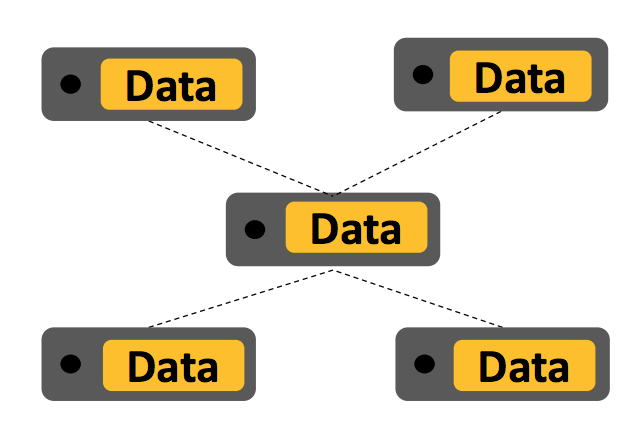
\includegraphics[width=0.8\textwidth]{rep1}

    Create a \textit{replica set} by copying data across multiple machines...

\end{frame}

\begin{frame}
    \frametitle{Replication}

    \centering
        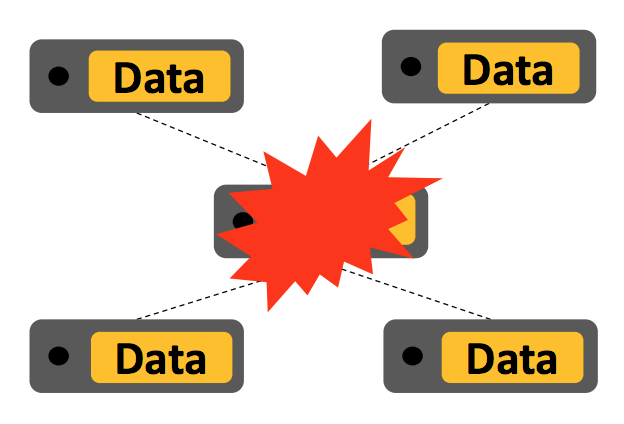
\includegraphics[width=0.8\textwidth]{rep2}

        ...So when one machine goes down...
\end{frame}

\begin{frame}
    \frametitle{Replication}

    \centering
        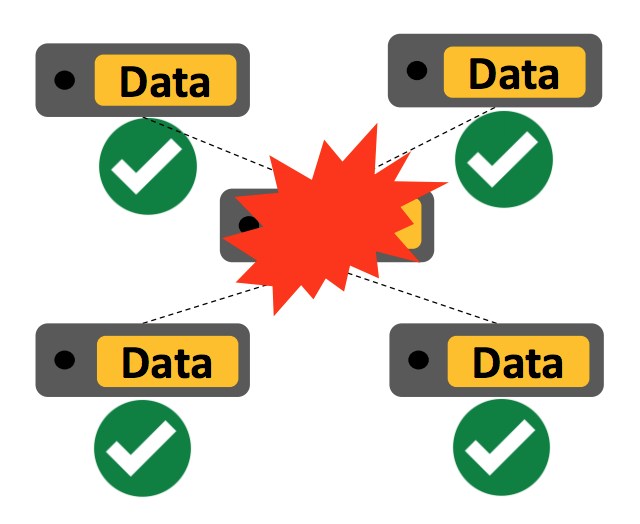
\includegraphics[width=0.8\textwidth]{rep3}

        ... The data (and hence the service) are still available!
\end{frame}

\begin{frame}
    \frametitle{Replication in MongoDB}

    \centering
    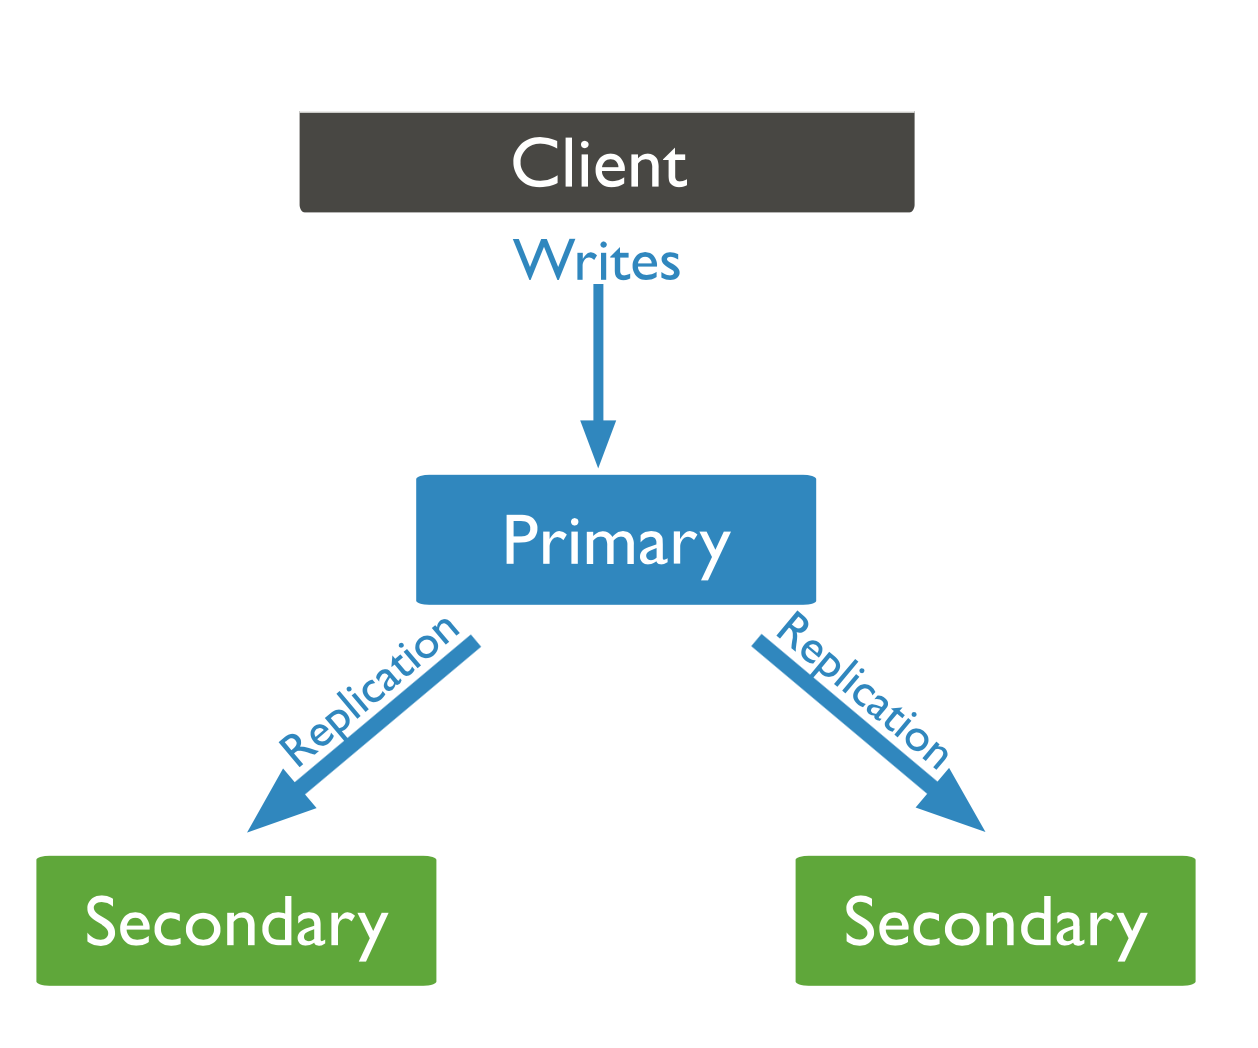
\includegraphics[height=.625\textheight]{../images/mongodbreplicaset.png}

    MongoDB uses a \textit{Primary-Backup} strategy. \textbf{One} Primary, \textbf{the rest} are Secondaries.

    All \textbf{write} operations must go through the Primary.
\end{frame}

\begin{frame}
    \frametitle{Replication in MongoDB}
    
    \centering
    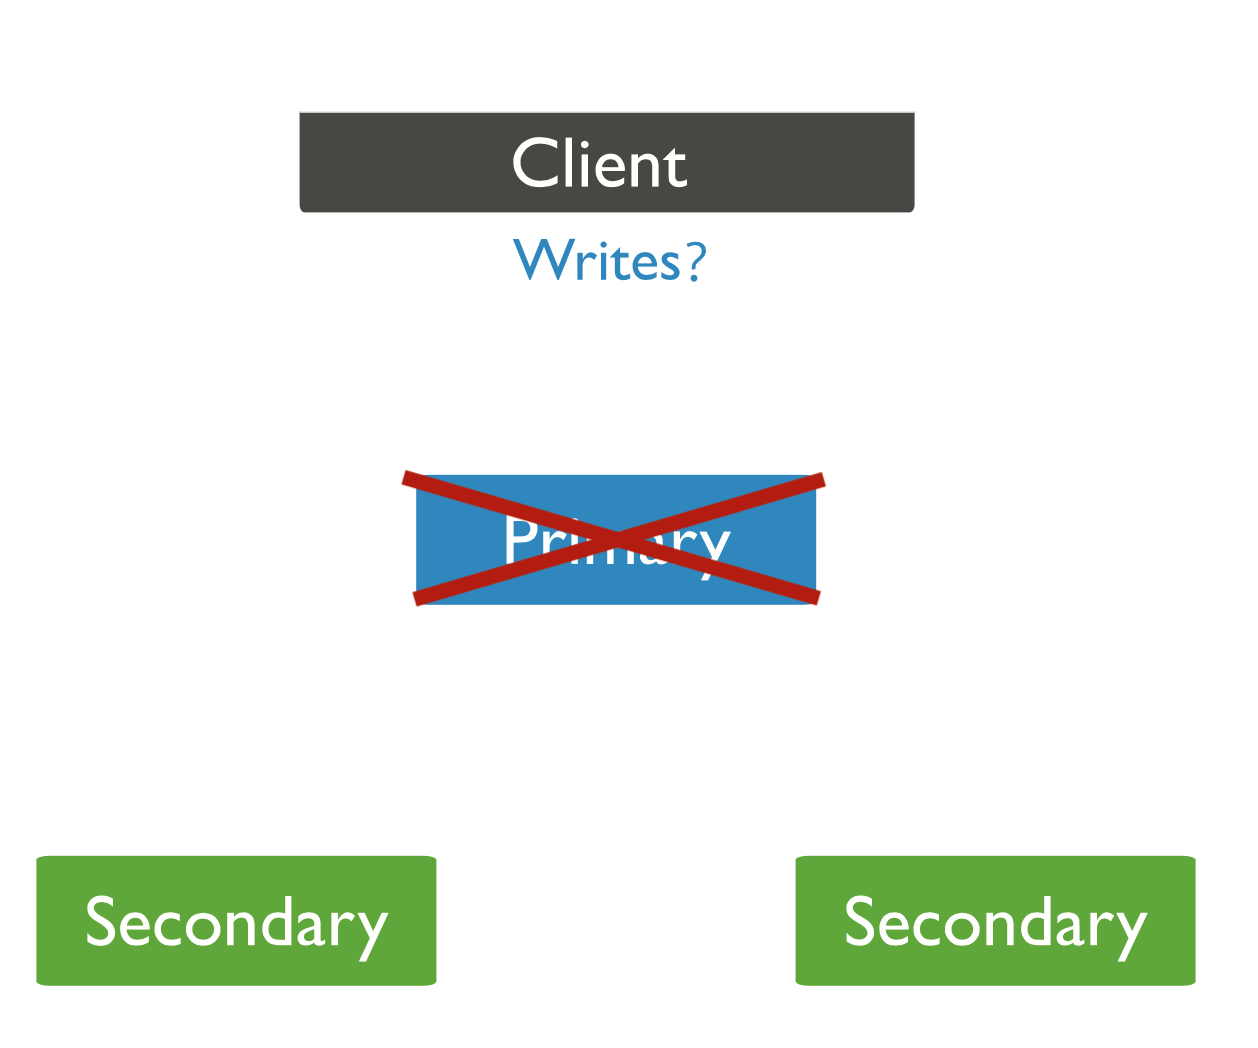
\includegraphics[height=.625\textheight]{../images/mongodbprimaryfail.png}

    If a primary is down, \textbf{no write operations} can be acknowledged.

\end{frame}

\begin{frame}
    \frametitle{Replication in MongoDB}
    
    \centering
    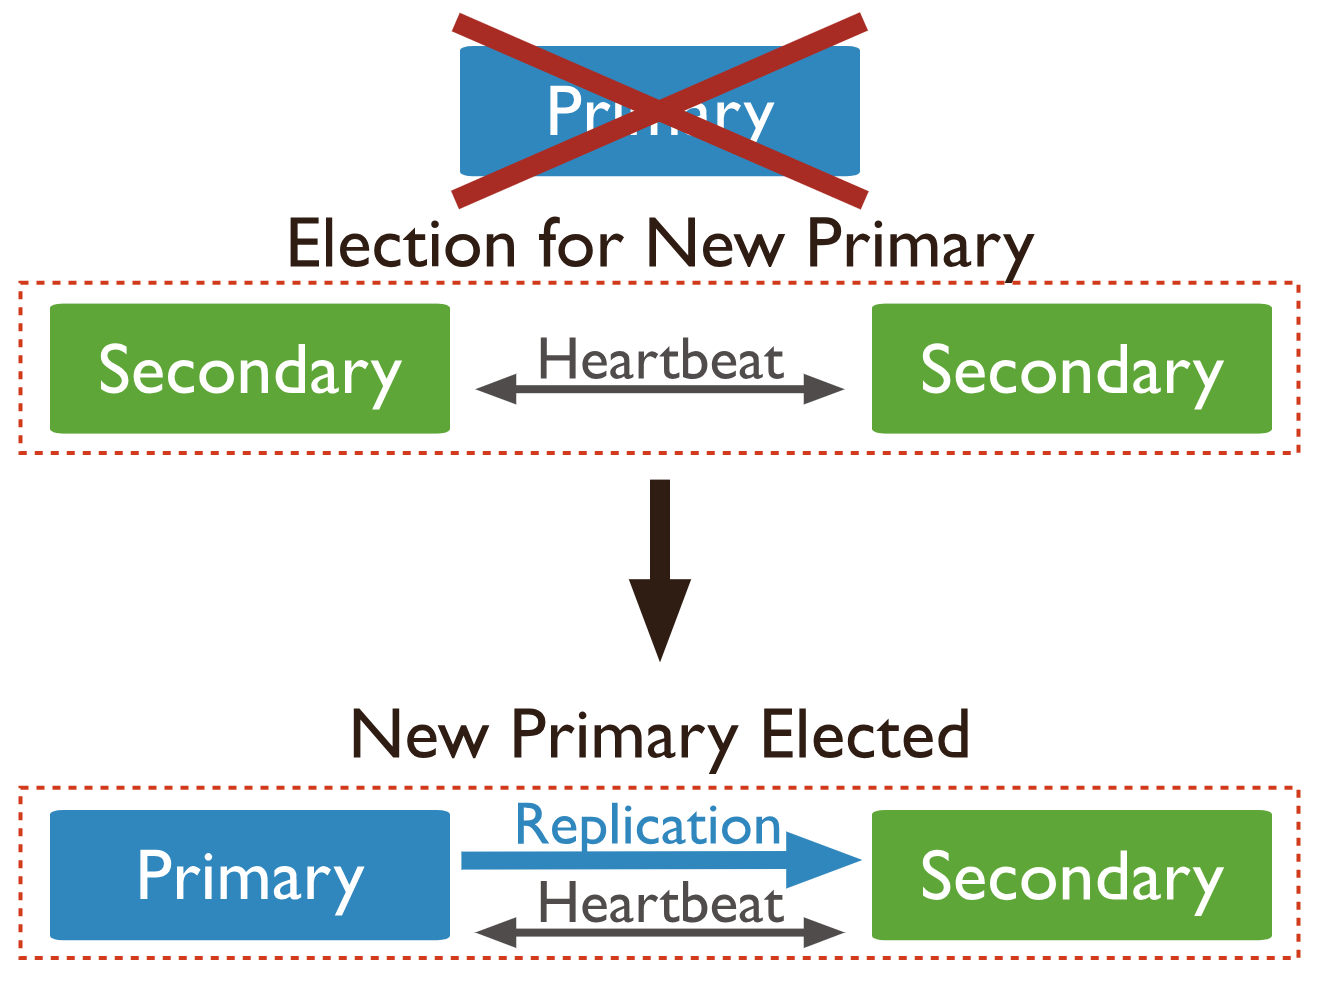
\includegraphics[height=.625\textheight]{../images/mongodbelection.png}

    When the Primary fails, all working Secondaries perform an \textit{election} to select a new primary.
\end{frame}

\begin{frame}
    \frametitle{MongoDB Journal}

    \begin{center}
    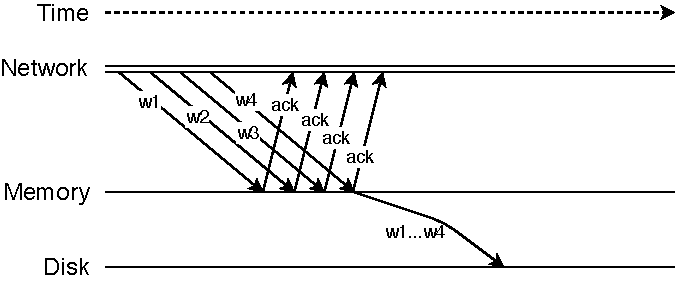
\includegraphics[height=0.5\textheight]{../images/Buffering1.pdf}
    A journal is used to \textit{recover} after failure by "replaying" the operations.

    MongoDB with \textbf{Journaled} writes will \textbf{send acknowledgements} without them going to disk!

    \end{center}

\end{frame}

\begin{frame}
    \frametitle{MongoDB Specifics}

    MongoDB allows users to configure the \textit{strength} of their writes through the \textbf{write concern}. 
    
    Stronger = harder to lose, but longer to acknowledge.

    \pause

    \begin{description}
        \item[\textbf{Primary}] Operation is applied to the data on the primary
        \item[\textbf{Journaled}] Operation is applied to data and added to Journal on the primary
        \item[\textbf{Majority}] Operation is applied and added to Journal on the \textit{majority} of the replicas.
    \end{description}

    \pause 

    Under \textbf{Majority} write concern, there should be \textit{no write loss!}

\end{frame}

\begin{frame}
    \frametitle{What has been done}
    \citet{cap} conjectured that databases cannot be simultaneously \textit{Consistent, Available and Network failure tolerant}. \citet{cap-proof} proved this result. \\
    $\Rightarrow$ There are limits to the capability of any database!

    A tool "Jepsen" was developed to test effects of \textit{Network failures} on databases. \citep{jepsen-2013, jepsen-2017, jepsen-2018}

    And \citet{correlated-crash} studied durability when \textit{all} replicas fail, with a focus on file systems. \\
    Note: probability of \textit{all} replicas failing is \textbf{incredibly slim}.

    \begin{center}
        There is \textbf{no work} on durability of distributed databases under single machine failures.
    \end{center}

\end{frame}

\begin{frame}
    \frametitle{The Aim}
    \begin{center}
        \textit{
            To equip users and designers of distributed databases with the means to protect their systems from durability failures.
        }
    \end{center}
\end{frame}

% \begin{frame}
%     \frametitle{How we achieve this}
%     \begin{itemize}
%         \item Enhancing their understanding of the \textbf{sources of data loss}.
%         \item Providing them with the means to \textbf{quantitatively measure durability} of their systems.
%         \item Empirically evaluating the \textbf{tradeoffs} between durable and performant configurations.
%         \item Offering a methodology to reason about and measure the \textbf{time it takes} for a write to become durable.
%     \end{itemize}
% \end{frame}

\begin{frame}

    \frametitle{Thesis Contributions}

    \begin{itemize}
        \item \textbf{Categorisation of \textit{scenarios} that result in write loss.}
        \item \textbf{Design of an experiment capable of inducing write loss.}
        \item Algorithm to quantify the number of lost writes.
        \item \textbf{Empirical results to show that the experiment and algorithm work by detecting bugs in MongoDB 3.6-rc0.}
        \item Theoretical model for evaluating when a write becomes durable.
        \item \textbf{Estimation of when a write becomes durable on the \textit{Primary}, using rudimentary client-accessible measurements.}
        \item \textbf{An empirical study of time-till-durability on the \textit{Primary} for acknowledged writes.}
    \end{itemize}

\end{frame}

% \begin{frame}
%     \frametitle{Contributions (extra)}

%     \begin{itemize}
%         \item An experiment design capable of inducing a loss of writes, producing an execution history of all events in the process.
%         \item The algorithm used to process the execution history and quantify the amount of durability failures presented by the execution
%         \item A novel theoretical model for evaluating the time it takes for an acknowledged write to become durable.
%     \end{itemize}
% \end{frame}

\section{Detecting and Quantifying Durability Failures}

\begin{frame}
    \frametitle{Big picture}

    \begin{center}
    Can we create a scenario that \textit{forces} MongoDB to lose a write?

    How big is the impact of these scenarios?
    \end{center}

\end{frame}

\begin{frame}
    \frametitle{Write Loss scenario}

    \centering
    \begin{figure}
        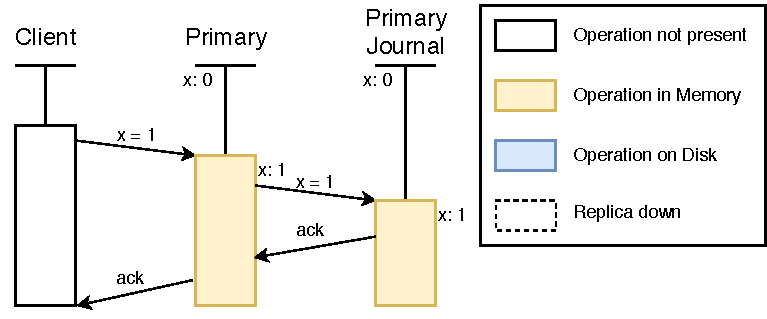
\includegraphics[width=0.9\textwidth]{../images/np1.pdf}
    \end{figure}
    We issue a \textbf{Journaled} write and get an \textit{acknowledgement}.

\end{frame}

\begin{frame}
    \frametitle{Write Loss scenario}

    \centering
    \begin{figure}
        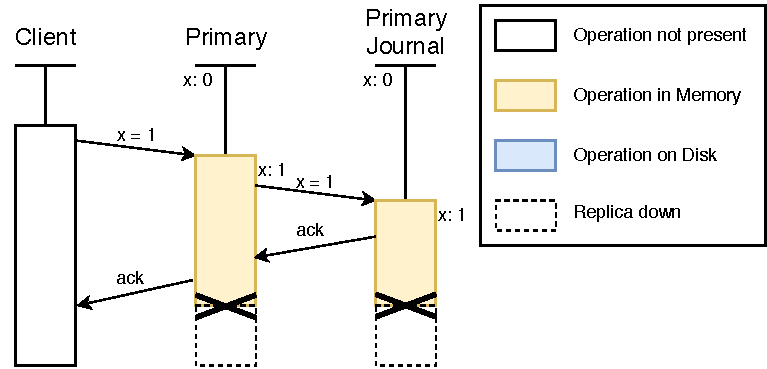
\includegraphics[width=0.9\textwidth]{../images/np2.pdf}
    \end{figure}
    The Primary \textit{crashes}.
\end{frame}

\begin{frame}
    \frametitle{Write Loss scenario}

    \centering
    \begin{figure}
        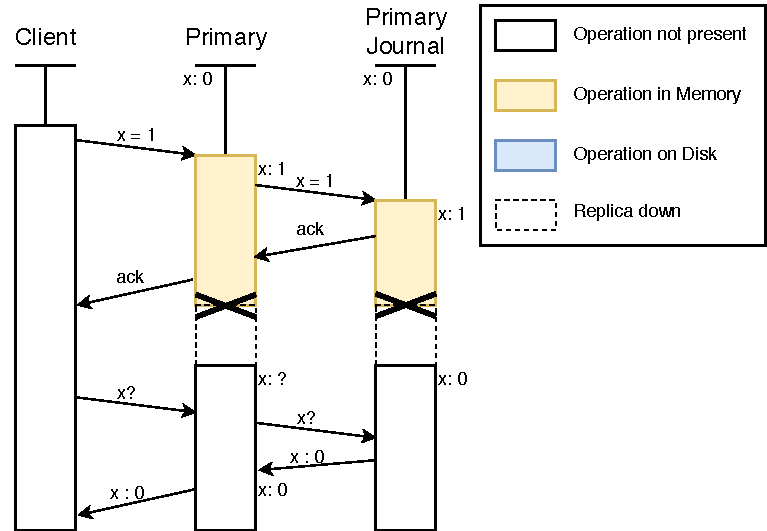
\includegraphics[width=0.9\textwidth]{../images/np3.pdf}
    \end{figure}
    The Primary \textit{loses} any writes still \textit{in-memory}.
\end{frame}

\begin{frame}
    \frametitle{How do we do this empirically?}
    We created a tool that:
    \begin{itemize}
        \item Configures a replica set
        \item Stresses it with reads and writes
        \item Crashes the Primary \textbf{100 seconds} into experiment.
        \item Recovers the (old) Primary \textbf{200 seconds} into experiment.
        \item Observes \textit{incorrect values} in queries.
    \end{itemize}
\end{frame}

% \begin{frame}
%     \frametitle{Experiment Design}

%     \begin{itemize}
%         \item 3 virtual machines configured as 1 MongoDB replica set
%         \item 3 stages
%         \item 2 failure types
%         \item Workload of single document operations
%         \item Output as a \textit{execution history}
%     \end{itemize}

% \end{frame}

% \begin{frame}
%     \frametitle{Experiment stages}

%     \begin{description}
%         \item[\textbf{Standard operation}] The virtual machines are started in "Headless" mode and run normally.
%         \item[\textbf{Operating under failure}] A failure was induced on the primary. Depending on the type of failure, the machine may disconnect from the replica set initiating an election. 
%         \item[\textbf{Recovery}] The failure is reverted and the failed machine is connected back to the replica set if it hasn't already.
%     \end{description}

%     Each of the threes stages occupies a third of the experiment time: 
% \end{frame}

% \begin{frame}
%     \frametitle{Failures}

%     \begin{description}
%         \item[\textbf{ACPI Shutdown}] Sends an ACPI shutdown signal to the primary VM to trigger a graceful shutdown of the machine.
%         \item[\textbf{Hard Poweroff}] Simulates an abrupt power failure, which turns the VM off immediately.
%     \end{description}

% \end{frame}

% \begin{frame}
%     \frametitle{Workload}

%     3 types of operations:
%     \begin{itemize}
%         \item Create Document
%         \item Read Document
%         \item Update Document
%     \end{itemize}

% \end{frame}

\begin{frame}
    \frametitle{Results - Write Loss: Mongo 4.0}
    \centering
    \begin{figure}
        \scalebox{.5}{%% Creator: Matplotlib, PGF backend
%%
%% To include the figure in your LaTeX document, write
%%   \input{<filename>.pgf}
%%
%% Make sure the required packages are loaded in your preamble
%%   \usepackage{pgf}
%%
%% Figures using additional raster images can only be included by \input if
%% they are in the same directory as the main LaTeX file. For loading figures
%% from other directories you can use the `import` package
%%   \usepackage{import}
%% and then include the figures with
%%   \import{<path to file>}{<filename>.pgf}
%%
%% Matplotlib used the following preamble
%%   \usepackage[utf8x]{inputenc}
%%   \usepackage[T1]{fontenc}
%%   \usepackage{lmodern}
%%
\begingroup%
\makeatletter%
\begin{pgfpicture}%
\pgfpathrectangle{\pgfpointorigin}{\pgfqpoint{6.400000in}{4.800000in}}%
\pgfusepath{use as bounding box, clip}%
\begin{pgfscope}%
\pgfsetbuttcap%
\pgfsetmiterjoin%
\definecolor{currentfill}{rgb}{1.000000,1.000000,1.000000}%
\pgfsetfillcolor{currentfill}%
\pgfsetlinewidth{0.000000pt}%
\definecolor{currentstroke}{rgb}{1.000000,1.000000,1.000000}%
\pgfsetstrokecolor{currentstroke}%
\pgfsetdash{}{0pt}%
\pgfpathmoveto{\pgfqpoint{0.000000in}{0.000000in}}%
\pgfpathlineto{\pgfqpoint{6.400000in}{0.000000in}}%
\pgfpathlineto{\pgfqpoint{6.400000in}{4.800000in}}%
\pgfpathlineto{\pgfqpoint{0.000000in}{4.800000in}}%
\pgfpathclose%
\pgfusepath{fill}%
\end{pgfscope}%
\begin{pgfscope}%
\pgfsetbuttcap%
\pgfsetmiterjoin%
\definecolor{currentfill}{rgb}{1.000000,1.000000,1.000000}%
\pgfsetfillcolor{currentfill}%
\pgfsetlinewidth{0.000000pt}%
\definecolor{currentstroke}{rgb}{0.000000,0.000000,0.000000}%
\pgfsetstrokecolor{currentstroke}%
\pgfsetstrokeopacity{0.000000}%
\pgfsetdash{}{0pt}%
\pgfpathmoveto{\pgfqpoint{0.800000in}{0.528000in}}%
\pgfpathlineto{\pgfqpoint{5.760000in}{0.528000in}}%
\pgfpathlineto{\pgfqpoint{5.760000in}{4.224000in}}%
\pgfpathlineto{\pgfqpoint{0.800000in}{4.224000in}}%
\pgfpathclose%
\pgfusepath{fill}%
\end{pgfscope}%
\begin{pgfscope}%
\pgfsetbuttcap%
\pgfsetroundjoin%
\definecolor{currentfill}{rgb}{0.000000,0.000000,0.000000}%
\pgfsetfillcolor{currentfill}%
\pgfsetlinewidth{0.803000pt}%
\definecolor{currentstroke}{rgb}{0.000000,0.000000,0.000000}%
\pgfsetstrokecolor{currentstroke}%
\pgfsetdash{}{0pt}%
\pgfsys@defobject{currentmarker}{\pgfqpoint{0.000000in}{-0.048611in}}{\pgfqpoint{0.000000in}{0.000000in}}{%
\pgfpathmoveto{\pgfqpoint{0.000000in}{0.000000in}}%
\pgfpathlineto{\pgfqpoint{0.000000in}{-0.048611in}}%
\pgfusepath{stroke,fill}%
}%
\begin{pgfscope}%
\pgfsys@transformshift{1.025455in}{0.528000in}%
\pgfsys@useobject{currentmarker}{}%
\end{pgfscope}%
\end{pgfscope}%
\begin{pgfscope}%
\pgftext[x=1.025455in,y=0.430778in,,top]{\fontsize{11.000000}{13.200000}\selectfont \(\displaystyle 0\)}%
\end{pgfscope}%
\begin{pgfscope}%
\pgfsetbuttcap%
\pgfsetroundjoin%
\definecolor{currentfill}{rgb}{0.000000,0.000000,0.000000}%
\pgfsetfillcolor{currentfill}%
\pgfsetlinewidth{0.803000pt}%
\definecolor{currentstroke}{rgb}{0.000000,0.000000,0.000000}%
\pgfsetstrokecolor{currentstroke}%
\pgfsetdash{}{0pt}%
\pgfsys@defobject{currentmarker}{\pgfqpoint{0.000000in}{-0.048611in}}{\pgfqpoint{0.000000in}{0.000000in}}{%
\pgfpathmoveto{\pgfqpoint{0.000000in}{0.000000in}}%
\pgfpathlineto{\pgfqpoint{0.000000in}{-0.048611in}}%
\pgfusepath{stroke,fill}%
}%
\begin{pgfscope}%
\pgfsys@transformshift{1.762234in}{0.528000in}%
\pgfsys@useobject{currentmarker}{}%
\end{pgfscope}%
\end{pgfscope}%
\begin{pgfscope}%
\pgftext[x=1.762234in,y=0.430778in,,top]{\fontsize{11.000000}{13.200000}\selectfont \(\displaystyle 50\)}%
\end{pgfscope}%
\begin{pgfscope}%
\pgfsetbuttcap%
\pgfsetroundjoin%
\definecolor{currentfill}{rgb}{0.000000,0.000000,0.000000}%
\pgfsetfillcolor{currentfill}%
\pgfsetlinewidth{0.803000pt}%
\definecolor{currentstroke}{rgb}{0.000000,0.000000,0.000000}%
\pgfsetstrokecolor{currentstroke}%
\pgfsetdash{}{0pt}%
\pgfsys@defobject{currentmarker}{\pgfqpoint{0.000000in}{-0.048611in}}{\pgfqpoint{0.000000in}{0.000000in}}{%
\pgfpathmoveto{\pgfqpoint{0.000000in}{0.000000in}}%
\pgfpathlineto{\pgfqpoint{0.000000in}{-0.048611in}}%
\pgfusepath{stroke,fill}%
}%
\begin{pgfscope}%
\pgfsys@transformshift{2.499014in}{0.528000in}%
\pgfsys@useobject{currentmarker}{}%
\end{pgfscope}%
\end{pgfscope}%
\begin{pgfscope}%
\pgftext[x=2.499014in,y=0.430778in,,top]{\fontsize{11.000000}{13.200000}\selectfont \(\displaystyle 100\)}%
\end{pgfscope}%
\begin{pgfscope}%
\pgfsetbuttcap%
\pgfsetroundjoin%
\definecolor{currentfill}{rgb}{0.000000,0.000000,0.000000}%
\pgfsetfillcolor{currentfill}%
\pgfsetlinewidth{0.803000pt}%
\definecolor{currentstroke}{rgb}{0.000000,0.000000,0.000000}%
\pgfsetstrokecolor{currentstroke}%
\pgfsetdash{}{0pt}%
\pgfsys@defobject{currentmarker}{\pgfqpoint{0.000000in}{-0.048611in}}{\pgfqpoint{0.000000in}{0.000000in}}{%
\pgfpathmoveto{\pgfqpoint{0.000000in}{0.000000in}}%
\pgfpathlineto{\pgfqpoint{0.000000in}{-0.048611in}}%
\pgfusepath{stroke,fill}%
}%
\begin{pgfscope}%
\pgfsys@transformshift{3.235793in}{0.528000in}%
\pgfsys@useobject{currentmarker}{}%
\end{pgfscope}%
\end{pgfscope}%
\begin{pgfscope}%
\pgftext[x=3.235793in,y=0.430778in,,top]{\fontsize{11.000000}{13.200000}\selectfont \(\displaystyle 150\)}%
\end{pgfscope}%
\begin{pgfscope}%
\pgfsetbuttcap%
\pgfsetroundjoin%
\definecolor{currentfill}{rgb}{0.000000,0.000000,0.000000}%
\pgfsetfillcolor{currentfill}%
\pgfsetlinewidth{0.803000pt}%
\definecolor{currentstroke}{rgb}{0.000000,0.000000,0.000000}%
\pgfsetstrokecolor{currentstroke}%
\pgfsetdash{}{0pt}%
\pgfsys@defobject{currentmarker}{\pgfqpoint{0.000000in}{-0.048611in}}{\pgfqpoint{0.000000in}{0.000000in}}{%
\pgfpathmoveto{\pgfqpoint{0.000000in}{0.000000in}}%
\pgfpathlineto{\pgfqpoint{0.000000in}{-0.048611in}}%
\pgfusepath{stroke,fill}%
}%
\begin{pgfscope}%
\pgfsys@transformshift{3.972573in}{0.528000in}%
\pgfsys@useobject{currentmarker}{}%
\end{pgfscope}%
\end{pgfscope}%
\begin{pgfscope}%
\pgftext[x=3.972573in,y=0.430778in,,top]{\fontsize{11.000000}{13.200000}\selectfont \(\displaystyle 200\)}%
\end{pgfscope}%
\begin{pgfscope}%
\pgfsetbuttcap%
\pgfsetroundjoin%
\definecolor{currentfill}{rgb}{0.000000,0.000000,0.000000}%
\pgfsetfillcolor{currentfill}%
\pgfsetlinewidth{0.803000pt}%
\definecolor{currentstroke}{rgb}{0.000000,0.000000,0.000000}%
\pgfsetstrokecolor{currentstroke}%
\pgfsetdash{}{0pt}%
\pgfsys@defobject{currentmarker}{\pgfqpoint{0.000000in}{-0.048611in}}{\pgfqpoint{0.000000in}{0.000000in}}{%
\pgfpathmoveto{\pgfqpoint{0.000000in}{0.000000in}}%
\pgfpathlineto{\pgfqpoint{0.000000in}{-0.048611in}}%
\pgfusepath{stroke,fill}%
}%
\begin{pgfscope}%
\pgfsys@transformshift{4.709352in}{0.528000in}%
\pgfsys@useobject{currentmarker}{}%
\end{pgfscope}%
\end{pgfscope}%
\begin{pgfscope}%
\pgftext[x=4.709352in,y=0.430778in,,top]{\fontsize{11.000000}{13.200000}\selectfont \(\displaystyle 250\)}%
\end{pgfscope}%
\begin{pgfscope}%
\pgfsetbuttcap%
\pgfsetroundjoin%
\definecolor{currentfill}{rgb}{0.000000,0.000000,0.000000}%
\pgfsetfillcolor{currentfill}%
\pgfsetlinewidth{0.803000pt}%
\definecolor{currentstroke}{rgb}{0.000000,0.000000,0.000000}%
\pgfsetstrokecolor{currentstroke}%
\pgfsetdash{}{0pt}%
\pgfsys@defobject{currentmarker}{\pgfqpoint{0.000000in}{-0.048611in}}{\pgfqpoint{0.000000in}{0.000000in}}{%
\pgfpathmoveto{\pgfqpoint{0.000000in}{0.000000in}}%
\pgfpathlineto{\pgfqpoint{0.000000in}{-0.048611in}}%
\pgfusepath{stroke,fill}%
}%
\begin{pgfscope}%
\pgfsys@transformshift{5.446132in}{0.528000in}%
\pgfsys@useobject{currentmarker}{}%
\end{pgfscope}%
\end{pgfscope}%
\begin{pgfscope}%
\pgftext[x=5.446132in,y=0.430778in,,top]{\fontsize{11.000000}{13.200000}\selectfont \(\displaystyle 300\)}%
\end{pgfscope}%
\begin{pgfscope}%
\pgftext[x=3.280000in,y=0.240271in,,top]{\fontsize{11.000000}{13.200000}\selectfont Time of experiment (in seconds)}%
\end{pgfscope}%
\begin{pgfscope}%
\pgfsetbuttcap%
\pgfsetroundjoin%
\definecolor{currentfill}{rgb}{0.000000,0.000000,0.000000}%
\pgfsetfillcolor{currentfill}%
\pgfsetlinewidth{0.803000pt}%
\definecolor{currentstroke}{rgb}{0.000000,0.000000,0.000000}%
\pgfsetstrokecolor{currentstroke}%
\pgfsetdash{}{0pt}%
\pgfsys@defobject{currentmarker}{\pgfqpoint{-0.048611in}{0.000000in}}{\pgfqpoint{0.000000in}{0.000000in}}{%
\pgfpathmoveto{\pgfqpoint{0.000000in}{0.000000in}}%
\pgfpathlineto{\pgfqpoint{-0.048611in}{0.000000in}}%
\pgfusepath{stroke,fill}%
}%
\begin{pgfscope}%
\pgfsys@transformshift{0.800000in}{0.696000in}%
\pgfsys@useobject{currentmarker}{}%
\end{pgfscope}%
\end{pgfscope}%
\begin{pgfscope}%
\pgftext[x=0.627981in,y=0.643378in,left,base]{\fontsize{11.000000}{13.200000}\selectfont \(\displaystyle 0\)}%
\end{pgfscope}%
\begin{pgfscope}%
\pgfsetbuttcap%
\pgfsetroundjoin%
\definecolor{currentfill}{rgb}{0.000000,0.000000,0.000000}%
\pgfsetfillcolor{currentfill}%
\pgfsetlinewidth{0.803000pt}%
\definecolor{currentstroke}{rgb}{0.000000,0.000000,0.000000}%
\pgfsetstrokecolor{currentstroke}%
\pgfsetdash{}{0pt}%
\pgfsys@defobject{currentmarker}{\pgfqpoint{-0.048611in}{0.000000in}}{\pgfqpoint{0.000000in}{0.000000in}}{%
\pgfpathmoveto{\pgfqpoint{0.000000in}{0.000000in}}%
\pgfpathlineto{\pgfqpoint{-0.048611in}{0.000000in}}%
\pgfusepath{stroke,fill}%
}%
\begin{pgfscope}%
\pgfsys@transformshift{0.800000in}{1.212923in}%
\pgfsys@useobject{currentmarker}{}%
\end{pgfscope}%
\end{pgfscope}%
\begin{pgfscope}%
\pgftext[x=0.553183in,y=1.160301in,left,base]{\fontsize{11.000000}{13.200000}\selectfont \(\displaystyle 20\)}%
\end{pgfscope}%
\begin{pgfscope}%
\pgfsetbuttcap%
\pgfsetroundjoin%
\definecolor{currentfill}{rgb}{0.000000,0.000000,0.000000}%
\pgfsetfillcolor{currentfill}%
\pgfsetlinewidth{0.803000pt}%
\definecolor{currentstroke}{rgb}{0.000000,0.000000,0.000000}%
\pgfsetstrokecolor{currentstroke}%
\pgfsetdash{}{0pt}%
\pgfsys@defobject{currentmarker}{\pgfqpoint{-0.048611in}{0.000000in}}{\pgfqpoint{0.000000in}{0.000000in}}{%
\pgfpathmoveto{\pgfqpoint{0.000000in}{0.000000in}}%
\pgfpathlineto{\pgfqpoint{-0.048611in}{0.000000in}}%
\pgfusepath{stroke,fill}%
}%
\begin{pgfscope}%
\pgfsys@transformshift{0.800000in}{1.729846in}%
\pgfsys@useobject{currentmarker}{}%
\end{pgfscope}%
\end{pgfscope}%
\begin{pgfscope}%
\pgftext[x=0.553183in,y=1.677224in,left,base]{\fontsize{11.000000}{13.200000}\selectfont \(\displaystyle 40\)}%
\end{pgfscope}%
\begin{pgfscope}%
\pgfsetbuttcap%
\pgfsetroundjoin%
\definecolor{currentfill}{rgb}{0.000000,0.000000,0.000000}%
\pgfsetfillcolor{currentfill}%
\pgfsetlinewidth{0.803000pt}%
\definecolor{currentstroke}{rgb}{0.000000,0.000000,0.000000}%
\pgfsetstrokecolor{currentstroke}%
\pgfsetdash{}{0pt}%
\pgfsys@defobject{currentmarker}{\pgfqpoint{-0.048611in}{0.000000in}}{\pgfqpoint{0.000000in}{0.000000in}}{%
\pgfpathmoveto{\pgfqpoint{0.000000in}{0.000000in}}%
\pgfpathlineto{\pgfqpoint{-0.048611in}{0.000000in}}%
\pgfusepath{stroke,fill}%
}%
\begin{pgfscope}%
\pgfsys@transformshift{0.800000in}{2.246769in}%
\pgfsys@useobject{currentmarker}{}%
\end{pgfscope}%
\end{pgfscope}%
\begin{pgfscope}%
\pgftext[x=0.553183in,y=2.194147in,left,base]{\fontsize{11.000000}{13.200000}\selectfont \(\displaystyle 60\)}%
\end{pgfscope}%
\begin{pgfscope}%
\pgfsetbuttcap%
\pgfsetroundjoin%
\definecolor{currentfill}{rgb}{0.000000,0.000000,0.000000}%
\pgfsetfillcolor{currentfill}%
\pgfsetlinewidth{0.803000pt}%
\definecolor{currentstroke}{rgb}{0.000000,0.000000,0.000000}%
\pgfsetstrokecolor{currentstroke}%
\pgfsetdash{}{0pt}%
\pgfsys@defobject{currentmarker}{\pgfqpoint{-0.048611in}{0.000000in}}{\pgfqpoint{0.000000in}{0.000000in}}{%
\pgfpathmoveto{\pgfqpoint{0.000000in}{0.000000in}}%
\pgfpathlineto{\pgfqpoint{-0.048611in}{0.000000in}}%
\pgfusepath{stroke,fill}%
}%
\begin{pgfscope}%
\pgfsys@transformshift{0.800000in}{2.763692in}%
\pgfsys@useobject{currentmarker}{}%
\end{pgfscope}%
\end{pgfscope}%
\begin{pgfscope}%
\pgftext[x=0.553183in,y=2.711070in,left,base]{\fontsize{11.000000}{13.200000}\selectfont \(\displaystyle 80\)}%
\end{pgfscope}%
\begin{pgfscope}%
\pgfsetbuttcap%
\pgfsetroundjoin%
\definecolor{currentfill}{rgb}{0.000000,0.000000,0.000000}%
\pgfsetfillcolor{currentfill}%
\pgfsetlinewidth{0.803000pt}%
\definecolor{currentstroke}{rgb}{0.000000,0.000000,0.000000}%
\pgfsetstrokecolor{currentstroke}%
\pgfsetdash{}{0pt}%
\pgfsys@defobject{currentmarker}{\pgfqpoint{-0.048611in}{0.000000in}}{\pgfqpoint{0.000000in}{0.000000in}}{%
\pgfpathmoveto{\pgfqpoint{0.000000in}{0.000000in}}%
\pgfpathlineto{\pgfqpoint{-0.048611in}{0.000000in}}%
\pgfusepath{stroke,fill}%
}%
\begin{pgfscope}%
\pgfsys@transformshift{0.800000in}{3.280615in}%
\pgfsys@useobject{currentmarker}{}%
\end{pgfscope}%
\end{pgfscope}%
\begin{pgfscope}%
\pgftext[x=0.478386in,y=3.227993in,left,base]{\fontsize{11.000000}{13.200000}\selectfont \(\displaystyle 100\)}%
\end{pgfscope}%
\begin{pgfscope}%
\pgfsetbuttcap%
\pgfsetroundjoin%
\definecolor{currentfill}{rgb}{0.000000,0.000000,0.000000}%
\pgfsetfillcolor{currentfill}%
\pgfsetlinewidth{0.803000pt}%
\definecolor{currentstroke}{rgb}{0.000000,0.000000,0.000000}%
\pgfsetstrokecolor{currentstroke}%
\pgfsetdash{}{0pt}%
\pgfsys@defobject{currentmarker}{\pgfqpoint{-0.048611in}{0.000000in}}{\pgfqpoint{0.000000in}{0.000000in}}{%
\pgfpathmoveto{\pgfqpoint{0.000000in}{0.000000in}}%
\pgfpathlineto{\pgfqpoint{-0.048611in}{0.000000in}}%
\pgfusepath{stroke,fill}%
}%
\begin{pgfscope}%
\pgfsys@transformshift{0.800000in}{3.797538in}%
\pgfsys@useobject{currentmarker}{}%
\end{pgfscope}%
\end{pgfscope}%
\begin{pgfscope}%
\pgftext[x=0.478386in,y=3.744916in,left,base]{\fontsize{11.000000}{13.200000}\selectfont \(\displaystyle 120\)}%
\end{pgfscope}%
\begin{pgfscope}%
\pgftext[x=0.422830in,y=2.376000in,,bottom,rotate=90.000000]{\fontsize{11.000000}{13.200000}\selectfont Number of writes lost}%
\end{pgfscope}%
\begin{pgfscope}%
\pgfpathrectangle{\pgfqpoint{0.800000in}{0.528000in}}{\pgfqpoint{4.960000in}{3.696000in}}%
\pgfusepath{clip}%
\pgfsetrectcap%
\pgfsetroundjoin%
\pgfsetlinewidth{1.505625pt}%
\definecolor{currentstroke}{rgb}{0.121569,0.466667,0.705882}%
\pgfsetstrokecolor{currentstroke}%
\pgfsetdash{}{0pt}%
\pgfpathmoveto{\pgfqpoint{1.025455in}{0.696000in}}%
\pgfpathlineto{\pgfqpoint{2.469542in}{0.696000in}}%
\pgfpathlineto{\pgfqpoint{2.484278in}{2.246769in}}%
\pgfpathlineto{\pgfqpoint{2.499014in}{4.056000in}}%
\pgfpathlineto{\pgfqpoint{2.513749in}{1.884923in}}%
\pgfpathlineto{\pgfqpoint{2.528485in}{0.696000in}}%
\pgfpathlineto{\pgfqpoint{5.534545in}{0.696000in}}%
\pgfpathlineto{\pgfqpoint{5.534545in}{0.696000in}}%
\pgfusepath{stroke}%
\end{pgfscope}%
\begin{pgfscope}%
\pgfpathrectangle{\pgfqpoint{0.800000in}{0.528000in}}{\pgfqpoint{4.960000in}{3.696000in}}%
\pgfusepath{clip}%
\pgfsetrectcap%
\pgfsetroundjoin%
\pgfsetlinewidth{1.505625pt}%
\definecolor{currentstroke}{rgb}{1.000000,0.498039,0.054902}%
\pgfsetstrokecolor{currentstroke}%
\pgfsetdash{}{0pt}%
\pgfpathmoveto{\pgfqpoint{1.025455in}{0.696000in}}%
\pgfpathlineto{\pgfqpoint{5.534545in}{0.696000in}}%
\pgfpathlineto{\pgfqpoint{5.534545in}{0.696000in}}%
\pgfusepath{stroke}%
\end{pgfscope}%
\begin{pgfscope}%
\pgfsetrectcap%
\pgfsetmiterjoin%
\pgfsetlinewidth{0.803000pt}%
\definecolor{currentstroke}{rgb}{0.000000,0.000000,0.000000}%
\pgfsetstrokecolor{currentstroke}%
\pgfsetdash{}{0pt}%
\pgfpathmoveto{\pgfqpoint{0.800000in}{0.528000in}}%
\pgfpathlineto{\pgfqpoint{0.800000in}{4.224000in}}%
\pgfusepath{stroke}%
\end{pgfscope}%
\begin{pgfscope}%
\pgfsetrectcap%
\pgfsetmiterjoin%
\pgfsetlinewidth{0.803000pt}%
\definecolor{currentstroke}{rgb}{0.000000,0.000000,0.000000}%
\pgfsetstrokecolor{currentstroke}%
\pgfsetdash{}{0pt}%
\pgfpathmoveto{\pgfqpoint{5.760000in}{0.528000in}}%
\pgfpathlineto{\pgfqpoint{5.760000in}{4.224000in}}%
\pgfusepath{stroke}%
\end{pgfscope}%
\begin{pgfscope}%
\pgfsetrectcap%
\pgfsetmiterjoin%
\pgfsetlinewidth{0.803000pt}%
\definecolor{currentstroke}{rgb}{0.000000,0.000000,0.000000}%
\pgfsetstrokecolor{currentstroke}%
\pgfsetdash{}{0pt}%
\pgfpathmoveto{\pgfqpoint{0.800000in}{0.528000in}}%
\pgfpathlineto{\pgfqpoint{5.760000in}{0.528000in}}%
\pgfusepath{stroke}%
\end{pgfscope}%
\begin{pgfscope}%
\pgfsetrectcap%
\pgfsetmiterjoin%
\pgfsetlinewidth{0.803000pt}%
\definecolor{currentstroke}{rgb}{0.000000,0.000000,0.000000}%
\pgfsetstrokecolor{currentstroke}%
\pgfsetdash{}{0pt}%
\pgfpathmoveto{\pgfqpoint{0.800000in}{4.224000in}}%
\pgfpathlineto{\pgfqpoint{5.760000in}{4.224000in}}%
\pgfusepath{stroke}%
\end{pgfscope}%
\begin{pgfscope}%
\pgfsetbuttcap%
\pgfsetmiterjoin%
\definecolor{currentfill}{rgb}{1.000000,1.000000,1.000000}%
\pgfsetfillcolor{currentfill}%
\pgfsetfillopacity{0.800000}%
\pgfsetlinewidth{1.003750pt}%
\definecolor{currentstroke}{rgb}{0.800000,0.800000,0.800000}%
\pgfsetstrokecolor{currentstroke}%
\pgfsetstrokeopacity{0.800000}%
\pgfsetdash{}{0pt}%
\pgfpathmoveto{\pgfqpoint{3.591379in}{3.675698in}}%
\pgfpathlineto{\pgfqpoint{5.653056in}{3.675698in}}%
\pgfpathquadraticcurveto{\pgfqpoint{5.683611in}{3.675698in}}{\pgfqpoint{5.683611in}{3.706254in}}%
\pgfpathlineto{\pgfqpoint{5.683611in}{4.117056in}}%
\pgfpathquadraticcurveto{\pgfqpoint{5.683611in}{4.147611in}}{\pgfqpoint{5.653056in}{4.147611in}}%
\pgfpathlineto{\pgfqpoint{3.591379in}{4.147611in}}%
\pgfpathquadraticcurveto{\pgfqpoint{3.560823in}{4.147611in}}{\pgfqpoint{3.560823in}{4.117056in}}%
\pgfpathlineto{\pgfqpoint{3.560823in}{3.706254in}}%
\pgfpathquadraticcurveto{\pgfqpoint{3.560823in}{3.675698in}}{\pgfqpoint{3.591379in}{3.675698in}}%
\pgfpathclose%
\pgfusepath{stroke,fill}%
\end{pgfscope}%
\begin{pgfscope}%
\pgfsetrectcap%
\pgfsetroundjoin%
\pgfsetlinewidth{1.505625pt}%
\definecolor{currentstroke}{rgb}{0.121569,0.466667,0.705882}%
\pgfsetstrokecolor{currentstroke}%
\pgfsetdash{}{0pt}%
\pgfpathmoveto{\pgfqpoint{3.621934in}{4.033028in}}%
\pgfpathlineto{\pgfqpoint{3.927490in}{4.033028in}}%
\pgfusepath{stroke}%
\end{pgfscope}%
\begin{pgfscope}%
\pgftext[x=4.049712in,y=3.979556in,left,base]{\fontsize{11.000000}{13.200000}\selectfont Journaled write concern}%
\end{pgfscope}%
\begin{pgfscope}%
\pgfsetrectcap%
\pgfsetroundjoin%
\pgfsetlinewidth{1.505625pt}%
\definecolor{currentstroke}{rgb}{1.000000,0.498039,0.054902}%
\pgfsetstrokecolor{currentstroke}%
\pgfsetdash{}{0pt}%
\pgfpathmoveto{\pgfqpoint{3.621934in}{3.819988in}}%
\pgfpathlineto{\pgfqpoint{3.927490in}{3.819988in}}%
\pgfusepath{stroke}%
\end{pgfscope}%
\begin{pgfscope}%
\pgftext[x=4.049712in,y=3.766516in,left,base]{\fontsize{11.000000}{13.200000}\selectfont Majority write concern}%
\end{pgfscope}%
\end{pgfpicture}%
\makeatother%
\endgroup%
}
        \caption{Distribution of write loss for every second in MongoDB 4.0.}
    \end{figure}

\end{frame}

\begin{frame}
    \frametitle{Results - Write Loss: Mongo 3.6-rc0}
    
    \begin{figure}
        \scalebox{.5}{%% Creator: Matplotlib, PGF backend
%%
%% To include the figure in your LaTeX document, write
%%   \input{<filename>.pgf}
%%
%% Make sure the required packages are loaded in your preamble
%%   \usepackage{pgf}
%%
%% Figures using additional raster images can only be included by \input if
%% they are in the same directory as the main LaTeX file. For loading figures
%% from other directories you can use the `import` package
%%   \usepackage{import}
%% and then include the figures with
%%   \import{<path to file>}{<filename>.pgf}
%%
%% Matplotlib used the following preamble
%%   \usepackage[utf8x]{inputenc}
%%   \usepackage[T1]{fontenc}
%%   \usepackage{lmodern}
%%
\begingroup%
\makeatletter%
\begin{pgfpicture}%
\pgfpathrectangle{\pgfpointorigin}{\pgfqpoint{6.400000in}{4.800000in}}%
\pgfusepath{use as bounding box, clip}%
\begin{pgfscope}%
\pgfsetbuttcap%
\pgfsetmiterjoin%
\definecolor{currentfill}{rgb}{1.000000,1.000000,1.000000}%
\pgfsetfillcolor{currentfill}%
\pgfsetlinewidth{0.000000pt}%
\definecolor{currentstroke}{rgb}{1.000000,1.000000,1.000000}%
\pgfsetstrokecolor{currentstroke}%
\pgfsetdash{}{0pt}%
\pgfpathmoveto{\pgfqpoint{0.000000in}{0.000000in}}%
\pgfpathlineto{\pgfqpoint{6.400000in}{0.000000in}}%
\pgfpathlineto{\pgfqpoint{6.400000in}{4.800000in}}%
\pgfpathlineto{\pgfqpoint{0.000000in}{4.800000in}}%
\pgfpathclose%
\pgfusepath{fill}%
\end{pgfscope}%
\begin{pgfscope}%
\pgfsetbuttcap%
\pgfsetmiterjoin%
\definecolor{currentfill}{rgb}{1.000000,1.000000,1.000000}%
\pgfsetfillcolor{currentfill}%
\pgfsetlinewidth{0.000000pt}%
\definecolor{currentstroke}{rgb}{0.000000,0.000000,0.000000}%
\pgfsetstrokecolor{currentstroke}%
\pgfsetstrokeopacity{0.000000}%
\pgfsetdash{}{0pt}%
\pgfpathmoveto{\pgfqpoint{0.800000in}{0.528000in}}%
\pgfpathlineto{\pgfqpoint{5.760000in}{0.528000in}}%
\pgfpathlineto{\pgfqpoint{5.760000in}{4.224000in}}%
\pgfpathlineto{\pgfqpoint{0.800000in}{4.224000in}}%
\pgfpathclose%
\pgfusepath{fill}%
\end{pgfscope}%
\begin{pgfscope}%
\pgfsetbuttcap%
\pgfsetroundjoin%
\definecolor{currentfill}{rgb}{0.000000,0.000000,0.000000}%
\pgfsetfillcolor{currentfill}%
\pgfsetlinewidth{0.803000pt}%
\definecolor{currentstroke}{rgb}{0.000000,0.000000,0.000000}%
\pgfsetstrokecolor{currentstroke}%
\pgfsetdash{}{0pt}%
\pgfsys@defobject{currentmarker}{\pgfqpoint{0.000000in}{-0.048611in}}{\pgfqpoint{0.000000in}{0.000000in}}{%
\pgfpathmoveto{\pgfqpoint{0.000000in}{0.000000in}}%
\pgfpathlineto{\pgfqpoint{0.000000in}{-0.048611in}}%
\pgfusepath{stroke,fill}%
}%
\begin{pgfscope}%
\pgfsys@transformshift{1.025455in}{0.528000in}%
\pgfsys@useobject{currentmarker}{}%
\end{pgfscope}%
\end{pgfscope}%
\begin{pgfscope}%
\pgftext[x=1.025455in,y=0.430778in,,top]{\fontsize{11.000000}{13.200000}\selectfont \(\displaystyle 0\)}%
\end{pgfscope}%
\begin{pgfscope}%
\pgfsetbuttcap%
\pgfsetroundjoin%
\definecolor{currentfill}{rgb}{0.000000,0.000000,0.000000}%
\pgfsetfillcolor{currentfill}%
\pgfsetlinewidth{0.803000pt}%
\definecolor{currentstroke}{rgb}{0.000000,0.000000,0.000000}%
\pgfsetstrokecolor{currentstroke}%
\pgfsetdash{}{0pt}%
\pgfsys@defobject{currentmarker}{\pgfqpoint{0.000000in}{-0.048611in}}{\pgfqpoint{0.000000in}{0.000000in}}{%
\pgfpathmoveto{\pgfqpoint{0.000000in}{0.000000in}}%
\pgfpathlineto{\pgfqpoint{0.000000in}{-0.048611in}}%
\pgfusepath{stroke,fill}%
}%
\begin{pgfscope}%
\pgfsys@transformshift{1.762234in}{0.528000in}%
\pgfsys@useobject{currentmarker}{}%
\end{pgfscope}%
\end{pgfscope}%
\begin{pgfscope}%
\pgftext[x=1.762234in,y=0.430778in,,top]{\fontsize{11.000000}{13.200000}\selectfont \(\displaystyle 50\)}%
\end{pgfscope}%
\begin{pgfscope}%
\pgfsetbuttcap%
\pgfsetroundjoin%
\definecolor{currentfill}{rgb}{0.000000,0.000000,0.000000}%
\pgfsetfillcolor{currentfill}%
\pgfsetlinewidth{0.803000pt}%
\definecolor{currentstroke}{rgb}{0.000000,0.000000,0.000000}%
\pgfsetstrokecolor{currentstroke}%
\pgfsetdash{}{0pt}%
\pgfsys@defobject{currentmarker}{\pgfqpoint{0.000000in}{-0.048611in}}{\pgfqpoint{0.000000in}{0.000000in}}{%
\pgfpathmoveto{\pgfqpoint{0.000000in}{0.000000in}}%
\pgfpathlineto{\pgfqpoint{0.000000in}{-0.048611in}}%
\pgfusepath{stroke,fill}%
}%
\begin{pgfscope}%
\pgfsys@transformshift{2.499014in}{0.528000in}%
\pgfsys@useobject{currentmarker}{}%
\end{pgfscope}%
\end{pgfscope}%
\begin{pgfscope}%
\pgftext[x=2.499014in,y=0.430778in,,top]{\fontsize{11.000000}{13.200000}\selectfont \(\displaystyle 100\)}%
\end{pgfscope}%
\begin{pgfscope}%
\pgfsetbuttcap%
\pgfsetroundjoin%
\definecolor{currentfill}{rgb}{0.000000,0.000000,0.000000}%
\pgfsetfillcolor{currentfill}%
\pgfsetlinewidth{0.803000pt}%
\definecolor{currentstroke}{rgb}{0.000000,0.000000,0.000000}%
\pgfsetstrokecolor{currentstroke}%
\pgfsetdash{}{0pt}%
\pgfsys@defobject{currentmarker}{\pgfqpoint{0.000000in}{-0.048611in}}{\pgfqpoint{0.000000in}{0.000000in}}{%
\pgfpathmoveto{\pgfqpoint{0.000000in}{0.000000in}}%
\pgfpathlineto{\pgfqpoint{0.000000in}{-0.048611in}}%
\pgfusepath{stroke,fill}%
}%
\begin{pgfscope}%
\pgfsys@transformshift{3.235793in}{0.528000in}%
\pgfsys@useobject{currentmarker}{}%
\end{pgfscope}%
\end{pgfscope}%
\begin{pgfscope}%
\pgftext[x=3.235793in,y=0.430778in,,top]{\fontsize{11.000000}{13.200000}\selectfont \(\displaystyle 150\)}%
\end{pgfscope}%
\begin{pgfscope}%
\pgfsetbuttcap%
\pgfsetroundjoin%
\definecolor{currentfill}{rgb}{0.000000,0.000000,0.000000}%
\pgfsetfillcolor{currentfill}%
\pgfsetlinewidth{0.803000pt}%
\definecolor{currentstroke}{rgb}{0.000000,0.000000,0.000000}%
\pgfsetstrokecolor{currentstroke}%
\pgfsetdash{}{0pt}%
\pgfsys@defobject{currentmarker}{\pgfqpoint{0.000000in}{-0.048611in}}{\pgfqpoint{0.000000in}{0.000000in}}{%
\pgfpathmoveto{\pgfqpoint{0.000000in}{0.000000in}}%
\pgfpathlineto{\pgfqpoint{0.000000in}{-0.048611in}}%
\pgfusepath{stroke,fill}%
}%
\begin{pgfscope}%
\pgfsys@transformshift{3.972573in}{0.528000in}%
\pgfsys@useobject{currentmarker}{}%
\end{pgfscope}%
\end{pgfscope}%
\begin{pgfscope}%
\pgftext[x=3.972573in,y=0.430778in,,top]{\fontsize{11.000000}{13.200000}\selectfont \(\displaystyle 200\)}%
\end{pgfscope}%
\begin{pgfscope}%
\pgfsetbuttcap%
\pgfsetroundjoin%
\definecolor{currentfill}{rgb}{0.000000,0.000000,0.000000}%
\pgfsetfillcolor{currentfill}%
\pgfsetlinewidth{0.803000pt}%
\definecolor{currentstroke}{rgb}{0.000000,0.000000,0.000000}%
\pgfsetstrokecolor{currentstroke}%
\pgfsetdash{}{0pt}%
\pgfsys@defobject{currentmarker}{\pgfqpoint{0.000000in}{-0.048611in}}{\pgfqpoint{0.000000in}{0.000000in}}{%
\pgfpathmoveto{\pgfqpoint{0.000000in}{0.000000in}}%
\pgfpathlineto{\pgfqpoint{0.000000in}{-0.048611in}}%
\pgfusepath{stroke,fill}%
}%
\begin{pgfscope}%
\pgfsys@transformshift{4.709352in}{0.528000in}%
\pgfsys@useobject{currentmarker}{}%
\end{pgfscope}%
\end{pgfscope}%
\begin{pgfscope}%
\pgftext[x=4.709352in,y=0.430778in,,top]{\fontsize{11.000000}{13.200000}\selectfont \(\displaystyle 250\)}%
\end{pgfscope}%
\begin{pgfscope}%
\pgfsetbuttcap%
\pgfsetroundjoin%
\definecolor{currentfill}{rgb}{0.000000,0.000000,0.000000}%
\pgfsetfillcolor{currentfill}%
\pgfsetlinewidth{0.803000pt}%
\definecolor{currentstroke}{rgb}{0.000000,0.000000,0.000000}%
\pgfsetstrokecolor{currentstroke}%
\pgfsetdash{}{0pt}%
\pgfsys@defobject{currentmarker}{\pgfqpoint{0.000000in}{-0.048611in}}{\pgfqpoint{0.000000in}{0.000000in}}{%
\pgfpathmoveto{\pgfqpoint{0.000000in}{0.000000in}}%
\pgfpathlineto{\pgfqpoint{0.000000in}{-0.048611in}}%
\pgfusepath{stroke,fill}%
}%
\begin{pgfscope}%
\pgfsys@transformshift{5.446132in}{0.528000in}%
\pgfsys@useobject{currentmarker}{}%
\end{pgfscope}%
\end{pgfscope}%
\begin{pgfscope}%
\pgftext[x=5.446132in,y=0.430778in,,top]{\fontsize{11.000000}{13.200000}\selectfont \(\displaystyle 300\)}%
\end{pgfscope}%
\begin{pgfscope}%
\pgftext[x=3.280000in,y=0.240271in,,top]{\fontsize{11.000000}{13.200000}\selectfont Time of experiment (in seconds)}%
\end{pgfscope}%
\begin{pgfscope}%
\pgfsetbuttcap%
\pgfsetroundjoin%
\definecolor{currentfill}{rgb}{0.000000,0.000000,0.000000}%
\pgfsetfillcolor{currentfill}%
\pgfsetlinewidth{0.803000pt}%
\definecolor{currentstroke}{rgb}{0.000000,0.000000,0.000000}%
\pgfsetstrokecolor{currentstroke}%
\pgfsetdash{}{0pt}%
\pgfsys@defobject{currentmarker}{\pgfqpoint{-0.048611in}{0.000000in}}{\pgfqpoint{0.000000in}{0.000000in}}{%
\pgfpathmoveto{\pgfqpoint{0.000000in}{0.000000in}}%
\pgfpathlineto{\pgfqpoint{-0.048611in}{0.000000in}}%
\pgfusepath{stroke,fill}%
}%
\begin{pgfscope}%
\pgfsys@transformshift{0.800000in}{0.696000in}%
\pgfsys@useobject{currentmarker}{}%
\end{pgfscope}%
\end{pgfscope}%
\begin{pgfscope}%
\pgftext[x=0.627981in,y=0.643378in,left,base]{\fontsize{11.000000}{13.200000}\selectfont \(\displaystyle 0\)}%
\end{pgfscope}%
\begin{pgfscope}%
\pgfsetbuttcap%
\pgfsetroundjoin%
\definecolor{currentfill}{rgb}{0.000000,0.000000,0.000000}%
\pgfsetfillcolor{currentfill}%
\pgfsetlinewidth{0.803000pt}%
\definecolor{currentstroke}{rgb}{0.000000,0.000000,0.000000}%
\pgfsetstrokecolor{currentstroke}%
\pgfsetdash{}{0pt}%
\pgfsys@defobject{currentmarker}{\pgfqpoint{-0.048611in}{0.000000in}}{\pgfqpoint{0.000000in}{0.000000in}}{%
\pgfpathmoveto{\pgfqpoint{0.000000in}{0.000000in}}%
\pgfpathlineto{\pgfqpoint{-0.048611in}{0.000000in}}%
\pgfusepath{stroke,fill}%
}%
\begin{pgfscope}%
\pgfsys@transformshift{0.800000in}{1.221000in}%
\pgfsys@useobject{currentmarker}{}%
\end{pgfscope}%
\end{pgfscope}%
\begin{pgfscope}%
\pgftext[x=0.553183in,y=1.168378in,left,base]{\fontsize{11.000000}{13.200000}\selectfont \(\displaystyle 50\)}%
\end{pgfscope}%
\begin{pgfscope}%
\pgfsetbuttcap%
\pgfsetroundjoin%
\definecolor{currentfill}{rgb}{0.000000,0.000000,0.000000}%
\pgfsetfillcolor{currentfill}%
\pgfsetlinewidth{0.803000pt}%
\definecolor{currentstroke}{rgb}{0.000000,0.000000,0.000000}%
\pgfsetstrokecolor{currentstroke}%
\pgfsetdash{}{0pt}%
\pgfsys@defobject{currentmarker}{\pgfqpoint{-0.048611in}{0.000000in}}{\pgfqpoint{0.000000in}{0.000000in}}{%
\pgfpathmoveto{\pgfqpoint{0.000000in}{0.000000in}}%
\pgfpathlineto{\pgfqpoint{-0.048611in}{0.000000in}}%
\pgfusepath{stroke,fill}%
}%
\begin{pgfscope}%
\pgfsys@transformshift{0.800000in}{1.746000in}%
\pgfsys@useobject{currentmarker}{}%
\end{pgfscope}%
\end{pgfscope}%
\begin{pgfscope}%
\pgftext[x=0.478386in,y=1.693378in,left,base]{\fontsize{11.000000}{13.200000}\selectfont \(\displaystyle 100\)}%
\end{pgfscope}%
\begin{pgfscope}%
\pgfsetbuttcap%
\pgfsetroundjoin%
\definecolor{currentfill}{rgb}{0.000000,0.000000,0.000000}%
\pgfsetfillcolor{currentfill}%
\pgfsetlinewidth{0.803000pt}%
\definecolor{currentstroke}{rgb}{0.000000,0.000000,0.000000}%
\pgfsetstrokecolor{currentstroke}%
\pgfsetdash{}{0pt}%
\pgfsys@defobject{currentmarker}{\pgfqpoint{-0.048611in}{0.000000in}}{\pgfqpoint{0.000000in}{0.000000in}}{%
\pgfpathmoveto{\pgfqpoint{0.000000in}{0.000000in}}%
\pgfpathlineto{\pgfqpoint{-0.048611in}{0.000000in}}%
\pgfusepath{stroke,fill}%
}%
\begin{pgfscope}%
\pgfsys@transformshift{0.800000in}{2.271000in}%
\pgfsys@useobject{currentmarker}{}%
\end{pgfscope}%
\end{pgfscope}%
\begin{pgfscope}%
\pgftext[x=0.478386in,y=2.218378in,left,base]{\fontsize{11.000000}{13.200000}\selectfont \(\displaystyle 150\)}%
\end{pgfscope}%
\begin{pgfscope}%
\pgfsetbuttcap%
\pgfsetroundjoin%
\definecolor{currentfill}{rgb}{0.000000,0.000000,0.000000}%
\pgfsetfillcolor{currentfill}%
\pgfsetlinewidth{0.803000pt}%
\definecolor{currentstroke}{rgb}{0.000000,0.000000,0.000000}%
\pgfsetstrokecolor{currentstroke}%
\pgfsetdash{}{0pt}%
\pgfsys@defobject{currentmarker}{\pgfqpoint{-0.048611in}{0.000000in}}{\pgfqpoint{0.000000in}{0.000000in}}{%
\pgfpathmoveto{\pgfqpoint{0.000000in}{0.000000in}}%
\pgfpathlineto{\pgfqpoint{-0.048611in}{0.000000in}}%
\pgfusepath{stroke,fill}%
}%
\begin{pgfscope}%
\pgfsys@transformshift{0.800000in}{2.796000in}%
\pgfsys@useobject{currentmarker}{}%
\end{pgfscope}%
\end{pgfscope}%
\begin{pgfscope}%
\pgftext[x=0.478386in,y=2.743378in,left,base]{\fontsize{11.000000}{13.200000}\selectfont \(\displaystyle 200\)}%
\end{pgfscope}%
\begin{pgfscope}%
\pgfsetbuttcap%
\pgfsetroundjoin%
\definecolor{currentfill}{rgb}{0.000000,0.000000,0.000000}%
\pgfsetfillcolor{currentfill}%
\pgfsetlinewidth{0.803000pt}%
\definecolor{currentstroke}{rgb}{0.000000,0.000000,0.000000}%
\pgfsetstrokecolor{currentstroke}%
\pgfsetdash{}{0pt}%
\pgfsys@defobject{currentmarker}{\pgfqpoint{-0.048611in}{0.000000in}}{\pgfqpoint{0.000000in}{0.000000in}}{%
\pgfpathmoveto{\pgfqpoint{0.000000in}{0.000000in}}%
\pgfpathlineto{\pgfqpoint{-0.048611in}{0.000000in}}%
\pgfusepath{stroke,fill}%
}%
\begin{pgfscope}%
\pgfsys@transformshift{0.800000in}{3.321000in}%
\pgfsys@useobject{currentmarker}{}%
\end{pgfscope}%
\end{pgfscope}%
\begin{pgfscope}%
\pgftext[x=0.478386in,y=3.268378in,left,base]{\fontsize{11.000000}{13.200000}\selectfont \(\displaystyle 250\)}%
\end{pgfscope}%
\begin{pgfscope}%
\pgfsetbuttcap%
\pgfsetroundjoin%
\definecolor{currentfill}{rgb}{0.000000,0.000000,0.000000}%
\pgfsetfillcolor{currentfill}%
\pgfsetlinewidth{0.803000pt}%
\definecolor{currentstroke}{rgb}{0.000000,0.000000,0.000000}%
\pgfsetstrokecolor{currentstroke}%
\pgfsetdash{}{0pt}%
\pgfsys@defobject{currentmarker}{\pgfqpoint{-0.048611in}{0.000000in}}{\pgfqpoint{0.000000in}{0.000000in}}{%
\pgfpathmoveto{\pgfqpoint{0.000000in}{0.000000in}}%
\pgfpathlineto{\pgfqpoint{-0.048611in}{0.000000in}}%
\pgfusepath{stroke,fill}%
}%
\begin{pgfscope}%
\pgfsys@transformshift{0.800000in}{3.846000in}%
\pgfsys@useobject{currentmarker}{}%
\end{pgfscope}%
\end{pgfscope}%
\begin{pgfscope}%
\pgftext[x=0.478386in,y=3.793378in,left,base]{\fontsize{11.000000}{13.200000}\selectfont \(\displaystyle 300\)}%
\end{pgfscope}%
\begin{pgfscope}%
\pgftext[x=0.422830in,y=2.376000in,,bottom,rotate=90.000000]{\fontsize{11.000000}{13.200000}\selectfont Number of writes lost}%
\end{pgfscope}%
\begin{pgfscope}%
\pgfpathrectangle{\pgfqpoint{0.800000in}{0.528000in}}{\pgfqpoint{4.960000in}{3.696000in}}%
\pgfusepath{clip}%
\pgfsetrectcap%
\pgfsetroundjoin%
\pgfsetlinewidth{1.505625pt}%
\definecolor{currentstroke}{rgb}{0.121569,0.466667,0.705882}%
\pgfsetstrokecolor{currentstroke}%
\pgfsetdash{}{0pt}%
\pgfpathmoveto{\pgfqpoint{1.025455in}{0.696000in}}%
\pgfpathlineto{\pgfqpoint{2.469542in}{0.696000in}}%
\pgfpathlineto{\pgfqpoint{2.484278in}{1.746000in}}%
\pgfpathlineto{\pgfqpoint{2.499014in}{4.056000in}}%
\pgfpathlineto{\pgfqpoint{2.513749in}{1.630500in}}%
\pgfpathlineto{\pgfqpoint{2.528485in}{0.696000in}}%
\pgfpathlineto{\pgfqpoint{5.534545in}{0.696000in}}%
\pgfpathlineto{\pgfqpoint{5.534545in}{0.696000in}}%
\pgfusepath{stroke}%
\end{pgfscope}%
\begin{pgfscope}%
\pgfpathrectangle{\pgfqpoint{0.800000in}{0.528000in}}{\pgfqpoint{4.960000in}{3.696000in}}%
\pgfusepath{clip}%
\pgfsetrectcap%
\pgfsetroundjoin%
\pgfsetlinewidth{1.505625pt}%
\definecolor{currentstroke}{rgb}{1.000000,0.498039,0.054902}%
\pgfsetstrokecolor{currentstroke}%
\pgfsetdash{}{0pt}%
\pgfpathmoveto{\pgfqpoint{1.025455in}{0.696000in}}%
\pgfpathlineto{\pgfqpoint{2.469542in}{0.696000in}}%
\pgfpathlineto{\pgfqpoint{2.499014in}{1.221000in}}%
\pgfpathlineto{\pgfqpoint{2.513749in}{0.832500in}}%
\pgfpathlineto{\pgfqpoint{2.528485in}{0.696000in}}%
\pgfpathlineto{\pgfqpoint{5.534545in}{0.696000in}}%
\pgfpathlineto{\pgfqpoint{5.534545in}{0.696000in}}%
\pgfusepath{stroke}%
\end{pgfscope}%
\begin{pgfscope}%
\pgfsetrectcap%
\pgfsetmiterjoin%
\pgfsetlinewidth{0.803000pt}%
\definecolor{currentstroke}{rgb}{0.000000,0.000000,0.000000}%
\pgfsetstrokecolor{currentstroke}%
\pgfsetdash{}{0pt}%
\pgfpathmoveto{\pgfqpoint{0.800000in}{0.528000in}}%
\pgfpathlineto{\pgfqpoint{0.800000in}{4.224000in}}%
\pgfusepath{stroke}%
\end{pgfscope}%
\begin{pgfscope}%
\pgfsetrectcap%
\pgfsetmiterjoin%
\pgfsetlinewidth{0.803000pt}%
\definecolor{currentstroke}{rgb}{0.000000,0.000000,0.000000}%
\pgfsetstrokecolor{currentstroke}%
\pgfsetdash{}{0pt}%
\pgfpathmoveto{\pgfqpoint{5.760000in}{0.528000in}}%
\pgfpathlineto{\pgfqpoint{5.760000in}{4.224000in}}%
\pgfusepath{stroke}%
\end{pgfscope}%
\begin{pgfscope}%
\pgfsetrectcap%
\pgfsetmiterjoin%
\pgfsetlinewidth{0.803000pt}%
\definecolor{currentstroke}{rgb}{0.000000,0.000000,0.000000}%
\pgfsetstrokecolor{currentstroke}%
\pgfsetdash{}{0pt}%
\pgfpathmoveto{\pgfqpoint{0.800000in}{0.528000in}}%
\pgfpathlineto{\pgfqpoint{5.760000in}{0.528000in}}%
\pgfusepath{stroke}%
\end{pgfscope}%
\begin{pgfscope}%
\pgfsetrectcap%
\pgfsetmiterjoin%
\pgfsetlinewidth{0.803000pt}%
\definecolor{currentstroke}{rgb}{0.000000,0.000000,0.000000}%
\pgfsetstrokecolor{currentstroke}%
\pgfsetdash{}{0pt}%
\pgfpathmoveto{\pgfqpoint{0.800000in}{4.224000in}}%
\pgfpathlineto{\pgfqpoint{5.760000in}{4.224000in}}%
\pgfusepath{stroke}%
\end{pgfscope}%
\begin{pgfscope}%
\pgfsetbuttcap%
\pgfsetmiterjoin%
\definecolor{currentfill}{rgb}{1.000000,1.000000,1.000000}%
\pgfsetfillcolor{currentfill}%
\pgfsetfillopacity{0.800000}%
\pgfsetlinewidth{1.003750pt}%
\definecolor{currentstroke}{rgb}{0.800000,0.800000,0.800000}%
\pgfsetstrokecolor{currentstroke}%
\pgfsetstrokeopacity{0.800000}%
\pgfsetdash{}{0pt}%
\pgfpathmoveto{\pgfqpoint{3.591379in}{3.675698in}}%
\pgfpathlineto{\pgfqpoint{5.653056in}{3.675698in}}%
\pgfpathquadraticcurveto{\pgfqpoint{5.683611in}{3.675698in}}{\pgfqpoint{5.683611in}{3.706254in}}%
\pgfpathlineto{\pgfqpoint{5.683611in}{4.117056in}}%
\pgfpathquadraticcurveto{\pgfqpoint{5.683611in}{4.147611in}}{\pgfqpoint{5.653056in}{4.147611in}}%
\pgfpathlineto{\pgfqpoint{3.591379in}{4.147611in}}%
\pgfpathquadraticcurveto{\pgfqpoint{3.560823in}{4.147611in}}{\pgfqpoint{3.560823in}{4.117056in}}%
\pgfpathlineto{\pgfqpoint{3.560823in}{3.706254in}}%
\pgfpathquadraticcurveto{\pgfqpoint{3.560823in}{3.675698in}}{\pgfqpoint{3.591379in}{3.675698in}}%
\pgfpathclose%
\pgfusepath{stroke,fill}%
\end{pgfscope}%
\begin{pgfscope}%
\pgfsetrectcap%
\pgfsetroundjoin%
\pgfsetlinewidth{1.505625pt}%
\definecolor{currentstroke}{rgb}{0.121569,0.466667,0.705882}%
\pgfsetstrokecolor{currentstroke}%
\pgfsetdash{}{0pt}%
\pgfpathmoveto{\pgfqpoint{3.621934in}{4.033028in}}%
\pgfpathlineto{\pgfqpoint{3.927490in}{4.033028in}}%
\pgfusepath{stroke}%
\end{pgfscope}%
\begin{pgfscope}%
\pgftext[x=4.049712in,y=3.979556in,left,base]{\fontsize{11.000000}{13.200000}\selectfont Journaled write concern}%
\end{pgfscope}%
\begin{pgfscope}%
\pgfsetrectcap%
\pgfsetroundjoin%
\pgfsetlinewidth{1.505625pt}%
\definecolor{currentstroke}{rgb}{1.000000,0.498039,0.054902}%
\pgfsetstrokecolor{currentstroke}%
\pgfsetdash{}{0pt}%
\pgfpathmoveto{\pgfqpoint{3.621934in}{3.819988in}}%
\pgfpathlineto{\pgfqpoint{3.927490in}{3.819988in}}%
\pgfusepath{stroke}%
\end{pgfscope}%
\begin{pgfscope}%
\pgftext[x=4.049712in,y=3.766516in,left,base]{\fontsize{11.000000}{13.200000}\selectfont Majority write concern}%
\end{pgfscope}%
\end{pgfpicture}%
\makeatother%
\endgroup%
}
        \caption{Distribution of write loss for every second in MongoDB 3.6-rc0.}
    \end{figure}
\end{frame}

% \begin{frame}
%     \frametitle{Results - 3.6rc-0 Performance}

%     \begin{figure}
%         \scalebox{.5}{%% Creator: Matplotlib, PGF backend
%%
%% To include the figure in your LaTeX document, write
%%   \input{<filename>.pgf}
%%
%% Make sure the required packages are loaded in your preamble
%%   \usepackage{pgf}
%%
%% Figures using additional raster images can only be included by \input if
%% they are in the same directory as the main LaTeX file. For loading figures
%% from other directories you can use the `import` package
%%   \usepackage{import}
%% and then include the figures with
%%   \import{<path to file>}{<filename>.pgf}
%%
%% Matplotlib used the following preamble
%%   \usepackage[utf8x]{inputenc}
%%   \usepackage[T1]{fontenc}
%%   \usepackage{lmodern}
%%
\begingroup%
\makeatletter%
\begin{pgfpicture}%
\pgfpathrectangle{\pgfpointorigin}{\pgfqpoint{6.400000in}{4.800000in}}%
\pgfusepath{use as bounding box, clip}%
\begin{pgfscope}%
\pgfsetbuttcap%
\pgfsetmiterjoin%
\definecolor{currentfill}{rgb}{1.000000,1.000000,1.000000}%
\pgfsetfillcolor{currentfill}%
\pgfsetlinewidth{0.000000pt}%
\definecolor{currentstroke}{rgb}{1.000000,1.000000,1.000000}%
\pgfsetstrokecolor{currentstroke}%
\pgfsetdash{}{0pt}%
\pgfpathmoveto{\pgfqpoint{0.000000in}{0.000000in}}%
\pgfpathlineto{\pgfqpoint{6.400000in}{0.000000in}}%
\pgfpathlineto{\pgfqpoint{6.400000in}{4.800000in}}%
\pgfpathlineto{\pgfqpoint{0.000000in}{4.800000in}}%
\pgfpathclose%
\pgfusepath{fill}%
\end{pgfscope}%
\begin{pgfscope}%
\pgfsetbuttcap%
\pgfsetmiterjoin%
\definecolor{currentfill}{rgb}{1.000000,1.000000,1.000000}%
\pgfsetfillcolor{currentfill}%
\pgfsetlinewidth{0.000000pt}%
\definecolor{currentstroke}{rgb}{0.000000,0.000000,0.000000}%
\pgfsetstrokecolor{currentstroke}%
\pgfsetstrokeopacity{0.000000}%
\pgfsetdash{}{0pt}%
\pgfpathmoveto{\pgfqpoint{0.800000in}{0.528000in}}%
\pgfpathlineto{\pgfqpoint{5.760000in}{0.528000in}}%
\pgfpathlineto{\pgfqpoint{5.760000in}{4.224000in}}%
\pgfpathlineto{\pgfqpoint{0.800000in}{4.224000in}}%
\pgfpathclose%
\pgfusepath{fill}%
\end{pgfscope}%
\begin{pgfscope}%
\pgfsetbuttcap%
\pgfsetroundjoin%
\definecolor{currentfill}{rgb}{0.000000,0.000000,0.000000}%
\pgfsetfillcolor{currentfill}%
\pgfsetlinewidth{0.803000pt}%
\definecolor{currentstroke}{rgb}{0.000000,0.000000,0.000000}%
\pgfsetstrokecolor{currentstroke}%
\pgfsetdash{}{0pt}%
\pgfsys@defobject{currentmarker}{\pgfqpoint{0.000000in}{-0.048611in}}{\pgfqpoint{0.000000in}{0.000000in}}{%
\pgfpathmoveto{\pgfqpoint{0.000000in}{0.000000in}}%
\pgfpathlineto{\pgfqpoint{0.000000in}{-0.048611in}}%
\pgfusepath{stroke,fill}%
}%
\begin{pgfscope}%
\pgfsys@transformshift{1.025455in}{0.528000in}%
\pgfsys@useobject{currentmarker}{}%
\end{pgfscope}%
\end{pgfscope}%
\begin{pgfscope}%
\pgftext[x=1.025455in,y=0.430778in,,top]{\fontsize{11.000000}{13.200000}\selectfont \(\displaystyle 0\)}%
\end{pgfscope}%
\begin{pgfscope}%
\pgfsetbuttcap%
\pgfsetroundjoin%
\definecolor{currentfill}{rgb}{0.000000,0.000000,0.000000}%
\pgfsetfillcolor{currentfill}%
\pgfsetlinewidth{0.803000pt}%
\definecolor{currentstroke}{rgb}{0.000000,0.000000,0.000000}%
\pgfsetstrokecolor{currentstroke}%
\pgfsetdash{}{0pt}%
\pgfsys@defobject{currentmarker}{\pgfqpoint{0.000000in}{-0.048611in}}{\pgfqpoint{0.000000in}{0.000000in}}{%
\pgfpathmoveto{\pgfqpoint{0.000000in}{0.000000in}}%
\pgfpathlineto{\pgfqpoint{0.000000in}{-0.048611in}}%
\pgfusepath{stroke,fill}%
}%
\begin{pgfscope}%
\pgfsys@transformshift{1.769529in}{0.528000in}%
\pgfsys@useobject{currentmarker}{}%
\end{pgfscope}%
\end{pgfscope}%
\begin{pgfscope}%
\pgftext[x=1.769529in,y=0.430778in,,top]{\fontsize{11.000000}{13.200000}\selectfont \(\displaystyle 50\)}%
\end{pgfscope}%
\begin{pgfscope}%
\pgfsetbuttcap%
\pgfsetroundjoin%
\definecolor{currentfill}{rgb}{0.000000,0.000000,0.000000}%
\pgfsetfillcolor{currentfill}%
\pgfsetlinewidth{0.803000pt}%
\definecolor{currentstroke}{rgb}{0.000000,0.000000,0.000000}%
\pgfsetstrokecolor{currentstroke}%
\pgfsetdash{}{0pt}%
\pgfsys@defobject{currentmarker}{\pgfqpoint{0.000000in}{-0.048611in}}{\pgfqpoint{0.000000in}{0.000000in}}{%
\pgfpathmoveto{\pgfqpoint{0.000000in}{0.000000in}}%
\pgfpathlineto{\pgfqpoint{0.000000in}{-0.048611in}}%
\pgfusepath{stroke,fill}%
}%
\begin{pgfscope}%
\pgfsys@transformshift{2.513603in}{0.528000in}%
\pgfsys@useobject{currentmarker}{}%
\end{pgfscope}%
\end{pgfscope}%
\begin{pgfscope}%
\pgftext[x=2.513603in,y=0.430778in,,top]{\fontsize{11.000000}{13.200000}\selectfont \(\displaystyle 100\)}%
\end{pgfscope}%
\begin{pgfscope}%
\pgfsetbuttcap%
\pgfsetroundjoin%
\definecolor{currentfill}{rgb}{0.000000,0.000000,0.000000}%
\pgfsetfillcolor{currentfill}%
\pgfsetlinewidth{0.803000pt}%
\definecolor{currentstroke}{rgb}{0.000000,0.000000,0.000000}%
\pgfsetstrokecolor{currentstroke}%
\pgfsetdash{}{0pt}%
\pgfsys@defobject{currentmarker}{\pgfqpoint{0.000000in}{-0.048611in}}{\pgfqpoint{0.000000in}{0.000000in}}{%
\pgfpathmoveto{\pgfqpoint{0.000000in}{0.000000in}}%
\pgfpathlineto{\pgfqpoint{0.000000in}{-0.048611in}}%
\pgfusepath{stroke,fill}%
}%
\begin{pgfscope}%
\pgfsys@transformshift{3.257678in}{0.528000in}%
\pgfsys@useobject{currentmarker}{}%
\end{pgfscope}%
\end{pgfscope}%
\begin{pgfscope}%
\pgftext[x=3.257678in,y=0.430778in,,top]{\fontsize{11.000000}{13.200000}\selectfont \(\displaystyle 150\)}%
\end{pgfscope}%
\begin{pgfscope}%
\pgfsetbuttcap%
\pgfsetroundjoin%
\definecolor{currentfill}{rgb}{0.000000,0.000000,0.000000}%
\pgfsetfillcolor{currentfill}%
\pgfsetlinewidth{0.803000pt}%
\definecolor{currentstroke}{rgb}{0.000000,0.000000,0.000000}%
\pgfsetstrokecolor{currentstroke}%
\pgfsetdash{}{0pt}%
\pgfsys@defobject{currentmarker}{\pgfqpoint{0.000000in}{-0.048611in}}{\pgfqpoint{0.000000in}{0.000000in}}{%
\pgfpathmoveto{\pgfqpoint{0.000000in}{0.000000in}}%
\pgfpathlineto{\pgfqpoint{0.000000in}{-0.048611in}}%
\pgfusepath{stroke,fill}%
}%
\begin{pgfscope}%
\pgfsys@transformshift{4.001752in}{0.528000in}%
\pgfsys@useobject{currentmarker}{}%
\end{pgfscope}%
\end{pgfscope}%
\begin{pgfscope}%
\pgftext[x=4.001752in,y=0.430778in,,top]{\fontsize{11.000000}{13.200000}\selectfont \(\displaystyle 200\)}%
\end{pgfscope}%
\begin{pgfscope}%
\pgfsetbuttcap%
\pgfsetroundjoin%
\definecolor{currentfill}{rgb}{0.000000,0.000000,0.000000}%
\pgfsetfillcolor{currentfill}%
\pgfsetlinewidth{0.803000pt}%
\definecolor{currentstroke}{rgb}{0.000000,0.000000,0.000000}%
\pgfsetstrokecolor{currentstroke}%
\pgfsetdash{}{0pt}%
\pgfsys@defobject{currentmarker}{\pgfqpoint{0.000000in}{-0.048611in}}{\pgfqpoint{0.000000in}{0.000000in}}{%
\pgfpathmoveto{\pgfqpoint{0.000000in}{0.000000in}}%
\pgfpathlineto{\pgfqpoint{0.000000in}{-0.048611in}}%
\pgfusepath{stroke,fill}%
}%
\begin{pgfscope}%
\pgfsys@transformshift{4.745827in}{0.528000in}%
\pgfsys@useobject{currentmarker}{}%
\end{pgfscope}%
\end{pgfscope}%
\begin{pgfscope}%
\pgftext[x=4.745827in,y=0.430778in,,top]{\fontsize{11.000000}{13.200000}\selectfont \(\displaystyle 250\)}%
\end{pgfscope}%
\begin{pgfscope}%
\pgfsetbuttcap%
\pgfsetroundjoin%
\definecolor{currentfill}{rgb}{0.000000,0.000000,0.000000}%
\pgfsetfillcolor{currentfill}%
\pgfsetlinewidth{0.803000pt}%
\definecolor{currentstroke}{rgb}{0.000000,0.000000,0.000000}%
\pgfsetstrokecolor{currentstroke}%
\pgfsetdash{}{0pt}%
\pgfsys@defobject{currentmarker}{\pgfqpoint{0.000000in}{-0.048611in}}{\pgfqpoint{0.000000in}{0.000000in}}{%
\pgfpathmoveto{\pgfqpoint{0.000000in}{0.000000in}}%
\pgfpathlineto{\pgfqpoint{0.000000in}{-0.048611in}}%
\pgfusepath{stroke,fill}%
}%
\begin{pgfscope}%
\pgfsys@transformshift{5.489901in}{0.528000in}%
\pgfsys@useobject{currentmarker}{}%
\end{pgfscope}%
\end{pgfscope}%
\begin{pgfscope}%
\pgftext[x=5.489901in,y=0.430778in,,top]{\fontsize{11.000000}{13.200000}\selectfont \(\displaystyle 300\)}%
\end{pgfscope}%
\begin{pgfscope}%
\pgftext[x=3.280000in,y=0.240271in,,top]{\fontsize{11.000000}{13.200000}\selectfont Time of experiment (in seconds)}%
\end{pgfscope}%
\begin{pgfscope}%
\pgfsetbuttcap%
\pgfsetroundjoin%
\definecolor{currentfill}{rgb}{0.000000,0.000000,0.000000}%
\pgfsetfillcolor{currentfill}%
\pgfsetlinewidth{0.803000pt}%
\definecolor{currentstroke}{rgb}{0.000000,0.000000,0.000000}%
\pgfsetstrokecolor{currentstroke}%
\pgfsetdash{}{0pt}%
\pgfsys@defobject{currentmarker}{\pgfqpoint{-0.048611in}{0.000000in}}{\pgfqpoint{0.000000in}{0.000000in}}{%
\pgfpathmoveto{\pgfqpoint{0.000000in}{0.000000in}}%
\pgfpathlineto{\pgfqpoint{-0.048611in}{0.000000in}}%
\pgfusepath{stroke,fill}%
}%
\begin{pgfscope}%
\pgfsys@transformshift{0.800000in}{0.696000in}%
\pgfsys@useobject{currentmarker}{}%
\end{pgfscope}%
\end{pgfscope}%
\begin{pgfscope}%
\pgftext[x=0.627981in,y=0.643378in,left,base]{\fontsize{11.000000}{13.200000}\selectfont \(\displaystyle 0\)}%
\end{pgfscope}%
\begin{pgfscope}%
\pgfsetbuttcap%
\pgfsetroundjoin%
\definecolor{currentfill}{rgb}{0.000000,0.000000,0.000000}%
\pgfsetfillcolor{currentfill}%
\pgfsetlinewidth{0.803000pt}%
\definecolor{currentstroke}{rgb}{0.000000,0.000000,0.000000}%
\pgfsetstrokecolor{currentstroke}%
\pgfsetdash{}{0pt}%
\pgfsys@defobject{currentmarker}{\pgfqpoint{-0.048611in}{0.000000in}}{\pgfqpoint{0.000000in}{0.000000in}}{%
\pgfpathmoveto{\pgfqpoint{0.000000in}{0.000000in}}%
\pgfpathlineto{\pgfqpoint{-0.048611in}{0.000000in}}%
\pgfusepath{stroke,fill}%
}%
\begin{pgfscope}%
\pgfsys@transformshift{0.800000in}{1.208821in}%
\pgfsys@useobject{currentmarker}{}%
\end{pgfscope}%
\end{pgfscope}%
\begin{pgfscope}%
\pgftext[x=0.478386in,y=1.156198in,left,base]{\fontsize{11.000000}{13.200000}\selectfont \(\displaystyle 250\)}%
\end{pgfscope}%
\begin{pgfscope}%
\pgfsetbuttcap%
\pgfsetroundjoin%
\definecolor{currentfill}{rgb}{0.000000,0.000000,0.000000}%
\pgfsetfillcolor{currentfill}%
\pgfsetlinewidth{0.803000pt}%
\definecolor{currentstroke}{rgb}{0.000000,0.000000,0.000000}%
\pgfsetstrokecolor{currentstroke}%
\pgfsetdash{}{0pt}%
\pgfsys@defobject{currentmarker}{\pgfqpoint{-0.048611in}{0.000000in}}{\pgfqpoint{0.000000in}{0.000000in}}{%
\pgfpathmoveto{\pgfqpoint{0.000000in}{0.000000in}}%
\pgfpathlineto{\pgfqpoint{-0.048611in}{0.000000in}}%
\pgfusepath{stroke,fill}%
}%
\begin{pgfscope}%
\pgfsys@transformshift{0.800000in}{1.721641in}%
\pgfsys@useobject{currentmarker}{}%
\end{pgfscope}%
\end{pgfscope}%
\begin{pgfscope}%
\pgftext[x=0.478386in,y=1.669019in,left,base]{\fontsize{11.000000}{13.200000}\selectfont \(\displaystyle 500\)}%
\end{pgfscope}%
\begin{pgfscope}%
\pgfsetbuttcap%
\pgfsetroundjoin%
\definecolor{currentfill}{rgb}{0.000000,0.000000,0.000000}%
\pgfsetfillcolor{currentfill}%
\pgfsetlinewidth{0.803000pt}%
\definecolor{currentstroke}{rgb}{0.000000,0.000000,0.000000}%
\pgfsetstrokecolor{currentstroke}%
\pgfsetdash{}{0pt}%
\pgfsys@defobject{currentmarker}{\pgfqpoint{-0.048611in}{0.000000in}}{\pgfqpoint{0.000000in}{0.000000in}}{%
\pgfpathmoveto{\pgfqpoint{0.000000in}{0.000000in}}%
\pgfpathlineto{\pgfqpoint{-0.048611in}{0.000000in}}%
\pgfusepath{stroke,fill}%
}%
\begin{pgfscope}%
\pgfsys@transformshift{0.800000in}{2.234462in}%
\pgfsys@useobject{currentmarker}{}%
\end{pgfscope}%
\end{pgfscope}%
\begin{pgfscope}%
\pgftext[x=0.478386in,y=2.181839in,left,base]{\fontsize{11.000000}{13.200000}\selectfont \(\displaystyle 750\)}%
\end{pgfscope}%
\begin{pgfscope}%
\pgfsetbuttcap%
\pgfsetroundjoin%
\definecolor{currentfill}{rgb}{0.000000,0.000000,0.000000}%
\pgfsetfillcolor{currentfill}%
\pgfsetlinewidth{0.803000pt}%
\definecolor{currentstroke}{rgb}{0.000000,0.000000,0.000000}%
\pgfsetstrokecolor{currentstroke}%
\pgfsetdash{}{0pt}%
\pgfsys@defobject{currentmarker}{\pgfqpoint{-0.048611in}{0.000000in}}{\pgfqpoint{0.000000in}{0.000000in}}{%
\pgfpathmoveto{\pgfqpoint{0.000000in}{0.000000in}}%
\pgfpathlineto{\pgfqpoint{-0.048611in}{0.000000in}}%
\pgfusepath{stroke,fill}%
}%
\begin{pgfscope}%
\pgfsys@transformshift{0.800000in}{2.747282in}%
\pgfsys@useobject{currentmarker}{}%
\end{pgfscope}%
\end{pgfscope}%
\begin{pgfscope}%
\pgftext[x=0.403588in,y=2.694660in,left,base]{\fontsize{11.000000}{13.200000}\selectfont \(\displaystyle 1000\)}%
\end{pgfscope}%
\begin{pgfscope}%
\pgfsetbuttcap%
\pgfsetroundjoin%
\definecolor{currentfill}{rgb}{0.000000,0.000000,0.000000}%
\pgfsetfillcolor{currentfill}%
\pgfsetlinewidth{0.803000pt}%
\definecolor{currentstroke}{rgb}{0.000000,0.000000,0.000000}%
\pgfsetstrokecolor{currentstroke}%
\pgfsetdash{}{0pt}%
\pgfsys@defobject{currentmarker}{\pgfqpoint{-0.048611in}{0.000000in}}{\pgfqpoint{0.000000in}{0.000000in}}{%
\pgfpathmoveto{\pgfqpoint{0.000000in}{0.000000in}}%
\pgfpathlineto{\pgfqpoint{-0.048611in}{0.000000in}}%
\pgfusepath{stroke,fill}%
}%
\begin{pgfscope}%
\pgfsys@transformshift{0.800000in}{3.260103in}%
\pgfsys@useobject{currentmarker}{}%
\end{pgfscope}%
\end{pgfscope}%
\begin{pgfscope}%
\pgftext[x=0.403588in,y=3.207480in,left,base]{\fontsize{11.000000}{13.200000}\selectfont \(\displaystyle 1250\)}%
\end{pgfscope}%
\begin{pgfscope}%
\pgfsetbuttcap%
\pgfsetroundjoin%
\definecolor{currentfill}{rgb}{0.000000,0.000000,0.000000}%
\pgfsetfillcolor{currentfill}%
\pgfsetlinewidth{0.803000pt}%
\definecolor{currentstroke}{rgb}{0.000000,0.000000,0.000000}%
\pgfsetstrokecolor{currentstroke}%
\pgfsetdash{}{0pt}%
\pgfsys@defobject{currentmarker}{\pgfqpoint{-0.048611in}{0.000000in}}{\pgfqpoint{0.000000in}{0.000000in}}{%
\pgfpathmoveto{\pgfqpoint{0.000000in}{0.000000in}}%
\pgfpathlineto{\pgfqpoint{-0.048611in}{0.000000in}}%
\pgfusepath{stroke,fill}%
}%
\begin{pgfscope}%
\pgfsys@transformshift{0.800000in}{3.772923in}%
\pgfsys@useobject{currentmarker}{}%
\end{pgfscope}%
\end{pgfscope}%
\begin{pgfscope}%
\pgftext[x=0.403588in,y=3.720301in,left,base]{\fontsize{11.000000}{13.200000}\selectfont \(\displaystyle 1500\)}%
\end{pgfscope}%
\begin{pgfscope}%
\pgftext[x=0.348033in,y=2.376000in,,bottom,rotate=90.000000]{\fontsize{11.000000}{13.200000}\selectfont Number of successful writes}%
\end{pgfscope}%
\begin{pgfscope}%
\pgfpathrectangle{\pgfqpoint{0.800000in}{0.528000in}}{\pgfqpoint{4.960000in}{3.696000in}}%
\pgfusepath{clip}%
\pgfsetrectcap%
\pgfsetroundjoin%
\pgfsetlinewidth{1.505625pt}%
\definecolor{currentstroke}{rgb}{0.121569,0.466667,0.705882}%
\pgfsetstrokecolor{currentstroke}%
\pgfsetdash{}{0pt}%
\pgfpathmoveto{\pgfqpoint{1.025455in}{2.037538in}}%
\pgfpathlineto{\pgfqpoint{1.040336in}{2.587282in}}%
\pgfpathlineto{\pgfqpoint{1.055218in}{3.360615in}}%
\pgfpathlineto{\pgfqpoint{1.070099in}{3.050872in}}%
\pgfpathlineto{\pgfqpoint{1.084980in}{3.342154in}}%
\pgfpathlineto{\pgfqpoint{1.099862in}{3.307282in}}%
\pgfpathlineto{\pgfqpoint{1.114743in}{3.629333in}}%
\pgfpathlineto{\pgfqpoint{1.129625in}{4.056000in}}%
\pgfpathlineto{\pgfqpoint{1.144506in}{3.522667in}}%
\pgfpathlineto{\pgfqpoint{1.159388in}{3.457026in}}%
\pgfpathlineto{\pgfqpoint{1.174269in}{3.549333in}}%
\pgfpathlineto{\pgfqpoint{1.189151in}{3.633436in}}%
\pgfpathlineto{\pgfqpoint{1.204032in}{3.537026in}}%
\pgfpathlineto{\pgfqpoint{1.218914in}{3.473436in}}%
\pgfpathlineto{\pgfqpoint{1.233795in}{3.524718in}}%
\pgfpathlineto{\pgfqpoint{1.248677in}{3.446769in}}%
\pgfpathlineto{\pgfqpoint{1.263558in}{3.752410in}}%
\pgfpathlineto{\pgfqpoint{1.278440in}{3.633436in}}%
\pgfpathlineto{\pgfqpoint{1.293321in}{3.578051in}}%
\pgfpathlineto{\pgfqpoint{1.308203in}{3.344205in}}%
\pgfpathlineto{\pgfqpoint{1.323084in}{3.401641in}}%
\pgfpathlineto{\pgfqpoint{1.337966in}{3.342154in}}%
\pgfpathlineto{\pgfqpoint{1.352847in}{3.610872in}}%
\pgfpathlineto{\pgfqpoint{1.367729in}{3.446769in}}%
\pgfpathlineto{\pgfqpoint{1.382610in}{3.664205in}}%
\pgfpathlineto{\pgfqpoint{1.397492in}{3.781128in}}%
\pgfpathlineto{\pgfqpoint{1.412373in}{3.440615in}}%
\pgfpathlineto{\pgfqpoint{1.427255in}{3.498051in}}%
\pgfpathlineto{\pgfqpoint{1.442136in}{3.512410in}}%
\pgfpathlineto{\pgfqpoint{1.457018in}{3.352410in}}%
\pgfpathlineto{\pgfqpoint{1.471899in}{3.208821in}}%
\pgfpathlineto{\pgfqpoint{1.486781in}{3.477538in}}%
\pgfpathlineto{\pgfqpoint{1.501662in}{3.781128in}}%
\pgfpathlineto{\pgfqpoint{1.516544in}{3.278564in}}%
\pgfpathlineto{\pgfqpoint{1.531425in}{3.516513in}}%
\pgfpathlineto{\pgfqpoint{1.546307in}{3.461128in}}%
\pgfpathlineto{\pgfqpoint{1.561188in}{3.578051in}}%
\pgfpathlineto{\pgfqpoint{1.576070in}{3.859077in}}%
\pgfpathlineto{\pgfqpoint{1.590951in}{3.411897in}}%
\pgfpathlineto{\pgfqpoint{1.605833in}{3.590359in}}%
\pgfpathlineto{\pgfqpoint{1.620714in}{3.643692in}}%
\pgfpathlineto{\pgfqpoint{1.635596in}{3.504205in}}%
\pgfpathlineto{\pgfqpoint{1.650477in}{3.184205in}}%
\pgfpathlineto{\pgfqpoint{1.665359in}{3.619077in}}%
\pgfpathlineto{\pgfqpoint{1.680240in}{3.368821in}}%
\pgfpathlineto{\pgfqpoint{1.695122in}{3.697026in}}%
\pgfpathlineto{\pgfqpoint{1.710003in}{3.879590in}}%
\pgfpathlineto{\pgfqpoint{1.724884in}{3.426256in}}%
\pgfpathlineto{\pgfqpoint{1.739766in}{3.282667in}}%
\pgfpathlineto{\pgfqpoint{1.754647in}{3.768821in}}%
\pgfpathlineto{\pgfqpoint{1.769529in}{4.006769in}}%
\pgfpathlineto{\pgfqpoint{1.784410in}{3.729846in}}%
\pgfpathlineto{\pgfqpoint{1.799292in}{3.383179in}}%
\pgfpathlineto{\pgfqpoint{1.814173in}{3.522667in}}%
\pgfpathlineto{\pgfqpoint{1.829055in}{3.649846in}}%
\pgfpathlineto{\pgfqpoint{1.843936in}{3.520615in}}%
\pgfpathlineto{\pgfqpoint{1.858818in}{3.733949in}}%
\pgfpathlineto{\pgfqpoint{1.873699in}{3.658051in}}%
\pgfpathlineto{\pgfqpoint{1.888581in}{3.407795in}}%
\pgfpathlineto{\pgfqpoint{1.903462in}{3.399590in}}%
\pgfpathlineto{\pgfqpoint{1.918344in}{3.309333in}}%
\pgfpathlineto{\pgfqpoint{1.933225in}{3.528821in}}%
\pgfpathlineto{\pgfqpoint{1.948107in}{3.450872in}}%
\pgfpathlineto{\pgfqpoint{1.962988in}{3.791385in}}%
\pgfpathlineto{\pgfqpoint{1.977870in}{3.354462in}}%
\pgfpathlineto{\pgfqpoint{1.992751in}{3.801641in}}%
\pgfpathlineto{\pgfqpoint{2.007633in}{3.485744in}}%
\pgfpathlineto{\pgfqpoint{2.022514in}{3.532923in}}%
\pgfpathlineto{\pgfqpoint{2.037396in}{3.465231in}}%
\pgfpathlineto{\pgfqpoint{2.052277in}{3.787282in}}%
\pgfpathlineto{\pgfqpoint{2.067159in}{3.247795in}}%
\pgfpathlineto{\pgfqpoint{2.082040in}{3.653949in}}%
\pgfpathlineto{\pgfqpoint{2.096922in}{3.625231in}}%
\pgfpathlineto{\pgfqpoint{2.111803in}{3.680615in}}%
\pgfpathlineto{\pgfqpoint{2.126685in}{3.830359in}}%
\pgfpathlineto{\pgfqpoint{2.141566in}{3.307282in}}%
\pgfpathlineto{\pgfqpoint{2.156448in}{3.891897in}}%
\pgfpathlineto{\pgfqpoint{2.171329in}{3.522667in}}%
\pgfpathlineto{\pgfqpoint{2.186211in}{3.331897in}}%
\pgfpathlineto{\pgfqpoint{2.201092in}{3.258051in}}%
\pgfpathlineto{\pgfqpoint{2.215974in}{3.762667in}}%
\pgfpathlineto{\pgfqpoint{2.230855in}{3.407795in}}%
\pgfpathlineto{\pgfqpoint{2.245737in}{3.614974in}}%
\pgfpathlineto{\pgfqpoint{2.260618in}{3.526769in}}%
\pgfpathlineto{\pgfqpoint{2.275500in}{3.803692in}}%
\pgfpathlineto{\pgfqpoint{2.290381in}{3.569846in}}%
\pgfpathlineto{\pgfqpoint{2.305263in}{3.871385in}}%
\pgfpathlineto{\pgfqpoint{2.320144in}{3.364718in}}%
\pgfpathlineto{\pgfqpoint{2.335026in}{3.602667in}}%
\pgfpathlineto{\pgfqpoint{2.349907in}{3.420103in}}%
\pgfpathlineto{\pgfqpoint{2.364788in}{3.553436in}}%
\pgfpathlineto{\pgfqpoint{2.379670in}{3.545231in}}%
\pgfpathlineto{\pgfqpoint{2.394551in}{3.660103in}}%
\pgfpathlineto{\pgfqpoint{2.409433in}{3.707282in}}%
\pgfpathlineto{\pgfqpoint{2.424314in}{3.945231in}}%
\pgfpathlineto{\pgfqpoint{2.439196in}{3.208821in}}%
\pgfpathlineto{\pgfqpoint{2.454077in}{3.688821in}}%
\pgfpathlineto{\pgfqpoint{2.468959in}{3.520615in}}%
\pgfpathlineto{\pgfqpoint{2.483840in}{3.658051in}}%
\pgfpathlineto{\pgfqpoint{2.498722in}{3.063179in}}%
\pgfpathlineto{\pgfqpoint{2.826115in}{0.696000in}}%
\pgfpathlineto{\pgfqpoint{4.135686in}{0.696000in}}%
\pgfpathlineto{\pgfqpoint{4.150567in}{1.171897in}}%
\pgfpathlineto{\pgfqpoint{4.165449in}{0.700103in}}%
\pgfpathlineto{\pgfqpoint{4.180330in}{1.454974in}}%
\pgfpathlineto{\pgfqpoint{4.195212in}{0.954462in}}%
\pgfpathlineto{\pgfqpoint{4.210093in}{1.537026in}}%
\pgfpathlineto{\pgfqpoint{4.224974in}{0.905231in}}%
\pgfpathlineto{\pgfqpoint{4.254737in}{0.927795in}}%
\pgfpathlineto{\pgfqpoint{4.269619in}{1.528821in}}%
\pgfpathlineto{\pgfqpoint{4.284500in}{0.913436in}}%
\pgfpathlineto{\pgfqpoint{4.299382in}{1.598564in}}%
\pgfpathlineto{\pgfqpoint{4.314263in}{1.457026in}}%
\pgfpathlineto{\pgfqpoint{4.329145in}{1.576000in}}%
\pgfpathlineto{\pgfqpoint{4.344026in}{1.916513in}}%
\pgfpathlineto{\pgfqpoint{4.358908in}{1.631385in}}%
\pgfpathlineto{\pgfqpoint{4.373789in}{3.379077in}}%
\pgfpathlineto{\pgfqpoint{4.388671in}{3.537026in}}%
\pgfpathlineto{\pgfqpoint{4.403552in}{3.721641in}}%
\pgfpathlineto{\pgfqpoint{4.418434in}{3.506256in}}%
\pgfpathlineto{\pgfqpoint{4.433315in}{3.594462in}}%
\pgfpathlineto{\pgfqpoint{4.448197in}{3.606769in}}%
\pgfpathlineto{\pgfqpoint{4.463078in}{3.715487in}}%
\pgfpathlineto{\pgfqpoint{4.477960in}{3.036513in}}%
\pgfpathlineto{\pgfqpoint{4.492841in}{3.941128in}}%
\pgfpathlineto{\pgfqpoint{4.507723in}{3.379077in}}%
\pgfpathlineto{\pgfqpoint{4.522604in}{3.128821in}}%
\pgfpathlineto{\pgfqpoint{4.537486in}{3.582154in}}%
\pgfpathlineto{\pgfqpoint{4.552367in}{3.481641in}}%
\pgfpathlineto{\pgfqpoint{4.567249in}{3.711385in}}%
\pgfpathlineto{\pgfqpoint{4.582130in}{3.202667in}}%
\pgfpathlineto{\pgfqpoint{4.597012in}{3.791385in}}%
\pgfpathlineto{\pgfqpoint{4.611893in}{3.182154in}}%
\pgfpathlineto{\pgfqpoint{4.626775in}{3.746256in}}%
\pgfpathlineto{\pgfqpoint{4.656538in}{3.481641in}}%
\pgfpathlineto{\pgfqpoint{4.671419in}{3.325744in}}%
\pgfpathlineto{\pgfqpoint{4.686301in}{3.672410in}}%
\pgfpathlineto{\pgfqpoint{4.701182in}{3.307282in}}%
\pgfpathlineto{\pgfqpoint{4.716064in}{2.886769in}}%
\pgfpathlineto{\pgfqpoint{4.730945in}{3.274462in}}%
\pgfpathlineto{\pgfqpoint{4.745827in}{2.544205in}}%
\pgfpathlineto{\pgfqpoint{4.760708in}{3.485744in}}%
\pgfpathlineto{\pgfqpoint{4.775590in}{3.524718in}}%
\pgfpathlineto{\pgfqpoint{4.790471in}{3.087795in}}%
\pgfpathlineto{\pgfqpoint{4.805353in}{3.448821in}}%
\pgfpathlineto{\pgfqpoint{4.820234in}{3.625231in}}%
\pgfpathlineto{\pgfqpoint{4.835116in}{3.389333in}}%
\pgfpathlineto{\pgfqpoint{4.849997in}{3.614974in}}%
\pgfpathlineto{\pgfqpoint{4.864878in}{3.813949in}}%
\pgfpathlineto{\pgfqpoint{4.879760in}{3.155487in}}%
\pgfpathlineto{\pgfqpoint{4.894641in}{3.541128in}}%
\pgfpathlineto{\pgfqpoint{4.909523in}{3.457026in}}%
\pgfpathlineto{\pgfqpoint{4.924404in}{3.465231in}}%
\pgfpathlineto{\pgfqpoint{4.939286in}{3.610872in}}%
\pgfpathlineto{\pgfqpoint{4.954167in}{3.498051in}}%
\pgfpathlineto{\pgfqpoint{4.969049in}{3.407795in}}%
\pgfpathlineto{\pgfqpoint{4.983930in}{3.643692in}}%
\pgfpathlineto{\pgfqpoint{4.998812in}{3.424205in}}%
\pgfpathlineto{\pgfqpoint{5.013693in}{3.350359in}}%
\pgfpathlineto{\pgfqpoint{5.028575in}{3.699077in}}%
\pgfpathlineto{\pgfqpoint{5.043456in}{3.434462in}}%
\pgfpathlineto{\pgfqpoint{5.058338in}{3.446769in}}%
\pgfpathlineto{\pgfqpoint{5.073219in}{3.432410in}}%
\pgfpathlineto{\pgfqpoint{5.088101in}{3.422154in}}%
\pgfpathlineto{\pgfqpoint{5.102982in}{3.450872in}}%
\pgfpathlineto{\pgfqpoint{5.117864in}{3.319590in}}%
\pgfpathlineto{\pgfqpoint{5.132745in}{3.219077in}}%
\pgfpathlineto{\pgfqpoint{5.147627in}{3.364718in}}%
\pgfpathlineto{\pgfqpoint{5.162508in}{3.813949in}}%
\pgfpathlineto{\pgfqpoint{5.177390in}{3.264205in}}%
\pgfpathlineto{\pgfqpoint{5.192271in}{3.405744in}}%
\pgfpathlineto{\pgfqpoint{5.207153in}{3.760615in}}%
\pgfpathlineto{\pgfqpoint{5.222034in}{3.116513in}}%
\pgfpathlineto{\pgfqpoint{5.236916in}{3.301128in}}%
\pgfpathlineto{\pgfqpoint{5.251797in}{3.551385in}}%
\pgfpathlineto{\pgfqpoint{5.266679in}{3.588308in}}%
\pgfpathlineto{\pgfqpoint{5.281560in}{3.475487in}}%
\pgfpathlineto{\pgfqpoint{5.296442in}{3.038564in}}%
\pgfpathlineto{\pgfqpoint{5.311323in}{3.424205in}}%
\pgfpathlineto{\pgfqpoint{5.326205in}{3.731897in}}%
\pgfpathlineto{\pgfqpoint{5.341086in}{3.249846in}}%
\pgfpathlineto{\pgfqpoint{5.355968in}{3.321641in}}%
\pgfpathlineto{\pgfqpoint{5.370849in}{3.590359in}}%
\pgfpathlineto{\pgfqpoint{5.385731in}{3.680615in}}%
\pgfpathlineto{\pgfqpoint{5.400612in}{3.409846in}}%
\pgfpathlineto{\pgfqpoint{5.415494in}{3.260103in}}%
\pgfpathlineto{\pgfqpoint{5.430375in}{3.561641in}}%
\pgfpathlineto{\pgfqpoint{5.445257in}{3.282667in}}%
\pgfpathlineto{\pgfqpoint{5.460138in}{3.467282in}}%
\pgfpathlineto{\pgfqpoint{5.475020in}{3.498051in}}%
\pgfpathlineto{\pgfqpoint{5.489901in}{3.479590in}}%
\pgfpathlineto{\pgfqpoint{5.504782in}{3.496000in}}%
\pgfpathlineto{\pgfqpoint{5.519664in}{3.500103in}}%
\pgfpathlineto{\pgfqpoint{5.534545in}{2.923692in}}%
\pgfpathlineto{\pgfqpoint{5.534545in}{2.923692in}}%
\pgfusepath{stroke}%
\end{pgfscope}%
\begin{pgfscope}%
\pgfsetrectcap%
\pgfsetmiterjoin%
\pgfsetlinewidth{0.803000pt}%
\definecolor{currentstroke}{rgb}{0.000000,0.000000,0.000000}%
\pgfsetstrokecolor{currentstroke}%
\pgfsetdash{}{0pt}%
\pgfpathmoveto{\pgfqpoint{0.800000in}{0.528000in}}%
\pgfpathlineto{\pgfqpoint{0.800000in}{4.224000in}}%
\pgfusepath{stroke}%
\end{pgfscope}%
\begin{pgfscope}%
\pgfsetrectcap%
\pgfsetmiterjoin%
\pgfsetlinewidth{0.803000pt}%
\definecolor{currentstroke}{rgb}{0.000000,0.000000,0.000000}%
\pgfsetstrokecolor{currentstroke}%
\pgfsetdash{}{0pt}%
\pgfpathmoveto{\pgfqpoint{5.760000in}{0.528000in}}%
\pgfpathlineto{\pgfqpoint{5.760000in}{4.224000in}}%
\pgfusepath{stroke}%
\end{pgfscope}%
\begin{pgfscope}%
\pgfsetrectcap%
\pgfsetmiterjoin%
\pgfsetlinewidth{0.803000pt}%
\definecolor{currentstroke}{rgb}{0.000000,0.000000,0.000000}%
\pgfsetstrokecolor{currentstroke}%
\pgfsetdash{}{0pt}%
\pgfpathmoveto{\pgfqpoint{0.800000in}{0.528000in}}%
\pgfpathlineto{\pgfqpoint{5.760000in}{0.528000in}}%
\pgfusepath{stroke}%
\end{pgfscope}%
\begin{pgfscope}%
\pgfsetrectcap%
\pgfsetmiterjoin%
\pgfsetlinewidth{0.803000pt}%
\definecolor{currentstroke}{rgb}{0.000000,0.000000,0.000000}%
\pgfsetstrokecolor{currentstroke}%
\pgfsetdash{}{0pt}%
\pgfpathmoveto{\pgfqpoint{0.800000in}{4.224000in}}%
\pgfpathlineto{\pgfqpoint{5.760000in}{4.224000in}}%
\pgfusepath{stroke}%
\end{pgfscope}%
\begin{pgfscope}%
\pgfsetbuttcap%
\pgfsetmiterjoin%
\definecolor{currentfill}{rgb}{1.000000,1.000000,1.000000}%
\pgfsetfillcolor{currentfill}%
\pgfsetfillopacity{0.800000}%
\pgfsetlinewidth{1.003750pt}%
\definecolor{currentstroke}{rgb}{0.800000,0.800000,0.800000}%
\pgfsetstrokecolor{currentstroke}%
\pgfsetstrokeopacity{0.800000}%
\pgfsetdash{}{0pt}%
\pgfpathmoveto{\pgfqpoint{5.591944in}{4.025389in}}%
\pgfpathlineto{\pgfqpoint{5.653056in}{4.025389in}}%
\pgfpathquadraticcurveto{\pgfqpoint{5.683611in}{4.025389in}}{\pgfqpoint{5.683611in}{4.055944in}}%
\pgfpathlineto{\pgfqpoint{5.683611in}{4.117056in}}%
\pgfpathquadraticcurveto{\pgfqpoint{5.683611in}{4.147611in}}{\pgfqpoint{5.653056in}{4.147611in}}%
\pgfpathlineto{\pgfqpoint{5.591944in}{4.147611in}}%
\pgfpathquadraticcurveto{\pgfqpoint{5.561389in}{4.147611in}}{\pgfqpoint{5.561389in}{4.117056in}}%
\pgfpathlineto{\pgfqpoint{5.561389in}{4.055944in}}%
\pgfpathquadraticcurveto{\pgfqpoint{5.561389in}{4.025389in}}{\pgfqpoint{5.591944in}{4.025389in}}%
\pgfpathclose%
\pgfusepath{stroke,fill}%
\end{pgfscope}%
\end{pgfpicture}%
\makeatother%
\endgroup%
}
%         \caption{Distribution of successful write operations in above experiment.}
%         \label{fig:writes-36pmm}
%     \end{figure}

% \end{frame}

\begin{frame}
    \frametitle{Results - Summary}

    MongoDB 4.0 performs as predicted by our theory. Found losses where we expect based on our theory.

    MongoDB 3.6-rc0 loses writes where they \textit{shouldn't be lost}.

    $\Rightarrow$ Our tool succeeded in detecting bugs in MongoDB 3.6-rc0.
\end{frame}

\begin{frame}
    \frametitle{Conclusion}

    \centering
    Our tool works!
\end{frame}


% \begin{frame}
%     \frametitle{Results - performance: Write Concerns}

%     \begin{figure}
%         \scalebox{0.5}{%% Creator: Matplotlib, PGF backend
%%
%% To include the figure in your LaTeX document, write
%%   \input{<filename>.pgf}
%%
%% Make sure the required packages are loaded in your preamble
%%   \usepackage{pgf}
%%
%% Figures using additional raster images can only be included by \input if
%% they are in the same directory as the main LaTeX file. For loading figures
%% from other directories you can use the `import` package
%%   \usepackage{import}
%% and then include the figures with
%%   \import{<path to file>}{<filename>.pgf}
%%
%% Matplotlib used the following preamble
%%   \usepackage[utf8x]{inputenc}
%%   \usepackage[T1]{fontenc}
%%   \usepackage{lmodern}
%%
\begingroup%
\makeatletter%
\begin{pgfpicture}%
\pgfpathrectangle{\pgfpointorigin}{\pgfqpoint{6.400000in}{4.800000in}}%
\pgfusepath{use as bounding box, clip}%
\begin{pgfscope}%
\pgfsetbuttcap%
\pgfsetmiterjoin%
\definecolor{currentfill}{rgb}{1.000000,1.000000,1.000000}%
\pgfsetfillcolor{currentfill}%
\pgfsetlinewidth{0.000000pt}%
\definecolor{currentstroke}{rgb}{1.000000,1.000000,1.000000}%
\pgfsetstrokecolor{currentstroke}%
\pgfsetdash{}{0pt}%
\pgfpathmoveto{\pgfqpoint{0.000000in}{0.000000in}}%
\pgfpathlineto{\pgfqpoint{6.400000in}{0.000000in}}%
\pgfpathlineto{\pgfqpoint{6.400000in}{4.800000in}}%
\pgfpathlineto{\pgfqpoint{0.000000in}{4.800000in}}%
\pgfpathclose%
\pgfusepath{fill}%
\end{pgfscope}%
\begin{pgfscope}%
\pgfsetbuttcap%
\pgfsetmiterjoin%
\definecolor{currentfill}{rgb}{1.000000,1.000000,1.000000}%
\pgfsetfillcolor{currentfill}%
\pgfsetlinewidth{0.000000pt}%
\definecolor{currentstroke}{rgb}{0.000000,0.000000,0.000000}%
\pgfsetstrokecolor{currentstroke}%
\pgfsetstrokeopacity{0.000000}%
\pgfsetdash{}{0pt}%
\pgfpathmoveto{\pgfqpoint{0.800000in}{0.528000in}}%
\pgfpathlineto{\pgfqpoint{5.760000in}{0.528000in}}%
\pgfpathlineto{\pgfqpoint{5.760000in}{4.224000in}}%
\pgfpathlineto{\pgfqpoint{0.800000in}{4.224000in}}%
\pgfpathclose%
\pgfusepath{fill}%
\end{pgfscope}%
\begin{pgfscope}%
\pgfsetbuttcap%
\pgfsetroundjoin%
\definecolor{currentfill}{rgb}{0.000000,0.000000,0.000000}%
\pgfsetfillcolor{currentfill}%
\pgfsetlinewidth{0.803000pt}%
\definecolor{currentstroke}{rgb}{0.000000,0.000000,0.000000}%
\pgfsetstrokecolor{currentstroke}%
\pgfsetdash{}{0pt}%
\pgfsys@defobject{currentmarker}{\pgfqpoint{0.000000in}{-0.048611in}}{\pgfqpoint{0.000000in}{0.000000in}}{%
\pgfpathmoveto{\pgfqpoint{0.000000in}{0.000000in}}%
\pgfpathlineto{\pgfqpoint{0.000000in}{-0.048611in}}%
\pgfusepath{stroke,fill}%
}%
\begin{pgfscope}%
\pgfsys@transformshift{1.025455in}{0.528000in}%
\pgfsys@useobject{currentmarker}{}%
\end{pgfscope}%
\end{pgfscope}%
\begin{pgfscope}%
\pgftext[x=1.025455in,y=0.430778in,,top]{\fontsize{11.000000}{13.200000}\selectfont \(\displaystyle 0\)}%
\end{pgfscope}%
\begin{pgfscope}%
\pgfsetbuttcap%
\pgfsetroundjoin%
\definecolor{currentfill}{rgb}{0.000000,0.000000,0.000000}%
\pgfsetfillcolor{currentfill}%
\pgfsetlinewidth{0.803000pt}%
\definecolor{currentstroke}{rgb}{0.000000,0.000000,0.000000}%
\pgfsetstrokecolor{currentstroke}%
\pgfsetdash{}{0pt}%
\pgfsys@defobject{currentmarker}{\pgfqpoint{0.000000in}{-0.048611in}}{\pgfqpoint{0.000000in}{0.000000in}}{%
\pgfpathmoveto{\pgfqpoint{0.000000in}{0.000000in}}%
\pgfpathlineto{\pgfqpoint{0.000000in}{-0.048611in}}%
\pgfusepath{stroke,fill}%
}%
\begin{pgfscope}%
\pgfsys@transformshift{1.738918in}{0.528000in}%
\pgfsys@useobject{currentmarker}{}%
\end{pgfscope}%
\end{pgfscope}%
\begin{pgfscope}%
\pgftext[x=1.738918in,y=0.430778in,,top]{\fontsize{11.000000}{13.200000}\selectfont \(\displaystyle 50\)}%
\end{pgfscope}%
\begin{pgfscope}%
\pgfsetbuttcap%
\pgfsetroundjoin%
\definecolor{currentfill}{rgb}{0.000000,0.000000,0.000000}%
\pgfsetfillcolor{currentfill}%
\pgfsetlinewidth{0.803000pt}%
\definecolor{currentstroke}{rgb}{0.000000,0.000000,0.000000}%
\pgfsetstrokecolor{currentstroke}%
\pgfsetdash{}{0pt}%
\pgfsys@defobject{currentmarker}{\pgfqpoint{0.000000in}{-0.048611in}}{\pgfqpoint{0.000000in}{0.000000in}}{%
\pgfpathmoveto{\pgfqpoint{0.000000in}{0.000000in}}%
\pgfpathlineto{\pgfqpoint{0.000000in}{-0.048611in}}%
\pgfusepath{stroke,fill}%
}%
\begin{pgfscope}%
\pgfsys@transformshift{2.452382in}{0.528000in}%
\pgfsys@useobject{currentmarker}{}%
\end{pgfscope}%
\end{pgfscope}%
\begin{pgfscope}%
\pgftext[x=2.452382in,y=0.430778in,,top]{\fontsize{11.000000}{13.200000}\selectfont \(\displaystyle 100\)}%
\end{pgfscope}%
\begin{pgfscope}%
\pgfsetbuttcap%
\pgfsetroundjoin%
\definecolor{currentfill}{rgb}{0.000000,0.000000,0.000000}%
\pgfsetfillcolor{currentfill}%
\pgfsetlinewidth{0.803000pt}%
\definecolor{currentstroke}{rgb}{0.000000,0.000000,0.000000}%
\pgfsetstrokecolor{currentstroke}%
\pgfsetdash{}{0pt}%
\pgfsys@defobject{currentmarker}{\pgfqpoint{0.000000in}{-0.048611in}}{\pgfqpoint{0.000000in}{0.000000in}}{%
\pgfpathmoveto{\pgfqpoint{0.000000in}{0.000000in}}%
\pgfpathlineto{\pgfqpoint{0.000000in}{-0.048611in}}%
\pgfusepath{stroke,fill}%
}%
\begin{pgfscope}%
\pgfsys@transformshift{3.165846in}{0.528000in}%
\pgfsys@useobject{currentmarker}{}%
\end{pgfscope}%
\end{pgfscope}%
\begin{pgfscope}%
\pgftext[x=3.165846in,y=0.430778in,,top]{\fontsize{11.000000}{13.200000}\selectfont \(\displaystyle 150\)}%
\end{pgfscope}%
\begin{pgfscope}%
\pgfsetbuttcap%
\pgfsetroundjoin%
\definecolor{currentfill}{rgb}{0.000000,0.000000,0.000000}%
\pgfsetfillcolor{currentfill}%
\pgfsetlinewidth{0.803000pt}%
\definecolor{currentstroke}{rgb}{0.000000,0.000000,0.000000}%
\pgfsetstrokecolor{currentstroke}%
\pgfsetdash{}{0pt}%
\pgfsys@defobject{currentmarker}{\pgfqpoint{0.000000in}{-0.048611in}}{\pgfqpoint{0.000000in}{0.000000in}}{%
\pgfpathmoveto{\pgfqpoint{0.000000in}{0.000000in}}%
\pgfpathlineto{\pgfqpoint{0.000000in}{-0.048611in}}%
\pgfusepath{stroke,fill}%
}%
\begin{pgfscope}%
\pgfsys@transformshift{3.879310in}{0.528000in}%
\pgfsys@useobject{currentmarker}{}%
\end{pgfscope}%
\end{pgfscope}%
\begin{pgfscope}%
\pgftext[x=3.879310in,y=0.430778in,,top]{\fontsize{11.000000}{13.200000}\selectfont \(\displaystyle 200\)}%
\end{pgfscope}%
\begin{pgfscope}%
\pgfsetbuttcap%
\pgfsetroundjoin%
\definecolor{currentfill}{rgb}{0.000000,0.000000,0.000000}%
\pgfsetfillcolor{currentfill}%
\pgfsetlinewidth{0.803000pt}%
\definecolor{currentstroke}{rgb}{0.000000,0.000000,0.000000}%
\pgfsetstrokecolor{currentstroke}%
\pgfsetdash{}{0pt}%
\pgfsys@defobject{currentmarker}{\pgfqpoint{0.000000in}{-0.048611in}}{\pgfqpoint{0.000000in}{0.000000in}}{%
\pgfpathmoveto{\pgfqpoint{0.000000in}{0.000000in}}%
\pgfpathlineto{\pgfqpoint{0.000000in}{-0.048611in}}%
\pgfusepath{stroke,fill}%
}%
\begin{pgfscope}%
\pgfsys@transformshift{4.592773in}{0.528000in}%
\pgfsys@useobject{currentmarker}{}%
\end{pgfscope}%
\end{pgfscope}%
\begin{pgfscope}%
\pgftext[x=4.592773in,y=0.430778in,,top]{\fontsize{11.000000}{13.200000}\selectfont \(\displaystyle 250\)}%
\end{pgfscope}%
\begin{pgfscope}%
\pgfsetbuttcap%
\pgfsetroundjoin%
\definecolor{currentfill}{rgb}{0.000000,0.000000,0.000000}%
\pgfsetfillcolor{currentfill}%
\pgfsetlinewidth{0.803000pt}%
\definecolor{currentstroke}{rgb}{0.000000,0.000000,0.000000}%
\pgfsetstrokecolor{currentstroke}%
\pgfsetdash{}{0pt}%
\pgfsys@defobject{currentmarker}{\pgfqpoint{0.000000in}{-0.048611in}}{\pgfqpoint{0.000000in}{0.000000in}}{%
\pgfpathmoveto{\pgfqpoint{0.000000in}{0.000000in}}%
\pgfpathlineto{\pgfqpoint{0.000000in}{-0.048611in}}%
\pgfusepath{stroke,fill}%
}%
\begin{pgfscope}%
\pgfsys@transformshift{5.306237in}{0.528000in}%
\pgfsys@useobject{currentmarker}{}%
\end{pgfscope}%
\end{pgfscope}%
\begin{pgfscope}%
\pgftext[x=5.306237in,y=0.430778in,,top]{\fontsize{11.000000}{13.200000}\selectfont \(\displaystyle 300\)}%
\end{pgfscope}%
\begin{pgfscope}%
\pgftext[x=3.280000in,y=0.240271in,,top]{\fontsize{11.000000}{13.200000}\selectfont Time of experiment (in seconds)}%
\end{pgfscope}%
\begin{pgfscope}%
\pgfsetbuttcap%
\pgfsetroundjoin%
\definecolor{currentfill}{rgb}{0.000000,0.000000,0.000000}%
\pgfsetfillcolor{currentfill}%
\pgfsetlinewidth{0.803000pt}%
\definecolor{currentstroke}{rgb}{0.000000,0.000000,0.000000}%
\pgfsetstrokecolor{currentstroke}%
\pgfsetdash{}{0pt}%
\pgfsys@defobject{currentmarker}{\pgfqpoint{-0.048611in}{0.000000in}}{\pgfqpoint{0.000000in}{0.000000in}}{%
\pgfpathmoveto{\pgfqpoint{0.000000in}{0.000000in}}%
\pgfpathlineto{\pgfqpoint{-0.048611in}{0.000000in}}%
\pgfusepath{stroke,fill}%
}%
\begin{pgfscope}%
\pgfsys@transformshift{0.800000in}{0.694795in}%
\pgfsys@useobject{currentmarker}{}%
\end{pgfscope}%
\end{pgfscope}%
\begin{pgfscope}%
\pgftext[x=0.627981in,y=0.642173in,left,base]{\fontsize{11.000000}{13.200000}\selectfont \(\displaystyle 0\)}%
\end{pgfscope}%
\begin{pgfscope}%
\pgfsetbuttcap%
\pgfsetroundjoin%
\definecolor{currentfill}{rgb}{0.000000,0.000000,0.000000}%
\pgfsetfillcolor{currentfill}%
\pgfsetlinewidth{0.803000pt}%
\definecolor{currentstroke}{rgb}{0.000000,0.000000,0.000000}%
\pgfsetstrokecolor{currentstroke}%
\pgfsetdash{}{0pt}%
\pgfsys@defobject{currentmarker}{\pgfqpoint{-0.048611in}{0.000000in}}{\pgfqpoint{0.000000in}{0.000000in}}{%
\pgfpathmoveto{\pgfqpoint{0.000000in}{0.000000in}}%
\pgfpathlineto{\pgfqpoint{-0.048611in}{0.000000in}}%
\pgfusepath{stroke,fill}%
}%
\begin{pgfscope}%
\pgfsys@transformshift{0.800000in}{1.114946in}%
\pgfsys@useobject{currentmarker}{}%
\end{pgfscope}%
\end{pgfscope}%
\begin{pgfscope}%
\pgftext[x=0.478386in,y=1.062323in,left,base]{\fontsize{11.000000}{13.200000}\selectfont \(\displaystyle 250\)}%
\end{pgfscope}%
\begin{pgfscope}%
\pgfsetbuttcap%
\pgfsetroundjoin%
\definecolor{currentfill}{rgb}{0.000000,0.000000,0.000000}%
\pgfsetfillcolor{currentfill}%
\pgfsetlinewidth{0.803000pt}%
\definecolor{currentstroke}{rgb}{0.000000,0.000000,0.000000}%
\pgfsetstrokecolor{currentstroke}%
\pgfsetdash{}{0pt}%
\pgfsys@defobject{currentmarker}{\pgfqpoint{-0.048611in}{0.000000in}}{\pgfqpoint{0.000000in}{0.000000in}}{%
\pgfpathmoveto{\pgfqpoint{0.000000in}{0.000000in}}%
\pgfpathlineto{\pgfqpoint{-0.048611in}{0.000000in}}%
\pgfusepath{stroke,fill}%
}%
\begin{pgfscope}%
\pgfsys@transformshift{0.800000in}{1.535096in}%
\pgfsys@useobject{currentmarker}{}%
\end{pgfscope}%
\end{pgfscope}%
\begin{pgfscope}%
\pgftext[x=0.478386in,y=1.482474in,left,base]{\fontsize{11.000000}{13.200000}\selectfont \(\displaystyle 500\)}%
\end{pgfscope}%
\begin{pgfscope}%
\pgfsetbuttcap%
\pgfsetroundjoin%
\definecolor{currentfill}{rgb}{0.000000,0.000000,0.000000}%
\pgfsetfillcolor{currentfill}%
\pgfsetlinewidth{0.803000pt}%
\definecolor{currentstroke}{rgb}{0.000000,0.000000,0.000000}%
\pgfsetstrokecolor{currentstroke}%
\pgfsetdash{}{0pt}%
\pgfsys@defobject{currentmarker}{\pgfqpoint{-0.048611in}{0.000000in}}{\pgfqpoint{0.000000in}{0.000000in}}{%
\pgfpathmoveto{\pgfqpoint{0.000000in}{0.000000in}}%
\pgfpathlineto{\pgfqpoint{-0.048611in}{0.000000in}}%
\pgfusepath{stroke,fill}%
}%
\begin{pgfscope}%
\pgfsys@transformshift{0.800000in}{1.955247in}%
\pgfsys@useobject{currentmarker}{}%
\end{pgfscope}%
\end{pgfscope}%
\begin{pgfscope}%
\pgftext[x=0.478386in,y=1.902625in,left,base]{\fontsize{11.000000}{13.200000}\selectfont \(\displaystyle 750\)}%
\end{pgfscope}%
\begin{pgfscope}%
\pgfsetbuttcap%
\pgfsetroundjoin%
\definecolor{currentfill}{rgb}{0.000000,0.000000,0.000000}%
\pgfsetfillcolor{currentfill}%
\pgfsetlinewidth{0.803000pt}%
\definecolor{currentstroke}{rgb}{0.000000,0.000000,0.000000}%
\pgfsetstrokecolor{currentstroke}%
\pgfsetdash{}{0pt}%
\pgfsys@defobject{currentmarker}{\pgfqpoint{-0.048611in}{0.000000in}}{\pgfqpoint{0.000000in}{0.000000in}}{%
\pgfpathmoveto{\pgfqpoint{0.000000in}{0.000000in}}%
\pgfpathlineto{\pgfqpoint{-0.048611in}{0.000000in}}%
\pgfusepath{stroke,fill}%
}%
\begin{pgfscope}%
\pgfsys@transformshift{0.800000in}{2.375398in}%
\pgfsys@useobject{currentmarker}{}%
\end{pgfscope}%
\end{pgfscope}%
\begin{pgfscope}%
\pgftext[x=0.403588in,y=2.322775in,left,base]{\fontsize{11.000000}{13.200000}\selectfont \(\displaystyle 1000\)}%
\end{pgfscope}%
\begin{pgfscope}%
\pgfsetbuttcap%
\pgfsetroundjoin%
\definecolor{currentfill}{rgb}{0.000000,0.000000,0.000000}%
\pgfsetfillcolor{currentfill}%
\pgfsetlinewidth{0.803000pt}%
\definecolor{currentstroke}{rgb}{0.000000,0.000000,0.000000}%
\pgfsetstrokecolor{currentstroke}%
\pgfsetdash{}{0pt}%
\pgfsys@defobject{currentmarker}{\pgfqpoint{-0.048611in}{0.000000in}}{\pgfqpoint{0.000000in}{0.000000in}}{%
\pgfpathmoveto{\pgfqpoint{0.000000in}{0.000000in}}%
\pgfpathlineto{\pgfqpoint{-0.048611in}{0.000000in}}%
\pgfusepath{stroke,fill}%
}%
\begin{pgfscope}%
\pgfsys@transformshift{0.800000in}{2.795548in}%
\pgfsys@useobject{currentmarker}{}%
\end{pgfscope}%
\end{pgfscope}%
\begin{pgfscope}%
\pgftext[x=0.403588in,y=2.742926in,left,base]{\fontsize{11.000000}{13.200000}\selectfont \(\displaystyle 1250\)}%
\end{pgfscope}%
\begin{pgfscope}%
\pgfsetbuttcap%
\pgfsetroundjoin%
\definecolor{currentfill}{rgb}{0.000000,0.000000,0.000000}%
\pgfsetfillcolor{currentfill}%
\pgfsetlinewidth{0.803000pt}%
\definecolor{currentstroke}{rgb}{0.000000,0.000000,0.000000}%
\pgfsetstrokecolor{currentstroke}%
\pgfsetdash{}{0pt}%
\pgfsys@defobject{currentmarker}{\pgfqpoint{-0.048611in}{0.000000in}}{\pgfqpoint{0.000000in}{0.000000in}}{%
\pgfpathmoveto{\pgfqpoint{0.000000in}{0.000000in}}%
\pgfpathlineto{\pgfqpoint{-0.048611in}{0.000000in}}%
\pgfusepath{stroke,fill}%
}%
\begin{pgfscope}%
\pgfsys@transformshift{0.800000in}{3.215699in}%
\pgfsys@useobject{currentmarker}{}%
\end{pgfscope}%
\end{pgfscope}%
\begin{pgfscope}%
\pgftext[x=0.403588in,y=3.163077in,left,base]{\fontsize{11.000000}{13.200000}\selectfont \(\displaystyle 1500\)}%
\end{pgfscope}%
\begin{pgfscope}%
\pgfsetbuttcap%
\pgfsetroundjoin%
\definecolor{currentfill}{rgb}{0.000000,0.000000,0.000000}%
\pgfsetfillcolor{currentfill}%
\pgfsetlinewidth{0.803000pt}%
\definecolor{currentstroke}{rgb}{0.000000,0.000000,0.000000}%
\pgfsetstrokecolor{currentstroke}%
\pgfsetdash{}{0pt}%
\pgfsys@defobject{currentmarker}{\pgfqpoint{-0.048611in}{0.000000in}}{\pgfqpoint{0.000000in}{0.000000in}}{%
\pgfpathmoveto{\pgfqpoint{0.000000in}{0.000000in}}%
\pgfpathlineto{\pgfqpoint{-0.048611in}{0.000000in}}%
\pgfusepath{stroke,fill}%
}%
\begin{pgfscope}%
\pgfsys@transformshift{0.800000in}{3.635849in}%
\pgfsys@useobject{currentmarker}{}%
\end{pgfscope}%
\end{pgfscope}%
\begin{pgfscope}%
\pgftext[x=0.403588in,y=3.583227in,left,base]{\fontsize{11.000000}{13.200000}\selectfont \(\displaystyle 1750\)}%
\end{pgfscope}%
\begin{pgfscope}%
\pgfsetbuttcap%
\pgfsetroundjoin%
\definecolor{currentfill}{rgb}{0.000000,0.000000,0.000000}%
\pgfsetfillcolor{currentfill}%
\pgfsetlinewidth{0.803000pt}%
\definecolor{currentstroke}{rgb}{0.000000,0.000000,0.000000}%
\pgfsetstrokecolor{currentstroke}%
\pgfsetdash{}{0pt}%
\pgfsys@defobject{currentmarker}{\pgfqpoint{-0.048611in}{0.000000in}}{\pgfqpoint{0.000000in}{0.000000in}}{%
\pgfpathmoveto{\pgfqpoint{0.000000in}{0.000000in}}%
\pgfpathlineto{\pgfqpoint{-0.048611in}{0.000000in}}%
\pgfusepath{stroke,fill}%
}%
\begin{pgfscope}%
\pgfsys@transformshift{0.800000in}{4.056000in}%
\pgfsys@useobject{currentmarker}{}%
\end{pgfscope}%
\end{pgfscope}%
\begin{pgfscope}%
\pgftext[x=0.403588in,y=4.003378in,left,base]{\fontsize{11.000000}{13.200000}\selectfont \(\displaystyle 2000\)}%
\end{pgfscope}%
\begin{pgfscope}%
\pgftext[x=0.348033in,y=2.376000in,,bottom,rotate=90.000000]{\fontsize{11.000000}{13.200000}\selectfont Latency (in milliseconds)}%
\end{pgfscope}%
\begin{pgfscope}%
\pgfpathrectangle{\pgfqpoint{0.800000in}{0.528000in}}{\pgfqpoint{4.960000in}{3.696000in}}%
\pgfusepath{clip}%
\pgfsetrectcap%
\pgfsetroundjoin%
\pgfsetlinewidth{1.505625pt}%
\definecolor{currentstroke}{rgb}{0.121569,0.466667,0.705882}%
\pgfsetstrokecolor{currentstroke}%
\pgfsetdash{}{0pt}%
\pgfpathmoveto{\pgfqpoint{1.025455in}{0.972295in}}%
\pgfpathlineto{\pgfqpoint{1.039724in}{0.997617in}}%
\pgfpathlineto{\pgfqpoint{1.053993in}{1.052171in}}%
\pgfpathlineto{\pgfqpoint{1.068262in}{1.117593in}}%
\pgfpathlineto{\pgfqpoint{1.082532in}{1.365498in}}%
\pgfpathlineto{\pgfqpoint{1.096801in}{1.273319in}}%
\pgfpathlineto{\pgfqpoint{1.111070in}{1.211917in}}%
\pgfpathlineto{\pgfqpoint{1.125339in}{1.083321in}}%
\pgfpathlineto{\pgfqpoint{1.139609in}{0.998616in}}%
\pgfpathlineto{\pgfqpoint{1.153878in}{1.042688in}}%
\pgfpathlineto{\pgfqpoint{1.168147in}{0.934259in}}%
\pgfpathlineto{\pgfqpoint{1.182417in}{0.951813in}}%
\pgfpathlineto{\pgfqpoint{1.196686in}{0.937006in}}%
\pgfpathlineto{\pgfqpoint{1.210955in}{1.154540in}}%
\pgfpathlineto{\pgfqpoint{1.225224in}{0.966189in}}%
\pgfpathlineto{\pgfqpoint{1.239494in}{1.325017in}}%
\pgfpathlineto{\pgfqpoint{1.253763in}{1.113861in}}%
\pgfpathlineto{\pgfqpoint{1.268032in}{1.015755in}}%
\pgfpathlineto{\pgfqpoint{1.282301in}{1.111682in}}%
\pgfpathlineto{\pgfqpoint{1.296571in}{1.073035in}}%
\pgfpathlineto{\pgfqpoint{1.310840in}{0.982426in}}%
\pgfpathlineto{\pgfqpoint{1.325109in}{0.982082in}}%
\pgfpathlineto{\pgfqpoint{1.339379in}{1.100191in}}%
\pgfpathlineto{\pgfqpoint{1.353648in}{1.058201in}}%
\pgfpathlineto{\pgfqpoint{1.367917in}{0.992941in}}%
\pgfpathlineto{\pgfqpoint{1.382186in}{0.987459in}}%
\pgfpathlineto{\pgfqpoint{1.396456in}{1.033034in}}%
\pgfpathlineto{\pgfqpoint{1.410725in}{1.065615in}}%
\pgfpathlineto{\pgfqpoint{1.424994in}{1.040043in}}%
\pgfpathlineto{\pgfqpoint{1.439264in}{1.064193in}}%
\pgfpathlineto{\pgfqpoint{1.453533in}{1.159738in}}%
\pgfpathlineto{\pgfqpoint{1.467802in}{1.018547in}}%
\pgfpathlineto{\pgfqpoint{1.482071in}{1.760114in}}%
\pgfpathlineto{\pgfqpoint{1.496341in}{1.194661in}}%
\pgfpathlineto{\pgfqpoint{1.510610in}{1.122575in}}%
\pgfpathlineto{\pgfqpoint{1.524879in}{1.202413in}}%
\pgfpathlineto{\pgfqpoint{1.539148in}{1.027019in}}%
\pgfpathlineto{\pgfqpoint{1.553418in}{1.030670in}}%
\pgfpathlineto{\pgfqpoint{1.567687in}{1.148709in}}%
\pgfpathlineto{\pgfqpoint{1.581956in}{0.990747in}}%
\pgfpathlineto{\pgfqpoint{1.596226in}{1.063363in}}%
\pgfpathlineto{\pgfqpoint{1.610495in}{0.987274in}}%
\pgfpathlineto{\pgfqpoint{1.624764in}{1.130952in}}%
\pgfpathlineto{\pgfqpoint{1.639033in}{0.887645in}}%
\pgfpathlineto{\pgfqpoint{1.653303in}{1.139192in}}%
\pgfpathlineto{\pgfqpoint{1.667572in}{0.994044in}}%
\pgfpathlineto{\pgfqpoint{1.681841in}{1.110035in}}%
\pgfpathlineto{\pgfqpoint{1.696110in}{1.076454in}}%
\pgfpathlineto{\pgfqpoint{1.710380in}{0.963220in}}%
\pgfpathlineto{\pgfqpoint{1.724649in}{0.967763in}}%
\pgfpathlineto{\pgfqpoint{1.738918in}{0.961558in}}%
\pgfpathlineto{\pgfqpoint{1.753188in}{1.147735in}}%
\pgfpathlineto{\pgfqpoint{1.767457in}{0.997092in}}%
\pgfpathlineto{\pgfqpoint{1.781726in}{1.097902in}}%
\pgfpathlineto{\pgfqpoint{1.795995in}{1.017133in}}%
\pgfpathlineto{\pgfqpoint{1.810265in}{1.069446in}}%
\pgfpathlineto{\pgfqpoint{1.824534in}{0.994072in}}%
\pgfpathlineto{\pgfqpoint{1.838803in}{1.009631in}}%
\pgfpathlineto{\pgfqpoint{1.853072in}{1.034523in}}%
\pgfpathlineto{\pgfqpoint{1.867342in}{1.000015in}}%
\pgfpathlineto{\pgfqpoint{1.881611in}{1.152043in}}%
\pgfpathlineto{\pgfqpoint{1.895880in}{1.155803in}}%
\pgfpathlineto{\pgfqpoint{1.910150in}{0.993100in}}%
\pgfpathlineto{\pgfqpoint{1.924419in}{1.014407in}}%
\pgfpathlineto{\pgfqpoint{1.938688in}{1.005658in}}%
\pgfpathlineto{\pgfqpoint{1.952957in}{1.021300in}}%
\pgfpathlineto{\pgfqpoint{1.967227in}{0.994492in}}%
\pgfpathlineto{\pgfqpoint{1.981496in}{1.388091in}}%
\pgfpathlineto{\pgfqpoint{1.995765in}{1.029161in}}%
\pgfpathlineto{\pgfqpoint{2.010035in}{1.029733in}}%
\pgfpathlineto{\pgfqpoint{2.024304in}{1.052528in}}%
\pgfpathlineto{\pgfqpoint{2.038573in}{0.974169in}}%
\pgfpathlineto{\pgfqpoint{2.052842in}{0.880107in}}%
\pgfpathlineto{\pgfqpoint{2.067112in}{1.140025in}}%
\pgfpathlineto{\pgfqpoint{2.081381in}{1.088692in}}%
\pgfpathlineto{\pgfqpoint{2.095650in}{0.961647in}}%
\pgfpathlineto{\pgfqpoint{2.109919in}{0.951558in}}%
\pgfpathlineto{\pgfqpoint{2.124189in}{0.955065in}}%
\pgfpathlineto{\pgfqpoint{2.138458in}{1.207833in}}%
\pgfpathlineto{\pgfqpoint{2.152727in}{0.973815in}}%
\pgfpathlineto{\pgfqpoint{2.166997in}{1.116478in}}%
\pgfpathlineto{\pgfqpoint{2.181266in}{1.006422in}}%
\pgfpathlineto{\pgfqpoint{2.195535in}{1.040346in}}%
\pgfpathlineto{\pgfqpoint{2.209804in}{1.101044in}}%
\pgfpathlineto{\pgfqpoint{2.224074in}{0.978658in}}%
\pgfpathlineto{\pgfqpoint{2.238343in}{1.040067in}}%
\pgfpathlineto{\pgfqpoint{2.252612in}{0.963645in}}%
\pgfpathlineto{\pgfqpoint{2.266881in}{1.146728in}}%
\pgfpathlineto{\pgfqpoint{2.281151in}{1.001360in}}%
\pgfpathlineto{\pgfqpoint{2.295420in}{1.081906in}}%
\pgfpathlineto{\pgfqpoint{2.309689in}{1.001276in}}%
\pgfpathlineto{\pgfqpoint{2.323959in}{1.002440in}}%
\pgfpathlineto{\pgfqpoint{2.338228in}{1.198990in}}%
\pgfpathlineto{\pgfqpoint{2.352497in}{1.044799in}}%
\pgfpathlineto{\pgfqpoint{2.366766in}{1.037488in}}%
\pgfpathlineto{\pgfqpoint{2.381036in}{1.028391in}}%
\pgfpathlineto{\pgfqpoint{2.395305in}{0.997394in}}%
\pgfpathlineto{\pgfqpoint{2.409574in}{1.179747in}}%
\pgfpathlineto{\pgfqpoint{2.423843in}{0.960463in}}%
\pgfpathlineto{\pgfqpoint{2.438113in}{0.998447in}}%
\pgfpathlineto{\pgfqpoint{2.452382in}{1.048670in}}%
\pgfpathlineto{\pgfqpoint{2.637883in}{4.056000in}}%
\pgfpathlineto{\pgfqpoint{2.652152in}{1.145914in}}%
\pgfpathlineto{\pgfqpoint{2.666421in}{1.037506in}}%
\pgfpathlineto{\pgfqpoint{2.694960in}{0.933592in}}%
\pgfpathlineto{\pgfqpoint{2.709229in}{1.059280in}}%
\pgfpathlineto{\pgfqpoint{2.723498in}{1.155783in}}%
\pgfpathlineto{\pgfqpoint{2.737768in}{1.045930in}}%
\pgfpathlineto{\pgfqpoint{2.752037in}{0.981918in}}%
\pgfpathlineto{\pgfqpoint{2.766306in}{0.966117in}}%
\pgfpathlineto{\pgfqpoint{2.780575in}{1.060697in}}%
\pgfpathlineto{\pgfqpoint{2.794845in}{0.995466in}}%
\pgfpathlineto{\pgfqpoint{2.809114in}{0.991075in}}%
\pgfpathlineto{\pgfqpoint{2.823383in}{1.073532in}}%
\pgfpathlineto{\pgfqpoint{2.837652in}{0.972082in}}%
\pgfpathlineto{\pgfqpoint{2.851922in}{0.920409in}}%
\pgfpathlineto{\pgfqpoint{2.866191in}{1.060415in}}%
\pgfpathlineto{\pgfqpoint{2.880460in}{0.941154in}}%
\pgfpathlineto{\pgfqpoint{2.894730in}{1.058182in}}%
\pgfpathlineto{\pgfqpoint{2.908999in}{0.992651in}}%
\pgfpathlineto{\pgfqpoint{2.923268in}{1.088026in}}%
\pgfpathlineto{\pgfqpoint{2.937537in}{1.089249in}}%
\pgfpathlineto{\pgfqpoint{2.951807in}{0.997747in}}%
\pgfpathlineto{\pgfqpoint{2.966076in}{1.034706in}}%
\pgfpathlineto{\pgfqpoint{2.980345in}{0.998440in}}%
\pgfpathlineto{\pgfqpoint{2.994614in}{0.975267in}}%
\pgfpathlineto{\pgfqpoint{3.008884in}{0.978940in}}%
\pgfpathlineto{\pgfqpoint{3.023153in}{1.075402in}}%
\pgfpathlineto{\pgfqpoint{3.037422in}{1.014249in}}%
\pgfpathlineto{\pgfqpoint{3.051692in}{1.101648in}}%
\pgfpathlineto{\pgfqpoint{3.065961in}{1.059613in}}%
\pgfpathlineto{\pgfqpoint{3.080230in}{1.025317in}}%
\pgfpathlineto{\pgfqpoint{3.108769in}{0.993920in}}%
\pgfpathlineto{\pgfqpoint{3.123038in}{0.981685in}}%
\pgfpathlineto{\pgfqpoint{3.137307in}{1.005792in}}%
\pgfpathlineto{\pgfqpoint{3.151577in}{0.976255in}}%
\pgfpathlineto{\pgfqpoint{3.165846in}{1.035511in}}%
\pgfpathlineto{\pgfqpoint{3.180115in}{0.979705in}}%
\pgfpathlineto{\pgfqpoint{3.194384in}{1.017288in}}%
\pgfpathlineto{\pgfqpoint{3.208654in}{1.006632in}}%
\pgfpathlineto{\pgfqpoint{3.222923in}{0.981535in}}%
\pgfpathlineto{\pgfqpoint{3.237192in}{1.019835in}}%
\pgfpathlineto{\pgfqpoint{3.251461in}{0.949714in}}%
\pgfpathlineto{\pgfqpoint{3.265731in}{1.104096in}}%
\pgfpathlineto{\pgfqpoint{3.280000in}{1.091461in}}%
\pgfpathlineto{\pgfqpoint{3.294269in}{0.961535in}}%
\pgfpathlineto{\pgfqpoint{3.308539in}{0.954521in}}%
\pgfpathlineto{\pgfqpoint{3.322808in}{1.121257in}}%
\pgfpathlineto{\pgfqpoint{3.337077in}{0.981488in}}%
\pgfpathlineto{\pgfqpoint{3.351346in}{0.983823in}}%
\pgfpathlineto{\pgfqpoint{3.365616in}{1.036302in}}%
\pgfpathlineto{\pgfqpoint{3.379885in}{1.149280in}}%
\pgfpathlineto{\pgfqpoint{3.394154in}{1.027334in}}%
\pgfpathlineto{\pgfqpoint{3.408423in}{1.077898in}}%
\pgfpathlineto{\pgfqpoint{3.422693in}{1.308785in}}%
\pgfpathlineto{\pgfqpoint{3.436962in}{1.475213in}}%
\pgfpathlineto{\pgfqpoint{3.451231in}{1.006032in}}%
\pgfpathlineto{\pgfqpoint{3.465501in}{1.094157in}}%
\pgfpathlineto{\pgfqpoint{3.479770in}{1.048330in}}%
\pgfpathlineto{\pgfqpoint{3.494039in}{1.087956in}}%
\pgfpathlineto{\pgfqpoint{3.508308in}{0.976195in}}%
\pgfpathlineto{\pgfqpoint{3.522578in}{1.037309in}}%
\pgfpathlineto{\pgfqpoint{3.536847in}{1.160975in}}%
\pgfpathlineto{\pgfqpoint{3.551116in}{0.962686in}}%
\pgfpathlineto{\pgfqpoint{3.565386in}{1.063903in}}%
\pgfpathlineto{\pgfqpoint{3.579655in}{1.028787in}}%
\pgfpathlineto{\pgfqpoint{3.593924in}{1.084745in}}%
\pgfpathlineto{\pgfqpoint{3.608193in}{1.002243in}}%
\pgfpathlineto{\pgfqpoint{3.622463in}{0.996301in}}%
\pgfpathlineto{\pgfqpoint{3.636732in}{1.030158in}}%
\pgfpathlineto{\pgfqpoint{3.651001in}{0.948307in}}%
\pgfpathlineto{\pgfqpoint{3.665270in}{1.013693in}}%
\pgfpathlineto{\pgfqpoint{3.679540in}{1.048827in}}%
\pgfpathlineto{\pgfqpoint{3.693809in}{1.077684in}}%
\pgfpathlineto{\pgfqpoint{3.708078in}{1.037849in}}%
\pgfpathlineto{\pgfqpoint{3.722348in}{0.989854in}}%
\pgfpathlineto{\pgfqpoint{3.736617in}{1.241337in}}%
\pgfpathlineto{\pgfqpoint{3.750886in}{1.059900in}}%
\pgfpathlineto{\pgfqpoint{3.765155in}{1.078523in}}%
\pgfpathlineto{\pgfqpoint{3.779425in}{0.955397in}}%
\pgfpathlineto{\pgfqpoint{3.793694in}{0.900448in}}%
\pgfpathlineto{\pgfqpoint{3.807963in}{1.163388in}}%
\pgfpathlineto{\pgfqpoint{3.822232in}{1.045643in}}%
\pgfpathlineto{\pgfqpoint{3.836502in}{0.980881in}}%
\pgfpathlineto{\pgfqpoint{3.850771in}{0.997119in}}%
\pgfpathlineto{\pgfqpoint{3.865040in}{1.249257in}}%
\pgfpathlineto{\pgfqpoint{3.879310in}{1.041890in}}%
\pgfpathlineto{\pgfqpoint{3.893579in}{1.229546in}}%
\pgfpathlineto{\pgfqpoint{3.907848in}{1.003683in}}%
\pgfpathlineto{\pgfqpoint{3.922117in}{0.893958in}}%
\pgfpathlineto{\pgfqpoint{3.936387in}{1.106062in}}%
\pgfpathlineto{\pgfqpoint{3.950656in}{1.065805in}}%
\pgfpathlineto{\pgfqpoint{3.964925in}{1.129196in}}%
\pgfpathlineto{\pgfqpoint{3.979194in}{1.005965in}}%
\pgfpathlineto{\pgfqpoint{3.993464in}{1.233484in}}%
\pgfpathlineto{\pgfqpoint{4.007733in}{0.960690in}}%
\pgfpathlineto{\pgfqpoint{4.022002in}{1.304403in}}%
\pgfpathlineto{\pgfqpoint{4.036272in}{0.898648in}}%
\pgfpathlineto{\pgfqpoint{4.050541in}{1.110715in}}%
\pgfpathlineto{\pgfqpoint{4.064810in}{0.998863in}}%
\pgfpathlineto{\pgfqpoint{4.079079in}{1.115565in}}%
\pgfpathlineto{\pgfqpoint{4.093349in}{1.486461in}}%
\pgfpathlineto{\pgfqpoint{4.107618in}{1.054005in}}%
\pgfpathlineto{\pgfqpoint{4.121887in}{1.013742in}}%
\pgfpathlineto{\pgfqpoint{4.136157in}{1.016480in}}%
\pgfpathlineto{\pgfqpoint{4.150426in}{1.066668in}}%
\pgfpathlineto{\pgfqpoint{4.164695in}{1.063643in}}%
\pgfpathlineto{\pgfqpoint{4.178964in}{0.970546in}}%
\pgfpathlineto{\pgfqpoint{4.207503in}{1.265185in}}%
\pgfpathlineto{\pgfqpoint{4.221772in}{1.000896in}}%
\pgfpathlineto{\pgfqpoint{4.236041in}{1.192161in}}%
\pgfpathlineto{\pgfqpoint{4.264580in}{1.058987in}}%
\pgfpathlineto{\pgfqpoint{4.278849in}{1.259807in}}%
\pgfpathlineto{\pgfqpoint{4.293119in}{1.143252in}}%
\pgfpathlineto{\pgfqpoint{4.307388in}{1.010122in}}%
\pgfpathlineto{\pgfqpoint{4.321657in}{1.013052in}}%
\pgfpathlineto{\pgfqpoint{4.335926in}{1.036751in}}%
\pgfpathlineto{\pgfqpoint{4.350196in}{1.011216in}}%
\pgfpathlineto{\pgfqpoint{4.364465in}{1.008174in}}%
\pgfpathlineto{\pgfqpoint{4.378734in}{1.057601in}}%
\pgfpathlineto{\pgfqpoint{4.393003in}{1.067326in}}%
\pgfpathlineto{\pgfqpoint{4.407273in}{1.047854in}}%
\pgfpathlineto{\pgfqpoint{4.421542in}{1.040016in}}%
\pgfpathlineto{\pgfqpoint{4.435811in}{1.182487in}}%
\pgfpathlineto{\pgfqpoint{4.450081in}{1.071009in}}%
\pgfpathlineto{\pgfqpoint{4.464350in}{1.113226in}}%
\pgfpathlineto{\pgfqpoint{4.478619in}{1.088171in}}%
\pgfpathlineto{\pgfqpoint{4.492888in}{1.204050in}}%
\pgfpathlineto{\pgfqpoint{4.507158in}{1.011304in}}%
\pgfpathlineto{\pgfqpoint{4.521427in}{0.953141in}}%
\pgfpathlineto{\pgfqpoint{4.535696in}{1.050558in}}%
\pgfpathlineto{\pgfqpoint{4.549965in}{1.003143in}}%
\pgfpathlineto{\pgfqpoint{4.564235in}{1.022861in}}%
\pgfpathlineto{\pgfqpoint{4.578504in}{1.065336in}}%
\pgfpathlineto{\pgfqpoint{4.592773in}{0.983470in}}%
\pgfpathlineto{\pgfqpoint{4.607043in}{1.021488in}}%
\pgfpathlineto{\pgfqpoint{4.621312in}{0.983387in}}%
\pgfpathlineto{\pgfqpoint{4.635581in}{1.049388in}}%
\pgfpathlineto{\pgfqpoint{4.649850in}{1.029552in}}%
\pgfpathlineto{\pgfqpoint{4.664120in}{1.069389in}}%
\pgfpathlineto{\pgfqpoint{4.678389in}{1.056586in}}%
\pgfpathlineto{\pgfqpoint{4.692658in}{0.952753in}}%
\pgfpathlineto{\pgfqpoint{4.706928in}{1.022653in}}%
\pgfpathlineto{\pgfqpoint{4.721197in}{1.131842in}}%
\pgfpathlineto{\pgfqpoint{4.735466in}{1.032663in}}%
\pgfpathlineto{\pgfqpoint{4.749735in}{1.178583in}}%
\pgfpathlineto{\pgfqpoint{4.764005in}{1.004256in}}%
\pgfpathlineto{\pgfqpoint{4.778274in}{1.012923in}}%
\pgfpathlineto{\pgfqpoint{4.792543in}{0.936340in}}%
\pgfpathlineto{\pgfqpoint{4.806812in}{1.015310in}}%
\pgfpathlineto{\pgfqpoint{4.821082in}{1.230191in}}%
\pgfpathlineto{\pgfqpoint{4.835351in}{1.072422in}}%
\pgfpathlineto{\pgfqpoint{4.849620in}{1.022616in}}%
\pgfpathlineto{\pgfqpoint{4.863890in}{1.051308in}}%
\pgfpathlineto{\pgfqpoint{4.878159in}{1.146175in}}%
\pgfpathlineto{\pgfqpoint{4.906697in}{0.977426in}}%
\pgfpathlineto{\pgfqpoint{4.920967in}{1.152366in}}%
\pgfpathlineto{\pgfqpoint{4.935236in}{1.119659in}}%
\pgfpathlineto{\pgfqpoint{4.949505in}{1.001341in}}%
\pgfpathlineto{\pgfqpoint{4.963774in}{1.064711in}}%
\pgfpathlineto{\pgfqpoint{4.978044in}{1.082450in}}%
\pgfpathlineto{\pgfqpoint{4.992313in}{0.839135in}}%
\pgfpathlineto{\pgfqpoint{5.006582in}{1.238069in}}%
\pgfpathlineto{\pgfqpoint{5.020852in}{1.336210in}}%
\pgfpathlineto{\pgfqpoint{5.035121in}{0.985034in}}%
\pgfpathlineto{\pgfqpoint{5.049390in}{1.026729in}}%
\pgfpathlineto{\pgfqpoint{5.063659in}{1.110849in}}%
\pgfpathlineto{\pgfqpoint{5.077929in}{1.049832in}}%
\pgfpathlineto{\pgfqpoint{5.092198in}{1.056418in}}%
\pgfpathlineto{\pgfqpoint{5.106467in}{0.996022in}}%
\pgfpathlineto{\pgfqpoint{5.120736in}{1.117098in}}%
\pgfpathlineto{\pgfqpoint{5.135006in}{1.002495in}}%
\pgfpathlineto{\pgfqpoint{5.149275in}{1.036050in}}%
\pgfpathlineto{\pgfqpoint{5.163544in}{1.083653in}}%
\pgfpathlineto{\pgfqpoint{5.177814in}{1.051841in}}%
\pgfpathlineto{\pgfqpoint{5.192083in}{0.966611in}}%
\pgfpathlineto{\pgfqpoint{5.206352in}{1.059379in}}%
\pgfpathlineto{\pgfqpoint{5.220621in}{1.024834in}}%
\pgfpathlineto{\pgfqpoint{5.234891in}{1.021150in}}%
\pgfpathlineto{\pgfqpoint{5.249160in}{1.050648in}}%
\pgfpathlineto{\pgfqpoint{5.263429in}{1.070438in}}%
\pgfpathlineto{\pgfqpoint{5.277699in}{1.071970in}}%
\pgfpathlineto{\pgfqpoint{5.291968in}{1.000989in}}%
\pgfpathlineto{\pgfqpoint{5.306237in}{1.022292in}}%
\pgfpathlineto{\pgfqpoint{5.320506in}{0.969914in}}%
\pgfpathlineto{\pgfqpoint{5.334776in}{0.885118in}}%
\pgfpathlineto{\pgfqpoint{5.349045in}{0.790907in}}%
\pgfpathlineto{\pgfqpoint{5.363314in}{0.758108in}}%
\pgfpathlineto{\pgfqpoint{5.377583in}{0.735463in}}%
\pgfpathlineto{\pgfqpoint{5.391853in}{0.708669in}}%
\pgfpathlineto{\pgfqpoint{5.406122in}{0.700020in}}%
\pgfpathlineto{\pgfqpoint{5.420391in}{0.697422in}}%
\pgfpathlineto{\pgfqpoint{5.520276in}{0.696470in}}%
\pgfpathlineto{\pgfqpoint{5.534545in}{0.696000in}}%
\pgfpathlineto{\pgfqpoint{5.534545in}{0.696000in}}%
\pgfusepath{stroke}%
\end{pgfscope}%
\begin{pgfscope}%
\pgfpathrectangle{\pgfqpoint{0.800000in}{0.528000in}}{\pgfqpoint{4.960000in}{3.696000in}}%
\pgfusepath{clip}%
\pgfsetrectcap%
\pgfsetroundjoin%
\pgfsetlinewidth{1.505625pt}%
\definecolor{currentstroke}{rgb}{1.000000,0.498039,0.054902}%
\pgfsetstrokecolor{currentstroke}%
\pgfsetdash{}{0pt}%
\pgfpathmoveto{\pgfqpoint{1.025455in}{1.039992in}}%
\pgfpathlineto{\pgfqpoint{5.534545in}{1.039992in}}%
\pgfpathlineto{\pgfqpoint{5.534545in}{1.039992in}}%
\pgfusepath{stroke}%
\end{pgfscope}%
\begin{pgfscope}%
\pgfsetrectcap%
\pgfsetmiterjoin%
\pgfsetlinewidth{0.803000pt}%
\definecolor{currentstroke}{rgb}{0.000000,0.000000,0.000000}%
\pgfsetstrokecolor{currentstroke}%
\pgfsetdash{}{0pt}%
\pgfpathmoveto{\pgfqpoint{0.800000in}{0.528000in}}%
\pgfpathlineto{\pgfqpoint{0.800000in}{4.224000in}}%
\pgfusepath{stroke}%
\end{pgfscope}%
\begin{pgfscope}%
\pgfsetrectcap%
\pgfsetmiterjoin%
\pgfsetlinewidth{0.803000pt}%
\definecolor{currentstroke}{rgb}{0.000000,0.000000,0.000000}%
\pgfsetstrokecolor{currentstroke}%
\pgfsetdash{}{0pt}%
\pgfpathmoveto{\pgfqpoint{5.760000in}{0.528000in}}%
\pgfpathlineto{\pgfqpoint{5.760000in}{4.224000in}}%
\pgfusepath{stroke}%
\end{pgfscope}%
\begin{pgfscope}%
\pgfsetrectcap%
\pgfsetmiterjoin%
\pgfsetlinewidth{0.803000pt}%
\definecolor{currentstroke}{rgb}{0.000000,0.000000,0.000000}%
\pgfsetstrokecolor{currentstroke}%
\pgfsetdash{}{0pt}%
\pgfpathmoveto{\pgfqpoint{0.800000in}{0.528000in}}%
\pgfpathlineto{\pgfqpoint{5.760000in}{0.528000in}}%
\pgfusepath{stroke}%
\end{pgfscope}%
\begin{pgfscope}%
\pgfsetrectcap%
\pgfsetmiterjoin%
\pgfsetlinewidth{0.803000pt}%
\definecolor{currentstroke}{rgb}{0.000000,0.000000,0.000000}%
\pgfsetstrokecolor{currentstroke}%
\pgfsetdash{}{0pt}%
\pgfpathmoveto{\pgfqpoint{0.800000in}{4.224000in}}%
\pgfpathlineto{\pgfqpoint{5.760000in}{4.224000in}}%
\pgfusepath{stroke}%
\end{pgfscope}%
\begin{pgfscope}%
\pgfsetbuttcap%
\pgfsetmiterjoin%
\definecolor{currentfill}{rgb}{1.000000,1.000000,1.000000}%
\pgfsetfillcolor{currentfill}%
\pgfsetfillopacity{0.800000}%
\pgfsetlinewidth{1.003750pt}%
\definecolor{currentstroke}{rgb}{0.800000,0.800000,0.800000}%
\pgfsetstrokecolor{currentstroke}%
\pgfsetstrokeopacity{0.800000}%
\pgfsetdash{}{0pt}%
\pgfpathmoveto{\pgfqpoint{3.522024in}{3.675698in}}%
\pgfpathlineto{\pgfqpoint{5.653056in}{3.675698in}}%
\pgfpathquadraticcurveto{\pgfqpoint{5.683611in}{3.675698in}}{\pgfqpoint{5.683611in}{3.706254in}}%
\pgfpathlineto{\pgfqpoint{5.683611in}{4.117056in}}%
\pgfpathquadraticcurveto{\pgfqpoint{5.683611in}{4.147611in}}{\pgfqpoint{5.653056in}{4.147611in}}%
\pgfpathlineto{\pgfqpoint{3.522024in}{4.147611in}}%
\pgfpathquadraticcurveto{\pgfqpoint{3.491468in}{4.147611in}}{\pgfqpoint{3.491468in}{4.117056in}}%
\pgfpathlineto{\pgfqpoint{3.491468in}{3.706254in}}%
\pgfpathquadraticcurveto{\pgfqpoint{3.491468in}{3.675698in}}{\pgfqpoint{3.522024in}{3.675698in}}%
\pgfpathclose%
\pgfusepath{stroke,fill}%
\end{pgfscope}%
\begin{pgfscope}%
\pgfsetrectcap%
\pgfsetroundjoin%
\pgfsetlinewidth{1.505625pt}%
\definecolor{currentstroke}{rgb}{0.121569,0.466667,0.705882}%
\pgfsetstrokecolor{currentstroke}%
\pgfsetdash{}{0pt}%
\pgfpathmoveto{\pgfqpoint{3.552579in}{4.033028in}}%
\pgfpathlineto{\pgfqpoint{3.858135in}{4.033028in}}%
\pgfusepath{stroke}%
\end{pgfscope}%
\begin{pgfscope}%
\pgftext[x=3.980357in,y=3.979556in,left,base]{\fontsize{11.000000}{13.200000}\selectfont Latency of writes}%
\end{pgfscope}%
\begin{pgfscope}%
\pgfsetrectcap%
\pgfsetroundjoin%
\pgfsetlinewidth{1.505625pt}%
\definecolor{currentstroke}{rgb}{1.000000,0.498039,0.054902}%
\pgfsetstrokecolor{currentstroke}%
\pgfsetdash{}{0pt}%
\pgfpathmoveto{\pgfqpoint{3.552579in}{3.819988in}}%
\pgfpathlineto{\pgfqpoint{3.858135in}{3.819988in}}%
\pgfusepath{stroke}%
\end{pgfscope}%
\begin{pgfscope}%
\pgftext[x=3.980357in,y=3.766516in,left,base]{\fontsize{11.000000}{13.200000}\selectfont Average latency of writes}%
\end{pgfscope}%
\end{pgfpicture}%
\makeatother%
\endgroup%
}
%         \caption{Latency of write operations for Primary write concern}
%     \end{figure}

% \end{frame}

% \begin{frame}
%     \frametitle{Results - performance: Write Concerns}

%     \begin{figure}
%         \scalebox{0.5}{%% Creator: Matplotlib, PGF backend
%%
%% To include the figure in your LaTeX document, write
%%   \input{<filename>.pgf}
%%
%% Make sure the required packages are loaded in your preamble
%%   \usepackage{pgf}
%%
%% Figures using additional raster images can only be included by \input if
%% they are in the same directory as the main LaTeX file. For loading figures
%% from other directories you can use the `import` package
%%   \usepackage{import}
%% and then include the figures with
%%   \import{<path to file>}{<filename>.pgf}
%%
%% Matplotlib used the following preamble
%%   \usepackage[utf8x]{inputenc}
%%   \usepackage[T1]{fontenc}
%%   \usepackage{lmodern}
%%
\begingroup%
\makeatletter%
\begin{pgfpicture}%
\pgfpathrectangle{\pgfpointorigin}{\pgfqpoint{6.400000in}{4.800000in}}%
\pgfusepath{use as bounding box, clip}%
\begin{pgfscope}%
\pgfsetbuttcap%
\pgfsetmiterjoin%
\definecolor{currentfill}{rgb}{1.000000,1.000000,1.000000}%
\pgfsetfillcolor{currentfill}%
\pgfsetlinewidth{0.000000pt}%
\definecolor{currentstroke}{rgb}{1.000000,1.000000,1.000000}%
\pgfsetstrokecolor{currentstroke}%
\pgfsetdash{}{0pt}%
\pgfpathmoveto{\pgfqpoint{0.000000in}{0.000000in}}%
\pgfpathlineto{\pgfqpoint{6.400000in}{0.000000in}}%
\pgfpathlineto{\pgfqpoint{6.400000in}{4.800000in}}%
\pgfpathlineto{\pgfqpoint{0.000000in}{4.800000in}}%
\pgfpathclose%
\pgfusepath{fill}%
\end{pgfscope}%
\begin{pgfscope}%
\pgfsetbuttcap%
\pgfsetmiterjoin%
\definecolor{currentfill}{rgb}{1.000000,1.000000,1.000000}%
\pgfsetfillcolor{currentfill}%
\pgfsetlinewidth{0.000000pt}%
\definecolor{currentstroke}{rgb}{0.000000,0.000000,0.000000}%
\pgfsetstrokecolor{currentstroke}%
\pgfsetstrokeopacity{0.000000}%
\pgfsetdash{}{0pt}%
\pgfpathmoveto{\pgfqpoint{0.800000in}{0.528000in}}%
\pgfpathlineto{\pgfqpoint{5.760000in}{0.528000in}}%
\pgfpathlineto{\pgfqpoint{5.760000in}{4.224000in}}%
\pgfpathlineto{\pgfqpoint{0.800000in}{4.224000in}}%
\pgfpathclose%
\pgfusepath{fill}%
\end{pgfscope}%
\begin{pgfscope}%
\pgfsetbuttcap%
\pgfsetroundjoin%
\definecolor{currentfill}{rgb}{0.000000,0.000000,0.000000}%
\pgfsetfillcolor{currentfill}%
\pgfsetlinewidth{0.803000pt}%
\definecolor{currentstroke}{rgb}{0.000000,0.000000,0.000000}%
\pgfsetstrokecolor{currentstroke}%
\pgfsetdash{}{0pt}%
\pgfsys@defobject{currentmarker}{\pgfqpoint{0.000000in}{-0.048611in}}{\pgfqpoint{0.000000in}{0.000000in}}{%
\pgfpathmoveto{\pgfqpoint{0.000000in}{0.000000in}}%
\pgfpathlineto{\pgfqpoint{0.000000in}{-0.048611in}}%
\pgfusepath{stroke,fill}%
}%
\begin{pgfscope}%
\pgfsys@transformshift{1.025455in}{0.528000in}%
\pgfsys@useobject{currentmarker}{}%
\end{pgfscope}%
\end{pgfscope}%
\begin{pgfscope}%
\pgftext[x=1.025455in,y=0.430778in,,top]{\fontsize{11.000000}{13.200000}\selectfont \(\displaystyle 0\)}%
\end{pgfscope}%
\begin{pgfscope}%
\pgfsetbuttcap%
\pgfsetroundjoin%
\definecolor{currentfill}{rgb}{0.000000,0.000000,0.000000}%
\pgfsetfillcolor{currentfill}%
\pgfsetlinewidth{0.803000pt}%
\definecolor{currentstroke}{rgb}{0.000000,0.000000,0.000000}%
\pgfsetstrokecolor{currentstroke}%
\pgfsetdash{}{0pt}%
\pgfsys@defobject{currentmarker}{\pgfqpoint{0.000000in}{-0.048611in}}{\pgfqpoint{0.000000in}{0.000000in}}{%
\pgfpathmoveto{\pgfqpoint{0.000000in}{0.000000in}}%
\pgfpathlineto{\pgfqpoint{0.000000in}{-0.048611in}}%
\pgfusepath{stroke,fill}%
}%
\begin{pgfscope}%
\pgfsys@transformshift{1.767081in}{0.528000in}%
\pgfsys@useobject{currentmarker}{}%
\end{pgfscope}%
\end{pgfscope}%
\begin{pgfscope}%
\pgftext[x=1.767081in,y=0.430778in,,top]{\fontsize{11.000000}{13.200000}\selectfont \(\displaystyle 50\)}%
\end{pgfscope}%
\begin{pgfscope}%
\pgfsetbuttcap%
\pgfsetroundjoin%
\definecolor{currentfill}{rgb}{0.000000,0.000000,0.000000}%
\pgfsetfillcolor{currentfill}%
\pgfsetlinewidth{0.803000pt}%
\definecolor{currentstroke}{rgb}{0.000000,0.000000,0.000000}%
\pgfsetstrokecolor{currentstroke}%
\pgfsetdash{}{0pt}%
\pgfsys@defobject{currentmarker}{\pgfqpoint{0.000000in}{-0.048611in}}{\pgfqpoint{0.000000in}{0.000000in}}{%
\pgfpathmoveto{\pgfqpoint{0.000000in}{0.000000in}}%
\pgfpathlineto{\pgfqpoint{0.000000in}{-0.048611in}}%
\pgfusepath{stroke,fill}%
}%
\begin{pgfscope}%
\pgfsys@transformshift{2.508708in}{0.528000in}%
\pgfsys@useobject{currentmarker}{}%
\end{pgfscope}%
\end{pgfscope}%
\begin{pgfscope}%
\pgftext[x=2.508708in,y=0.430778in,,top]{\fontsize{11.000000}{13.200000}\selectfont \(\displaystyle 100\)}%
\end{pgfscope}%
\begin{pgfscope}%
\pgfsetbuttcap%
\pgfsetroundjoin%
\definecolor{currentfill}{rgb}{0.000000,0.000000,0.000000}%
\pgfsetfillcolor{currentfill}%
\pgfsetlinewidth{0.803000pt}%
\definecolor{currentstroke}{rgb}{0.000000,0.000000,0.000000}%
\pgfsetstrokecolor{currentstroke}%
\pgfsetdash{}{0pt}%
\pgfsys@defobject{currentmarker}{\pgfqpoint{0.000000in}{-0.048611in}}{\pgfqpoint{0.000000in}{0.000000in}}{%
\pgfpathmoveto{\pgfqpoint{0.000000in}{0.000000in}}%
\pgfpathlineto{\pgfqpoint{0.000000in}{-0.048611in}}%
\pgfusepath{stroke,fill}%
}%
\begin{pgfscope}%
\pgfsys@transformshift{3.250335in}{0.528000in}%
\pgfsys@useobject{currentmarker}{}%
\end{pgfscope}%
\end{pgfscope}%
\begin{pgfscope}%
\pgftext[x=3.250335in,y=0.430778in,,top]{\fontsize{11.000000}{13.200000}\selectfont \(\displaystyle 150\)}%
\end{pgfscope}%
\begin{pgfscope}%
\pgfsetbuttcap%
\pgfsetroundjoin%
\definecolor{currentfill}{rgb}{0.000000,0.000000,0.000000}%
\pgfsetfillcolor{currentfill}%
\pgfsetlinewidth{0.803000pt}%
\definecolor{currentstroke}{rgb}{0.000000,0.000000,0.000000}%
\pgfsetstrokecolor{currentstroke}%
\pgfsetdash{}{0pt}%
\pgfsys@defobject{currentmarker}{\pgfqpoint{0.000000in}{-0.048611in}}{\pgfqpoint{0.000000in}{0.000000in}}{%
\pgfpathmoveto{\pgfqpoint{0.000000in}{0.000000in}}%
\pgfpathlineto{\pgfqpoint{0.000000in}{-0.048611in}}%
\pgfusepath{stroke,fill}%
}%
\begin{pgfscope}%
\pgfsys@transformshift{3.991962in}{0.528000in}%
\pgfsys@useobject{currentmarker}{}%
\end{pgfscope}%
\end{pgfscope}%
\begin{pgfscope}%
\pgftext[x=3.991962in,y=0.430778in,,top]{\fontsize{11.000000}{13.200000}\selectfont \(\displaystyle 200\)}%
\end{pgfscope}%
\begin{pgfscope}%
\pgfsetbuttcap%
\pgfsetroundjoin%
\definecolor{currentfill}{rgb}{0.000000,0.000000,0.000000}%
\pgfsetfillcolor{currentfill}%
\pgfsetlinewidth{0.803000pt}%
\definecolor{currentstroke}{rgb}{0.000000,0.000000,0.000000}%
\pgfsetstrokecolor{currentstroke}%
\pgfsetdash{}{0pt}%
\pgfsys@defobject{currentmarker}{\pgfqpoint{0.000000in}{-0.048611in}}{\pgfqpoint{0.000000in}{0.000000in}}{%
\pgfpathmoveto{\pgfqpoint{0.000000in}{0.000000in}}%
\pgfpathlineto{\pgfqpoint{0.000000in}{-0.048611in}}%
\pgfusepath{stroke,fill}%
}%
\begin{pgfscope}%
\pgfsys@transformshift{4.733589in}{0.528000in}%
\pgfsys@useobject{currentmarker}{}%
\end{pgfscope}%
\end{pgfscope}%
\begin{pgfscope}%
\pgftext[x=4.733589in,y=0.430778in,,top]{\fontsize{11.000000}{13.200000}\selectfont \(\displaystyle 250\)}%
\end{pgfscope}%
\begin{pgfscope}%
\pgfsetbuttcap%
\pgfsetroundjoin%
\definecolor{currentfill}{rgb}{0.000000,0.000000,0.000000}%
\pgfsetfillcolor{currentfill}%
\pgfsetlinewidth{0.803000pt}%
\definecolor{currentstroke}{rgb}{0.000000,0.000000,0.000000}%
\pgfsetstrokecolor{currentstroke}%
\pgfsetdash{}{0pt}%
\pgfsys@defobject{currentmarker}{\pgfqpoint{0.000000in}{-0.048611in}}{\pgfqpoint{0.000000in}{0.000000in}}{%
\pgfpathmoveto{\pgfqpoint{0.000000in}{0.000000in}}%
\pgfpathlineto{\pgfqpoint{0.000000in}{-0.048611in}}%
\pgfusepath{stroke,fill}%
}%
\begin{pgfscope}%
\pgfsys@transformshift{5.475215in}{0.528000in}%
\pgfsys@useobject{currentmarker}{}%
\end{pgfscope}%
\end{pgfscope}%
\begin{pgfscope}%
\pgftext[x=5.475215in,y=0.430778in,,top]{\fontsize{11.000000}{13.200000}\selectfont \(\displaystyle 300\)}%
\end{pgfscope}%
\begin{pgfscope}%
\pgftext[x=3.280000in,y=0.240271in,,top]{\fontsize{11.000000}{13.200000}\selectfont Time of experiment (in seconds)}%
\end{pgfscope}%
\begin{pgfscope}%
\pgfsetbuttcap%
\pgfsetroundjoin%
\definecolor{currentfill}{rgb}{0.000000,0.000000,0.000000}%
\pgfsetfillcolor{currentfill}%
\pgfsetlinewidth{0.803000pt}%
\definecolor{currentstroke}{rgb}{0.000000,0.000000,0.000000}%
\pgfsetstrokecolor{currentstroke}%
\pgfsetdash{}{0pt}%
\pgfsys@defobject{currentmarker}{\pgfqpoint{-0.048611in}{0.000000in}}{\pgfqpoint{0.000000in}{0.000000in}}{%
\pgfpathmoveto{\pgfqpoint{0.000000in}{0.000000in}}%
\pgfpathlineto{\pgfqpoint{-0.048611in}{0.000000in}}%
\pgfusepath{stroke,fill}%
}%
\begin{pgfscope}%
\pgfsys@transformshift{0.800000in}{0.691007in}%
\pgfsys@useobject{currentmarker}{}%
\end{pgfscope}%
\end{pgfscope}%
\begin{pgfscope}%
\pgftext[x=0.627981in,y=0.638385in,left,base]{\fontsize{11.000000}{13.200000}\selectfont \(\displaystyle 0\)}%
\end{pgfscope}%
\begin{pgfscope}%
\pgfsetbuttcap%
\pgfsetroundjoin%
\definecolor{currentfill}{rgb}{0.000000,0.000000,0.000000}%
\pgfsetfillcolor{currentfill}%
\pgfsetlinewidth{0.803000pt}%
\definecolor{currentstroke}{rgb}{0.000000,0.000000,0.000000}%
\pgfsetstrokecolor{currentstroke}%
\pgfsetdash{}{0pt}%
\pgfsys@defobject{currentmarker}{\pgfqpoint{-0.048611in}{0.000000in}}{\pgfqpoint{0.000000in}{0.000000in}}{%
\pgfpathmoveto{\pgfqpoint{0.000000in}{0.000000in}}%
\pgfpathlineto{\pgfqpoint{-0.048611in}{0.000000in}}%
\pgfusepath{stroke,fill}%
}%
\begin{pgfscope}%
\pgfsys@transformshift{0.800000in}{1.111631in}%
\pgfsys@useobject{currentmarker}{}%
\end{pgfscope}%
\end{pgfscope}%
\begin{pgfscope}%
\pgftext[x=0.478386in,y=1.059009in,left,base]{\fontsize{11.000000}{13.200000}\selectfont \(\displaystyle 250\)}%
\end{pgfscope}%
\begin{pgfscope}%
\pgfsetbuttcap%
\pgfsetroundjoin%
\definecolor{currentfill}{rgb}{0.000000,0.000000,0.000000}%
\pgfsetfillcolor{currentfill}%
\pgfsetlinewidth{0.803000pt}%
\definecolor{currentstroke}{rgb}{0.000000,0.000000,0.000000}%
\pgfsetstrokecolor{currentstroke}%
\pgfsetdash{}{0pt}%
\pgfsys@defobject{currentmarker}{\pgfqpoint{-0.048611in}{0.000000in}}{\pgfqpoint{0.000000in}{0.000000in}}{%
\pgfpathmoveto{\pgfqpoint{0.000000in}{0.000000in}}%
\pgfpathlineto{\pgfqpoint{-0.048611in}{0.000000in}}%
\pgfusepath{stroke,fill}%
}%
\begin{pgfscope}%
\pgfsys@transformshift{0.800000in}{1.532256in}%
\pgfsys@useobject{currentmarker}{}%
\end{pgfscope}%
\end{pgfscope}%
\begin{pgfscope}%
\pgftext[x=0.478386in,y=1.479633in,left,base]{\fontsize{11.000000}{13.200000}\selectfont \(\displaystyle 500\)}%
\end{pgfscope}%
\begin{pgfscope}%
\pgfsetbuttcap%
\pgfsetroundjoin%
\definecolor{currentfill}{rgb}{0.000000,0.000000,0.000000}%
\pgfsetfillcolor{currentfill}%
\pgfsetlinewidth{0.803000pt}%
\definecolor{currentstroke}{rgb}{0.000000,0.000000,0.000000}%
\pgfsetstrokecolor{currentstroke}%
\pgfsetdash{}{0pt}%
\pgfsys@defobject{currentmarker}{\pgfqpoint{-0.048611in}{0.000000in}}{\pgfqpoint{0.000000in}{0.000000in}}{%
\pgfpathmoveto{\pgfqpoint{0.000000in}{0.000000in}}%
\pgfpathlineto{\pgfqpoint{-0.048611in}{0.000000in}}%
\pgfusepath{stroke,fill}%
}%
\begin{pgfscope}%
\pgfsys@transformshift{0.800000in}{1.952880in}%
\pgfsys@useobject{currentmarker}{}%
\end{pgfscope}%
\end{pgfscope}%
\begin{pgfscope}%
\pgftext[x=0.478386in,y=1.900257in,left,base]{\fontsize{11.000000}{13.200000}\selectfont \(\displaystyle 750\)}%
\end{pgfscope}%
\begin{pgfscope}%
\pgfsetbuttcap%
\pgfsetroundjoin%
\definecolor{currentfill}{rgb}{0.000000,0.000000,0.000000}%
\pgfsetfillcolor{currentfill}%
\pgfsetlinewidth{0.803000pt}%
\definecolor{currentstroke}{rgb}{0.000000,0.000000,0.000000}%
\pgfsetstrokecolor{currentstroke}%
\pgfsetdash{}{0pt}%
\pgfsys@defobject{currentmarker}{\pgfqpoint{-0.048611in}{0.000000in}}{\pgfqpoint{0.000000in}{0.000000in}}{%
\pgfpathmoveto{\pgfqpoint{0.000000in}{0.000000in}}%
\pgfpathlineto{\pgfqpoint{-0.048611in}{0.000000in}}%
\pgfusepath{stroke,fill}%
}%
\begin{pgfscope}%
\pgfsys@transformshift{0.800000in}{2.373504in}%
\pgfsys@useobject{currentmarker}{}%
\end{pgfscope}%
\end{pgfscope}%
\begin{pgfscope}%
\pgftext[x=0.403588in,y=2.320881in,left,base]{\fontsize{11.000000}{13.200000}\selectfont \(\displaystyle 1000\)}%
\end{pgfscope}%
\begin{pgfscope}%
\pgfsetbuttcap%
\pgfsetroundjoin%
\definecolor{currentfill}{rgb}{0.000000,0.000000,0.000000}%
\pgfsetfillcolor{currentfill}%
\pgfsetlinewidth{0.803000pt}%
\definecolor{currentstroke}{rgb}{0.000000,0.000000,0.000000}%
\pgfsetstrokecolor{currentstroke}%
\pgfsetdash{}{0pt}%
\pgfsys@defobject{currentmarker}{\pgfqpoint{-0.048611in}{0.000000in}}{\pgfqpoint{0.000000in}{0.000000in}}{%
\pgfpathmoveto{\pgfqpoint{0.000000in}{0.000000in}}%
\pgfpathlineto{\pgfqpoint{-0.048611in}{0.000000in}}%
\pgfusepath{stroke,fill}%
}%
\begin{pgfscope}%
\pgfsys@transformshift{0.800000in}{2.794128in}%
\pgfsys@useobject{currentmarker}{}%
\end{pgfscope}%
\end{pgfscope}%
\begin{pgfscope}%
\pgftext[x=0.403588in,y=2.741506in,left,base]{\fontsize{11.000000}{13.200000}\selectfont \(\displaystyle 1250\)}%
\end{pgfscope}%
\begin{pgfscope}%
\pgfsetbuttcap%
\pgfsetroundjoin%
\definecolor{currentfill}{rgb}{0.000000,0.000000,0.000000}%
\pgfsetfillcolor{currentfill}%
\pgfsetlinewidth{0.803000pt}%
\definecolor{currentstroke}{rgb}{0.000000,0.000000,0.000000}%
\pgfsetstrokecolor{currentstroke}%
\pgfsetdash{}{0pt}%
\pgfsys@defobject{currentmarker}{\pgfqpoint{-0.048611in}{0.000000in}}{\pgfqpoint{0.000000in}{0.000000in}}{%
\pgfpathmoveto{\pgfqpoint{0.000000in}{0.000000in}}%
\pgfpathlineto{\pgfqpoint{-0.048611in}{0.000000in}}%
\pgfusepath{stroke,fill}%
}%
\begin{pgfscope}%
\pgfsys@transformshift{0.800000in}{3.214752in}%
\pgfsys@useobject{currentmarker}{}%
\end{pgfscope}%
\end{pgfscope}%
\begin{pgfscope}%
\pgftext[x=0.403588in,y=3.162130in,left,base]{\fontsize{11.000000}{13.200000}\selectfont \(\displaystyle 1500\)}%
\end{pgfscope}%
\begin{pgfscope}%
\pgfsetbuttcap%
\pgfsetroundjoin%
\definecolor{currentfill}{rgb}{0.000000,0.000000,0.000000}%
\pgfsetfillcolor{currentfill}%
\pgfsetlinewidth{0.803000pt}%
\definecolor{currentstroke}{rgb}{0.000000,0.000000,0.000000}%
\pgfsetstrokecolor{currentstroke}%
\pgfsetdash{}{0pt}%
\pgfsys@defobject{currentmarker}{\pgfqpoint{-0.048611in}{0.000000in}}{\pgfqpoint{0.000000in}{0.000000in}}{%
\pgfpathmoveto{\pgfqpoint{0.000000in}{0.000000in}}%
\pgfpathlineto{\pgfqpoint{-0.048611in}{0.000000in}}%
\pgfusepath{stroke,fill}%
}%
\begin{pgfscope}%
\pgfsys@transformshift{0.800000in}{3.635376in}%
\pgfsys@useobject{currentmarker}{}%
\end{pgfscope}%
\end{pgfscope}%
\begin{pgfscope}%
\pgftext[x=0.403588in,y=3.582754in,left,base]{\fontsize{11.000000}{13.200000}\selectfont \(\displaystyle 1750\)}%
\end{pgfscope}%
\begin{pgfscope}%
\pgfsetbuttcap%
\pgfsetroundjoin%
\definecolor{currentfill}{rgb}{0.000000,0.000000,0.000000}%
\pgfsetfillcolor{currentfill}%
\pgfsetlinewidth{0.803000pt}%
\definecolor{currentstroke}{rgb}{0.000000,0.000000,0.000000}%
\pgfsetstrokecolor{currentstroke}%
\pgfsetdash{}{0pt}%
\pgfsys@defobject{currentmarker}{\pgfqpoint{-0.048611in}{0.000000in}}{\pgfqpoint{0.000000in}{0.000000in}}{%
\pgfpathmoveto{\pgfqpoint{0.000000in}{0.000000in}}%
\pgfpathlineto{\pgfqpoint{-0.048611in}{0.000000in}}%
\pgfusepath{stroke,fill}%
}%
\begin{pgfscope}%
\pgfsys@transformshift{0.800000in}{4.056000in}%
\pgfsys@useobject{currentmarker}{}%
\end{pgfscope}%
\end{pgfscope}%
\begin{pgfscope}%
\pgftext[x=0.403588in,y=4.003378in,left,base]{\fontsize{11.000000}{13.200000}\selectfont \(\displaystyle 2000\)}%
\end{pgfscope}%
\begin{pgfscope}%
\pgftext[x=0.348033in,y=2.376000in,,bottom,rotate=90.000000]{\fontsize{11.000000}{13.200000}\selectfont Latency (in milliseconds)}%
\end{pgfscope}%
\begin{pgfscope}%
\pgfpathrectangle{\pgfqpoint{0.800000in}{0.528000in}}{\pgfqpoint{4.960000in}{3.696000in}}%
\pgfusepath{clip}%
\pgfsetrectcap%
\pgfsetroundjoin%
\pgfsetlinewidth{1.505625pt}%
\definecolor{currentstroke}{rgb}{0.121569,0.466667,0.705882}%
\pgfsetstrokecolor{currentstroke}%
\pgfsetdash{}{0pt}%
\pgfpathmoveto{\pgfqpoint{1.025455in}{1.205673in}}%
\pgfpathlineto{\pgfqpoint{1.040287in}{1.225235in}}%
\pgfpathlineto{\pgfqpoint{1.055120in}{1.585488in}}%
\pgfpathlineto{\pgfqpoint{1.069952in}{1.211887in}}%
\pgfpathlineto{\pgfqpoint{1.084785in}{1.196636in}}%
\pgfpathlineto{\pgfqpoint{1.099617in}{1.167278in}}%
\pgfpathlineto{\pgfqpoint{1.114450in}{1.166567in}}%
\pgfpathlineto{\pgfqpoint{1.129282in}{1.161027in}}%
\pgfpathlineto{\pgfqpoint{1.144115in}{1.123387in}}%
\pgfpathlineto{\pgfqpoint{1.158947in}{1.245510in}}%
\pgfpathlineto{\pgfqpoint{1.173780in}{1.219034in}}%
\pgfpathlineto{\pgfqpoint{1.188612in}{1.277163in}}%
\pgfpathlineto{\pgfqpoint{1.203445in}{1.226173in}}%
\pgfpathlineto{\pgfqpoint{1.218278in}{1.247401in}}%
\pgfpathlineto{\pgfqpoint{1.233110in}{1.203724in}}%
\pgfpathlineto{\pgfqpoint{1.247943in}{1.120436in}}%
\pgfpathlineto{\pgfqpoint{1.262775in}{1.121307in}}%
\pgfpathlineto{\pgfqpoint{1.277608in}{1.220711in}}%
\pgfpathlineto{\pgfqpoint{1.292440in}{1.220452in}}%
\pgfpathlineto{\pgfqpoint{1.307273in}{1.283993in}}%
\pgfpathlineto{\pgfqpoint{1.322105in}{1.170200in}}%
\pgfpathlineto{\pgfqpoint{1.336938in}{1.268457in}}%
\pgfpathlineto{\pgfqpoint{1.351770in}{1.328810in}}%
\pgfpathlineto{\pgfqpoint{1.366603in}{1.198332in}}%
\pgfpathlineto{\pgfqpoint{1.381435in}{1.292317in}}%
\pgfpathlineto{\pgfqpoint{1.396268in}{1.208094in}}%
\pgfpathlineto{\pgfqpoint{1.411100in}{1.177075in}}%
\pgfpathlineto{\pgfqpoint{1.425933in}{1.209201in}}%
\pgfpathlineto{\pgfqpoint{1.440766in}{1.204674in}}%
\pgfpathlineto{\pgfqpoint{1.455598in}{1.168928in}}%
\pgfpathlineto{\pgfqpoint{1.470431in}{1.266855in}}%
\pgfpathlineto{\pgfqpoint{1.485263in}{1.216258in}}%
\pgfpathlineto{\pgfqpoint{1.500096in}{1.341442in}}%
\pgfpathlineto{\pgfqpoint{1.514928in}{1.211057in}}%
\pgfpathlineto{\pgfqpoint{1.529761in}{1.195724in}}%
\pgfpathlineto{\pgfqpoint{1.544593in}{1.170967in}}%
\pgfpathlineto{\pgfqpoint{1.559426in}{1.211975in}}%
\pgfpathlineto{\pgfqpoint{1.574258in}{0.945282in}}%
\pgfpathlineto{\pgfqpoint{1.589091in}{0.960050in}}%
\pgfpathlineto{\pgfqpoint{1.603923in}{1.424967in}}%
\pgfpathlineto{\pgfqpoint{1.618756in}{1.228174in}}%
\pgfpathlineto{\pgfqpoint{1.633589in}{1.304389in}}%
\pgfpathlineto{\pgfqpoint{1.648421in}{1.169410in}}%
\pgfpathlineto{\pgfqpoint{1.663254in}{1.002188in}}%
\pgfpathlineto{\pgfqpoint{1.678086in}{1.126681in}}%
\pgfpathlineto{\pgfqpoint{1.692919in}{1.200333in}}%
\pgfpathlineto{\pgfqpoint{1.707751in}{1.204327in}}%
\pgfpathlineto{\pgfqpoint{1.722584in}{1.226563in}}%
\pgfpathlineto{\pgfqpoint{1.737416in}{1.159129in}}%
\pgfpathlineto{\pgfqpoint{1.752249in}{1.206843in}}%
\pgfpathlineto{\pgfqpoint{1.767081in}{1.273513in}}%
\pgfpathlineto{\pgfqpoint{1.781914in}{1.236812in}}%
\pgfpathlineto{\pgfqpoint{1.796746in}{1.206147in}}%
\pgfpathlineto{\pgfqpoint{1.826411in}{1.274333in}}%
\pgfpathlineto{\pgfqpoint{1.841244in}{1.202166in}}%
\pgfpathlineto{\pgfqpoint{1.856077in}{1.222998in}}%
\pgfpathlineto{\pgfqpoint{1.870909in}{1.132442in}}%
\pgfpathlineto{\pgfqpoint{1.885742in}{1.317155in}}%
\pgfpathlineto{\pgfqpoint{1.900574in}{1.551300in}}%
\pgfpathlineto{\pgfqpoint{1.915407in}{1.324954in}}%
\pgfpathlineto{\pgfqpoint{1.930239in}{1.140953in}}%
\pgfpathlineto{\pgfqpoint{1.959904in}{1.194579in}}%
\pgfpathlineto{\pgfqpoint{1.974737in}{1.090391in}}%
\pgfpathlineto{\pgfqpoint{1.989569in}{1.086843in}}%
\pgfpathlineto{\pgfqpoint{2.004402in}{1.274663in}}%
\pgfpathlineto{\pgfqpoint{2.019234in}{1.259346in}}%
\pgfpathlineto{\pgfqpoint{2.034067in}{1.214106in}}%
\pgfpathlineto{\pgfqpoint{2.048900in}{1.302450in}}%
\pgfpathlineto{\pgfqpoint{2.063732in}{1.234110in}}%
\pgfpathlineto{\pgfqpoint{2.078565in}{1.207390in}}%
\pgfpathlineto{\pgfqpoint{2.093397in}{1.189373in}}%
\pgfpathlineto{\pgfqpoint{2.108230in}{1.216362in}}%
\pgfpathlineto{\pgfqpoint{2.123062in}{1.232815in}}%
\pgfpathlineto{\pgfqpoint{2.137895in}{1.183482in}}%
\pgfpathlineto{\pgfqpoint{2.152727in}{1.172759in}}%
\pgfpathlineto{\pgfqpoint{2.167560in}{1.129620in}}%
\pgfpathlineto{\pgfqpoint{2.182392in}{1.199538in}}%
\pgfpathlineto{\pgfqpoint{2.197225in}{1.162850in}}%
\pgfpathlineto{\pgfqpoint{2.226890in}{1.175545in}}%
\pgfpathlineto{\pgfqpoint{2.241722in}{1.256160in}}%
\pgfpathlineto{\pgfqpoint{2.256555in}{1.248657in}}%
\pgfpathlineto{\pgfqpoint{2.271388in}{1.293631in}}%
\pgfpathlineto{\pgfqpoint{2.286220in}{1.180400in}}%
\pgfpathlineto{\pgfqpoint{2.301053in}{1.235752in}}%
\pgfpathlineto{\pgfqpoint{2.315885in}{1.217196in}}%
\pgfpathlineto{\pgfqpoint{2.330718in}{1.253514in}}%
\pgfpathlineto{\pgfqpoint{2.345550in}{1.180489in}}%
\pgfpathlineto{\pgfqpoint{2.360383in}{1.281447in}}%
\pgfpathlineto{\pgfqpoint{2.375215in}{1.140590in}}%
\pgfpathlineto{\pgfqpoint{2.390048in}{1.156301in}}%
\pgfpathlineto{\pgfqpoint{2.404880in}{1.185909in}}%
\pgfpathlineto{\pgfqpoint{2.419713in}{1.191885in}}%
\pgfpathlineto{\pgfqpoint{2.434545in}{1.142755in}}%
\pgfpathlineto{\pgfqpoint{2.449378in}{1.308243in}}%
\pgfpathlineto{\pgfqpoint{2.464211in}{1.319831in}}%
\pgfpathlineto{\pgfqpoint{2.479043in}{1.252139in}}%
\pgfpathlineto{\pgfqpoint{2.493876in}{1.102951in}}%
\pgfpathlineto{\pgfqpoint{2.671866in}{4.056000in}}%
\pgfpathlineto{\pgfqpoint{2.686699in}{2.193740in}}%
\pgfpathlineto{\pgfqpoint{2.701531in}{1.218804in}}%
\pgfpathlineto{\pgfqpoint{2.716364in}{1.119280in}}%
\pgfpathlineto{\pgfqpoint{2.731196in}{1.131917in}}%
\pgfpathlineto{\pgfqpoint{2.746029in}{1.191625in}}%
\pgfpathlineto{\pgfqpoint{2.760861in}{1.123958in}}%
\pgfpathlineto{\pgfqpoint{2.775694in}{1.212829in}}%
\pgfpathlineto{\pgfqpoint{2.790526in}{1.147098in}}%
\pgfpathlineto{\pgfqpoint{2.805359in}{1.142832in}}%
\pgfpathlineto{\pgfqpoint{2.820191in}{1.247802in}}%
\pgfpathlineto{\pgfqpoint{2.835024in}{1.203227in}}%
\pgfpathlineto{\pgfqpoint{2.849856in}{1.181508in}}%
\pgfpathlineto{\pgfqpoint{2.864689in}{1.145622in}}%
\pgfpathlineto{\pgfqpoint{2.879522in}{1.196373in}}%
\pgfpathlineto{\pgfqpoint{2.909187in}{1.080516in}}%
\pgfpathlineto{\pgfqpoint{2.924019in}{1.292785in}}%
\pgfpathlineto{\pgfqpoint{2.938852in}{1.181455in}}%
\pgfpathlineto{\pgfqpoint{2.953684in}{1.180541in}}%
\pgfpathlineto{\pgfqpoint{2.968517in}{1.183736in}}%
\pgfpathlineto{\pgfqpoint{2.983349in}{1.108363in}}%
\pgfpathlineto{\pgfqpoint{2.998182in}{1.294935in}}%
\pgfpathlineto{\pgfqpoint{3.013014in}{1.142866in}}%
\pgfpathlineto{\pgfqpoint{3.027847in}{1.165174in}}%
\pgfpathlineto{\pgfqpoint{3.042679in}{1.219388in}}%
\pgfpathlineto{\pgfqpoint{3.057512in}{1.128413in}}%
\pgfpathlineto{\pgfqpoint{3.072344in}{1.132650in}}%
\pgfpathlineto{\pgfqpoint{3.087177in}{1.226406in}}%
\pgfpathlineto{\pgfqpoint{3.102010in}{1.129963in}}%
\pgfpathlineto{\pgfqpoint{3.116842in}{1.156977in}}%
\pgfpathlineto{\pgfqpoint{3.131675in}{1.160820in}}%
\pgfpathlineto{\pgfqpoint{3.146507in}{1.131477in}}%
\pgfpathlineto{\pgfqpoint{3.161340in}{1.181797in}}%
\pgfpathlineto{\pgfqpoint{3.176172in}{1.129997in}}%
\pgfpathlineto{\pgfqpoint{3.191005in}{1.188159in}}%
\pgfpathlineto{\pgfqpoint{3.205837in}{1.222374in}}%
\pgfpathlineto{\pgfqpoint{3.220670in}{1.128188in}}%
\pgfpathlineto{\pgfqpoint{3.235502in}{1.141226in}}%
\pgfpathlineto{\pgfqpoint{3.250335in}{1.163499in}}%
\pgfpathlineto{\pgfqpoint{3.265167in}{1.122092in}}%
\pgfpathlineto{\pgfqpoint{3.280000in}{1.224767in}}%
\pgfpathlineto{\pgfqpoint{3.294833in}{1.138813in}}%
\pgfpathlineto{\pgfqpoint{3.309665in}{1.182803in}}%
\pgfpathlineto{\pgfqpoint{3.324498in}{1.158412in}}%
\pgfpathlineto{\pgfqpoint{3.339330in}{1.054211in}}%
\pgfpathlineto{\pgfqpoint{3.354163in}{1.142602in}}%
\pgfpathlineto{\pgfqpoint{3.368995in}{1.134534in}}%
\pgfpathlineto{\pgfqpoint{3.383828in}{1.163561in}}%
\pgfpathlineto{\pgfqpoint{3.398660in}{1.102147in}}%
\pgfpathlineto{\pgfqpoint{3.413493in}{1.149262in}}%
\pgfpathlineto{\pgfqpoint{3.428325in}{1.174463in}}%
\pgfpathlineto{\pgfqpoint{3.443158in}{1.135226in}}%
\pgfpathlineto{\pgfqpoint{3.457990in}{1.069049in}}%
\pgfpathlineto{\pgfqpoint{3.472823in}{1.138088in}}%
\pgfpathlineto{\pgfqpoint{3.487656in}{1.168172in}}%
\pgfpathlineto{\pgfqpoint{3.502488in}{1.149651in}}%
\pgfpathlineto{\pgfqpoint{3.517321in}{1.121098in}}%
\pgfpathlineto{\pgfqpoint{3.532153in}{1.224950in}}%
\pgfpathlineto{\pgfqpoint{3.546986in}{1.106579in}}%
\pgfpathlineto{\pgfqpoint{3.561818in}{1.117414in}}%
\pgfpathlineto{\pgfqpoint{3.576651in}{1.115020in}}%
\pgfpathlineto{\pgfqpoint{3.591483in}{1.121515in}}%
\pgfpathlineto{\pgfqpoint{3.606316in}{1.138375in}}%
\pgfpathlineto{\pgfqpoint{3.621148in}{1.139198in}}%
\pgfpathlineto{\pgfqpoint{3.635981in}{1.146655in}}%
\pgfpathlineto{\pgfqpoint{3.650813in}{1.059095in}}%
\pgfpathlineto{\pgfqpoint{3.665646in}{1.195609in}}%
\pgfpathlineto{\pgfqpoint{3.680478in}{1.136171in}}%
\pgfpathlineto{\pgfqpoint{3.695311in}{0.950764in}}%
\pgfpathlineto{\pgfqpoint{3.710144in}{1.419001in}}%
\pgfpathlineto{\pgfqpoint{3.724976in}{0.988203in}}%
\pgfpathlineto{\pgfqpoint{3.739809in}{1.311383in}}%
\pgfpathlineto{\pgfqpoint{3.754641in}{1.149078in}}%
\pgfpathlineto{\pgfqpoint{3.769474in}{1.169239in}}%
\pgfpathlineto{\pgfqpoint{3.784306in}{1.207953in}}%
\pgfpathlineto{\pgfqpoint{3.799139in}{1.181014in}}%
\pgfpathlineto{\pgfqpoint{3.813971in}{1.198121in}}%
\pgfpathlineto{\pgfqpoint{3.828804in}{1.168619in}}%
\pgfpathlineto{\pgfqpoint{3.843636in}{0.997827in}}%
\pgfpathlineto{\pgfqpoint{3.858469in}{1.346585in}}%
\pgfpathlineto{\pgfqpoint{3.873301in}{1.167787in}}%
\pgfpathlineto{\pgfqpoint{3.888134in}{1.179199in}}%
\pgfpathlineto{\pgfqpoint{3.902967in}{1.170036in}}%
\pgfpathlineto{\pgfqpoint{3.917799in}{1.210343in}}%
\pgfpathlineto{\pgfqpoint{3.932632in}{1.151897in}}%
\pgfpathlineto{\pgfqpoint{3.947464in}{1.210696in}}%
\pgfpathlineto{\pgfqpoint{3.962297in}{1.157574in}}%
\pgfpathlineto{\pgfqpoint{3.977129in}{1.187386in}}%
\pgfpathlineto{\pgfqpoint{3.991962in}{1.739842in}}%
\pgfpathlineto{\pgfqpoint{4.006794in}{1.302051in}}%
\pgfpathlineto{\pgfqpoint{4.021627in}{1.181513in}}%
\pgfpathlineto{\pgfqpoint{4.036459in}{1.292584in}}%
\pgfpathlineto{\pgfqpoint{4.051292in}{1.327679in}}%
\pgfpathlineto{\pgfqpoint{4.066124in}{1.318687in}}%
\pgfpathlineto{\pgfqpoint{4.080957in}{1.144105in}}%
\pgfpathlineto{\pgfqpoint{4.095789in}{1.142504in}}%
\pgfpathlineto{\pgfqpoint{4.110622in}{1.178324in}}%
\pgfpathlineto{\pgfqpoint{4.125455in}{1.170878in}}%
\pgfpathlineto{\pgfqpoint{4.140287in}{1.218655in}}%
\pgfpathlineto{\pgfqpoint{4.155120in}{1.227258in}}%
\pgfpathlineto{\pgfqpoint{4.169952in}{1.249964in}}%
\pgfpathlineto{\pgfqpoint{4.184785in}{1.219943in}}%
\pgfpathlineto{\pgfqpoint{4.199617in}{1.347921in}}%
\pgfpathlineto{\pgfqpoint{4.214450in}{1.220356in}}%
\pgfpathlineto{\pgfqpoint{4.229282in}{1.214351in}}%
\pgfpathlineto{\pgfqpoint{4.244115in}{1.291578in}}%
\pgfpathlineto{\pgfqpoint{4.258947in}{1.170448in}}%
\pgfpathlineto{\pgfqpoint{4.273780in}{1.163360in}}%
\pgfpathlineto{\pgfqpoint{4.288612in}{1.163414in}}%
\pgfpathlineto{\pgfqpoint{4.303445in}{1.155128in}}%
\pgfpathlineto{\pgfqpoint{4.318278in}{1.113975in}}%
\pgfpathlineto{\pgfqpoint{4.333110in}{1.182021in}}%
\pgfpathlineto{\pgfqpoint{4.347943in}{1.181945in}}%
\pgfpathlineto{\pgfqpoint{4.362775in}{1.151253in}}%
\pgfpathlineto{\pgfqpoint{4.377608in}{1.393324in}}%
\pgfpathlineto{\pgfqpoint{4.392440in}{1.201459in}}%
\pgfpathlineto{\pgfqpoint{4.407273in}{1.425506in}}%
\pgfpathlineto{\pgfqpoint{4.422105in}{1.316801in}}%
\pgfpathlineto{\pgfqpoint{4.436938in}{1.666245in}}%
\pgfpathlineto{\pgfqpoint{4.451770in}{1.308568in}}%
\pgfpathlineto{\pgfqpoint{4.466603in}{1.334797in}}%
\pgfpathlineto{\pgfqpoint{4.481435in}{1.182463in}}%
\pgfpathlineto{\pgfqpoint{4.496268in}{1.413765in}}%
\pgfpathlineto{\pgfqpoint{4.511100in}{1.178751in}}%
\pgfpathlineto{\pgfqpoint{4.525933in}{1.192485in}}%
\pgfpathlineto{\pgfqpoint{4.540766in}{1.155128in}}%
\pgfpathlineto{\pgfqpoint{4.555598in}{1.069513in}}%
\pgfpathlineto{\pgfqpoint{4.570431in}{1.176383in}}%
\pgfpathlineto{\pgfqpoint{4.585263in}{1.113967in}}%
\pgfpathlineto{\pgfqpoint{4.600096in}{1.135632in}}%
\pgfpathlineto{\pgfqpoint{4.614928in}{1.354588in}}%
\pgfpathlineto{\pgfqpoint{4.629761in}{1.196906in}}%
\pgfpathlineto{\pgfqpoint{4.644593in}{1.232099in}}%
\pgfpathlineto{\pgfqpoint{4.659426in}{1.234889in}}%
\pgfpathlineto{\pgfqpoint{4.674258in}{1.235648in}}%
\pgfpathlineto{\pgfqpoint{4.689091in}{1.098587in}}%
\pgfpathlineto{\pgfqpoint{4.703923in}{1.182492in}}%
\pgfpathlineto{\pgfqpoint{4.718756in}{1.163015in}}%
\pgfpathlineto{\pgfqpoint{4.733589in}{1.206833in}}%
\pgfpathlineto{\pgfqpoint{4.748421in}{1.263819in}}%
\pgfpathlineto{\pgfqpoint{4.763254in}{1.163337in}}%
\pgfpathlineto{\pgfqpoint{4.778086in}{1.133342in}}%
\pgfpathlineto{\pgfqpoint{4.792919in}{1.182363in}}%
\pgfpathlineto{\pgfqpoint{4.807751in}{1.276154in}}%
\pgfpathlineto{\pgfqpoint{4.822584in}{1.193609in}}%
\pgfpathlineto{\pgfqpoint{4.837416in}{1.345551in}}%
\pgfpathlineto{\pgfqpoint{4.852249in}{1.170007in}}%
\pgfpathlineto{\pgfqpoint{4.867081in}{1.167014in}}%
\pgfpathlineto{\pgfqpoint{4.881914in}{1.185338in}}%
\pgfpathlineto{\pgfqpoint{4.896746in}{1.280669in}}%
\pgfpathlineto{\pgfqpoint{4.911579in}{1.123428in}}%
\pgfpathlineto{\pgfqpoint{4.941244in}{0.955241in}}%
\pgfpathlineto{\pgfqpoint{4.956077in}{1.355480in}}%
\pgfpathlineto{\pgfqpoint{4.970909in}{1.110109in}}%
\pgfpathlineto{\pgfqpoint{4.985742in}{1.014511in}}%
\pgfpathlineto{\pgfqpoint{5.000574in}{1.192717in}}%
\pgfpathlineto{\pgfqpoint{5.015407in}{1.158768in}}%
\pgfpathlineto{\pgfqpoint{5.030239in}{1.180938in}}%
\pgfpathlineto{\pgfqpoint{5.045072in}{1.163223in}}%
\pgfpathlineto{\pgfqpoint{5.059904in}{1.113848in}}%
\pgfpathlineto{\pgfqpoint{5.074737in}{1.161415in}}%
\pgfpathlineto{\pgfqpoint{5.089569in}{1.119422in}}%
\pgfpathlineto{\pgfqpoint{5.104402in}{1.118876in}}%
\pgfpathlineto{\pgfqpoint{5.119234in}{1.058759in}}%
\pgfpathlineto{\pgfqpoint{5.134067in}{1.124255in}}%
\pgfpathlineto{\pgfqpoint{5.148900in}{1.112520in}}%
\pgfpathlineto{\pgfqpoint{5.163732in}{1.063794in}}%
\pgfpathlineto{\pgfqpoint{5.178565in}{1.131419in}}%
\pgfpathlineto{\pgfqpoint{5.193397in}{1.104173in}}%
\pgfpathlineto{\pgfqpoint{5.208230in}{1.139584in}}%
\pgfpathlineto{\pgfqpoint{5.223062in}{1.154705in}}%
\pgfpathlineto{\pgfqpoint{5.237895in}{1.140741in}}%
\pgfpathlineto{\pgfqpoint{5.252727in}{1.176732in}}%
\pgfpathlineto{\pgfqpoint{5.267560in}{1.152015in}}%
\pgfpathlineto{\pgfqpoint{5.282392in}{1.131512in}}%
\pgfpathlineto{\pgfqpoint{5.297225in}{1.160677in}}%
\pgfpathlineto{\pgfqpoint{5.312057in}{1.254366in}}%
\pgfpathlineto{\pgfqpoint{5.326890in}{1.211887in}}%
\pgfpathlineto{\pgfqpoint{5.341722in}{1.239338in}}%
\pgfpathlineto{\pgfqpoint{5.356555in}{1.202191in}}%
\pgfpathlineto{\pgfqpoint{5.371388in}{1.201754in}}%
\pgfpathlineto{\pgfqpoint{5.386220in}{1.182038in}}%
\pgfpathlineto{\pgfqpoint{5.401053in}{1.185655in}}%
\pgfpathlineto{\pgfqpoint{5.415885in}{1.091963in}}%
\pgfpathlineto{\pgfqpoint{5.430718in}{1.228906in}}%
\pgfpathlineto{\pgfqpoint{5.445550in}{1.123875in}}%
\pgfpathlineto{\pgfqpoint{5.460383in}{1.180283in}}%
\pgfpathlineto{\pgfqpoint{5.475215in}{0.968024in}}%
\pgfpathlineto{\pgfqpoint{5.490048in}{0.898463in}}%
\pgfpathlineto{\pgfqpoint{5.504880in}{0.849440in}}%
\pgfpathlineto{\pgfqpoint{5.519713in}{0.763383in}}%
\pgfpathlineto{\pgfqpoint{5.534545in}{0.696000in}}%
\pgfpathlineto{\pgfqpoint{5.534545in}{0.696000in}}%
\pgfusepath{stroke}%
\end{pgfscope}%
\begin{pgfscope}%
\pgfpathrectangle{\pgfqpoint{0.800000in}{0.528000in}}{\pgfqpoint{4.960000in}{3.696000in}}%
\pgfusepath{clip}%
\pgfsetrectcap%
\pgfsetroundjoin%
\pgfsetlinewidth{1.505625pt}%
\definecolor{currentstroke}{rgb}{1.000000,0.498039,0.054902}%
\pgfsetstrokecolor{currentstroke}%
\pgfsetdash{}{0pt}%
\pgfpathmoveto{\pgfqpoint{1.025455in}{1.190835in}}%
\pgfpathlineto{\pgfqpoint{5.534545in}{1.190835in}}%
\pgfpathlineto{\pgfqpoint{5.534545in}{1.190835in}}%
\pgfusepath{stroke}%
\end{pgfscope}%
\begin{pgfscope}%
\pgfsetrectcap%
\pgfsetmiterjoin%
\pgfsetlinewidth{0.803000pt}%
\definecolor{currentstroke}{rgb}{0.000000,0.000000,0.000000}%
\pgfsetstrokecolor{currentstroke}%
\pgfsetdash{}{0pt}%
\pgfpathmoveto{\pgfqpoint{0.800000in}{0.528000in}}%
\pgfpathlineto{\pgfqpoint{0.800000in}{4.224000in}}%
\pgfusepath{stroke}%
\end{pgfscope}%
\begin{pgfscope}%
\pgfsetrectcap%
\pgfsetmiterjoin%
\pgfsetlinewidth{0.803000pt}%
\definecolor{currentstroke}{rgb}{0.000000,0.000000,0.000000}%
\pgfsetstrokecolor{currentstroke}%
\pgfsetdash{}{0pt}%
\pgfpathmoveto{\pgfqpoint{5.760000in}{0.528000in}}%
\pgfpathlineto{\pgfqpoint{5.760000in}{4.224000in}}%
\pgfusepath{stroke}%
\end{pgfscope}%
\begin{pgfscope}%
\pgfsetrectcap%
\pgfsetmiterjoin%
\pgfsetlinewidth{0.803000pt}%
\definecolor{currentstroke}{rgb}{0.000000,0.000000,0.000000}%
\pgfsetstrokecolor{currentstroke}%
\pgfsetdash{}{0pt}%
\pgfpathmoveto{\pgfqpoint{0.800000in}{0.528000in}}%
\pgfpathlineto{\pgfqpoint{5.760000in}{0.528000in}}%
\pgfusepath{stroke}%
\end{pgfscope}%
\begin{pgfscope}%
\pgfsetrectcap%
\pgfsetmiterjoin%
\pgfsetlinewidth{0.803000pt}%
\definecolor{currentstroke}{rgb}{0.000000,0.000000,0.000000}%
\pgfsetstrokecolor{currentstroke}%
\pgfsetdash{}{0pt}%
\pgfpathmoveto{\pgfqpoint{0.800000in}{4.224000in}}%
\pgfpathlineto{\pgfqpoint{5.760000in}{4.224000in}}%
\pgfusepath{stroke}%
\end{pgfscope}%
\begin{pgfscope}%
\pgfsetbuttcap%
\pgfsetmiterjoin%
\definecolor{currentfill}{rgb}{1.000000,1.000000,1.000000}%
\pgfsetfillcolor{currentfill}%
\pgfsetfillopacity{0.800000}%
\pgfsetlinewidth{1.003750pt}%
\definecolor{currentstroke}{rgb}{0.800000,0.800000,0.800000}%
\pgfsetstrokecolor{currentstroke}%
\pgfsetstrokeopacity{0.800000}%
\pgfsetdash{}{0pt}%
\pgfpathmoveto{\pgfqpoint{3.522024in}{3.675698in}}%
\pgfpathlineto{\pgfqpoint{5.653056in}{3.675698in}}%
\pgfpathquadraticcurveto{\pgfqpoint{5.683611in}{3.675698in}}{\pgfqpoint{5.683611in}{3.706254in}}%
\pgfpathlineto{\pgfqpoint{5.683611in}{4.117056in}}%
\pgfpathquadraticcurveto{\pgfqpoint{5.683611in}{4.147611in}}{\pgfqpoint{5.653056in}{4.147611in}}%
\pgfpathlineto{\pgfqpoint{3.522024in}{4.147611in}}%
\pgfpathquadraticcurveto{\pgfqpoint{3.491468in}{4.147611in}}{\pgfqpoint{3.491468in}{4.117056in}}%
\pgfpathlineto{\pgfqpoint{3.491468in}{3.706254in}}%
\pgfpathquadraticcurveto{\pgfqpoint{3.491468in}{3.675698in}}{\pgfqpoint{3.522024in}{3.675698in}}%
\pgfpathclose%
\pgfusepath{stroke,fill}%
\end{pgfscope}%
\begin{pgfscope}%
\pgfsetrectcap%
\pgfsetroundjoin%
\pgfsetlinewidth{1.505625pt}%
\definecolor{currentstroke}{rgb}{0.121569,0.466667,0.705882}%
\pgfsetstrokecolor{currentstroke}%
\pgfsetdash{}{0pt}%
\pgfpathmoveto{\pgfqpoint{3.552579in}{4.033028in}}%
\pgfpathlineto{\pgfqpoint{3.858135in}{4.033028in}}%
\pgfusepath{stroke}%
\end{pgfscope}%
\begin{pgfscope}%
\pgftext[x=3.980357in,y=3.979556in,left,base]{\fontsize{11.000000}{13.200000}\selectfont Latency of writes}%
\end{pgfscope}%
\begin{pgfscope}%
\pgfsetrectcap%
\pgfsetroundjoin%
\pgfsetlinewidth{1.505625pt}%
\definecolor{currentstroke}{rgb}{1.000000,0.498039,0.054902}%
\pgfsetstrokecolor{currentstroke}%
\pgfsetdash{}{0pt}%
\pgfpathmoveto{\pgfqpoint{3.552579in}{3.819988in}}%
\pgfpathlineto{\pgfqpoint{3.858135in}{3.819988in}}%
\pgfusepath{stroke}%
\end{pgfscope}%
\begin{pgfscope}%
\pgftext[x=3.980357in,y=3.766516in,left,base]{\fontsize{11.000000}{13.200000}\selectfont Average latency of writes}%
\end{pgfscope}%
\end{pgfpicture}%
\makeatother%
\endgroup%
}
%         \caption{Latency of write operations for Journaled write concern}
%     \end{figure}

% \end{frame}
% \begin{frame}
%     \frametitle{Results - performance: Write Concerns}

%     \begin{figure}
%         \scalebox{0.5}{%% Creator: Matplotlib, PGF backend
%%
%% To include the figure in your LaTeX document, write
%%   \input{<filename>.pgf}
%%
%% Make sure the required packages are loaded in your preamble
%%   \usepackage{pgf}
%%
%% Figures using additional raster images can only be included by \input if
%% they are in the same directory as the main LaTeX file. For loading figures
%% from other directories you can use the `import` package
%%   \usepackage{import}
%% and then include the figures with
%%   \import{<path to file>}{<filename>.pgf}
%%
%% Matplotlib used the following preamble
%%   \usepackage[utf8x]{inputenc}
%%   \usepackage[T1]{fontenc}
%%   \usepackage{lmodern}
%%
\begingroup%
\makeatletter%
\begin{pgfpicture}%
\pgfpathrectangle{\pgfpointorigin}{\pgfqpoint{6.400000in}{4.800000in}}%
\pgfusepath{use as bounding box, clip}%
\begin{pgfscope}%
\pgfsetbuttcap%
\pgfsetmiterjoin%
\definecolor{currentfill}{rgb}{1.000000,1.000000,1.000000}%
\pgfsetfillcolor{currentfill}%
\pgfsetlinewidth{0.000000pt}%
\definecolor{currentstroke}{rgb}{1.000000,1.000000,1.000000}%
\pgfsetstrokecolor{currentstroke}%
\pgfsetdash{}{0pt}%
\pgfpathmoveto{\pgfqpoint{0.000000in}{0.000000in}}%
\pgfpathlineto{\pgfqpoint{6.400000in}{0.000000in}}%
\pgfpathlineto{\pgfqpoint{6.400000in}{4.800000in}}%
\pgfpathlineto{\pgfqpoint{0.000000in}{4.800000in}}%
\pgfpathclose%
\pgfusepath{fill}%
\end{pgfscope}%
\begin{pgfscope}%
\pgfsetbuttcap%
\pgfsetmiterjoin%
\definecolor{currentfill}{rgb}{1.000000,1.000000,1.000000}%
\pgfsetfillcolor{currentfill}%
\pgfsetlinewidth{0.000000pt}%
\definecolor{currentstroke}{rgb}{0.000000,0.000000,0.000000}%
\pgfsetstrokecolor{currentstroke}%
\pgfsetstrokeopacity{0.000000}%
\pgfsetdash{}{0pt}%
\pgfpathmoveto{\pgfqpoint{0.800000in}{0.528000in}}%
\pgfpathlineto{\pgfqpoint{5.760000in}{0.528000in}}%
\pgfpathlineto{\pgfqpoint{5.760000in}{4.224000in}}%
\pgfpathlineto{\pgfqpoint{0.800000in}{4.224000in}}%
\pgfpathclose%
\pgfusepath{fill}%
\end{pgfscope}%
\begin{pgfscope}%
\pgfsetbuttcap%
\pgfsetroundjoin%
\definecolor{currentfill}{rgb}{0.000000,0.000000,0.000000}%
\pgfsetfillcolor{currentfill}%
\pgfsetlinewidth{0.803000pt}%
\definecolor{currentstroke}{rgb}{0.000000,0.000000,0.000000}%
\pgfsetstrokecolor{currentstroke}%
\pgfsetdash{}{0pt}%
\pgfsys@defobject{currentmarker}{\pgfqpoint{0.000000in}{-0.048611in}}{\pgfqpoint{0.000000in}{0.000000in}}{%
\pgfpathmoveto{\pgfqpoint{0.000000in}{0.000000in}}%
\pgfpathlineto{\pgfqpoint{0.000000in}{-0.048611in}}%
\pgfusepath{stroke,fill}%
}%
\begin{pgfscope}%
\pgfsys@transformshift{1.025455in}{0.528000in}%
\pgfsys@useobject{currentmarker}{}%
\end{pgfscope}%
\end{pgfscope}%
\begin{pgfscope}%
\pgftext[x=1.025455in,y=0.430778in,,top]{\fontsize{11.000000}{13.200000}\selectfont \(\displaystyle 0\)}%
\end{pgfscope}%
\begin{pgfscope}%
\pgfsetbuttcap%
\pgfsetroundjoin%
\definecolor{currentfill}{rgb}{0.000000,0.000000,0.000000}%
\pgfsetfillcolor{currentfill}%
\pgfsetlinewidth{0.803000pt}%
\definecolor{currentstroke}{rgb}{0.000000,0.000000,0.000000}%
\pgfsetstrokecolor{currentstroke}%
\pgfsetdash{}{0pt}%
\pgfsys@defobject{currentmarker}{\pgfqpoint{0.000000in}{-0.048611in}}{\pgfqpoint{0.000000in}{0.000000in}}{%
\pgfpathmoveto{\pgfqpoint{0.000000in}{0.000000in}}%
\pgfpathlineto{\pgfqpoint{0.000000in}{-0.048611in}}%
\pgfusepath{stroke,fill}%
}%
\begin{pgfscope}%
\pgfsys@transformshift{1.769529in}{0.528000in}%
\pgfsys@useobject{currentmarker}{}%
\end{pgfscope}%
\end{pgfscope}%
\begin{pgfscope}%
\pgftext[x=1.769529in,y=0.430778in,,top]{\fontsize{11.000000}{13.200000}\selectfont \(\displaystyle 50\)}%
\end{pgfscope}%
\begin{pgfscope}%
\pgfsetbuttcap%
\pgfsetroundjoin%
\definecolor{currentfill}{rgb}{0.000000,0.000000,0.000000}%
\pgfsetfillcolor{currentfill}%
\pgfsetlinewidth{0.803000pt}%
\definecolor{currentstroke}{rgb}{0.000000,0.000000,0.000000}%
\pgfsetstrokecolor{currentstroke}%
\pgfsetdash{}{0pt}%
\pgfsys@defobject{currentmarker}{\pgfqpoint{0.000000in}{-0.048611in}}{\pgfqpoint{0.000000in}{0.000000in}}{%
\pgfpathmoveto{\pgfqpoint{0.000000in}{0.000000in}}%
\pgfpathlineto{\pgfqpoint{0.000000in}{-0.048611in}}%
\pgfusepath{stroke,fill}%
}%
\begin{pgfscope}%
\pgfsys@transformshift{2.513603in}{0.528000in}%
\pgfsys@useobject{currentmarker}{}%
\end{pgfscope}%
\end{pgfscope}%
\begin{pgfscope}%
\pgftext[x=2.513603in,y=0.430778in,,top]{\fontsize{11.000000}{13.200000}\selectfont \(\displaystyle 100\)}%
\end{pgfscope}%
\begin{pgfscope}%
\pgfsetbuttcap%
\pgfsetroundjoin%
\definecolor{currentfill}{rgb}{0.000000,0.000000,0.000000}%
\pgfsetfillcolor{currentfill}%
\pgfsetlinewidth{0.803000pt}%
\definecolor{currentstroke}{rgb}{0.000000,0.000000,0.000000}%
\pgfsetstrokecolor{currentstroke}%
\pgfsetdash{}{0pt}%
\pgfsys@defobject{currentmarker}{\pgfqpoint{0.000000in}{-0.048611in}}{\pgfqpoint{0.000000in}{0.000000in}}{%
\pgfpathmoveto{\pgfqpoint{0.000000in}{0.000000in}}%
\pgfpathlineto{\pgfqpoint{0.000000in}{-0.048611in}}%
\pgfusepath{stroke,fill}%
}%
\begin{pgfscope}%
\pgfsys@transformshift{3.257678in}{0.528000in}%
\pgfsys@useobject{currentmarker}{}%
\end{pgfscope}%
\end{pgfscope}%
\begin{pgfscope}%
\pgftext[x=3.257678in,y=0.430778in,,top]{\fontsize{11.000000}{13.200000}\selectfont \(\displaystyle 150\)}%
\end{pgfscope}%
\begin{pgfscope}%
\pgfsetbuttcap%
\pgfsetroundjoin%
\definecolor{currentfill}{rgb}{0.000000,0.000000,0.000000}%
\pgfsetfillcolor{currentfill}%
\pgfsetlinewidth{0.803000pt}%
\definecolor{currentstroke}{rgb}{0.000000,0.000000,0.000000}%
\pgfsetstrokecolor{currentstroke}%
\pgfsetdash{}{0pt}%
\pgfsys@defobject{currentmarker}{\pgfqpoint{0.000000in}{-0.048611in}}{\pgfqpoint{0.000000in}{0.000000in}}{%
\pgfpathmoveto{\pgfqpoint{0.000000in}{0.000000in}}%
\pgfpathlineto{\pgfqpoint{0.000000in}{-0.048611in}}%
\pgfusepath{stroke,fill}%
}%
\begin{pgfscope}%
\pgfsys@transformshift{4.001752in}{0.528000in}%
\pgfsys@useobject{currentmarker}{}%
\end{pgfscope}%
\end{pgfscope}%
\begin{pgfscope}%
\pgftext[x=4.001752in,y=0.430778in,,top]{\fontsize{11.000000}{13.200000}\selectfont \(\displaystyle 200\)}%
\end{pgfscope}%
\begin{pgfscope}%
\pgfsetbuttcap%
\pgfsetroundjoin%
\definecolor{currentfill}{rgb}{0.000000,0.000000,0.000000}%
\pgfsetfillcolor{currentfill}%
\pgfsetlinewidth{0.803000pt}%
\definecolor{currentstroke}{rgb}{0.000000,0.000000,0.000000}%
\pgfsetstrokecolor{currentstroke}%
\pgfsetdash{}{0pt}%
\pgfsys@defobject{currentmarker}{\pgfqpoint{0.000000in}{-0.048611in}}{\pgfqpoint{0.000000in}{0.000000in}}{%
\pgfpathmoveto{\pgfqpoint{0.000000in}{0.000000in}}%
\pgfpathlineto{\pgfqpoint{0.000000in}{-0.048611in}}%
\pgfusepath{stroke,fill}%
}%
\begin{pgfscope}%
\pgfsys@transformshift{4.745827in}{0.528000in}%
\pgfsys@useobject{currentmarker}{}%
\end{pgfscope}%
\end{pgfscope}%
\begin{pgfscope}%
\pgftext[x=4.745827in,y=0.430778in,,top]{\fontsize{11.000000}{13.200000}\selectfont \(\displaystyle 250\)}%
\end{pgfscope}%
\begin{pgfscope}%
\pgfsetbuttcap%
\pgfsetroundjoin%
\definecolor{currentfill}{rgb}{0.000000,0.000000,0.000000}%
\pgfsetfillcolor{currentfill}%
\pgfsetlinewidth{0.803000pt}%
\definecolor{currentstroke}{rgb}{0.000000,0.000000,0.000000}%
\pgfsetstrokecolor{currentstroke}%
\pgfsetdash{}{0pt}%
\pgfsys@defobject{currentmarker}{\pgfqpoint{0.000000in}{-0.048611in}}{\pgfqpoint{0.000000in}{0.000000in}}{%
\pgfpathmoveto{\pgfqpoint{0.000000in}{0.000000in}}%
\pgfpathlineto{\pgfqpoint{0.000000in}{-0.048611in}}%
\pgfusepath{stroke,fill}%
}%
\begin{pgfscope}%
\pgfsys@transformshift{5.489901in}{0.528000in}%
\pgfsys@useobject{currentmarker}{}%
\end{pgfscope}%
\end{pgfscope}%
\begin{pgfscope}%
\pgftext[x=5.489901in,y=0.430778in,,top]{\fontsize{11.000000}{13.200000}\selectfont \(\displaystyle 300\)}%
\end{pgfscope}%
\begin{pgfscope}%
\pgftext[x=3.280000in,y=0.240271in,,top]{\fontsize{11.000000}{13.200000}\selectfont Time of experiment (in seconds)}%
\end{pgfscope}%
\begin{pgfscope}%
\pgfsetbuttcap%
\pgfsetroundjoin%
\definecolor{currentfill}{rgb}{0.000000,0.000000,0.000000}%
\pgfsetfillcolor{currentfill}%
\pgfsetlinewidth{0.803000pt}%
\definecolor{currentstroke}{rgb}{0.000000,0.000000,0.000000}%
\pgfsetstrokecolor{currentstroke}%
\pgfsetdash{}{0pt}%
\pgfsys@defobject{currentmarker}{\pgfqpoint{-0.048611in}{0.000000in}}{\pgfqpoint{0.000000in}{0.000000in}}{%
\pgfpathmoveto{\pgfqpoint{0.000000in}{0.000000in}}%
\pgfpathlineto{\pgfqpoint{-0.048611in}{0.000000in}}%
\pgfusepath{stroke,fill}%
}%
\begin{pgfscope}%
\pgfsys@transformshift{0.800000in}{0.696000in}%
\pgfsys@useobject{currentmarker}{}%
\end{pgfscope}%
\end{pgfscope}%
\begin{pgfscope}%
\pgftext[x=0.627981in,y=0.643378in,left,base]{\fontsize{11.000000}{13.200000}\selectfont \(\displaystyle 0\)}%
\end{pgfscope}%
\begin{pgfscope}%
\pgfsetbuttcap%
\pgfsetroundjoin%
\definecolor{currentfill}{rgb}{0.000000,0.000000,0.000000}%
\pgfsetfillcolor{currentfill}%
\pgfsetlinewidth{0.803000pt}%
\definecolor{currentstroke}{rgb}{0.000000,0.000000,0.000000}%
\pgfsetstrokecolor{currentstroke}%
\pgfsetdash{}{0pt}%
\pgfsys@defobject{currentmarker}{\pgfqpoint{-0.048611in}{0.000000in}}{\pgfqpoint{0.000000in}{0.000000in}}{%
\pgfpathmoveto{\pgfqpoint{0.000000in}{0.000000in}}%
\pgfpathlineto{\pgfqpoint{-0.048611in}{0.000000in}}%
\pgfusepath{stroke,fill}%
}%
\begin{pgfscope}%
\pgfsys@transformshift{0.800000in}{1.116000in}%
\pgfsys@useobject{currentmarker}{}%
\end{pgfscope}%
\end{pgfscope}%
\begin{pgfscope}%
\pgftext[x=0.478386in,y=1.063378in,left,base]{\fontsize{11.000000}{13.200000}\selectfont \(\displaystyle 250\)}%
\end{pgfscope}%
\begin{pgfscope}%
\pgfsetbuttcap%
\pgfsetroundjoin%
\definecolor{currentfill}{rgb}{0.000000,0.000000,0.000000}%
\pgfsetfillcolor{currentfill}%
\pgfsetlinewidth{0.803000pt}%
\definecolor{currentstroke}{rgb}{0.000000,0.000000,0.000000}%
\pgfsetstrokecolor{currentstroke}%
\pgfsetdash{}{0pt}%
\pgfsys@defobject{currentmarker}{\pgfqpoint{-0.048611in}{0.000000in}}{\pgfqpoint{0.000000in}{0.000000in}}{%
\pgfpathmoveto{\pgfqpoint{0.000000in}{0.000000in}}%
\pgfpathlineto{\pgfqpoint{-0.048611in}{0.000000in}}%
\pgfusepath{stroke,fill}%
}%
\begin{pgfscope}%
\pgfsys@transformshift{0.800000in}{1.536000in}%
\pgfsys@useobject{currentmarker}{}%
\end{pgfscope}%
\end{pgfscope}%
\begin{pgfscope}%
\pgftext[x=0.478386in,y=1.483378in,left,base]{\fontsize{11.000000}{13.200000}\selectfont \(\displaystyle 500\)}%
\end{pgfscope}%
\begin{pgfscope}%
\pgfsetbuttcap%
\pgfsetroundjoin%
\definecolor{currentfill}{rgb}{0.000000,0.000000,0.000000}%
\pgfsetfillcolor{currentfill}%
\pgfsetlinewidth{0.803000pt}%
\definecolor{currentstroke}{rgb}{0.000000,0.000000,0.000000}%
\pgfsetstrokecolor{currentstroke}%
\pgfsetdash{}{0pt}%
\pgfsys@defobject{currentmarker}{\pgfqpoint{-0.048611in}{0.000000in}}{\pgfqpoint{0.000000in}{0.000000in}}{%
\pgfpathmoveto{\pgfqpoint{0.000000in}{0.000000in}}%
\pgfpathlineto{\pgfqpoint{-0.048611in}{0.000000in}}%
\pgfusepath{stroke,fill}%
}%
\begin{pgfscope}%
\pgfsys@transformshift{0.800000in}{1.956000in}%
\pgfsys@useobject{currentmarker}{}%
\end{pgfscope}%
\end{pgfscope}%
\begin{pgfscope}%
\pgftext[x=0.478386in,y=1.903378in,left,base]{\fontsize{11.000000}{13.200000}\selectfont \(\displaystyle 750\)}%
\end{pgfscope}%
\begin{pgfscope}%
\pgfsetbuttcap%
\pgfsetroundjoin%
\definecolor{currentfill}{rgb}{0.000000,0.000000,0.000000}%
\pgfsetfillcolor{currentfill}%
\pgfsetlinewidth{0.803000pt}%
\definecolor{currentstroke}{rgb}{0.000000,0.000000,0.000000}%
\pgfsetstrokecolor{currentstroke}%
\pgfsetdash{}{0pt}%
\pgfsys@defobject{currentmarker}{\pgfqpoint{-0.048611in}{0.000000in}}{\pgfqpoint{0.000000in}{0.000000in}}{%
\pgfpathmoveto{\pgfqpoint{0.000000in}{0.000000in}}%
\pgfpathlineto{\pgfqpoint{-0.048611in}{0.000000in}}%
\pgfusepath{stroke,fill}%
}%
\begin{pgfscope}%
\pgfsys@transformshift{0.800000in}{2.376000in}%
\pgfsys@useobject{currentmarker}{}%
\end{pgfscope}%
\end{pgfscope}%
\begin{pgfscope}%
\pgftext[x=0.403588in,y=2.323378in,left,base]{\fontsize{11.000000}{13.200000}\selectfont \(\displaystyle 1000\)}%
\end{pgfscope}%
\begin{pgfscope}%
\pgfsetbuttcap%
\pgfsetroundjoin%
\definecolor{currentfill}{rgb}{0.000000,0.000000,0.000000}%
\pgfsetfillcolor{currentfill}%
\pgfsetlinewidth{0.803000pt}%
\definecolor{currentstroke}{rgb}{0.000000,0.000000,0.000000}%
\pgfsetstrokecolor{currentstroke}%
\pgfsetdash{}{0pt}%
\pgfsys@defobject{currentmarker}{\pgfqpoint{-0.048611in}{0.000000in}}{\pgfqpoint{0.000000in}{0.000000in}}{%
\pgfpathmoveto{\pgfqpoint{0.000000in}{0.000000in}}%
\pgfpathlineto{\pgfqpoint{-0.048611in}{0.000000in}}%
\pgfusepath{stroke,fill}%
}%
\begin{pgfscope}%
\pgfsys@transformshift{0.800000in}{2.796000in}%
\pgfsys@useobject{currentmarker}{}%
\end{pgfscope}%
\end{pgfscope}%
\begin{pgfscope}%
\pgftext[x=0.403588in,y=2.743378in,left,base]{\fontsize{11.000000}{13.200000}\selectfont \(\displaystyle 1250\)}%
\end{pgfscope}%
\begin{pgfscope}%
\pgfsetbuttcap%
\pgfsetroundjoin%
\definecolor{currentfill}{rgb}{0.000000,0.000000,0.000000}%
\pgfsetfillcolor{currentfill}%
\pgfsetlinewidth{0.803000pt}%
\definecolor{currentstroke}{rgb}{0.000000,0.000000,0.000000}%
\pgfsetstrokecolor{currentstroke}%
\pgfsetdash{}{0pt}%
\pgfsys@defobject{currentmarker}{\pgfqpoint{-0.048611in}{0.000000in}}{\pgfqpoint{0.000000in}{0.000000in}}{%
\pgfpathmoveto{\pgfqpoint{0.000000in}{0.000000in}}%
\pgfpathlineto{\pgfqpoint{-0.048611in}{0.000000in}}%
\pgfusepath{stroke,fill}%
}%
\begin{pgfscope}%
\pgfsys@transformshift{0.800000in}{3.216000in}%
\pgfsys@useobject{currentmarker}{}%
\end{pgfscope}%
\end{pgfscope}%
\begin{pgfscope}%
\pgftext[x=0.403588in,y=3.163378in,left,base]{\fontsize{11.000000}{13.200000}\selectfont \(\displaystyle 1500\)}%
\end{pgfscope}%
\begin{pgfscope}%
\pgfsetbuttcap%
\pgfsetroundjoin%
\definecolor{currentfill}{rgb}{0.000000,0.000000,0.000000}%
\pgfsetfillcolor{currentfill}%
\pgfsetlinewidth{0.803000pt}%
\definecolor{currentstroke}{rgb}{0.000000,0.000000,0.000000}%
\pgfsetstrokecolor{currentstroke}%
\pgfsetdash{}{0pt}%
\pgfsys@defobject{currentmarker}{\pgfqpoint{-0.048611in}{0.000000in}}{\pgfqpoint{0.000000in}{0.000000in}}{%
\pgfpathmoveto{\pgfqpoint{0.000000in}{0.000000in}}%
\pgfpathlineto{\pgfqpoint{-0.048611in}{0.000000in}}%
\pgfusepath{stroke,fill}%
}%
\begin{pgfscope}%
\pgfsys@transformshift{0.800000in}{3.636000in}%
\pgfsys@useobject{currentmarker}{}%
\end{pgfscope}%
\end{pgfscope}%
\begin{pgfscope}%
\pgftext[x=0.403588in,y=3.583378in,left,base]{\fontsize{11.000000}{13.200000}\selectfont \(\displaystyle 1750\)}%
\end{pgfscope}%
\begin{pgfscope}%
\pgfsetbuttcap%
\pgfsetroundjoin%
\definecolor{currentfill}{rgb}{0.000000,0.000000,0.000000}%
\pgfsetfillcolor{currentfill}%
\pgfsetlinewidth{0.803000pt}%
\definecolor{currentstroke}{rgb}{0.000000,0.000000,0.000000}%
\pgfsetstrokecolor{currentstroke}%
\pgfsetdash{}{0pt}%
\pgfsys@defobject{currentmarker}{\pgfqpoint{-0.048611in}{0.000000in}}{\pgfqpoint{0.000000in}{0.000000in}}{%
\pgfpathmoveto{\pgfqpoint{0.000000in}{0.000000in}}%
\pgfpathlineto{\pgfqpoint{-0.048611in}{0.000000in}}%
\pgfusepath{stroke,fill}%
}%
\begin{pgfscope}%
\pgfsys@transformshift{0.800000in}{4.056000in}%
\pgfsys@useobject{currentmarker}{}%
\end{pgfscope}%
\end{pgfscope}%
\begin{pgfscope}%
\pgftext[x=0.403588in,y=4.003378in,left,base]{\fontsize{11.000000}{13.200000}\selectfont \(\displaystyle 2000\)}%
\end{pgfscope}%
\begin{pgfscope}%
\pgftext[x=0.348033in,y=2.376000in,,bottom,rotate=90.000000]{\fontsize{11.000000}{13.200000}\selectfont Latency (in milliseconds)}%
\end{pgfscope}%
\begin{pgfscope}%
\pgfpathrectangle{\pgfqpoint{0.800000in}{0.528000in}}{\pgfqpoint{4.960000in}{3.696000in}}%
\pgfusepath{clip}%
\pgfsetrectcap%
\pgfsetroundjoin%
\pgfsetlinewidth{1.505625pt}%
\definecolor{currentstroke}{rgb}{0.121569,0.466667,0.705882}%
\pgfsetstrokecolor{currentstroke}%
\pgfsetdash{}{0pt}%
\pgfpathmoveto{\pgfqpoint{1.025455in}{1.275597in}}%
\pgfpathlineto{\pgfqpoint{1.040336in}{1.653087in}}%
\pgfpathlineto{\pgfqpoint{1.055218in}{1.261718in}}%
\pgfpathlineto{\pgfqpoint{1.070099in}{1.286845in}}%
\pgfpathlineto{\pgfqpoint{1.084980in}{1.211268in}}%
\pgfpathlineto{\pgfqpoint{1.099862in}{1.198870in}}%
\pgfpathlineto{\pgfqpoint{1.129625in}{1.226609in}}%
\pgfpathlineto{\pgfqpoint{1.144506in}{1.233717in}}%
\pgfpathlineto{\pgfqpoint{1.159388in}{1.222864in}}%
\pgfpathlineto{\pgfqpoint{1.174269in}{1.252776in}}%
\pgfpathlineto{\pgfqpoint{1.189151in}{1.179905in}}%
\pgfpathlineto{\pgfqpoint{1.204032in}{1.219125in}}%
\pgfpathlineto{\pgfqpoint{1.218914in}{1.312149in}}%
\pgfpathlineto{\pgfqpoint{1.233795in}{1.356083in}}%
\pgfpathlineto{\pgfqpoint{1.248677in}{1.209519in}}%
\pgfpathlineto{\pgfqpoint{1.263558in}{1.324156in}}%
\pgfpathlineto{\pgfqpoint{1.278440in}{1.282176in}}%
\pgfpathlineto{\pgfqpoint{1.293321in}{1.187092in}}%
\pgfpathlineto{\pgfqpoint{1.308203in}{1.309164in}}%
\pgfpathlineto{\pgfqpoint{1.323084in}{1.249649in}}%
\pgfpathlineto{\pgfqpoint{1.337966in}{1.290080in}}%
\pgfpathlineto{\pgfqpoint{1.352847in}{1.465924in}}%
\pgfpathlineto{\pgfqpoint{1.367729in}{1.397062in}}%
\pgfpathlineto{\pgfqpoint{1.382610in}{1.576995in}}%
\pgfpathlineto{\pgfqpoint{1.397492in}{3.326287in}}%
\pgfpathlineto{\pgfqpoint{1.412373in}{3.393828in}}%
\pgfpathlineto{\pgfqpoint{1.427255in}{4.056000in}}%
\pgfpathlineto{\pgfqpoint{1.442136in}{1.632971in}}%
\pgfpathlineto{\pgfqpoint{1.457018in}{1.531782in}}%
\pgfpathlineto{\pgfqpoint{1.471899in}{1.477478in}}%
\pgfpathlineto{\pgfqpoint{1.486781in}{1.321890in}}%
\pgfpathlineto{\pgfqpoint{1.501662in}{1.453720in}}%
\pgfpathlineto{\pgfqpoint{1.516544in}{1.258059in}}%
\pgfpathlineto{\pgfqpoint{1.531425in}{1.218129in}}%
\pgfpathlineto{\pgfqpoint{1.546307in}{1.307819in}}%
\pgfpathlineto{\pgfqpoint{1.561188in}{1.217627in}}%
\pgfpathlineto{\pgfqpoint{1.576070in}{1.215310in}}%
\pgfpathlineto{\pgfqpoint{1.590951in}{1.193993in}}%
\pgfpathlineto{\pgfqpoint{1.605833in}{1.353544in}}%
\pgfpathlineto{\pgfqpoint{1.620714in}{1.368912in}}%
\pgfpathlineto{\pgfqpoint{1.635596in}{1.360244in}}%
\pgfpathlineto{\pgfqpoint{1.650477in}{1.333806in}}%
\pgfpathlineto{\pgfqpoint{1.665359in}{1.413707in}}%
\pgfpathlineto{\pgfqpoint{1.680240in}{1.550112in}}%
\pgfpathlineto{\pgfqpoint{1.710003in}{1.364546in}}%
\pgfpathlineto{\pgfqpoint{1.724884in}{1.317662in}}%
\pgfpathlineto{\pgfqpoint{1.739766in}{1.420594in}}%
\pgfpathlineto{\pgfqpoint{1.754647in}{1.189701in}}%
\pgfpathlineto{\pgfqpoint{1.769529in}{1.234756in}}%
\pgfpathlineto{\pgfqpoint{1.784410in}{1.210522in}}%
\pgfpathlineto{\pgfqpoint{1.799292in}{1.231210in}}%
\pgfpathlineto{\pgfqpoint{1.814173in}{1.461494in}}%
\pgfpathlineto{\pgfqpoint{1.829055in}{1.261138in}}%
\pgfpathlineto{\pgfqpoint{1.843936in}{1.249554in}}%
\pgfpathlineto{\pgfqpoint{1.858818in}{1.184403in}}%
\pgfpathlineto{\pgfqpoint{1.873699in}{1.258943in}}%
\pgfpathlineto{\pgfqpoint{1.888581in}{1.282539in}}%
\pgfpathlineto{\pgfqpoint{1.903462in}{1.334347in}}%
\pgfpathlineto{\pgfqpoint{1.918344in}{1.379011in}}%
\pgfpathlineto{\pgfqpoint{1.933225in}{1.416337in}}%
\pgfpathlineto{\pgfqpoint{1.948107in}{1.431155in}}%
\pgfpathlineto{\pgfqpoint{1.962988in}{1.401547in}}%
\pgfpathlineto{\pgfqpoint{1.977870in}{1.310064in}}%
\pgfpathlineto{\pgfqpoint{1.992751in}{1.206448in}}%
\pgfpathlineto{\pgfqpoint{2.007633in}{1.248238in}}%
\pgfpathlineto{\pgfqpoint{2.022514in}{1.321743in}}%
\pgfpathlineto{\pgfqpoint{2.037396in}{1.264212in}}%
\pgfpathlineto{\pgfqpoint{2.052277in}{1.316039in}}%
\pgfpathlineto{\pgfqpoint{2.067159in}{1.263071in}}%
\pgfpathlineto{\pgfqpoint{2.096922in}{1.335711in}}%
\pgfpathlineto{\pgfqpoint{2.111803in}{1.293831in}}%
\pgfpathlineto{\pgfqpoint{2.126685in}{1.176313in}}%
\pgfpathlineto{\pgfqpoint{2.141566in}{1.203287in}}%
\pgfpathlineto{\pgfqpoint{2.156448in}{1.383440in}}%
\pgfpathlineto{\pgfqpoint{2.171329in}{1.364090in}}%
\pgfpathlineto{\pgfqpoint{2.186211in}{1.389547in}}%
\pgfpathlineto{\pgfqpoint{2.201092in}{1.275684in}}%
\pgfpathlineto{\pgfqpoint{2.215974in}{1.364236in}}%
\pgfpathlineto{\pgfqpoint{2.230855in}{1.275545in}}%
\pgfpathlineto{\pgfqpoint{2.245737in}{1.178812in}}%
\pgfpathlineto{\pgfqpoint{2.260618in}{1.209401in}}%
\pgfpathlineto{\pgfqpoint{2.275500in}{1.203763in}}%
\pgfpathlineto{\pgfqpoint{2.290381in}{1.192003in}}%
\pgfpathlineto{\pgfqpoint{2.305263in}{1.235040in}}%
\pgfpathlineto{\pgfqpoint{2.320144in}{1.200514in}}%
\pgfpathlineto{\pgfqpoint{2.335026in}{1.225331in}}%
\pgfpathlineto{\pgfqpoint{2.349907in}{1.263698in}}%
\pgfpathlineto{\pgfqpoint{2.364788in}{1.211771in}}%
\pgfpathlineto{\pgfqpoint{2.379670in}{1.408205in}}%
\pgfpathlineto{\pgfqpoint{2.394551in}{1.309452in}}%
\pgfpathlineto{\pgfqpoint{2.439196in}{1.416842in}}%
\pgfpathlineto{\pgfqpoint{2.454077in}{1.405470in}}%
\pgfpathlineto{\pgfqpoint{2.468959in}{1.297736in}}%
\pgfpathlineto{\pgfqpoint{2.483840in}{1.369279in}}%
\pgfpathlineto{\pgfqpoint{2.498722in}{1.455086in}}%
\pgfpathlineto{\pgfqpoint{2.677300in}{0.696000in}}%
\pgfpathlineto{\pgfqpoint{2.692181in}{4.056000in}}%
\pgfpathlineto{\pgfqpoint{2.707063in}{1.264689in}}%
\pgfpathlineto{\pgfqpoint{2.721944in}{1.177520in}}%
\pgfpathlineto{\pgfqpoint{2.736826in}{1.206166in}}%
\pgfpathlineto{\pgfqpoint{2.751707in}{1.238758in}}%
\pgfpathlineto{\pgfqpoint{2.766589in}{1.243332in}}%
\pgfpathlineto{\pgfqpoint{2.781470in}{1.317637in}}%
\pgfpathlineto{\pgfqpoint{2.796352in}{1.262343in}}%
\pgfpathlineto{\pgfqpoint{2.811233in}{1.280265in}}%
\pgfpathlineto{\pgfqpoint{2.826115in}{1.260713in}}%
\pgfpathlineto{\pgfqpoint{2.840996in}{1.306636in}}%
\pgfpathlineto{\pgfqpoint{2.855878in}{1.308616in}}%
\pgfpathlineto{\pgfqpoint{2.870759in}{1.252664in}}%
\pgfpathlineto{\pgfqpoint{2.885641in}{1.181686in}}%
\pgfpathlineto{\pgfqpoint{2.900522in}{1.250090in}}%
\pgfpathlineto{\pgfqpoint{2.915404in}{1.195109in}}%
\pgfpathlineto{\pgfqpoint{2.930285in}{1.276919in}}%
\pgfpathlineto{\pgfqpoint{2.945167in}{1.218889in}}%
\pgfpathlineto{\pgfqpoint{2.960048in}{1.220785in}}%
\pgfpathlineto{\pgfqpoint{2.974929in}{1.200666in}}%
\pgfpathlineto{\pgfqpoint{2.989811in}{1.251635in}}%
\pgfpathlineto{\pgfqpoint{3.004692in}{1.186912in}}%
\pgfpathlineto{\pgfqpoint{3.019574in}{1.159778in}}%
\pgfpathlineto{\pgfqpoint{3.034455in}{1.234322in}}%
\pgfpathlineto{\pgfqpoint{3.049337in}{1.259989in}}%
\pgfpathlineto{\pgfqpoint{3.064218in}{1.291952in}}%
\pgfpathlineto{\pgfqpoint{3.079100in}{1.229887in}}%
\pgfpathlineto{\pgfqpoint{3.093981in}{1.442229in}}%
\pgfpathlineto{\pgfqpoint{3.108863in}{1.543094in}}%
\pgfpathlineto{\pgfqpoint{3.123744in}{1.278545in}}%
\pgfpathlineto{\pgfqpoint{3.138626in}{1.256044in}}%
\pgfpathlineto{\pgfqpoint{3.153507in}{1.350053in}}%
\pgfpathlineto{\pgfqpoint{3.168389in}{1.299859in}}%
\pgfpathlineto{\pgfqpoint{3.183270in}{1.295251in}}%
\pgfpathlineto{\pgfqpoint{3.198152in}{1.321732in}}%
\pgfpathlineto{\pgfqpoint{3.213033in}{1.303359in}}%
\pgfpathlineto{\pgfqpoint{3.227915in}{1.360237in}}%
\pgfpathlineto{\pgfqpoint{3.242796in}{1.216471in}}%
\pgfpathlineto{\pgfqpoint{3.257678in}{1.194632in}}%
\pgfpathlineto{\pgfqpoint{3.272559in}{1.155247in}}%
\pgfpathlineto{\pgfqpoint{3.287441in}{1.139258in}}%
\pgfpathlineto{\pgfqpoint{3.302322in}{1.169934in}}%
\pgfpathlineto{\pgfqpoint{3.317204in}{1.210308in}}%
\pgfpathlineto{\pgfqpoint{3.332085in}{1.238792in}}%
\pgfpathlineto{\pgfqpoint{3.346967in}{1.255571in}}%
\pgfpathlineto{\pgfqpoint{3.361848in}{1.251046in}}%
\pgfpathlineto{\pgfqpoint{3.376730in}{1.149704in}}%
\pgfpathlineto{\pgfqpoint{3.391611in}{1.142180in}}%
\pgfpathlineto{\pgfqpoint{3.406493in}{1.173836in}}%
\pgfpathlineto{\pgfqpoint{3.421374in}{1.195378in}}%
\pgfpathlineto{\pgfqpoint{3.436256in}{1.142352in}}%
\pgfpathlineto{\pgfqpoint{3.451137in}{1.148267in}}%
\pgfpathlineto{\pgfqpoint{3.466019in}{1.086141in}}%
\pgfpathlineto{\pgfqpoint{3.480900in}{1.167868in}}%
\pgfpathlineto{\pgfqpoint{3.495782in}{1.175672in}}%
\pgfpathlineto{\pgfqpoint{3.510663in}{1.168180in}}%
\pgfpathlineto{\pgfqpoint{3.525545in}{1.186874in}}%
\pgfpathlineto{\pgfqpoint{3.540426in}{1.259915in}}%
\pgfpathlineto{\pgfqpoint{3.555308in}{1.345136in}}%
\pgfpathlineto{\pgfqpoint{3.570189in}{1.346933in}}%
\pgfpathlineto{\pgfqpoint{3.585071in}{1.249188in}}%
\pgfpathlineto{\pgfqpoint{3.599952in}{1.318454in}}%
\pgfpathlineto{\pgfqpoint{3.614833in}{1.312832in}}%
\pgfpathlineto{\pgfqpoint{3.629715in}{1.404236in}}%
\pgfpathlineto{\pgfqpoint{3.644596in}{1.324054in}}%
\pgfpathlineto{\pgfqpoint{3.659478in}{1.215925in}}%
\pgfpathlineto{\pgfqpoint{3.674359in}{1.340741in}}%
\pgfpathlineto{\pgfqpoint{3.689241in}{1.127182in}}%
\pgfpathlineto{\pgfqpoint{3.704122in}{1.183019in}}%
\pgfpathlineto{\pgfqpoint{3.719004in}{1.190887in}}%
\pgfpathlineto{\pgfqpoint{3.733885in}{1.157157in}}%
\pgfpathlineto{\pgfqpoint{3.748767in}{1.169515in}}%
\pgfpathlineto{\pgfqpoint{3.763648in}{1.170227in}}%
\pgfpathlineto{\pgfqpoint{3.778530in}{1.216534in}}%
\pgfpathlineto{\pgfqpoint{3.793411in}{1.336087in}}%
\pgfpathlineto{\pgfqpoint{3.808293in}{1.282375in}}%
\pgfpathlineto{\pgfqpoint{3.823174in}{1.158789in}}%
\pgfpathlineto{\pgfqpoint{3.838056in}{1.209199in}}%
\pgfpathlineto{\pgfqpoint{3.852937in}{1.216376in}}%
\pgfpathlineto{\pgfqpoint{3.867819in}{1.375783in}}%
\pgfpathlineto{\pgfqpoint{3.882700in}{1.302658in}}%
\pgfpathlineto{\pgfqpoint{3.897582in}{1.368024in}}%
\pgfpathlineto{\pgfqpoint{3.912463in}{1.291441in}}%
\pgfpathlineto{\pgfqpoint{3.927345in}{1.174389in}}%
\pgfpathlineto{\pgfqpoint{3.942226in}{1.227952in}}%
\pgfpathlineto{\pgfqpoint{3.957108in}{1.306438in}}%
\pgfpathlineto{\pgfqpoint{3.971989in}{1.263167in}}%
\pgfpathlineto{\pgfqpoint{3.986871in}{1.231399in}}%
\pgfpathlineto{\pgfqpoint{4.001752in}{1.179412in}}%
\pgfpathlineto{\pgfqpoint{4.016634in}{1.191758in}}%
\pgfpathlineto{\pgfqpoint{4.031515in}{1.254278in}}%
\pgfpathlineto{\pgfqpoint{4.046397in}{1.357095in}}%
\pgfpathlineto{\pgfqpoint{4.061278in}{1.252092in}}%
\pgfpathlineto{\pgfqpoint{4.076160in}{1.285455in}}%
\pgfpathlineto{\pgfqpoint{4.091041in}{1.338444in}}%
\pgfpathlineto{\pgfqpoint{4.105923in}{1.249293in}}%
\pgfpathlineto{\pgfqpoint{4.120804in}{1.285524in}}%
\pgfpathlineto{\pgfqpoint{4.135686in}{1.263558in}}%
\pgfpathlineto{\pgfqpoint{4.150567in}{1.239455in}}%
\pgfpathlineto{\pgfqpoint{4.165449in}{1.320850in}}%
\pgfpathlineto{\pgfqpoint{4.180330in}{1.296893in}}%
\pgfpathlineto{\pgfqpoint{4.195212in}{1.311045in}}%
\pgfpathlineto{\pgfqpoint{4.210093in}{1.355112in}}%
\pgfpathlineto{\pgfqpoint{4.224974in}{1.493411in}}%
\pgfpathlineto{\pgfqpoint{4.239856in}{1.312244in}}%
\pgfpathlineto{\pgfqpoint{4.254737in}{1.387170in}}%
\pgfpathlineto{\pgfqpoint{4.269619in}{1.340394in}}%
\pgfpathlineto{\pgfqpoint{4.284500in}{1.416679in}}%
\pgfpathlineto{\pgfqpoint{4.299382in}{1.367216in}}%
\pgfpathlineto{\pgfqpoint{4.314263in}{1.453377in}}%
\pgfpathlineto{\pgfqpoint{4.329145in}{1.559031in}}%
\pgfpathlineto{\pgfqpoint{4.344026in}{1.477932in}}%
\pgfpathlineto{\pgfqpoint{4.358908in}{1.599140in}}%
\pgfpathlineto{\pgfqpoint{4.373789in}{1.303089in}}%
\pgfpathlineto{\pgfqpoint{4.388671in}{1.467017in}}%
\pgfpathlineto{\pgfqpoint{4.403552in}{1.320014in}}%
\pgfpathlineto{\pgfqpoint{4.418434in}{1.340721in}}%
\pgfpathlineto{\pgfqpoint{4.448197in}{1.162706in}}%
\pgfpathlineto{\pgfqpoint{4.463078in}{1.225462in}}%
\pgfpathlineto{\pgfqpoint{4.477960in}{1.189117in}}%
\pgfpathlineto{\pgfqpoint{4.492841in}{1.358714in}}%
\pgfpathlineto{\pgfqpoint{4.507723in}{1.392696in}}%
\pgfpathlineto{\pgfqpoint{4.522604in}{1.226338in}}%
\pgfpathlineto{\pgfqpoint{4.537486in}{1.229532in}}%
\pgfpathlineto{\pgfqpoint{4.552367in}{1.189841in}}%
\pgfpathlineto{\pgfqpoint{4.567249in}{1.166778in}}%
\pgfpathlineto{\pgfqpoint{4.582130in}{1.348352in}}%
\pgfpathlineto{\pgfqpoint{4.597012in}{1.300442in}}%
\pgfpathlineto{\pgfqpoint{4.611893in}{1.348891in}}%
\pgfpathlineto{\pgfqpoint{4.626775in}{1.230196in}}%
\pgfpathlineto{\pgfqpoint{4.641656in}{1.200460in}}%
\pgfpathlineto{\pgfqpoint{4.656538in}{1.254189in}}%
\pgfpathlineto{\pgfqpoint{4.671419in}{1.210221in}}%
\pgfpathlineto{\pgfqpoint{4.686301in}{1.199057in}}%
\pgfpathlineto{\pgfqpoint{4.701182in}{1.236110in}}%
\pgfpathlineto{\pgfqpoint{4.716064in}{1.242313in}}%
\pgfpathlineto{\pgfqpoint{4.730945in}{1.169126in}}%
\pgfpathlineto{\pgfqpoint{4.745827in}{1.101692in}}%
\pgfpathlineto{\pgfqpoint{4.760708in}{1.162792in}}%
\pgfpathlineto{\pgfqpoint{4.775590in}{1.196802in}}%
\pgfpathlineto{\pgfqpoint{4.790471in}{1.179068in}}%
\pgfpathlineto{\pgfqpoint{4.805353in}{1.173523in}}%
\pgfpathlineto{\pgfqpoint{4.820234in}{1.143235in}}%
\pgfpathlineto{\pgfqpoint{4.835116in}{1.185241in}}%
\pgfpathlineto{\pgfqpoint{4.849997in}{1.193344in}}%
\pgfpathlineto{\pgfqpoint{4.864878in}{1.194833in}}%
\pgfpathlineto{\pgfqpoint{4.879760in}{1.263989in}}%
\pgfpathlineto{\pgfqpoint{4.894641in}{1.298118in}}%
\pgfpathlineto{\pgfqpoint{4.909523in}{1.355668in}}%
\pgfpathlineto{\pgfqpoint{4.924404in}{1.270921in}}%
\pgfpathlineto{\pgfqpoint{4.939286in}{1.380398in}}%
\pgfpathlineto{\pgfqpoint{4.954167in}{1.263850in}}%
\pgfpathlineto{\pgfqpoint{4.969049in}{1.295963in}}%
\pgfpathlineto{\pgfqpoint{4.983930in}{1.236920in}}%
\pgfpathlineto{\pgfqpoint{4.998812in}{1.232240in}}%
\pgfpathlineto{\pgfqpoint{5.013693in}{1.182231in}}%
\pgfpathlineto{\pgfqpoint{5.028575in}{1.090365in}}%
\pgfpathlineto{\pgfqpoint{5.043456in}{1.156175in}}%
\pgfpathlineto{\pgfqpoint{5.058338in}{1.200357in}}%
\pgfpathlineto{\pgfqpoint{5.073219in}{1.158092in}}%
\pgfpathlineto{\pgfqpoint{5.088101in}{1.296055in}}%
\pgfpathlineto{\pgfqpoint{5.102982in}{1.358828in}}%
\pgfpathlineto{\pgfqpoint{5.117864in}{1.212534in}}%
\pgfpathlineto{\pgfqpoint{5.132745in}{1.269734in}}%
\pgfpathlineto{\pgfqpoint{5.147627in}{1.167426in}}%
\pgfpathlineto{\pgfqpoint{5.162508in}{1.233053in}}%
\pgfpathlineto{\pgfqpoint{5.177390in}{1.241410in}}%
\pgfpathlineto{\pgfqpoint{5.192271in}{1.260565in}}%
\pgfpathlineto{\pgfqpoint{5.207153in}{1.285886in}}%
\pgfpathlineto{\pgfqpoint{5.222034in}{1.210533in}}%
\pgfpathlineto{\pgfqpoint{5.236916in}{1.337360in}}%
\pgfpathlineto{\pgfqpoint{5.251797in}{1.204016in}}%
\pgfpathlineto{\pgfqpoint{5.266679in}{1.159061in}}%
\pgfpathlineto{\pgfqpoint{5.281560in}{1.138703in}}%
\pgfpathlineto{\pgfqpoint{5.296442in}{1.142006in}}%
\pgfpathlineto{\pgfqpoint{5.311323in}{1.162582in}}%
\pgfpathlineto{\pgfqpoint{5.326205in}{1.268506in}}%
\pgfpathlineto{\pgfqpoint{5.341086in}{1.184070in}}%
\pgfpathlineto{\pgfqpoint{5.355968in}{1.129326in}}%
\pgfpathlineto{\pgfqpoint{5.370849in}{1.217365in}}%
\pgfpathlineto{\pgfqpoint{5.385731in}{1.435247in}}%
\pgfpathlineto{\pgfqpoint{5.400612in}{1.370515in}}%
\pgfpathlineto{\pgfqpoint{5.415494in}{1.314255in}}%
\pgfpathlineto{\pgfqpoint{5.430375in}{1.310374in}}%
\pgfpathlineto{\pgfqpoint{5.445257in}{1.349564in}}%
\pgfpathlineto{\pgfqpoint{5.460138in}{1.216127in}}%
\pgfpathlineto{\pgfqpoint{5.475020in}{1.188597in}}%
\pgfpathlineto{\pgfqpoint{5.519664in}{0.907334in}}%
\pgfpathlineto{\pgfqpoint{5.534545in}{0.704603in}}%
\pgfpathlineto{\pgfqpoint{5.534545in}{0.704603in}}%
\pgfusepath{stroke}%
\end{pgfscope}%
\begin{pgfscope}%
\pgfpathrectangle{\pgfqpoint{0.800000in}{0.528000in}}{\pgfqpoint{4.960000in}{3.696000in}}%
\pgfusepath{clip}%
\pgfsetrectcap%
\pgfsetroundjoin%
\pgfsetlinewidth{1.505625pt}%
\definecolor{currentstroke}{rgb}{1.000000,0.498039,0.054902}%
\pgfsetstrokecolor{currentstroke}%
\pgfsetdash{}{0pt}%
\pgfpathmoveto{\pgfqpoint{1.025455in}{1.283602in}}%
\pgfpathlineto{\pgfqpoint{5.534545in}{1.283602in}}%
\pgfpathlineto{\pgfqpoint{5.534545in}{1.283602in}}%
\pgfusepath{stroke}%
\end{pgfscope}%
\begin{pgfscope}%
\pgfsetrectcap%
\pgfsetmiterjoin%
\pgfsetlinewidth{0.803000pt}%
\definecolor{currentstroke}{rgb}{0.000000,0.000000,0.000000}%
\pgfsetstrokecolor{currentstroke}%
\pgfsetdash{}{0pt}%
\pgfpathmoveto{\pgfqpoint{0.800000in}{0.528000in}}%
\pgfpathlineto{\pgfqpoint{0.800000in}{4.224000in}}%
\pgfusepath{stroke}%
\end{pgfscope}%
\begin{pgfscope}%
\pgfsetrectcap%
\pgfsetmiterjoin%
\pgfsetlinewidth{0.803000pt}%
\definecolor{currentstroke}{rgb}{0.000000,0.000000,0.000000}%
\pgfsetstrokecolor{currentstroke}%
\pgfsetdash{}{0pt}%
\pgfpathmoveto{\pgfqpoint{5.760000in}{0.528000in}}%
\pgfpathlineto{\pgfqpoint{5.760000in}{4.224000in}}%
\pgfusepath{stroke}%
\end{pgfscope}%
\begin{pgfscope}%
\pgfsetrectcap%
\pgfsetmiterjoin%
\pgfsetlinewidth{0.803000pt}%
\definecolor{currentstroke}{rgb}{0.000000,0.000000,0.000000}%
\pgfsetstrokecolor{currentstroke}%
\pgfsetdash{}{0pt}%
\pgfpathmoveto{\pgfqpoint{0.800000in}{0.528000in}}%
\pgfpathlineto{\pgfqpoint{5.760000in}{0.528000in}}%
\pgfusepath{stroke}%
\end{pgfscope}%
\begin{pgfscope}%
\pgfsetrectcap%
\pgfsetmiterjoin%
\pgfsetlinewidth{0.803000pt}%
\definecolor{currentstroke}{rgb}{0.000000,0.000000,0.000000}%
\pgfsetstrokecolor{currentstroke}%
\pgfsetdash{}{0pt}%
\pgfpathmoveto{\pgfqpoint{0.800000in}{4.224000in}}%
\pgfpathlineto{\pgfqpoint{5.760000in}{4.224000in}}%
\pgfusepath{stroke}%
\end{pgfscope}%
\begin{pgfscope}%
\pgfsetbuttcap%
\pgfsetmiterjoin%
\definecolor{currentfill}{rgb}{1.000000,1.000000,1.000000}%
\pgfsetfillcolor{currentfill}%
\pgfsetfillopacity{0.800000}%
\pgfsetlinewidth{1.003750pt}%
\definecolor{currentstroke}{rgb}{0.800000,0.800000,0.800000}%
\pgfsetstrokecolor{currentstroke}%
\pgfsetstrokeopacity{0.800000}%
\pgfsetdash{}{0pt}%
\pgfpathmoveto{\pgfqpoint{3.522024in}{3.675698in}}%
\pgfpathlineto{\pgfqpoint{5.653056in}{3.675698in}}%
\pgfpathquadraticcurveto{\pgfqpoint{5.683611in}{3.675698in}}{\pgfqpoint{5.683611in}{3.706254in}}%
\pgfpathlineto{\pgfqpoint{5.683611in}{4.117056in}}%
\pgfpathquadraticcurveto{\pgfqpoint{5.683611in}{4.147611in}}{\pgfqpoint{5.653056in}{4.147611in}}%
\pgfpathlineto{\pgfqpoint{3.522024in}{4.147611in}}%
\pgfpathquadraticcurveto{\pgfqpoint{3.491468in}{4.147611in}}{\pgfqpoint{3.491468in}{4.117056in}}%
\pgfpathlineto{\pgfqpoint{3.491468in}{3.706254in}}%
\pgfpathquadraticcurveto{\pgfqpoint{3.491468in}{3.675698in}}{\pgfqpoint{3.522024in}{3.675698in}}%
\pgfpathclose%
\pgfusepath{stroke,fill}%
\end{pgfscope}%
\begin{pgfscope}%
\pgfsetrectcap%
\pgfsetroundjoin%
\pgfsetlinewidth{1.505625pt}%
\definecolor{currentstroke}{rgb}{0.121569,0.466667,0.705882}%
\pgfsetstrokecolor{currentstroke}%
\pgfsetdash{}{0pt}%
\pgfpathmoveto{\pgfqpoint{3.552579in}{4.033028in}}%
\pgfpathlineto{\pgfqpoint{3.858135in}{4.033028in}}%
\pgfusepath{stroke}%
\end{pgfscope}%
\begin{pgfscope}%
\pgftext[x=3.980357in,y=3.979556in,left,base]{\fontsize{11.000000}{13.200000}\selectfont Latency of writes}%
\end{pgfscope}%
\begin{pgfscope}%
\pgfsetrectcap%
\pgfsetroundjoin%
\pgfsetlinewidth{1.505625pt}%
\definecolor{currentstroke}{rgb}{1.000000,0.498039,0.054902}%
\pgfsetstrokecolor{currentstroke}%
\pgfsetdash{}{0pt}%
\pgfpathmoveto{\pgfqpoint{3.552579in}{3.819988in}}%
\pgfpathlineto{\pgfqpoint{3.858135in}{3.819988in}}%
\pgfusepath{stroke}%
\end{pgfscope}%
\begin{pgfscope}%
\pgftext[x=3.980357in,y=3.766516in,left,base]{\fontsize{11.000000}{13.200000}\selectfont Average latency of writes}%
\end{pgfscope}%
\end{pgfpicture}%
\makeatother%
\endgroup%
}
%         \caption{Latency of write operations for Majority write concern}
%     \end{figure}

% \end{frame}

\section{Estimating when Writes Become Durable}

\begin{frame}
    \frametitle{Big Picture}

    Write loss is more common the closer the write is to the failure.

    Can we estimate when our writes becomes durable, at least on the \textit{Primary} replica?
\end{frame}

\begin{frame}
    \frametitle{When does a write become durable?}

    \begin{center}
        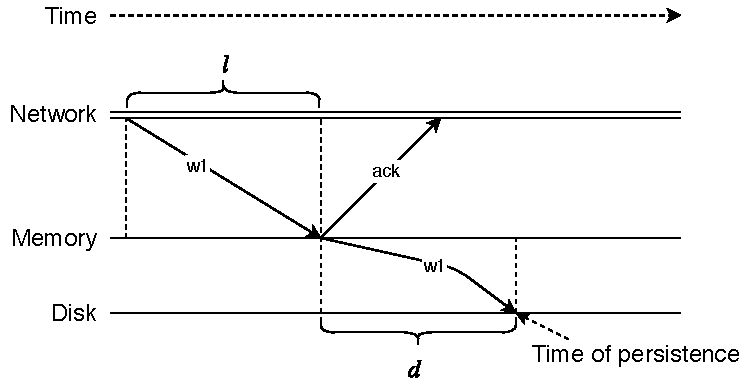
\includegraphics[height=.625\textheight]{../images/write1.pdf} \\
        A write becomes \textit{durable} when it gets \textit{persisted to disk}. \\
        In other words $l + d$.
    \end{center}

\end{frame}

\begin{frame}
    \frametitle{Problem}

    \begin{center}
        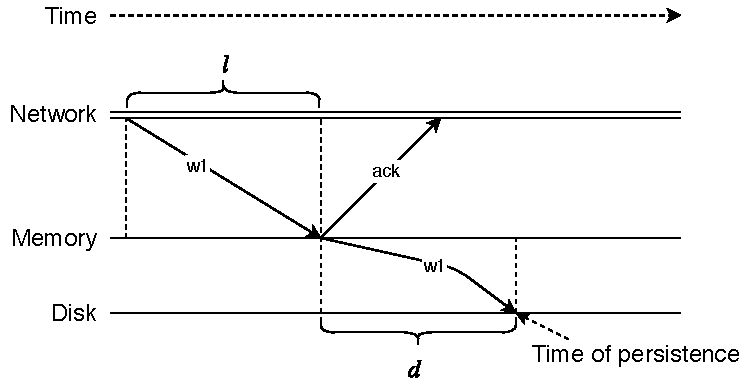
\includegraphics[height=.625\textheight]{../images/write1.pdf} \\
        \textbf{We can't measure $d$.}
    \end{center}

\end{frame}

\begin{frame}
    \frametitle{What can we measure?}

    \begin{itemize}
        \item Latency $l$ (ping)
        \item Response time of write operations... \pause With different \textbf{write concerns}
    \end{itemize}
\end{frame}

\begin{frame}
    \frametitle{Estimating $d$ from Write Concerns}

    Which \textbf{write concern} persists a write to \textit{disk}?
    \pause 

    \textbf{Journaled}!
\end{frame}

\begin{frame}
    \frametitle{Journaled Write Concern}

    A \textbf{Journaled} write will be \textit{applied to memory} and \textit{added to the journal} before being acknowledged. 

    Since the journal does not always hit the disk, we have only an \textit{approximation}.

\end{frame}

\begin{frame}
    \frametitle{Modelling Journaled Write Concern}
    \centering
    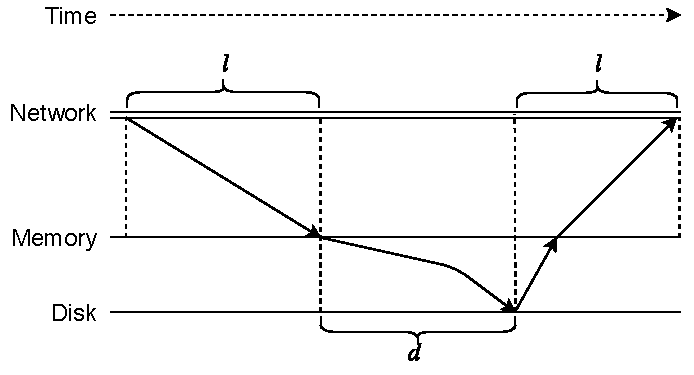
\includegraphics[height=.625\textheight]{../images/j_write.pdf} \\
    Behaviour of a \textbf{Journaled} write.
\end{frame}

\begin{frame}
    \frametitle{Modelling Journaled Write Concern}
    That means, a \textbf{Journaled} write is:
    \[
        j = l + d_{est} + l
    \]
\end{frame}

\begin{frame}
    \frametitle{Estimating durability}

    We want to estimate $t = l + d$ (time to durability).

    We know $l$ and $j = l + d_{est} + l$.

    We then define the \textbf{estimate} as $t_{est} = j - l$:
    \begin{align*}
        t_{est}     &= j - l \\
              &= l + d_{est} \\
              &\approx l + d
    \end{align*}
\end{frame}

\begin{frame}
    \frametitle{Results - latency distribution}

    \begin{figure}
        \centering        
        \scalebox{.5}{%% Creator: Matplotlib, PGF backend
%%
%% To include the figure in your LaTeX document, write
%%   \input{<filename>.pgf}
%%
%% Make sure the required packages are loaded in your preamble
%%   \usepackage{pgf}
%%
%% Figures using additional raster images can only be included by \input if
%% they are in the same directory as the main LaTeX file. For loading figures
%% from other directories you can use the `import` package
%%   \usepackage{import}
%% and then include the figures with
%%   \import{<path to file>}{<filename>.pgf}
%%
%% Matplotlib used the following preamble
%%   \usepackage[utf8x]{inputenc}
%%   \usepackage[T1]{fontenc}
%%   \usepackage{lmodern}
%%
\begingroup%
\makeatletter%
\begin{pgfpicture}%
\pgfpathrectangle{\pgfpointorigin}{\pgfqpoint{6.400000in}{4.800000in}}%
\pgfusepath{use as bounding box, clip}%
\begin{pgfscope}%
\pgfsetbuttcap%
\pgfsetmiterjoin%
\definecolor{currentfill}{rgb}{1.000000,1.000000,1.000000}%
\pgfsetfillcolor{currentfill}%
\pgfsetlinewidth{0.000000pt}%
\definecolor{currentstroke}{rgb}{1.000000,1.000000,1.000000}%
\pgfsetstrokecolor{currentstroke}%
\pgfsetdash{}{0pt}%
\pgfpathmoveto{\pgfqpoint{0.000000in}{0.000000in}}%
\pgfpathlineto{\pgfqpoint{6.400000in}{0.000000in}}%
\pgfpathlineto{\pgfqpoint{6.400000in}{4.800000in}}%
\pgfpathlineto{\pgfqpoint{0.000000in}{4.800000in}}%
\pgfpathclose%
\pgfusepath{fill}%
\end{pgfscope}%
\begin{pgfscope}%
\pgfsetbuttcap%
\pgfsetmiterjoin%
\definecolor{currentfill}{rgb}{1.000000,1.000000,1.000000}%
\pgfsetfillcolor{currentfill}%
\pgfsetlinewidth{0.000000pt}%
\definecolor{currentstroke}{rgb}{0.000000,0.000000,0.000000}%
\pgfsetstrokecolor{currentstroke}%
\pgfsetstrokeopacity{0.000000}%
\pgfsetdash{}{0pt}%
\pgfpathmoveto{\pgfqpoint{0.800000in}{0.528000in}}%
\pgfpathlineto{\pgfqpoint{5.760000in}{0.528000in}}%
\pgfpathlineto{\pgfqpoint{5.760000in}{4.224000in}}%
\pgfpathlineto{\pgfqpoint{0.800000in}{4.224000in}}%
\pgfpathclose%
\pgfusepath{fill}%
\end{pgfscope}%
\begin{pgfscope}%
\pgfsetbuttcap%
\pgfsetroundjoin%
\definecolor{currentfill}{rgb}{0.000000,0.000000,0.000000}%
\pgfsetfillcolor{currentfill}%
\pgfsetlinewidth{0.803000pt}%
\definecolor{currentstroke}{rgb}{0.000000,0.000000,0.000000}%
\pgfsetstrokecolor{currentstroke}%
\pgfsetdash{}{0pt}%
\pgfsys@defobject{currentmarker}{\pgfqpoint{0.000000in}{-0.048611in}}{\pgfqpoint{0.000000in}{0.000000in}}{%
\pgfpathmoveto{\pgfqpoint{0.000000in}{0.000000in}}%
\pgfpathlineto{\pgfqpoint{0.000000in}{-0.048611in}}%
\pgfusepath{stroke,fill}%
}%
\begin{pgfscope}%
\pgfsys@transformshift{1.020936in}{0.528000in}%
\pgfsys@useobject{currentmarker}{}%
\end{pgfscope}%
\end{pgfscope}%
\begin{pgfscope}%
\pgftext[x=1.020936in,y=0.430778in,,top]{\fontsize{11.000000}{13.200000}\selectfont \(\displaystyle 0\)}%
\end{pgfscope}%
\begin{pgfscope}%
\pgfsetbuttcap%
\pgfsetroundjoin%
\definecolor{currentfill}{rgb}{0.000000,0.000000,0.000000}%
\pgfsetfillcolor{currentfill}%
\pgfsetlinewidth{0.803000pt}%
\definecolor{currentstroke}{rgb}{0.000000,0.000000,0.000000}%
\pgfsetstrokecolor{currentstroke}%
\pgfsetdash{}{0pt}%
\pgfsys@defobject{currentmarker}{\pgfqpoint{0.000000in}{-0.048611in}}{\pgfqpoint{0.000000in}{0.000000in}}{%
\pgfpathmoveto{\pgfqpoint{0.000000in}{0.000000in}}%
\pgfpathlineto{\pgfqpoint{0.000000in}{-0.048611in}}%
\pgfusepath{stroke,fill}%
}%
\begin{pgfscope}%
\pgfsys@transformshift{1.924562in}{0.528000in}%
\pgfsys@useobject{currentmarker}{}%
\end{pgfscope}%
\end{pgfscope}%
\begin{pgfscope}%
\pgftext[x=1.924562in,y=0.430778in,,top]{\fontsize{11.000000}{13.200000}\selectfont \(\displaystyle 200\)}%
\end{pgfscope}%
\begin{pgfscope}%
\pgfsetbuttcap%
\pgfsetroundjoin%
\definecolor{currentfill}{rgb}{0.000000,0.000000,0.000000}%
\pgfsetfillcolor{currentfill}%
\pgfsetlinewidth{0.803000pt}%
\definecolor{currentstroke}{rgb}{0.000000,0.000000,0.000000}%
\pgfsetstrokecolor{currentstroke}%
\pgfsetdash{}{0pt}%
\pgfsys@defobject{currentmarker}{\pgfqpoint{0.000000in}{-0.048611in}}{\pgfqpoint{0.000000in}{0.000000in}}{%
\pgfpathmoveto{\pgfqpoint{0.000000in}{0.000000in}}%
\pgfpathlineto{\pgfqpoint{0.000000in}{-0.048611in}}%
\pgfusepath{stroke,fill}%
}%
\begin{pgfscope}%
\pgfsys@transformshift{2.828187in}{0.528000in}%
\pgfsys@useobject{currentmarker}{}%
\end{pgfscope}%
\end{pgfscope}%
\begin{pgfscope}%
\pgftext[x=2.828187in,y=0.430778in,,top]{\fontsize{11.000000}{13.200000}\selectfont \(\displaystyle 400\)}%
\end{pgfscope}%
\begin{pgfscope}%
\pgfsetbuttcap%
\pgfsetroundjoin%
\definecolor{currentfill}{rgb}{0.000000,0.000000,0.000000}%
\pgfsetfillcolor{currentfill}%
\pgfsetlinewidth{0.803000pt}%
\definecolor{currentstroke}{rgb}{0.000000,0.000000,0.000000}%
\pgfsetstrokecolor{currentstroke}%
\pgfsetdash{}{0pt}%
\pgfsys@defobject{currentmarker}{\pgfqpoint{0.000000in}{-0.048611in}}{\pgfqpoint{0.000000in}{0.000000in}}{%
\pgfpathmoveto{\pgfqpoint{0.000000in}{0.000000in}}%
\pgfpathlineto{\pgfqpoint{0.000000in}{-0.048611in}}%
\pgfusepath{stroke,fill}%
}%
\begin{pgfscope}%
\pgfsys@transformshift{3.731813in}{0.528000in}%
\pgfsys@useobject{currentmarker}{}%
\end{pgfscope}%
\end{pgfscope}%
\begin{pgfscope}%
\pgftext[x=3.731813in,y=0.430778in,,top]{\fontsize{11.000000}{13.200000}\selectfont \(\displaystyle 600\)}%
\end{pgfscope}%
\begin{pgfscope}%
\pgfsetbuttcap%
\pgfsetroundjoin%
\definecolor{currentfill}{rgb}{0.000000,0.000000,0.000000}%
\pgfsetfillcolor{currentfill}%
\pgfsetlinewidth{0.803000pt}%
\definecolor{currentstroke}{rgb}{0.000000,0.000000,0.000000}%
\pgfsetstrokecolor{currentstroke}%
\pgfsetdash{}{0pt}%
\pgfsys@defobject{currentmarker}{\pgfqpoint{0.000000in}{-0.048611in}}{\pgfqpoint{0.000000in}{0.000000in}}{%
\pgfpathmoveto{\pgfqpoint{0.000000in}{0.000000in}}%
\pgfpathlineto{\pgfqpoint{0.000000in}{-0.048611in}}%
\pgfusepath{stroke,fill}%
}%
\begin{pgfscope}%
\pgfsys@transformshift{4.635438in}{0.528000in}%
\pgfsys@useobject{currentmarker}{}%
\end{pgfscope}%
\end{pgfscope}%
\begin{pgfscope}%
\pgftext[x=4.635438in,y=0.430778in,,top]{\fontsize{11.000000}{13.200000}\selectfont \(\displaystyle 800\)}%
\end{pgfscope}%
\begin{pgfscope}%
\pgfsetbuttcap%
\pgfsetroundjoin%
\definecolor{currentfill}{rgb}{0.000000,0.000000,0.000000}%
\pgfsetfillcolor{currentfill}%
\pgfsetlinewidth{0.803000pt}%
\definecolor{currentstroke}{rgb}{0.000000,0.000000,0.000000}%
\pgfsetstrokecolor{currentstroke}%
\pgfsetdash{}{0pt}%
\pgfsys@defobject{currentmarker}{\pgfqpoint{0.000000in}{-0.048611in}}{\pgfqpoint{0.000000in}{0.000000in}}{%
\pgfpathmoveto{\pgfqpoint{0.000000in}{0.000000in}}%
\pgfpathlineto{\pgfqpoint{0.000000in}{-0.048611in}}%
\pgfusepath{stroke,fill}%
}%
\begin{pgfscope}%
\pgfsys@transformshift{5.539064in}{0.528000in}%
\pgfsys@useobject{currentmarker}{}%
\end{pgfscope}%
\end{pgfscope}%
\begin{pgfscope}%
\pgftext[x=5.539064in,y=0.430778in,,top]{\fontsize{11.000000}{13.200000}\selectfont \(\displaystyle 1000\)}%
\end{pgfscope}%
\begin{pgfscope}%
\pgftext[x=3.280000in,y=0.240271in,,top]{\fontsize{11.000000}{13.200000}\selectfont Latency (in milliseconds)}%
\end{pgfscope}%
\begin{pgfscope}%
\pgfsetbuttcap%
\pgfsetroundjoin%
\definecolor{currentfill}{rgb}{0.000000,0.000000,0.000000}%
\pgfsetfillcolor{currentfill}%
\pgfsetlinewidth{0.803000pt}%
\definecolor{currentstroke}{rgb}{0.000000,0.000000,0.000000}%
\pgfsetstrokecolor{currentstroke}%
\pgfsetdash{}{0pt}%
\pgfsys@defobject{currentmarker}{\pgfqpoint{-0.048611in}{0.000000in}}{\pgfqpoint{0.000000in}{0.000000in}}{%
\pgfpathmoveto{\pgfqpoint{0.000000in}{0.000000in}}%
\pgfpathlineto{\pgfqpoint{-0.048611in}{0.000000in}}%
\pgfusepath{stroke,fill}%
}%
\begin{pgfscope}%
\pgfsys@transformshift{0.800000in}{0.696000in}%
\pgfsys@useobject{currentmarker}{}%
\end{pgfscope}%
\end{pgfscope}%
\begin{pgfscope}%
\pgftext[x=0.627981in,y=0.643378in,left,base]{\fontsize{11.000000}{13.200000}\selectfont \(\displaystyle 0\)}%
\end{pgfscope}%
\begin{pgfscope}%
\pgfsetbuttcap%
\pgfsetroundjoin%
\definecolor{currentfill}{rgb}{0.000000,0.000000,0.000000}%
\pgfsetfillcolor{currentfill}%
\pgfsetlinewidth{0.803000pt}%
\definecolor{currentstroke}{rgb}{0.000000,0.000000,0.000000}%
\pgfsetstrokecolor{currentstroke}%
\pgfsetdash{}{0pt}%
\pgfsys@defobject{currentmarker}{\pgfqpoint{-0.048611in}{0.000000in}}{\pgfqpoint{0.000000in}{0.000000in}}{%
\pgfpathmoveto{\pgfqpoint{0.000000in}{0.000000in}}%
\pgfpathlineto{\pgfqpoint{-0.048611in}{0.000000in}}%
\pgfusepath{stroke,fill}%
}%
\begin{pgfscope}%
\pgfsys@transformshift{0.800000in}{1.129492in}%
\pgfsys@useobject{currentmarker}{}%
\end{pgfscope}%
\end{pgfscope}%
\begin{pgfscope}%
\pgftext[x=0.403588in,y=1.076870in,left,base]{\fontsize{11.000000}{13.200000}\selectfont \(\displaystyle 1000\)}%
\end{pgfscope}%
\begin{pgfscope}%
\pgfsetbuttcap%
\pgfsetroundjoin%
\definecolor{currentfill}{rgb}{0.000000,0.000000,0.000000}%
\pgfsetfillcolor{currentfill}%
\pgfsetlinewidth{0.803000pt}%
\definecolor{currentstroke}{rgb}{0.000000,0.000000,0.000000}%
\pgfsetstrokecolor{currentstroke}%
\pgfsetdash{}{0pt}%
\pgfsys@defobject{currentmarker}{\pgfqpoint{-0.048611in}{0.000000in}}{\pgfqpoint{0.000000in}{0.000000in}}{%
\pgfpathmoveto{\pgfqpoint{0.000000in}{0.000000in}}%
\pgfpathlineto{\pgfqpoint{-0.048611in}{0.000000in}}%
\pgfusepath{stroke,fill}%
}%
\begin{pgfscope}%
\pgfsys@transformshift{0.800000in}{1.562985in}%
\pgfsys@useobject{currentmarker}{}%
\end{pgfscope}%
\end{pgfscope}%
\begin{pgfscope}%
\pgftext[x=0.403588in,y=1.510363in,left,base]{\fontsize{11.000000}{13.200000}\selectfont \(\displaystyle 2000\)}%
\end{pgfscope}%
\begin{pgfscope}%
\pgfsetbuttcap%
\pgfsetroundjoin%
\definecolor{currentfill}{rgb}{0.000000,0.000000,0.000000}%
\pgfsetfillcolor{currentfill}%
\pgfsetlinewidth{0.803000pt}%
\definecolor{currentstroke}{rgb}{0.000000,0.000000,0.000000}%
\pgfsetstrokecolor{currentstroke}%
\pgfsetdash{}{0pt}%
\pgfsys@defobject{currentmarker}{\pgfqpoint{-0.048611in}{0.000000in}}{\pgfqpoint{0.000000in}{0.000000in}}{%
\pgfpathmoveto{\pgfqpoint{0.000000in}{0.000000in}}%
\pgfpathlineto{\pgfqpoint{-0.048611in}{0.000000in}}%
\pgfusepath{stroke,fill}%
}%
\begin{pgfscope}%
\pgfsys@transformshift{0.800000in}{1.996477in}%
\pgfsys@useobject{currentmarker}{}%
\end{pgfscope}%
\end{pgfscope}%
\begin{pgfscope}%
\pgftext[x=0.403588in,y=1.943855in,left,base]{\fontsize{11.000000}{13.200000}\selectfont \(\displaystyle 3000\)}%
\end{pgfscope}%
\begin{pgfscope}%
\pgfsetbuttcap%
\pgfsetroundjoin%
\definecolor{currentfill}{rgb}{0.000000,0.000000,0.000000}%
\pgfsetfillcolor{currentfill}%
\pgfsetlinewidth{0.803000pt}%
\definecolor{currentstroke}{rgb}{0.000000,0.000000,0.000000}%
\pgfsetstrokecolor{currentstroke}%
\pgfsetdash{}{0pt}%
\pgfsys@defobject{currentmarker}{\pgfqpoint{-0.048611in}{0.000000in}}{\pgfqpoint{0.000000in}{0.000000in}}{%
\pgfpathmoveto{\pgfqpoint{0.000000in}{0.000000in}}%
\pgfpathlineto{\pgfqpoint{-0.048611in}{0.000000in}}%
\pgfusepath{stroke,fill}%
}%
\begin{pgfscope}%
\pgfsys@transformshift{0.800000in}{2.429970in}%
\pgfsys@useobject{currentmarker}{}%
\end{pgfscope}%
\end{pgfscope}%
\begin{pgfscope}%
\pgftext[x=0.403588in,y=2.377348in,left,base]{\fontsize{11.000000}{13.200000}\selectfont \(\displaystyle 4000\)}%
\end{pgfscope}%
\begin{pgfscope}%
\pgfsetbuttcap%
\pgfsetroundjoin%
\definecolor{currentfill}{rgb}{0.000000,0.000000,0.000000}%
\pgfsetfillcolor{currentfill}%
\pgfsetlinewidth{0.803000pt}%
\definecolor{currentstroke}{rgb}{0.000000,0.000000,0.000000}%
\pgfsetstrokecolor{currentstroke}%
\pgfsetdash{}{0pt}%
\pgfsys@defobject{currentmarker}{\pgfqpoint{-0.048611in}{0.000000in}}{\pgfqpoint{0.000000in}{0.000000in}}{%
\pgfpathmoveto{\pgfqpoint{0.000000in}{0.000000in}}%
\pgfpathlineto{\pgfqpoint{-0.048611in}{0.000000in}}%
\pgfusepath{stroke,fill}%
}%
\begin{pgfscope}%
\pgfsys@transformshift{0.800000in}{2.863462in}%
\pgfsys@useobject{currentmarker}{}%
\end{pgfscope}%
\end{pgfscope}%
\begin{pgfscope}%
\pgftext[x=0.403588in,y=2.810840in,left,base]{\fontsize{11.000000}{13.200000}\selectfont \(\displaystyle 5000\)}%
\end{pgfscope}%
\begin{pgfscope}%
\pgfsetbuttcap%
\pgfsetroundjoin%
\definecolor{currentfill}{rgb}{0.000000,0.000000,0.000000}%
\pgfsetfillcolor{currentfill}%
\pgfsetlinewidth{0.803000pt}%
\definecolor{currentstroke}{rgb}{0.000000,0.000000,0.000000}%
\pgfsetstrokecolor{currentstroke}%
\pgfsetdash{}{0pt}%
\pgfsys@defobject{currentmarker}{\pgfqpoint{-0.048611in}{0.000000in}}{\pgfqpoint{0.000000in}{0.000000in}}{%
\pgfpathmoveto{\pgfqpoint{0.000000in}{0.000000in}}%
\pgfpathlineto{\pgfqpoint{-0.048611in}{0.000000in}}%
\pgfusepath{stroke,fill}%
}%
\begin{pgfscope}%
\pgfsys@transformshift{0.800000in}{3.296955in}%
\pgfsys@useobject{currentmarker}{}%
\end{pgfscope}%
\end{pgfscope}%
\begin{pgfscope}%
\pgftext[x=0.403588in,y=3.244332in,left,base]{\fontsize{11.000000}{13.200000}\selectfont \(\displaystyle 6000\)}%
\end{pgfscope}%
\begin{pgfscope}%
\pgfsetbuttcap%
\pgfsetroundjoin%
\definecolor{currentfill}{rgb}{0.000000,0.000000,0.000000}%
\pgfsetfillcolor{currentfill}%
\pgfsetlinewidth{0.803000pt}%
\definecolor{currentstroke}{rgb}{0.000000,0.000000,0.000000}%
\pgfsetstrokecolor{currentstroke}%
\pgfsetdash{}{0pt}%
\pgfsys@defobject{currentmarker}{\pgfqpoint{-0.048611in}{0.000000in}}{\pgfqpoint{0.000000in}{0.000000in}}{%
\pgfpathmoveto{\pgfqpoint{0.000000in}{0.000000in}}%
\pgfpathlineto{\pgfqpoint{-0.048611in}{0.000000in}}%
\pgfusepath{stroke,fill}%
}%
\begin{pgfscope}%
\pgfsys@transformshift{0.800000in}{3.730447in}%
\pgfsys@useobject{currentmarker}{}%
\end{pgfscope}%
\end{pgfscope}%
\begin{pgfscope}%
\pgftext[x=0.403588in,y=3.677825in,left,base]{\fontsize{11.000000}{13.200000}\selectfont \(\displaystyle 7000\)}%
\end{pgfscope}%
\begin{pgfscope}%
\pgfsetbuttcap%
\pgfsetroundjoin%
\definecolor{currentfill}{rgb}{0.000000,0.000000,0.000000}%
\pgfsetfillcolor{currentfill}%
\pgfsetlinewidth{0.803000pt}%
\definecolor{currentstroke}{rgb}{0.000000,0.000000,0.000000}%
\pgfsetstrokecolor{currentstroke}%
\pgfsetdash{}{0pt}%
\pgfsys@defobject{currentmarker}{\pgfqpoint{-0.048611in}{0.000000in}}{\pgfqpoint{0.000000in}{0.000000in}}{%
\pgfpathmoveto{\pgfqpoint{0.000000in}{0.000000in}}%
\pgfpathlineto{\pgfqpoint{-0.048611in}{0.000000in}}%
\pgfusepath{stroke,fill}%
}%
\begin{pgfscope}%
\pgfsys@transformshift{0.800000in}{4.163940in}%
\pgfsys@useobject{currentmarker}{}%
\end{pgfscope}%
\end{pgfscope}%
\begin{pgfscope}%
\pgftext[x=0.403588in,y=4.111317in,left,base]{\fontsize{11.000000}{13.200000}\selectfont \(\displaystyle 8000\)}%
\end{pgfscope}%
\begin{pgfscope}%
\pgftext[x=0.348033in,y=2.376000in,,bottom,rotate=90.000000]{\fontsize{11.000000}{13.200000}\selectfont Number of operations}%
\end{pgfscope}%
\begin{pgfscope}%
\pgfpathrectangle{\pgfqpoint{0.800000in}{0.528000in}}{\pgfqpoint{4.960000in}{3.696000in}}%
\pgfusepath{clip}%
\pgfsetrectcap%
\pgfsetroundjoin%
\pgfsetlinewidth{1.505625pt}%
\definecolor{currentstroke}{rgb}{0.121569,0.466667,0.705882}%
\pgfsetstrokecolor{currentstroke}%
\pgfsetdash{}{0pt}%
\pgfpathmoveto{\pgfqpoint{1.025455in}{1.752855in}}%
\pgfpathlineto{\pgfqpoint{1.029973in}{1.641447in}}%
\pgfpathlineto{\pgfqpoint{1.034491in}{1.632344in}}%
\pgfpathlineto{\pgfqpoint{1.039009in}{1.615871in}}%
\pgfpathlineto{\pgfqpoint{1.043527in}{1.570788in}}%
\pgfpathlineto{\pgfqpoint{1.048045in}{1.623674in}}%
\pgfpathlineto{\pgfqpoint{1.052563in}{1.613270in}}%
\pgfpathlineto{\pgfqpoint{1.061600in}{1.502296in}}%
\pgfpathlineto{\pgfqpoint{1.066118in}{1.454178in}}%
\pgfpathlineto{\pgfqpoint{1.070636in}{1.436839in}}%
\pgfpathlineto{\pgfqpoint{1.075154in}{1.357943in}}%
\pgfpathlineto{\pgfqpoint{1.079672in}{1.379184in}}%
\pgfpathlineto{\pgfqpoint{1.084190in}{1.332367in}}%
\pgfpathlineto{\pgfqpoint{1.097745in}{1.240467in}}%
\pgfpathlineto{\pgfqpoint{1.102263in}{1.184979in}}%
\pgfpathlineto{\pgfqpoint{1.106781in}{1.148133in}}%
\pgfpathlineto{\pgfqpoint{1.111299in}{1.142064in}}%
\pgfpathlineto{\pgfqpoint{1.115817in}{1.080941in}}%
\pgfpathlineto{\pgfqpoint{1.120335in}{1.077473in}}%
\pgfpathlineto{\pgfqpoint{1.124853in}{1.051897in}}%
\pgfpathlineto{\pgfqpoint{1.129371in}{1.044961in}}%
\pgfpathlineto{\pgfqpoint{1.133890in}{1.019819in}}%
\pgfpathlineto{\pgfqpoint{1.138408in}{1.002479in}}%
\pgfpathlineto{\pgfqpoint{1.147444in}{0.945692in}}%
\pgfpathlineto{\pgfqpoint{1.151962in}{0.924451in}}%
\pgfpathlineto{\pgfqpoint{1.156480in}{0.941790in}}%
\pgfpathlineto{\pgfqpoint{1.160998in}{0.890638in}}%
\pgfpathlineto{\pgfqpoint{1.165516in}{0.902342in}}%
\pgfpathlineto{\pgfqpoint{1.174553in}{0.842087in}}%
\pgfpathlineto{\pgfqpoint{1.179071in}{0.838186in}}%
\pgfpathlineto{\pgfqpoint{1.183589in}{0.841220in}}%
\pgfpathlineto{\pgfqpoint{1.188107in}{0.829082in}}%
\pgfpathlineto{\pgfqpoint{1.192625in}{0.837752in}}%
\pgfpathlineto{\pgfqpoint{1.197143in}{0.825181in}}%
\pgfpathlineto{\pgfqpoint{1.201662in}{0.835151in}}%
\pgfpathlineto{\pgfqpoint{1.206180in}{0.827782in}}%
\pgfpathlineto{\pgfqpoint{1.210698in}{0.845988in}}%
\pgfpathlineto{\pgfqpoint{1.215216in}{0.857693in}}%
\pgfpathlineto{\pgfqpoint{1.219734in}{0.886303in}}%
\pgfpathlineto{\pgfqpoint{1.224252in}{0.924451in}}%
\pgfpathlineto{\pgfqpoint{1.228770in}{0.944825in}}%
\pgfpathlineto{\pgfqpoint{1.237807in}{1.063602in}}%
\pgfpathlineto{\pgfqpoint{1.242325in}{1.126025in}}%
\pgfpathlineto{\pgfqpoint{1.246843in}{1.347973in}}%
\pgfpathlineto{\pgfqpoint{1.251361in}{1.315461in}}%
\pgfpathlineto{\pgfqpoint{1.255879in}{1.435105in}}%
\pgfpathlineto{\pgfqpoint{1.260397in}{1.496661in}}%
\pgfpathlineto{\pgfqpoint{1.264915in}{1.742884in}}%
\pgfpathlineto{\pgfqpoint{1.273952in}{2.383153in}}%
\pgfpathlineto{\pgfqpoint{1.278470in}{2.811877in}}%
\pgfpathlineto{\pgfqpoint{1.282988in}{2.925018in}}%
\pgfpathlineto{\pgfqpoint{1.287506in}{2.944959in}}%
\pgfpathlineto{\pgfqpoint{1.292024in}{3.285684in}}%
\pgfpathlineto{\pgfqpoint{1.296542in}{3.500696in}}%
\pgfpathlineto{\pgfqpoint{1.301060in}{3.795471in}}%
\pgfpathlineto{\pgfqpoint{1.305578in}{3.819747in}}%
\pgfpathlineto{\pgfqpoint{1.310097in}{3.826249in}}%
\pgfpathlineto{\pgfqpoint{1.314615in}{4.056000in}}%
\pgfpathlineto{\pgfqpoint{1.319133in}{3.809343in}}%
\pgfpathlineto{\pgfqpoint{1.323651in}{3.720477in}}%
\pgfpathlineto{\pgfqpoint{1.328169in}{3.785934in}}%
\pgfpathlineto{\pgfqpoint{1.332687in}{3.953262in}}%
\pgfpathlineto{\pgfqpoint{1.337205in}{4.017853in}}%
\pgfpathlineto{\pgfqpoint{1.341723in}{4.033458in}}%
\pgfpathlineto{\pgfqpoint{1.346242in}{3.977104in}}%
\pgfpathlineto{\pgfqpoint{1.355278in}{3.625975in}}%
\pgfpathlineto{\pgfqpoint{1.359796in}{3.322097in}}%
\pgfpathlineto{\pgfqpoint{1.364314in}{3.151735in}}%
\pgfpathlineto{\pgfqpoint{1.368832in}{2.882969in}}%
\pgfpathlineto{\pgfqpoint{1.391423in}{2.148200in}}%
\pgfpathlineto{\pgfqpoint{1.400459in}{1.983906in}}%
\pgfpathlineto{\pgfqpoint{1.404977in}{1.849957in}}%
\pgfpathlineto{\pgfqpoint{1.414013in}{1.676993in}}%
\pgfpathlineto{\pgfqpoint{1.423050in}{1.565152in}}%
\pgfpathlineto{\pgfqpoint{1.427568in}{1.466316in}}%
\pgfpathlineto{\pgfqpoint{1.432086in}{1.421666in}}%
\pgfpathlineto{\pgfqpoint{1.436604in}{1.327599in}}%
\pgfpathlineto{\pgfqpoint{1.441122in}{1.269077in}}%
\pgfpathlineto{\pgfqpoint{1.445640in}{1.277747in}}%
\pgfpathlineto{\pgfqpoint{1.450158in}{1.276013in}}%
\pgfpathlineto{\pgfqpoint{1.454677in}{1.243067in}}%
\pgfpathlineto{\pgfqpoint{1.459195in}{1.229629in}}%
\pgfpathlineto{\pgfqpoint{1.463713in}{1.184979in}}%
\pgfpathlineto{\pgfqpoint{1.468231in}{1.108251in}}%
\pgfpathlineto{\pgfqpoint{1.472749in}{1.091345in}}%
\pgfpathlineto{\pgfqpoint{1.477267in}{1.093513in}}%
\pgfpathlineto{\pgfqpoint{1.481785in}{1.081375in}}%
\pgfpathlineto{\pgfqpoint{1.490822in}{0.973435in}}%
\pgfpathlineto{\pgfqpoint{1.495340in}{0.980371in}}%
\pgfpathlineto{\pgfqpoint{1.499858in}{1.012016in}}%
\pgfpathlineto{\pgfqpoint{1.504376in}{0.963898in}}%
\pgfpathlineto{\pgfqpoint{1.508894in}{0.977337in}}%
\pgfpathlineto{\pgfqpoint{1.513412in}{1.004647in}}%
\pgfpathlineto{\pgfqpoint{1.517930in}{1.020252in}}%
\pgfpathlineto{\pgfqpoint{1.522449in}{1.025454in}}%
\pgfpathlineto{\pgfqpoint{1.526967in}{1.078774in}}%
\pgfpathlineto{\pgfqpoint{1.531485in}{1.110852in}}%
\pgfpathlineto{\pgfqpoint{1.536003in}{1.189748in}}%
\pgfpathlineto{\pgfqpoint{1.540521in}{1.138162in}}%
\pgfpathlineto{\pgfqpoint{1.545039in}{1.237432in}}%
\pgfpathlineto{\pgfqpoint{1.554075in}{1.305057in}}%
\pgfpathlineto{\pgfqpoint{1.558594in}{1.378317in}}%
\pgfpathlineto{\pgfqpoint{1.563112in}{1.471951in}}%
\pgfpathlineto{\pgfqpoint{1.567630in}{1.603300in}}%
\pgfpathlineto{\pgfqpoint{1.572148in}{1.550847in}}%
\pgfpathlineto{\pgfqpoint{1.576666in}{1.672658in}}%
\pgfpathlineto{\pgfqpoint{1.581184in}{1.702136in}}%
\pgfpathlineto{\pgfqpoint{1.585702in}{1.791435in}}%
\pgfpathlineto{\pgfqpoint{1.590220in}{1.761091in}}%
\pgfpathlineto{\pgfqpoint{1.599257in}{1.924084in}}%
\pgfpathlineto{\pgfqpoint{1.612811in}{2.146899in}}%
\pgfpathlineto{\pgfqpoint{1.617329in}{2.258307in}}%
\pgfpathlineto{\pgfqpoint{1.621847in}{2.423467in}}%
\pgfpathlineto{\pgfqpoint{1.626365in}{2.496294in}}%
\pgfpathlineto{\pgfqpoint{1.630884in}{2.638480in}}%
\pgfpathlineto{\pgfqpoint{1.635402in}{2.709572in}}%
\pgfpathlineto{\pgfqpoint{1.639920in}{2.857827in}}%
\pgfpathlineto{\pgfqpoint{1.644438in}{2.914181in}}%
\pgfpathlineto{\pgfqpoint{1.648956in}{3.095814in}}%
\pgfpathlineto{\pgfqpoint{1.653474in}{2.964033in}}%
\pgfpathlineto{\pgfqpoint{1.657992in}{3.016485in}}%
\pgfpathlineto{\pgfqpoint{1.662510in}{3.015185in}}%
\pgfpathlineto{\pgfqpoint{1.667029in}{2.932821in}}%
\pgfpathlineto{\pgfqpoint{1.671547in}{2.747286in}}%
\pgfpathlineto{\pgfqpoint{1.676065in}{2.692233in}}%
\pgfpathlineto{\pgfqpoint{1.685101in}{2.489792in}}%
\pgfpathlineto{\pgfqpoint{1.689619in}{2.528373in}}%
\pgfpathlineto{\pgfqpoint{1.694137in}{2.403527in}}%
\pgfpathlineto{\pgfqpoint{1.698655in}{2.352808in}}%
\pgfpathlineto{\pgfqpoint{1.703174in}{2.323764in}}%
\pgfpathlineto{\pgfqpoint{1.707692in}{2.322464in}}%
\pgfpathlineto{\pgfqpoint{1.716728in}{2.035925in}}%
\pgfpathlineto{\pgfqpoint{1.721246in}{2.004280in}}%
\pgfpathlineto{\pgfqpoint{1.725764in}{1.848656in}}%
\pgfpathlineto{\pgfqpoint{1.730282in}{1.737249in}}%
\pgfpathlineto{\pgfqpoint{1.734801in}{1.731180in}}%
\pgfpathlineto{\pgfqpoint{1.739319in}{1.646215in}}%
\pgfpathlineto{\pgfqpoint{1.748355in}{1.534808in}}%
\pgfpathlineto{\pgfqpoint{1.752873in}{1.513133in}}%
\pgfpathlineto{\pgfqpoint{1.757391in}{1.441607in}}%
\pgfpathlineto{\pgfqpoint{1.766427in}{1.376583in}}%
\pgfpathlineto{\pgfqpoint{1.770946in}{1.371815in}}%
\pgfpathlineto{\pgfqpoint{1.775464in}{1.348406in}}%
\pgfpathlineto{\pgfqpoint{1.779982in}{1.292919in}}%
\pgfpathlineto{\pgfqpoint{1.784500in}{1.255205in}}%
\pgfpathlineto{\pgfqpoint{1.789018in}{1.234831in}}%
\pgfpathlineto{\pgfqpoint{1.793536in}{1.250870in}}%
\pgfpathlineto{\pgfqpoint{1.798054in}{1.214890in}}%
\pgfpathlineto{\pgfqpoint{1.802572in}{1.282949in}}%
\pgfpathlineto{\pgfqpoint{1.807091in}{1.157669in}}%
\pgfpathlineto{\pgfqpoint{1.811609in}{1.167206in}}%
\pgfpathlineto{\pgfqpoint{1.820645in}{1.200585in}}%
\pgfpathlineto{\pgfqpoint{1.825163in}{1.212290in}}%
\pgfpathlineto{\pgfqpoint{1.829681in}{1.228762in}}%
\pgfpathlineto{\pgfqpoint{1.834199in}{1.258240in}}%
\pgfpathlineto{\pgfqpoint{1.838717in}{1.209689in}}%
\pgfpathlineto{\pgfqpoint{1.843236in}{1.213156in}}%
\pgfpathlineto{\pgfqpoint{1.847754in}{1.293353in}}%
\pgfpathlineto{\pgfqpoint{1.852272in}{1.214890in}}%
\pgfpathlineto{\pgfqpoint{1.856790in}{1.219225in}}%
\pgfpathlineto{\pgfqpoint{1.861308in}{1.263008in}}%
\pgfpathlineto{\pgfqpoint{1.865826in}{1.239166in}}%
\pgfpathlineto{\pgfqpoint{1.870344in}{1.230063in}}%
\pgfpathlineto{\pgfqpoint{1.874862in}{1.254338in}}%
\pgfpathlineto{\pgfqpoint{1.879381in}{1.372248in}}%
\pgfpathlineto{\pgfqpoint{1.883899in}{1.419499in}}%
\pgfpathlineto{\pgfqpoint{1.888417in}{1.355342in}}%
\pgfpathlineto{\pgfqpoint{1.892935in}{1.405194in}}%
\pgfpathlineto{\pgfqpoint{1.897453in}{1.474552in}}%
\pgfpathlineto{\pgfqpoint{1.901971in}{1.505764in}}%
\pgfpathlineto{\pgfqpoint{1.906489in}{1.510532in}}%
\pgfpathlineto{\pgfqpoint{1.911007in}{1.559950in}}%
\pgfpathlineto{\pgfqpoint{1.915526in}{1.534808in}}%
\pgfpathlineto{\pgfqpoint{1.920044in}{1.527005in}}%
\pgfpathlineto{\pgfqpoint{1.924562in}{1.527872in}}%
\pgfpathlineto{\pgfqpoint{1.929080in}{1.539576in}}%
\pgfpathlineto{\pgfqpoint{1.933598in}{1.578157in}}%
\pgfpathlineto{\pgfqpoint{1.938116in}{1.629743in}}%
\pgfpathlineto{\pgfqpoint{1.942634in}{1.619339in}}%
\pgfpathlineto{\pgfqpoint{1.947152in}{1.644915in}}%
\pgfpathlineto{\pgfqpoint{1.951671in}{1.618905in}}%
\pgfpathlineto{\pgfqpoint{1.956189in}{1.713840in}}%
\pgfpathlineto{\pgfqpoint{1.960707in}{1.715574in}}%
\pgfpathlineto{\pgfqpoint{1.965225in}{1.683929in}}%
\pgfpathlineto{\pgfqpoint{1.969743in}{1.739416in}}%
\pgfpathlineto{\pgfqpoint{1.974261in}{1.658353in}}%
\pgfpathlineto{\pgfqpoint{1.978779in}{1.670925in}}%
\pgfpathlineto{\pgfqpoint{1.983298in}{1.674392in}}%
\pgfpathlineto{\pgfqpoint{1.987816in}{1.630176in}}%
\pgfpathlineto{\pgfqpoint{1.992334in}{1.604600in}}%
\pgfpathlineto{\pgfqpoint{1.996852in}{1.597664in}}%
\pgfpathlineto{\pgfqpoint{2.001370in}{1.546512in}}%
\pgfpathlineto{\pgfqpoint{2.005888in}{1.535675in}}%
\pgfpathlineto{\pgfqpoint{2.010406in}{1.495794in}}%
\pgfpathlineto{\pgfqpoint{2.014924in}{1.471085in}}%
\pgfpathlineto{\pgfqpoint{2.019443in}{1.459814in}}%
\pgfpathlineto{\pgfqpoint{2.023961in}{1.429469in}}%
\pgfpathlineto{\pgfqpoint{2.028479in}{1.416031in}}%
\pgfpathlineto{\pgfqpoint{2.032997in}{1.307224in}}%
\pgfpathlineto{\pgfqpoint{2.037515in}{1.298121in}}%
\pgfpathlineto{\pgfqpoint{2.042033in}{1.270811in}}%
\pgfpathlineto{\pgfqpoint{2.046551in}{1.305057in}}%
\pgfpathlineto{\pgfqpoint{2.055588in}{1.193216in}}%
\pgfpathlineto{\pgfqpoint{2.060106in}{1.197551in}}%
\pgfpathlineto{\pgfqpoint{2.064624in}{1.167640in}}%
\pgfpathlineto{\pgfqpoint{2.069142in}{1.180211in}}%
\pgfpathlineto{\pgfqpoint{2.078178in}{1.181078in}}%
\pgfpathlineto{\pgfqpoint{2.082696in}{1.118222in}}%
\pgfpathlineto{\pgfqpoint{2.087214in}{1.116921in}}%
\pgfpathlineto{\pgfqpoint{2.096251in}{1.060567in}}%
\pgfpathlineto{\pgfqpoint{2.100769in}{1.091345in}}%
\pgfpathlineto{\pgfqpoint{2.105287in}{1.045828in}}%
\pgfpathlineto{\pgfqpoint{2.109805in}{1.063168in}}%
\pgfpathlineto{\pgfqpoint{2.118841in}{1.065769in}}%
\pgfpathlineto{\pgfqpoint{2.123359in}{1.065769in}}%
\pgfpathlineto{\pgfqpoint{2.127878in}{1.069670in}}%
\pgfpathlineto{\pgfqpoint{2.132396in}{1.080508in}}%
\pgfpathlineto{\pgfqpoint{2.136914in}{1.110852in}}%
\pgfpathlineto{\pgfqpoint{2.141432in}{1.132527in}}%
\pgfpathlineto{\pgfqpoint{2.145950in}{1.087877in}}%
\pgfpathlineto{\pgfqpoint{2.150468in}{1.098281in}}%
\pgfpathlineto{\pgfqpoint{2.154986in}{1.043661in}}%
\pgfpathlineto{\pgfqpoint{2.159504in}{1.046262in}}%
\pgfpathlineto{\pgfqpoint{2.164023in}{1.050597in}}%
\pgfpathlineto{\pgfqpoint{2.168541in}{1.042360in}}%
\pgfpathlineto{\pgfqpoint{2.173059in}{1.054065in}}%
\pgfpathlineto{\pgfqpoint{2.177577in}{1.044094in}}%
\pgfpathlineto{\pgfqpoint{2.182095in}{1.062735in}}%
\pgfpathlineto{\pgfqpoint{2.186613in}{1.045828in}}%
\pgfpathlineto{\pgfqpoint{2.191131in}{1.065336in}}%
\pgfpathlineto{\pgfqpoint{2.195649in}{1.025888in}}%
\pgfpathlineto{\pgfqpoint{2.200168in}{1.018518in}}%
\pgfpathlineto{\pgfqpoint{2.209204in}{1.017651in}}%
\pgfpathlineto{\pgfqpoint{2.213722in}{1.010282in}}%
\pgfpathlineto{\pgfqpoint{2.218240in}{0.992509in}}%
\pgfpathlineto{\pgfqpoint{2.222758in}{1.012449in}}%
\pgfpathlineto{\pgfqpoint{2.227276in}{1.044528in}}%
\pgfpathlineto{\pgfqpoint{2.231794in}{1.058833in}}%
\pgfpathlineto{\pgfqpoint{2.236313in}{1.053631in}}%
\pgfpathlineto{\pgfqpoint{2.240831in}{1.053631in}}%
\pgfpathlineto{\pgfqpoint{2.245349in}{1.078340in}}%
\pgfpathlineto{\pgfqpoint{2.249867in}{1.061868in}}%
\pgfpathlineto{\pgfqpoint{2.254385in}{1.104783in}}%
\pgfpathlineto{\pgfqpoint{2.258903in}{1.101315in}}%
\pgfpathlineto{\pgfqpoint{2.263421in}{1.121256in}}%
\pgfpathlineto{\pgfqpoint{2.267940in}{1.091345in}}%
\pgfpathlineto{\pgfqpoint{2.272458in}{1.104350in}}%
\pgfpathlineto{\pgfqpoint{2.276976in}{1.075739in}}%
\pgfpathlineto{\pgfqpoint{2.281494in}{1.073138in}}%
\pgfpathlineto{\pgfqpoint{2.286012in}{1.079641in}}%
\pgfpathlineto{\pgfqpoint{2.290530in}{1.070537in}}%
\pgfpathlineto{\pgfqpoint{2.295048in}{1.037592in}}%
\pgfpathlineto{\pgfqpoint{2.299566in}{1.016351in}}%
\pgfpathlineto{\pgfqpoint{2.304085in}{1.087010in}}%
\pgfpathlineto{\pgfqpoint{2.308603in}{1.055799in}}%
\pgfpathlineto{\pgfqpoint{2.313121in}{1.049296in}}%
\pgfpathlineto{\pgfqpoint{2.317639in}{1.044961in}}%
\pgfpathlineto{\pgfqpoint{2.322157in}{1.050597in}}%
\pgfpathlineto{\pgfqpoint{2.331193in}{0.992509in}}%
\pgfpathlineto{\pgfqpoint{2.335711in}{0.999445in}}%
\pgfpathlineto{\pgfqpoint{2.340230in}{0.978637in}}%
\pgfpathlineto{\pgfqpoint{2.344748in}{0.994676in}}%
\pgfpathlineto{\pgfqpoint{2.353784in}{0.953928in}}%
\pgfpathlineto{\pgfqpoint{2.358302in}{0.948293in}}%
\pgfpathlineto{\pgfqpoint{2.362820in}{1.014617in}}%
\pgfpathlineto{\pgfqpoint{2.367338in}{0.963031in}}%
\pgfpathlineto{\pgfqpoint{2.371856in}{0.946559in}}%
\pgfpathlineto{\pgfqpoint{2.376375in}{0.925751in}}%
\pgfpathlineto{\pgfqpoint{2.380893in}{0.924884in}}%
\pgfpathlineto{\pgfqpoint{2.389929in}{0.917081in}}%
\pgfpathlineto{\pgfqpoint{2.394447in}{0.940923in}}%
\pgfpathlineto{\pgfqpoint{2.398965in}{0.937022in}}%
\pgfpathlineto{\pgfqpoint{2.403483in}{0.937889in}}%
\pgfpathlineto{\pgfqpoint{2.408001in}{0.903209in}}%
\pgfpathlineto{\pgfqpoint{2.412520in}{0.904943in}}%
\pgfpathlineto{\pgfqpoint{2.417038in}{0.909278in}}%
\pgfpathlineto{\pgfqpoint{2.421556in}{0.923150in}}%
\pgfpathlineto{\pgfqpoint{2.426074in}{0.915781in}}%
\pgfpathlineto{\pgfqpoint{2.430592in}{0.949593in}}%
\pgfpathlineto{\pgfqpoint{2.439628in}{0.933987in}}%
\pgfpathlineto{\pgfqpoint{2.444146in}{0.941357in}}%
\pgfpathlineto{\pgfqpoint{2.448665in}{0.920116in}}%
\pgfpathlineto{\pgfqpoint{2.453183in}{0.887604in}}%
\pgfpathlineto{\pgfqpoint{2.457701in}{0.885003in}}%
\pgfpathlineto{\pgfqpoint{2.466737in}{0.915347in}}%
\pgfpathlineto{\pgfqpoint{2.471255in}{0.906677in}}%
\pgfpathlineto{\pgfqpoint{2.475773in}{0.875899in}}%
\pgfpathlineto{\pgfqpoint{2.484810in}{0.877633in}}%
\pgfpathlineto{\pgfqpoint{2.493846in}{0.866363in}}%
\pgfpathlineto{\pgfqpoint{2.498364in}{0.878934in}}%
\pgfpathlineto{\pgfqpoint{2.502882in}{0.871564in}}%
\pgfpathlineto{\pgfqpoint{2.507400in}{0.881101in}}%
\pgfpathlineto{\pgfqpoint{2.511918in}{0.867230in}}%
\pgfpathlineto{\pgfqpoint{2.516437in}{0.889771in}}%
\pgfpathlineto{\pgfqpoint{2.520955in}{0.878934in}}%
\pgfpathlineto{\pgfqpoint{2.525473in}{0.881535in}}%
\pgfpathlineto{\pgfqpoint{2.529991in}{0.880668in}}%
\pgfpathlineto{\pgfqpoint{2.534509in}{0.864629in}}%
\pgfpathlineto{\pgfqpoint{2.539027in}{0.874599in}}%
\pgfpathlineto{\pgfqpoint{2.543545in}{0.860727in}}%
\pgfpathlineto{\pgfqpoint{2.548063in}{0.868963in}}%
\pgfpathlineto{\pgfqpoint{2.552582in}{0.857259in}}%
\pgfpathlineto{\pgfqpoint{2.557100in}{0.876333in}}%
\pgfpathlineto{\pgfqpoint{2.561618in}{0.872865in}}%
\pgfpathlineto{\pgfqpoint{2.566136in}{0.862028in}}%
\pgfpathlineto{\pgfqpoint{2.575172in}{0.876333in}}%
\pgfpathlineto{\pgfqpoint{2.579690in}{0.878500in}}%
\pgfpathlineto{\pgfqpoint{2.584208in}{0.876766in}}%
\pgfpathlineto{\pgfqpoint{2.588727in}{0.857259in}}%
\pgfpathlineto{\pgfqpoint{2.593245in}{0.849890in}}%
\pgfpathlineto{\pgfqpoint{2.597763in}{0.853791in}}%
\pgfpathlineto{\pgfqpoint{2.602281in}{0.869830in}}%
\pgfpathlineto{\pgfqpoint{2.611317in}{0.865496in}}%
\pgfpathlineto{\pgfqpoint{2.615835in}{0.868963in}}%
\pgfpathlineto{\pgfqpoint{2.620353in}{0.856392in}}%
\pgfpathlineto{\pgfqpoint{2.624872in}{0.862028in}}%
\pgfpathlineto{\pgfqpoint{2.629390in}{0.849023in}}%
\pgfpathlineto{\pgfqpoint{2.633908in}{0.866363in}}%
\pgfpathlineto{\pgfqpoint{2.642944in}{0.844254in}}%
\pgfpathlineto{\pgfqpoint{2.647462in}{0.835585in}}%
\pgfpathlineto{\pgfqpoint{2.651980in}{0.814343in}}%
\pgfpathlineto{\pgfqpoint{2.656498in}{0.825181in}}%
\pgfpathlineto{\pgfqpoint{2.661017in}{0.842087in}}%
\pgfpathlineto{\pgfqpoint{2.665535in}{0.824314in}}%
\pgfpathlineto{\pgfqpoint{2.670053in}{0.831250in}}%
\pgfpathlineto{\pgfqpoint{2.674571in}{0.841220in}}%
\pgfpathlineto{\pgfqpoint{2.679089in}{0.836885in}}%
\pgfpathlineto{\pgfqpoint{2.683607in}{0.829082in}}%
\pgfpathlineto{\pgfqpoint{2.688125in}{0.825614in}}%
\pgfpathlineto{\pgfqpoint{2.692643in}{0.806541in}}%
\pgfpathlineto{\pgfqpoint{2.697162in}{0.819112in}}%
\pgfpathlineto{\pgfqpoint{2.701680in}{0.821279in}}%
\pgfpathlineto{\pgfqpoint{2.706198in}{0.836885in}}%
\pgfpathlineto{\pgfqpoint{2.710716in}{0.820846in}}%
\pgfpathlineto{\pgfqpoint{2.715234in}{0.823447in}}%
\pgfpathlineto{\pgfqpoint{2.719752in}{0.813476in}}%
\pgfpathlineto{\pgfqpoint{2.724270in}{0.808708in}}%
\pgfpathlineto{\pgfqpoint{2.728788in}{0.819979in}}%
\pgfpathlineto{\pgfqpoint{2.733307in}{0.810009in}}%
\pgfpathlineto{\pgfqpoint{2.737825in}{0.811309in}}%
\pgfpathlineto{\pgfqpoint{2.742343in}{0.821279in}}%
\pgfpathlineto{\pgfqpoint{2.746861in}{0.813476in}}%
\pgfpathlineto{\pgfqpoint{2.751379in}{0.791802in}}%
\pgfpathlineto{\pgfqpoint{2.755897in}{0.811742in}}%
\pgfpathlineto{\pgfqpoint{2.760415in}{0.817811in}}%
\pgfpathlineto{\pgfqpoint{2.764934in}{0.818678in}}%
\pgfpathlineto{\pgfqpoint{2.769452in}{0.826481in}}%
\pgfpathlineto{\pgfqpoint{2.773970in}{0.816077in}}%
\pgfpathlineto{\pgfqpoint{2.778488in}{0.817378in}}%
\pgfpathlineto{\pgfqpoint{2.783006in}{0.799605in}}%
\pgfpathlineto{\pgfqpoint{2.787524in}{0.797871in}}%
\pgfpathlineto{\pgfqpoint{2.792042in}{0.785299in}}%
\pgfpathlineto{\pgfqpoint{2.796560in}{0.790501in}}%
\pgfpathlineto{\pgfqpoint{2.801079in}{0.804373in}}%
\pgfpathlineto{\pgfqpoint{2.805597in}{0.780965in}}%
\pgfpathlineto{\pgfqpoint{2.810115in}{0.780531in}}%
\pgfpathlineto{\pgfqpoint{2.814633in}{0.792235in}}%
\pgfpathlineto{\pgfqpoint{2.819151in}{0.781398in}}%
\pgfpathlineto{\pgfqpoint{2.823669in}{0.774462in}}%
\pgfpathlineto{\pgfqpoint{2.837224in}{0.787033in}}%
\pgfpathlineto{\pgfqpoint{2.841742in}{0.786600in}}%
\pgfpathlineto{\pgfqpoint{2.846260in}{0.783565in}}%
\pgfpathlineto{\pgfqpoint{2.850778in}{0.768827in}}%
\pgfpathlineto{\pgfqpoint{2.855296in}{0.784432in}}%
\pgfpathlineto{\pgfqpoint{2.864332in}{0.781398in}}%
\pgfpathlineto{\pgfqpoint{2.868850in}{0.789201in}}%
\pgfpathlineto{\pgfqpoint{2.873369in}{0.774896in}}%
\pgfpathlineto{\pgfqpoint{2.877887in}{0.776196in}}%
\pgfpathlineto{\pgfqpoint{2.882405in}{0.797871in}}%
\pgfpathlineto{\pgfqpoint{2.886923in}{0.786166in}}%
\pgfpathlineto{\pgfqpoint{2.891441in}{0.787900in}}%
\pgfpathlineto{\pgfqpoint{2.895959in}{0.785733in}}%
\pgfpathlineto{\pgfqpoint{2.900477in}{0.773595in}}%
\pgfpathlineto{\pgfqpoint{2.904995in}{0.780531in}}%
\pgfpathlineto{\pgfqpoint{2.909514in}{0.790501in}}%
\pgfpathlineto{\pgfqpoint{2.914032in}{0.786166in}}%
\pgfpathlineto{\pgfqpoint{2.918550in}{0.761024in}}%
\pgfpathlineto{\pgfqpoint{2.923068in}{0.770561in}}%
\pgfpathlineto{\pgfqpoint{2.927586in}{0.764492in}}%
\pgfpathlineto{\pgfqpoint{2.932104in}{0.776630in}}%
\pgfpathlineto{\pgfqpoint{2.936622in}{0.768393in}}%
\pgfpathlineto{\pgfqpoint{2.941140in}{0.774462in}}%
\pgfpathlineto{\pgfqpoint{2.945659in}{0.786600in}}%
\pgfpathlineto{\pgfqpoint{2.950177in}{0.791368in}}%
\pgfpathlineto{\pgfqpoint{2.954695in}{0.770994in}}%
\pgfpathlineto{\pgfqpoint{2.959213in}{0.773595in}}%
\pgfpathlineto{\pgfqpoint{2.963731in}{0.766659in}}%
\pgfpathlineto{\pgfqpoint{2.968249in}{0.784866in}}%
\pgfpathlineto{\pgfqpoint{2.972767in}{0.761024in}}%
\pgfpathlineto{\pgfqpoint{2.977285in}{0.788767in}}%
\pgfpathlineto{\pgfqpoint{2.981804in}{0.789201in}}%
\pgfpathlineto{\pgfqpoint{2.986322in}{0.797004in}}%
\pgfpathlineto{\pgfqpoint{2.990840in}{0.780531in}}%
\pgfpathlineto{\pgfqpoint{2.995358in}{0.795703in}}%
\pgfpathlineto{\pgfqpoint{2.999876in}{0.792235in}}%
\pgfpathlineto{\pgfqpoint{3.004394in}{0.795270in}}%
\pgfpathlineto{\pgfqpoint{3.013430in}{0.763625in}}%
\pgfpathlineto{\pgfqpoint{3.017949in}{0.772728in}}%
\pgfpathlineto{\pgfqpoint{3.022467in}{0.771428in}}%
\pgfpathlineto{\pgfqpoint{3.026985in}{0.780098in}}%
\pgfpathlineto{\pgfqpoint{3.031503in}{0.769694in}}%
\pgfpathlineto{\pgfqpoint{3.036021in}{0.769260in}}%
\pgfpathlineto{\pgfqpoint{3.040539in}{0.778364in}}%
\pgfpathlineto{\pgfqpoint{3.049576in}{0.780965in}}%
\pgfpathlineto{\pgfqpoint{3.054094in}{0.778364in}}%
\pgfpathlineto{\pgfqpoint{3.063130in}{0.770127in}}%
\pgfpathlineto{\pgfqpoint{3.067648in}{0.762758in}}%
\pgfpathlineto{\pgfqpoint{3.072166in}{0.757556in}}%
\pgfpathlineto{\pgfqpoint{3.076684in}{0.760157in}}%
\pgfpathlineto{\pgfqpoint{3.081202in}{0.747152in}}%
\pgfpathlineto{\pgfqpoint{3.085721in}{0.751054in}}%
\pgfpathlineto{\pgfqpoint{3.090239in}{0.762324in}}%
\pgfpathlineto{\pgfqpoint{3.094757in}{0.759723in}}%
\pgfpathlineto{\pgfqpoint{3.099275in}{0.747152in}}%
\pgfpathlineto{\pgfqpoint{3.112829in}{0.743684in}}%
\pgfpathlineto{\pgfqpoint{3.117347in}{0.754521in}}%
\pgfpathlineto{\pgfqpoint{3.121866in}{0.754521in}}%
\pgfpathlineto{\pgfqpoint{3.130902in}{0.741950in}}%
\pgfpathlineto{\pgfqpoint{3.135420in}{0.761024in}}%
\pgfpathlineto{\pgfqpoint{3.139938in}{0.752354in}}%
\pgfpathlineto{\pgfqpoint{3.148974in}{0.744985in}}%
\pgfpathlineto{\pgfqpoint{3.153492in}{0.741517in}}%
\pgfpathlineto{\pgfqpoint{3.158011in}{0.749320in}}%
\pgfpathlineto{\pgfqpoint{3.162529in}{0.741517in}}%
\pgfpathlineto{\pgfqpoint{3.167047in}{0.747586in}}%
\pgfpathlineto{\pgfqpoint{3.171565in}{0.750620in}}%
\pgfpathlineto{\pgfqpoint{3.176083in}{0.742384in}}%
\pgfpathlineto{\pgfqpoint{3.180601in}{0.739783in}}%
\pgfpathlineto{\pgfqpoint{3.185119in}{0.740216in}}%
\pgfpathlineto{\pgfqpoint{3.189637in}{0.750620in}}%
\pgfpathlineto{\pgfqpoint{3.198674in}{0.738482in}}%
\pgfpathlineto{\pgfqpoint{3.207710in}{0.739783in}}%
\pgfpathlineto{\pgfqpoint{3.212228in}{0.751054in}}%
\pgfpathlineto{\pgfqpoint{3.216746in}{0.743684in}}%
\pgfpathlineto{\pgfqpoint{3.225782in}{0.760590in}}%
\pgfpathlineto{\pgfqpoint{3.230301in}{0.774462in}}%
\pgfpathlineto{\pgfqpoint{3.234819in}{0.757556in}}%
\pgfpathlineto{\pgfqpoint{3.239337in}{0.757556in}}%
\pgfpathlineto{\pgfqpoint{3.243855in}{0.764492in}}%
\pgfpathlineto{\pgfqpoint{3.248373in}{0.762324in}}%
\pgfpathlineto{\pgfqpoint{3.252891in}{0.767526in}}%
\pgfpathlineto{\pgfqpoint{3.257409in}{0.753221in}}%
\pgfpathlineto{\pgfqpoint{3.261927in}{0.772295in}}%
\pgfpathlineto{\pgfqpoint{3.266446in}{0.772728in}}%
\pgfpathlineto{\pgfqpoint{3.270964in}{0.757556in}}%
\pgfpathlineto{\pgfqpoint{3.275482in}{0.772728in}}%
\pgfpathlineto{\pgfqpoint{3.280000in}{0.750187in}}%
\pgfpathlineto{\pgfqpoint{3.284518in}{0.766659in}}%
\pgfpathlineto{\pgfqpoint{3.289036in}{0.757556in}}%
\pgfpathlineto{\pgfqpoint{3.293554in}{0.755388in}}%
\pgfpathlineto{\pgfqpoint{3.298073in}{0.745852in}}%
\pgfpathlineto{\pgfqpoint{3.302591in}{0.755822in}}%
\pgfpathlineto{\pgfqpoint{3.307109in}{0.745852in}}%
\pgfpathlineto{\pgfqpoint{3.311627in}{0.752354in}}%
\pgfpathlineto{\pgfqpoint{3.320663in}{0.750187in}}%
\pgfpathlineto{\pgfqpoint{3.325181in}{0.754088in}}%
\pgfpathlineto{\pgfqpoint{3.329699in}{0.743251in}}%
\pgfpathlineto{\pgfqpoint{3.334218in}{0.759723in}}%
\pgfpathlineto{\pgfqpoint{3.338736in}{0.757122in}}%
\pgfpathlineto{\pgfqpoint{3.343254in}{0.751487in}}%
\pgfpathlineto{\pgfqpoint{3.347772in}{0.766226in}}%
\pgfpathlineto{\pgfqpoint{3.352290in}{0.751487in}}%
\pgfpathlineto{\pgfqpoint{3.356808in}{0.770127in}}%
\pgfpathlineto{\pgfqpoint{3.361326in}{0.773595in}}%
\pgfpathlineto{\pgfqpoint{3.365844in}{0.764925in}}%
\pgfpathlineto{\pgfqpoint{3.374881in}{0.765792in}}%
\pgfpathlineto{\pgfqpoint{3.383917in}{0.744985in}}%
\pgfpathlineto{\pgfqpoint{3.388435in}{0.743684in}}%
\pgfpathlineto{\pgfqpoint{3.392953in}{0.741083in}}%
\pgfpathlineto{\pgfqpoint{3.397471in}{0.731980in}}%
\pgfpathlineto{\pgfqpoint{3.401989in}{0.741083in}}%
\pgfpathlineto{\pgfqpoint{3.406508in}{0.737182in}}%
\pgfpathlineto{\pgfqpoint{3.411026in}{0.746285in}}%
\pgfpathlineto{\pgfqpoint{3.415544in}{0.751921in}}%
\pgfpathlineto{\pgfqpoint{3.420062in}{0.754521in}}%
\pgfpathlineto{\pgfqpoint{3.424580in}{0.751921in}}%
\pgfpathlineto{\pgfqpoint{3.429098in}{0.739783in}}%
\pgfpathlineto{\pgfqpoint{3.433616in}{0.750187in}}%
\pgfpathlineto{\pgfqpoint{3.438134in}{0.753221in}}%
\pgfpathlineto{\pgfqpoint{3.442653in}{0.748886in}}%
\pgfpathlineto{\pgfqpoint{3.447171in}{0.751921in}}%
\pgfpathlineto{\pgfqpoint{3.451689in}{0.748453in}}%
\pgfpathlineto{\pgfqpoint{3.456207in}{0.751054in}}%
\pgfpathlineto{\pgfqpoint{3.460725in}{0.749320in}}%
\pgfpathlineto{\pgfqpoint{3.465243in}{0.732847in}}%
\pgfpathlineto{\pgfqpoint{3.469761in}{0.728512in}}%
\pgfpathlineto{\pgfqpoint{3.474279in}{0.744118in}}%
\pgfpathlineto{\pgfqpoint{3.478798in}{0.744118in}}%
\pgfpathlineto{\pgfqpoint{3.483316in}{0.735014in}}%
\pgfpathlineto{\pgfqpoint{3.487834in}{0.744118in}}%
\pgfpathlineto{\pgfqpoint{3.492352in}{0.736748in}}%
\pgfpathlineto{\pgfqpoint{3.496870in}{0.733714in}}%
\pgfpathlineto{\pgfqpoint{3.501388in}{0.735014in}}%
\pgfpathlineto{\pgfqpoint{3.505906in}{0.738916in}}%
\pgfpathlineto{\pgfqpoint{3.510424in}{0.739349in}}%
\pgfpathlineto{\pgfqpoint{3.514943in}{0.735448in}}%
\pgfpathlineto{\pgfqpoint{3.519461in}{0.738916in}}%
\pgfpathlineto{\pgfqpoint{3.523979in}{0.748453in}}%
\pgfpathlineto{\pgfqpoint{3.533015in}{0.741517in}}%
\pgfpathlineto{\pgfqpoint{3.537533in}{0.741083in}}%
\pgfpathlineto{\pgfqpoint{3.542051in}{0.734147in}}%
\pgfpathlineto{\pgfqpoint{3.546570in}{0.730246in}}%
\pgfpathlineto{\pgfqpoint{3.551088in}{0.731113in}}%
\pgfpathlineto{\pgfqpoint{3.555606in}{0.727211in}}%
\pgfpathlineto{\pgfqpoint{3.560124in}{0.730246in}}%
\pgfpathlineto{\pgfqpoint{3.564642in}{0.726344in}}%
\pgfpathlineto{\pgfqpoint{3.569160in}{0.733714in}}%
\pgfpathlineto{\pgfqpoint{3.573678in}{0.748453in}}%
\pgfpathlineto{\pgfqpoint{3.578196in}{0.735014in}}%
\pgfpathlineto{\pgfqpoint{3.582715in}{0.748886in}}%
\pgfpathlineto{\pgfqpoint{3.587233in}{0.752354in}}%
\pgfpathlineto{\pgfqpoint{3.591751in}{0.741950in}}%
\pgfpathlineto{\pgfqpoint{3.596269in}{0.755388in}}%
\pgfpathlineto{\pgfqpoint{3.600787in}{0.746719in}}%
\pgfpathlineto{\pgfqpoint{3.605305in}{0.753654in}}%
\pgfpathlineto{\pgfqpoint{3.609823in}{0.757989in}}%
\pgfpathlineto{\pgfqpoint{3.614341in}{0.749320in}}%
\pgfpathlineto{\pgfqpoint{3.618860in}{0.748886in}}%
\pgfpathlineto{\pgfqpoint{3.623378in}{0.739783in}}%
\pgfpathlineto{\pgfqpoint{3.627896in}{0.735448in}}%
\pgfpathlineto{\pgfqpoint{3.632414in}{0.744551in}}%
\pgfpathlineto{\pgfqpoint{3.636932in}{0.741517in}}%
\pgfpathlineto{\pgfqpoint{3.645968in}{0.726344in}}%
\pgfpathlineto{\pgfqpoint{3.650486in}{0.738482in}}%
\pgfpathlineto{\pgfqpoint{3.655005in}{0.733280in}}%
\pgfpathlineto{\pgfqpoint{3.664041in}{0.746719in}}%
\pgfpathlineto{\pgfqpoint{3.668559in}{0.732847in}}%
\pgfpathlineto{\pgfqpoint{3.673077in}{0.748453in}}%
\pgfpathlineto{\pgfqpoint{3.677595in}{0.754955in}}%
\pgfpathlineto{\pgfqpoint{3.682113in}{0.781398in}}%
\pgfpathlineto{\pgfqpoint{3.691150in}{0.749753in}}%
\pgfpathlineto{\pgfqpoint{3.695668in}{0.740216in}}%
\pgfpathlineto{\pgfqpoint{3.700186in}{0.737615in}}%
\pgfpathlineto{\pgfqpoint{3.704704in}{0.728078in}}%
\pgfpathlineto{\pgfqpoint{3.709222in}{0.736315in}}%
\pgfpathlineto{\pgfqpoint{3.713740in}{0.736748in}}%
\pgfpathlineto{\pgfqpoint{3.718258in}{0.731113in}}%
\pgfpathlineto{\pgfqpoint{3.722776in}{0.727645in}}%
\pgfpathlineto{\pgfqpoint{3.727295in}{0.739349in}}%
\pgfpathlineto{\pgfqpoint{3.731813in}{0.746719in}}%
\pgfpathlineto{\pgfqpoint{3.736331in}{0.741083in}}%
\pgfpathlineto{\pgfqpoint{3.740849in}{0.725477in}}%
\pgfpathlineto{\pgfqpoint{3.745367in}{0.742384in}}%
\pgfpathlineto{\pgfqpoint{3.749885in}{0.740216in}}%
\pgfpathlineto{\pgfqpoint{3.754403in}{0.759290in}}%
\pgfpathlineto{\pgfqpoint{3.758921in}{0.735448in}}%
\pgfpathlineto{\pgfqpoint{3.763440in}{0.732413in}}%
\pgfpathlineto{\pgfqpoint{3.767958in}{0.727645in}}%
\pgfpathlineto{\pgfqpoint{3.772476in}{0.734581in}}%
\pgfpathlineto{\pgfqpoint{3.776994in}{0.725044in}}%
\pgfpathlineto{\pgfqpoint{3.781512in}{0.734147in}}%
\pgfpathlineto{\pgfqpoint{3.786030in}{0.731113in}}%
\pgfpathlineto{\pgfqpoint{3.790548in}{0.723744in}}%
\pgfpathlineto{\pgfqpoint{3.795066in}{0.722443in}}%
\pgfpathlineto{\pgfqpoint{3.799585in}{0.742817in}}%
\pgfpathlineto{\pgfqpoint{3.804103in}{0.754521in}}%
\pgfpathlineto{\pgfqpoint{3.808621in}{0.732413in}}%
\pgfpathlineto{\pgfqpoint{3.813139in}{0.724611in}}%
\pgfpathlineto{\pgfqpoint{3.817657in}{0.727211in}}%
\pgfpathlineto{\pgfqpoint{3.822175in}{0.724611in}}%
\pgfpathlineto{\pgfqpoint{3.826693in}{0.731546in}}%
\pgfpathlineto{\pgfqpoint{3.831212in}{0.719842in}}%
\pgfpathlineto{\pgfqpoint{3.835730in}{0.723310in}}%
\pgfpathlineto{\pgfqpoint{3.840248in}{0.720709in}}%
\pgfpathlineto{\pgfqpoint{3.844766in}{0.730246in}}%
\pgfpathlineto{\pgfqpoint{3.849284in}{0.733280in}}%
\pgfpathlineto{\pgfqpoint{3.853802in}{0.720709in}}%
\pgfpathlineto{\pgfqpoint{3.858320in}{0.725911in}}%
\pgfpathlineto{\pgfqpoint{3.862838in}{0.728078in}}%
\pgfpathlineto{\pgfqpoint{3.867357in}{0.732413in}}%
\pgfpathlineto{\pgfqpoint{3.871875in}{0.729379in}}%
\pgfpathlineto{\pgfqpoint{3.876393in}{0.746285in}}%
\pgfpathlineto{\pgfqpoint{3.880911in}{0.774896in}}%
\pgfpathlineto{\pgfqpoint{3.885429in}{0.739349in}}%
\pgfpathlineto{\pgfqpoint{3.889947in}{0.744551in}}%
\pgfpathlineto{\pgfqpoint{3.894465in}{0.738049in}}%
\pgfpathlineto{\pgfqpoint{3.903502in}{0.739349in}}%
\pgfpathlineto{\pgfqpoint{3.908020in}{0.739349in}}%
\pgfpathlineto{\pgfqpoint{3.912538in}{0.749753in}}%
\pgfpathlineto{\pgfqpoint{3.917056in}{0.742384in}}%
\pgfpathlineto{\pgfqpoint{3.921574in}{0.760590in}}%
\pgfpathlineto{\pgfqpoint{3.926092in}{0.770994in}}%
\pgfpathlineto{\pgfqpoint{3.930610in}{0.754521in}}%
\pgfpathlineto{\pgfqpoint{3.935128in}{0.745418in}}%
\pgfpathlineto{\pgfqpoint{3.939647in}{0.762758in}}%
\pgfpathlineto{\pgfqpoint{3.944165in}{0.732847in}}%
\pgfpathlineto{\pgfqpoint{3.948683in}{0.724177in}}%
\pgfpathlineto{\pgfqpoint{3.953201in}{0.725477in}}%
\pgfpathlineto{\pgfqpoint{3.957719in}{0.721576in}}%
\pgfpathlineto{\pgfqpoint{3.962237in}{0.725044in}}%
\pgfpathlineto{\pgfqpoint{3.966755in}{0.723744in}}%
\pgfpathlineto{\pgfqpoint{3.971273in}{0.732413in}}%
\pgfpathlineto{\pgfqpoint{3.975792in}{0.738049in}}%
\pgfpathlineto{\pgfqpoint{3.980310in}{0.732847in}}%
\pgfpathlineto{\pgfqpoint{3.989346in}{0.731980in}}%
\pgfpathlineto{\pgfqpoint{3.993864in}{0.725911in}}%
\pgfpathlineto{\pgfqpoint{3.998382in}{0.723744in}}%
\pgfpathlineto{\pgfqpoint{4.002900in}{0.724177in}}%
\pgfpathlineto{\pgfqpoint{4.007418in}{0.719409in}}%
\pgfpathlineto{\pgfqpoint{4.011937in}{0.718975in}}%
\pgfpathlineto{\pgfqpoint{4.016455in}{0.723310in}}%
\pgfpathlineto{\pgfqpoint{4.025491in}{0.724177in}}%
\pgfpathlineto{\pgfqpoint{4.030009in}{0.722877in}}%
\pgfpathlineto{\pgfqpoint{4.034527in}{0.712906in}}%
\pgfpathlineto{\pgfqpoint{4.043563in}{0.722010in}}%
\pgfpathlineto{\pgfqpoint{4.048082in}{0.715074in}}%
\pgfpathlineto{\pgfqpoint{4.052600in}{0.715074in}}%
\pgfpathlineto{\pgfqpoint{4.057118in}{0.719842in}}%
\pgfpathlineto{\pgfqpoint{4.061636in}{0.715074in}}%
\pgfpathlineto{\pgfqpoint{4.066154in}{0.718975in}}%
\pgfpathlineto{\pgfqpoint{4.070672in}{0.710305in}}%
\pgfpathlineto{\pgfqpoint{4.075190in}{0.710739in}}%
\pgfpathlineto{\pgfqpoint{4.079709in}{0.716374in}}%
\pgfpathlineto{\pgfqpoint{4.084227in}{0.712906in}}%
\pgfpathlineto{\pgfqpoint{4.088745in}{0.713340in}}%
\pgfpathlineto{\pgfqpoint{4.093263in}{0.717675in}}%
\pgfpathlineto{\pgfqpoint{4.097781in}{0.712473in}}%
\pgfpathlineto{\pgfqpoint{4.102299in}{0.719842in}}%
\pgfpathlineto{\pgfqpoint{4.111335in}{0.719842in}}%
\pgfpathlineto{\pgfqpoint{4.115854in}{0.730679in}}%
\pgfpathlineto{\pgfqpoint{4.120372in}{0.725911in}}%
\pgfpathlineto{\pgfqpoint{4.124890in}{0.726778in}}%
\pgfpathlineto{\pgfqpoint{4.129408in}{0.717241in}}%
\pgfpathlineto{\pgfqpoint{4.138444in}{0.721143in}}%
\pgfpathlineto{\pgfqpoint{4.142962in}{0.742384in}}%
\pgfpathlineto{\pgfqpoint{4.147480in}{0.715074in}}%
\pgfpathlineto{\pgfqpoint{4.151999in}{0.713773in}}%
\pgfpathlineto{\pgfqpoint{4.156517in}{0.721576in}}%
\pgfpathlineto{\pgfqpoint{4.161035in}{0.720276in}}%
\pgfpathlineto{\pgfqpoint{4.165553in}{0.725477in}}%
\pgfpathlineto{\pgfqpoint{4.170071in}{0.726778in}}%
\pgfpathlineto{\pgfqpoint{4.174589in}{0.741950in}}%
\pgfpathlineto{\pgfqpoint{4.179107in}{0.725911in}}%
\pgfpathlineto{\pgfqpoint{4.183625in}{0.715941in}}%
\pgfpathlineto{\pgfqpoint{4.188144in}{0.716808in}}%
\pgfpathlineto{\pgfqpoint{4.192662in}{0.726778in}}%
\pgfpathlineto{\pgfqpoint{4.197180in}{0.728078in}}%
\pgfpathlineto{\pgfqpoint{4.201698in}{0.719409in}}%
\pgfpathlineto{\pgfqpoint{4.206216in}{0.751054in}}%
\pgfpathlineto{\pgfqpoint{4.210734in}{0.736315in}}%
\pgfpathlineto{\pgfqpoint{4.219770in}{0.721143in}}%
\pgfpathlineto{\pgfqpoint{4.224289in}{0.726344in}}%
\pgfpathlineto{\pgfqpoint{4.228807in}{0.723310in}}%
\pgfpathlineto{\pgfqpoint{4.233325in}{0.717675in}}%
\pgfpathlineto{\pgfqpoint{4.237843in}{0.729812in}}%
\pgfpathlineto{\pgfqpoint{4.242361in}{0.728512in}}%
\pgfpathlineto{\pgfqpoint{4.246879in}{0.722010in}}%
\pgfpathlineto{\pgfqpoint{4.251397in}{0.726344in}}%
\pgfpathlineto{\pgfqpoint{4.260434in}{0.716808in}}%
\pgfpathlineto{\pgfqpoint{4.273988in}{0.724177in}}%
\pgfpathlineto{\pgfqpoint{4.278506in}{0.727645in}}%
\pgfpathlineto{\pgfqpoint{4.283024in}{0.733714in}}%
\pgfpathlineto{\pgfqpoint{4.287542in}{0.732413in}}%
\pgfpathlineto{\pgfqpoint{4.296579in}{0.716374in}}%
\pgfpathlineto{\pgfqpoint{4.301097in}{0.725911in}}%
\pgfpathlineto{\pgfqpoint{4.305615in}{0.723310in}}%
\pgfpathlineto{\pgfqpoint{4.310133in}{0.727645in}}%
\pgfpathlineto{\pgfqpoint{4.314651in}{0.721143in}}%
\pgfpathlineto{\pgfqpoint{4.319169in}{0.722443in}}%
\pgfpathlineto{\pgfqpoint{4.323687in}{0.722443in}}%
\pgfpathlineto{\pgfqpoint{4.328206in}{0.721143in}}%
\pgfpathlineto{\pgfqpoint{4.332724in}{0.715507in}}%
\pgfpathlineto{\pgfqpoint{4.337242in}{0.726778in}}%
\pgfpathlineto{\pgfqpoint{4.341760in}{0.717241in}}%
\pgfpathlineto{\pgfqpoint{4.346278in}{0.717675in}}%
\pgfpathlineto{\pgfqpoint{4.350796in}{0.712906in}}%
\pgfpathlineto{\pgfqpoint{4.355314in}{0.715507in}}%
\pgfpathlineto{\pgfqpoint{4.359832in}{0.721143in}}%
\pgfpathlineto{\pgfqpoint{4.364351in}{0.718108in}}%
\pgfpathlineto{\pgfqpoint{4.373387in}{0.708571in}}%
\pgfpathlineto{\pgfqpoint{4.377905in}{0.710739in}}%
\pgfpathlineto{\pgfqpoint{4.382423in}{0.710305in}}%
\pgfpathlineto{\pgfqpoint{4.386941in}{0.706404in}}%
\pgfpathlineto{\pgfqpoint{4.391459in}{0.709438in}}%
\pgfpathlineto{\pgfqpoint{4.395977in}{0.705970in}}%
\pgfpathlineto{\pgfqpoint{4.400496in}{0.705970in}}%
\pgfpathlineto{\pgfqpoint{4.405014in}{0.708138in}}%
\pgfpathlineto{\pgfqpoint{4.409532in}{0.708571in}}%
\pgfpathlineto{\pgfqpoint{4.414050in}{0.715507in}}%
\pgfpathlineto{\pgfqpoint{4.418568in}{0.710305in}}%
\pgfpathlineto{\pgfqpoint{4.423086in}{0.711172in}}%
\pgfpathlineto{\pgfqpoint{4.427604in}{0.713773in}}%
\pgfpathlineto{\pgfqpoint{4.432122in}{0.731980in}}%
\pgfpathlineto{\pgfqpoint{4.441159in}{0.711172in}}%
\pgfpathlineto{\pgfqpoint{4.445677in}{0.711172in}}%
\pgfpathlineto{\pgfqpoint{4.450195in}{0.706837in}}%
\pgfpathlineto{\pgfqpoint{4.459231in}{0.708571in}}%
\pgfpathlineto{\pgfqpoint{4.463749in}{0.705537in}}%
\pgfpathlineto{\pgfqpoint{4.468267in}{0.708138in}}%
\pgfpathlineto{\pgfqpoint{4.472786in}{0.713340in}}%
\pgfpathlineto{\pgfqpoint{4.477304in}{0.706837in}}%
\pgfpathlineto{\pgfqpoint{4.481822in}{0.712906in}}%
\pgfpathlineto{\pgfqpoint{4.486340in}{0.710739in}}%
\pgfpathlineto{\pgfqpoint{4.490858in}{0.717241in}}%
\pgfpathlineto{\pgfqpoint{4.495376in}{0.712906in}}%
\pgfpathlineto{\pgfqpoint{4.499894in}{0.713340in}}%
\pgfpathlineto{\pgfqpoint{4.504412in}{0.711606in}}%
\pgfpathlineto{\pgfqpoint{4.513449in}{0.718542in}}%
\pgfpathlineto{\pgfqpoint{4.517967in}{0.716808in}}%
\pgfpathlineto{\pgfqpoint{4.522485in}{0.712039in}}%
\pgfpathlineto{\pgfqpoint{4.527003in}{0.719842in}}%
\pgfpathlineto{\pgfqpoint{4.531521in}{0.721576in}}%
\pgfpathlineto{\pgfqpoint{4.540557in}{0.711606in}}%
\pgfpathlineto{\pgfqpoint{4.545076in}{0.710739in}}%
\pgfpathlineto{\pgfqpoint{4.549594in}{0.712039in}}%
\pgfpathlineto{\pgfqpoint{4.554112in}{0.712039in}}%
\pgfpathlineto{\pgfqpoint{4.558630in}{0.713340in}}%
\pgfpathlineto{\pgfqpoint{4.563148in}{0.711172in}}%
\pgfpathlineto{\pgfqpoint{4.572184in}{0.713340in}}%
\pgfpathlineto{\pgfqpoint{4.576702in}{0.710305in}}%
\pgfpathlineto{\pgfqpoint{4.581221in}{0.716374in}}%
\pgfpathlineto{\pgfqpoint{4.585739in}{0.725044in}}%
\pgfpathlineto{\pgfqpoint{4.590257in}{0.709005in}}%
\pgfpathlineto{\pgfqpoint{4.599293in}{0.730246in}}%
\pgfpathlineto{\pgfqpoint{4.603811in}{0.739783in}}%
\pgfpathlineto{\pgfqpoint{4.608329in}{0.717241in}}%
\pgfpathlineto{\pgfqpoint{4.612848in}{0.733280in}}%
\pgfpathlineto{\pgfqpoint{4.621884in}{0.718108in}}%
\pgfpathlineto{\pgfqpoint{4.626402in}{0.713340in}}%
\pgfpathlineto{\pgfqpoint{4.630920in}{0.720276in}}%
\pgfpathlineto{\pgfqpoint{4.635438in}{0.711172in}}%
\pgfpathlineto{\pgfqpoint{4.639956in}{0.709872in}}%
\pgfpathlineto{\pgfqpoint{4.644474in}{0.712906in}}%
\pgfpathlineto{\pgfqpoint{4.648993in}{0.709438in}}%
\pgfpathlineto{\pgfqpoint{4.658029in}{0.728512in}}%
\pgfpathlineto{\pgfqpoint{4.662547in}{0.706404in}}%
\pgfpathlineto{\pgfqpoint{4.667065in}{0.708571in}}%
\pgfpathlineto{\pgfqpoint{4.676101in}{0.705970in}}%
\pgfpathlineto{\pgfqpoint{4.680619in}{0.709872in}}%
\pgfpathlineto{\pgfqpoint{4.685138in}{0.708571in}}%
\pgfpathlineto{\pgfqpoint{4.689656in}{0.712473in}}%
\pgfpathlineto{\pgfqpoint{4.694174in}{0.709872in}}%
\pgfpathlineto{\pgfqpoint{4.698692in}{0.702069in}}%
\pgfpathlineto{\pgfqpoint{4.707728in}{0.707271in}}%
\pgfpathlineto{\pgfqpoint{4.712246in}{0.706837in}}%
\pgfpathlineto{\pgfqpoint{4.716764in}{0.709438in}}%
\pgfpathlineto{\pgfqpoint{4.725801in}{0.708571in}}%
\pgfpathlineto{\pgfqpoint{4.730319in}{0.704670in}}%
\pgfpathlineto{\pgfqpoint{4.734837in}{0.707704in}}%
\pgfpathlineto{\pgfqpoint{4.739355in}{0.714207in}}%
\pgfpathlineto{\pgfqpoint{4.748391in}{0.707271in}}%
\pgfpathlineto{\pgfqpoint{4.752909in}{0.704670in}}%
\pgfpathlineto{\pgfqpoint{4.757428in}{0.703803in}}%
\pgfpathlineto{\pgfqpoint{4.761946in}{0.709005in}}%
\pgfpathlineto{\pgfqpoint{4.766464in}{0.709005in}}%
\pgfpathlineto{\pgfqpoint{4.770982in}{0.712473in}}%
\pgfpathlineto{\pgfqpoint{4.780018in}{0.707704in}}%
\pgfpathlineto{\pgfqpoint{4.784536in}{0.709438in}}%
\pgfpathlineto{\pgfqpoint{4.789054in}{0.714207in}}%
\pgfpathlineto{\pgfqpoint{4.793573in}{0.724611in}}%
\pgfpathlineto{\pgfqpoint{4.798091in}{0.716374in}}%
\pgfpathlineto{\pgfqpoint{4.802609in}{0.715507in}}%
\pgfpathlineto{\pgfqpoint{4.807127in}{0.707704in}}%
\pgfpathlineto{\pgfqpoint{4.811645in}{0.709005in}}%
\pgfpathlineto{\pgfqpoint{4.816163in}{0.706404in}}%
\pgfpathlineto{\pgfqpoint{4.820681in}{0.717241in}}%
\pgfpathlineto{\pgfqpoint{4.825199in}{0.716374in}}%
\pgfpathlineto{\pgfqpoint{4.829718in}{0.711172in}}%
\pgfpathlineto{\pgfqpoint{4.838754in}{0.711172in}}%
\pgfpathlineto{\pgfqpoint{4.843272in}{0.712039in}}%
\pgfpathlineto{\pgfqpoint{4.847790in}{0.709005in}}%
\pgfpathlineto{\pgfqpoint{4.852308in}{0.712473in}}%
\pgfpathlineto{\pgfqpoint{4.856826in}{0.710739in}}%
\pgfpathlineto{\pgfqpoint{4.861345in}{0.707271in}}%
\pgfpathlineto{\pgfqpoint{4.865863in}{0.713773in}}%
\pgfpathlineto{\pgfqpoint{4.874899in}{0.713340in}}%
\pgfpathlineto{\pgfqpoint{4.879417in}{0.706837in}}%
\pgfpathlineto{\pgfqpoint{4.883935in}{0.712906in}}%
\pgfpathlineto{\pgfqpoint{4.888453in}{0.709438in}}%
\pgfpathlineto{\pgfqpoint{4.892971in}{0.709005in}}%
\pgfpathlineto{\pgfqpoint{4.897490in}{0.706837in}}%
\pgfpathlineto{\pgfqpoint{4.902008in}{0.708571in}}%
\pgfpathlineto{\pgfqpoint{4.920080in}{0.705537in}}%
\pgfpathlineto{\pgfqpoint{4.924598in}{0.702069in}}%
\pgfpathlineto{\pgfqpoint{4.929116in}{0.702936in}}%
\pgfpathlineto{\pgfqpoint{4.933635in}{0.714207in}}%
\pgfpathlineto{\pgfqpoint{4.942671in}{0.725477in}}%
\pgfpathlineto{\pgfqpoint{4.947189in}{0.707704in}}%
\pgfpathlineto{\pgfqpoint{4.956225in}{0.712039in}}%
\pgfpathlineto{\pgfqpoint{4.960743in}{0.709005in}}%
\pgfpathlineto{\pgfqpoint{4.965261in}{0.711172in}}%
\pgfpathlineto{\pgfqpoint{4.969780in}{0.712039in}}%
\pgfpathlineto{\pgfqpoint{4.974298in}{0.716374in}}%
\pgfpathlineto{\pgfqpoint{4.978816in}{0.712906in}}%
\pgfpathlineto{\pgfqpoint{4.983334in}{0.715941in}}%
\pgfpathlineto{\pgfqpoint{4.987852in}{0.710305in}}%
\pgfpathlineto{\pgfqpoint{4.996888in}{0.707271in}}%
\pgfpathlineto{\pgfqpoint{5.001406in}{0.707704in}}%
\pgfpathlineto{\pgfqpoint{5.005925in}{0.704670in}}%
\pgfpathlineto{\pgfqpoint{5.010443in}{0.706837in}}%
\pgfpathlineto{\pgfqpoint{5.014961in}{0.704670in}}%
\pgfpathlineto{\pgfqpoint{5.019479in}{0.703803in}}%
\pgfpathlineto{\pgfqpoint{5.023997in}{0.712906in}}%
\pgfpathlineto{\pgfqpoint{5.028515in}{0.706837in}}%
\pgfpathlineto{\pgfqpoint{5.033033in}{0.707704in}}%
\pgfpathlineto{\pgfqpoint{5.037551in}{0.712473in}}%
\pgfpathlineto{\pgfqpoint{5.046588in}{0.707704in}}%
\pgfpathlineto{\pgfqpoint{5.051106in}{0.711606in}}%
\pgfpathlineto{\pgfqpoint{5.060142in}{0.728945in}}%
\pgfpathlineto{\pgfqpoint{5.064660in}{0.722443in}}%
\pgfpathlineto{\pgfqpoint{5.069178in}{0.722443in}}%
\pgfpathlineto{\pgfqpoint{5.073696in}{0.718542in}}%
\pgfpathlineto{\pgfqpoint{5.078215in}{0.711172in}}%
\pgfpathlineto{\pgfqpoint{5.082733in}{0.713773in}}%
\pgfpathlineto{\pgfqpoint{5.087251in}{0.718542in}}%
\pgfpathlineto{\pgfqpoint{5.091769in}{0.713773in}}%
\pgfpathlineto{\pgfqpoint{5.105323in}{0.708571in}}%
\pgfpathlineto{\pgfqpoint{5.109842in}{0.710739in}}%
\pgfpathlineto{\pgfqpoint{5.114360in}{0.708571in}}%
\pgfpathlineto{\pgfqpoint{5.118878in}{0.708571in}}%
\pgfpathlineto{\pgfqpoint{5.123396in}{0.712906in}}%
\pgfpathlineto{\pgfqpoint{5.132432in}{0.709872in}}%
\pgfpathlineto{\pgfqpoint{5.136950in}{0.710739in}}%
\pgfpathlineto{\pgfqpoint{5.141468in}{0.708571in}}%
\pgfpathlineto{\pgfqpoint{5.145987in}{0.711172in}}%
\pgfpathlineto{\pgfqpoint{5.150505in}{0.708138in}}%
\pgfpathlineto{\pgfqpoint{5.155023in}{0.712906in}}%
\pgfpathlineto{\pgfqpoint{5.159541in}{0.706837in}}%
\pgfpathlineto{\pgfqpoint{5.164059in}{0.707704in}}%
\pgfpathlineto{\pgfqpoint{5.168577in}{0.704236in}}%
\pgfpathlineto{\pgfqpoint{5.173095in}{0.703803in}}%
\pgfpathlineto{\pgfqpoint{5.186650in}{0.706404in}}%
\pgfpathlineto{\pgfqpoint{5.191168in}{0.703369in}}%
\pgfpathlineto{\pgfqpoint{5.195686in}{0.709438in}}%
\pgfpathlineto{\pgfqpoint{5.200204in}{0.709438in}}%
\pgfpathlineto{\pgfqpoint{5.204722in}{0.705970in}}%
\pgfpathlineto{\pgfqpoint{5.209240in}{0.705103in}}%
\pgfpathlineto{\pgfqpoint{5.213758in}{0.708571in}}%
\pgfpathlineto{\pgfqpoint{5.218277in}{0.709005in}}%
\pgfpathlineto{\pgfqpoint{5.222795in}{0.708138in}}%
\pgfpathlineto{\pgfqpoint{5.227313in}{0.709005in}}%
\pgfpathlineto{\pgfqpoint{5.231831in}{0.702502in}}%
\pgfpathlineto{\pgfqpoint{5.236349in}{0.705970in}}%
\pgfpathlineto{\pgfqpoint{5.240867in}{0.705970in}}%
\pgfpathlineto{\pgfqpoint{5.245385in}{0.707271in}}%
\pgfpathlineto{\pgfqpoint{5.254422in}{0.701635in}}%
\pgfpathlineto{\pgfqpoint{5.258940in}{0.705537in}}%
\pgfpathlineto{\pgfqpoint{5.263458in}{0.702502in}}%
\pgfpathlineto{\pgfqpoint{5.272494in}{0.706837in}}%
\pgfpathlineto{\pgfqpoint{5.277012in}{0.701635in}}%
\pgfpathlineto{\pgfqpoint{5.286048in}{0.710739in}}%
\pgfpathlineto{\pgfqpoint{5.290567in}{0.705537in}}%
\pgfpathlineto{\pgfqpoint{5.299603in}{0.705537in}}%
\pgfpathlineto{\pgfqpoint{5.304121in}{0.712473in}}%
\pgfpathlineto{\pgfqpoint{5.308639in}{0.710739in}}%
\pgfpathlineto{\pgfqpoint{5.313157in}{0.718108in}}%
\pgfpathlineto{\pgfqpoint{5.322193in}{0.704236in}}%
\pgfpathlineto{\pgfqpoint{5.340266in}{0.702069in}}%
\pgfpathlineto{\pgfqpoint{5.344784in}{0.704236in}}%
\pgfpathlineto{\pgfqpoint{5.349302in}{0.710739in}}%
\pgfpathlineto{\pgfqpoint{5.353820in}{0.704236in}}%
\pgfpathlineto{\pgfqpoint{5.358338in}{0.704670in}}%
\pgfpathlineto{\pgfqpoint{5.362857in}{0.703369in}}%
\pgfpathlineto{\pgfqpoint{5.367375in}{0.703803in}}%
\pgfpathlineto{\pgfqpoint{5.376411in}{0.707271in}}%
\pgfpathlineto{\pgfqpoint{5.380929in}{0.707271in}}%
\pgfpathlineto{\pgfqpoint{5.385447in}{0.700768in}}%
\pgfpathlineto{\pgfqpoint{5.389965in}{0.703803in}}%
\pgfpathlineto{\pgfqpoint{5.394484in}{0.702069in}}%
\pgfpathlineto{\pgfqpoint{5.399002in}{0.702502in}}%
\pgfpathlineto{\pgfqpoint{5.403520in}{0.700768in}}%
\pgfpathlineto{\pgfqpoint{5.408038in}{0.702502in}}%
\pgfpathlineto{\pgfqpoint{5.412556in}{0.701635in}}%
\pgfpathlineto{\pgfqpoint{5.417074in}{0.702502in}}%
\pgfpathlineto{\pgfqpoint{5.426110in}{0.710739in}}%
\pgfpathlineto{\pgfqpoint{5.430629in}{0.713340in}}%
\pgfpathlineto{\pgfqpoint{5.439665in}{0.711606in}}%
\pgfpathlineto{\pgfqpoint{5.444183in}{0.707271in}}%
\pgfpathlineto{\pgfqpoint{5.448701in}{0.712039in}}%
\pgfpathlineto{\pgfqpoint{5.457737in}{0.716374in}}%
\pgfpathlineto{\pgfqpoint{5.462255in}{0.715941in}}%
\pgfpathlineto{\pgfqpoint{5.466774in}{0.709438in}}%
\pgfpathlineto{\pgfqpoint{5.475810in}{0.702936in}}%
\pgfpathlineto{\pgfqpoint{5.480328in}{0.702069in}}%
\pgfpathlineto{\pgfqpoint{5.484846in}{0.702502in}}%
\pgfpathlineto{\pgfqpoint{5.489364in}{0.701635in}}%
\pgfpathlineto{\pgfqpoint{5.502919in}{0.703369in}}%
\pgfpathlineto{\pgfqpoint{5.507437in}{0.703803in}}%
\pgfpathlineto{\pgfqpoint{5.511955in}{0.699901in}}%
\pgfpathlineto{\pgfqpoint{5.516473in}{0.704236in}}%
\pgfpathlineto{\pgfqpoint{5.520991in}{0.702936in}}%
\pgfpathlineto{\pgfqpoint{5.525509in}{0.704670in}}%
\pgfpathlineto{\pgfqpoint{5.534545in}{0.702069in}}%
\pgfpathlineto{\pgfqpoint{5.534545in}{0.702069in}}%
\pgfusepath{stroke}%
\end{pgfscope}%
\begin{pgfscope}%
\pgfpathrectangle{\pgfqpoint{0.800000in}{0.528000in}}{\pgfqpoint{4.960000in}{3.696000in}}%
\pgfusepath{clip}%
\pgfsetrectcap%
\pgfsetroundjoin%
\pgfsetlinewidth{1.505625pt}%
\definecolor{currentstroke}{rgb}{1.000000,0.498039,0.054902}%
\pgfsetstrokecolor{currentstroke}%
\pgfsetdash{}{0pt}%
\pgfpathmoveto{\pgfqpoint{1.025455in}{0.968233in}}%
\pgfpathlineto{\pgfqpoint{1.029973in}{1.132960in}}%
\pgfpathlineto{\pgfqpoint{1.039009in}{0.957396in}}%
\pgfpathlineto{\pgfqpoint{1.043527in}{0.887170in}}%
\pgfpathlineto{\pgfqpoint{1.048045in}{0.867230in}}%
\pgfpathlineto{\pgfqpoint{1.052563in}{0.820412in}}%
\pgfpathlineto{\pgfqpoint{1.057081in}{0.799605in}}%
\pgfpathlineto{\pgfqpoint{1.061600in}{0.790501in}}%
\pgfpathlineto{\pgfqpoint{1.066118in}{0.787900in}}%
\pgfpathlineto{\pgfqpoint{1.075154in}{0.764492in}}%
\pgfpathlineto{\pgfqpoint{1.079672in}{0.764058in}}%
\pgfpathlineto{\pgfqpoint{1.088708in}{0.740650in}}%
\pgfpathlineto{\pgfqpoint{1.093226in}{0.748453in}}%
\pgfpathlineto{\pgfqpoint{1.097745in}{0.741950in}}%
\pgfpathlineto{\pgfqpoint{1.111299in}{0.771861in}}%
\pgfpathlineto{\pgfqpoint{1.115817in}{0.771861in}}%
\pgfpathlineto{\pgfqpoint{1.120335in}{0.775763in}}%
\pgfpathlineto{\pgfqpoint{1.124853in}{0.774029in}}%
\pgfpathlineto{\pgfqpoint{1.129371in}{0.774029in}}%
\pgfpathlineto{\pgfqpoint{1.133890in}{0.777497in}}%
\pgfpathlineto{\pgfqpoint{1.138408in}{0.769694in}}%
\pgfpathlineto{\pgfqpoint{1.142926in}{0.767960in}}%
\pgfpathlineto{\pgfqpoint{1.147444in}{0.762324in}}%
\pgfpathlineto{\pgfqpoint{1.151962in}{0.768393in}}%
\pgfpathlineto{\pgfqpoint{1.156480in}{0.768393in}}%
\pgfpathlineto{\pgfqpoint{1.160998in}{0.776630in}}%
\pgfpathlineto{\pgfqpoint{1.165516in}{0.761891in}}%
\pgfpathlineto{\pgfqpoint{1.170035in}{0.773595in}}%
\pgfpathlineto{\pgfqpoint{1.174553in}{0.776630in}}%
\pgfpathlineto{\pgfqpoint{1.179071in}{0.776630in}}%
\pgfpathlineto{\pgfqpoint{1.183589in}{0.767093in}}%
\pgfpathlineto{\pgfqpoint{1.188107in}{0.773162in}}%
\pgfpathlineto{\pgfqpoint{1.192625in}{0.774462in}}%
\pgfpathlineto{\pgfqpoint{1.197143in}{0.773162in}}%
\pgfpathlineto{\pgfqpoint{1.201662in}{0.767526in}}%
\pgfpathlineto{\pgfqpoint{1.206180in}{0.773595in}}%
\pgfpathlineto{\pgfqpoint{1.210698in}{0.784432in}}%
\pgfpathlineto{\pgfqpoint{1.215216in}{0.774462in}}%
\pgfpathlineto{\pgfqpoint{1.219734in}{0.769694in}}%
\pgfpathlineto{\pgfqpoint{1.224252in}{0.775763in}}%
\pgfpathlineto{\pgfqpoint{1.228770in}{0.773595in}}%
\pgfpathlineto{\pgfqpoint{1.233288in}{0.774462in}}%
\pgfpathlineto{\pgfqpoint{1.242325in}{0.783565in}}%
\pgfpathlineto{\pgfqpoint{1.251361in}{0.828215in}}%
\pgfpathlineto{\pgfqpoint{1.260397in}{0.879801in}}%
\pgfpathlineto{\pgfqpoint{1.264915in}{0.917515in}}%
\pgfpathlineto{\pgfqpoint{1.269433in}{0.986440in}}%
\pgfpathlineto{\pgfqpoint{1.273952in}{1.002479in}}%
\pgfpathlineto{\pgfqpoint{1.278470in}{1.083976in}}%
\pgfpathlineto{\pgfqpoint{1.287506in}{1.011583in}}%
\pgfpathlineto{\pgfqpoint{1.292024in}{1.028489in}}%
\pgfpathlineto{\pgfqpoint{1.301060in}{1.232664in}}%
\pgfpathlineto{\pgfqpoint{1.305578in}{1.156802in}}%
\pgfpathlineto{\pgfqpoint{1.310097in}{1.129059in}}%
\pgfpathlineto{\pgfqpoint{1.314615in}{1.166339in}}%
\pgfpathlineto{\pgfqpoint{1.323651in}{1.068370in}}%
\pgfpathlineto{\pgfqpoint{1.332687in}{1.061868in}}%
\pgfpathlineto{\pgfqpoint{1.337205in}{1.031090in}}%
\pgfpathlineto{\pgfqpoint{1.341723in}{1.056666in}}%
\pgfpathlineto{\pgfqpoint{1.346242in}{1.015050in}}%
\pgfpathlineto{\pgfqpoint{1.350760in}{1.055799in}}%
\pgfpathlineto{\pgfqpoint{1.355278in}{1.051897in}}%
\pgfpathlineto{\pgfqpoint{1.359796in}{1.025021in}}%
\pgfpathlineto{\pgfqpoint{1.364314in}{1.051030in}}%
\pgfpathlineto{\pgfqpoint{1.368832in}{1.086143in}}%
\pgfpathlineto{\pgfqpoint{1.373350in}{1.087010in}}%
\pgfpathlineto{\pgfqpoint{1.377868in}{1.112586in}}%
\pgfpathlineto{\pgfqpoint{1.382387in}{1.096547in}}%
\pgfpathlineto{\pgfqpoint{1.386905in}{1.096114in}}%
\pgfpathlineto{\pgfqpoint{1.391423in}{1.069670in}}%
\pgfpathlineto{\pgfqpoint{1.400459in}{1.056666in}}%
\pgfpathlineto{\pgfqpoint{1.409495in}{1.081808in}}%
\pgfpathlineto{\pgfqpoint{1.414013in}{1.110852in}}%
\pgfpathlineto{\pgfqpoint{1.418532in}{1.102182in}}%
\pgfpathlineto{\pgfqpoint{1.427568in}{1.091779in}}%
\pgfpathlineto{\pgfqpoint{1.432086in}{1.103916in}}%
\pgfpathlineto{\pgfqpoint{1.436604in}{1.094813in}}%
\pgfpathlineto{\pgfqpoint{1.441122in}{1.146832in}}%
\pgfpathlineto{\pgfqpoint{1.445640in}{1.144665in}}%
\pgfpathlineto{\pgfqpoint{1.450158in}{1.126891in}}%
\pgfpathlineto{\pgfqpoint{1.454677in}{1.160270in}}%
\pgfpathlineto{\pgfqpoint{1.459195in}{1.165906in}}%
\pgfpathlineto{\pgfqpoint{1.463713in}{1.165906in}}%
\pgfpathlineto{\pgfqpoint{1.468231in}{1.214023in}}%
\pgfpathlineto{\pgfqpoint{1.472749in}{1.211423in}}%
\pgfpathlineto{\pgfqpoint{1.477267in}{1.207088in}}%
\pgfpathlineto{\pgfqpoint{1.481785in}{1.185413in}}%
\pgfpathlineto{\pgfqpoint{1.486304in}{1.153335in}}%
\pgfpathlineto{\pgfqpoint{1.490822in}{1.174576in}}%
\pgfpathlineto{\pgfqpoint{1.495340in}{1.136428in}}%
\pgfpathlineto{\pgfqpoint{1.499858in}{1.139463in}}%
\pgfpathlineto{\pgfqpoint{1.504376in}{1.132960in}}%
\pgfpathlineto{\pgfqpoint{1.508894in}{1.124291in}}%
\pgfpathlineto{\pgfqpoint{1.513412in}{1.166773in}}%
\pgfpathlineto{\pgfqpoint{1.517930in}{1.195383in}}%
\pgfpathlineto{\pgfqpoint{1.522449in}{1.178044in}}%
\pgfpathlineto{\pgfqpoint{1.526967in}{1.177610in}}%
\pgfpathlineto{\pgfqpoint{1.531485in}{1.192349in}}%
\pgfpathlineto{\pgfqpoint{1.540521in}{1.171975in}}%
\pgfpathlineto{\pgfqpoint{1.545039in}{1.133827in}}%
\pgfpathlineto{\pgfqpoint{1.549557in}{1.132093in}}%
\pgfpathlineto{\pgfqpoint{1.554075in}{1.123424in}}%
\pgfpathlineto{\pgfqpoint{1.563112in}{1.295087in}}%
\pgfpathlineto{\pgfqpoint{1.567630in}{1.291619in}}%
\pgfpathlineto{\pgfqpoint{1.572148in}{1.359243in}}%
\pgfpathlineto{\pgfqpoint{1.576666in}{1.370948in}}%
\pgfpathlineto{\pgfqpoint{1.581184in}{1.437706in}}%
\pgfpathlineto{\pgfqpoint{1.585702in}{1.390455in}}%
\pgfpathlineto{\pgfqpoint{1.590220in}{1.460247in}}%
\pgfpathlineto{\pgfqpoint{1.594739in}{1.429903in}}%
\pgfpathlineto{\pgfqpoint{1.599257in}{1.419499in}}%
\pgfpathlineto{\pgfqpoint{1.603775in}{1.366179in}}%
\pgfpathlineto{\pgfqpoint{1.608293in}{1.330633in}}%
\pgfpathlineto{\pgfqpoint{1.612811in}{1.279047in}}%
\pgfpathlineto{\pgfqpoint{1.617329in}{1.331933in}}%
\pgfpathlineto{\pgfqpoint{1.621847in}{1.322397in}}%
\pgfpathlineto{\pgfqpoint{1.626365in}{1.281215in}}%
\pgfpathlineto{\pgfqpoint{1.630884in}{1.181078in}}%
\pgfpathlineto{\pgfqpoint{1.635402in}{1.214023in}}%
\pgfpathlineto{\pgfqpoint{1.639920in}{1.281648in}}%
\pgfpathlineto{\pgfqpoint{1.644438in}{1.226595in}}%
\pgfpathlineto{\pgfqpoint{1.653474in}{1.053198in}}%
\pgfpathlineto{\pgfqpoint{1.657992in}{1.078340in}}%
\pgfpathlineto{\pgfqpoint{1.662510in}{1.197551in}}%
\pgfpathlineto{\pgfqpoint{1.667029in}{1.093946in}}%
\pgfpathlineto{\pgfqpoint{1.671547in}{1.127325in}}%
\pgfpathlineto{\pgfqpoint{1.676065in}{1.184546in}}%
\pgfpathlineto{\pgfqpoint{1.680583in}{1.150734in}}%
\pgfpathlineto{\pgfqpoint{1.685101in}{1.205787in}}%
\pgfpathlineto{\pgfqpoint{1.689619in}{1.289018in}}%
\pgfpathlineto{\pgfqpoint{1.694137in}{1.243501in}}%
\pgfpathlineto{\pgfqpoint{1.698655in}{1.316328in}}%
\pgfpathlineto{\pgfqpoint{1.703174in}{1.290318in}}%
\pgfpathlineto{\pgfqpoint{1.712210in}{1.387420in}}%
\pgfpathlineto{\pgfqpoint{1.716728in}{1.412130in}}%
\pgfpathlineto{\pgfqpoint{1.721246in}{1.407795in}}%
\pgfpathlineto{\pgfqpoint{1.725764in}{1.448543in}}%
\pgfpathlineto{\pgfqpoint{1.730282in}{1.467617in}}%
\pgfpathlineto{\pgfqpoint{1.734801in}{1.494927in}}%
\pgfpathlineto{\pgfqpoint{1.739319in}{1.601999in}}%
\pgfpathlineto{\pgfqpoint{1.743837in}{1.567320in}}%
\pgfpathlineto{\pgfqpoint{1.748355in}{1.559083in}}%
\pgfpathlineto{\pgfqpoint{1.752873in}{1.712106in}}%
\pgfpathlineto{\pgfqpoint{1.757391in}{1.773662in}}%
\pgfpathlineto{\pgfqpoint{1.761909in}{1.804007in}}%
\pgfpathlineto{\pgfqpoint{1.766427in}{1.880735in}}%
\pgfpathlineto{\pgfqpoint{1.770946in}{2.005147in}}%
\pgfpathlineto{\pgfqpoint{1.775464in}{2.172475in}}%
\pgfpathlineto{\pgfqpoint{1.779982in}{2.163372in}}%
\pgfpathlineto{\pgfqpoint{1.784500in}{2.127826in}}%
\pgfpathlineto{\pgfqpoint{1.789018in}{2.033324in}}%
\pgfpathlineto{\pgfqpoint{1.793536in}{2.206288in}}%
\pgfpathlineto{\pgfqpoint{1.798054in}{2.194583in}}%
\pgfpathlineto{\pgfqpoint{1.807091in}{2.317262in}}%
\pgfpathlineto{\pgfqpoint{1.811609in}{2.395290in}}%
\pgfpathlineto{\pgfqpoint{1.816127in}{2.437773in}}%
\pgfpathlineto{\pgfqpoint{1.820645in}{2.706105in}}%
\pgfpathlineto{\pgfqpoint{1.829681in}{2.531407in}}%
\pgfpathlineto{\pgfqpoint{1.834199in}{2.579958in}}%
\pgfpathlineto{\pgfqpoint{1.838717in}{2.640647in}}%
\pgfpathlineto{\pgfqpoint{1.843236in}{2.570855in}}%
\pgfpathlineto{\pgfqpoint{1.847754in}{2.602066in}}%
\pgfpathlineto{\pgfqpoint{1.852272in}{2.655819in}}%
\pgfpathlineto{\pgfqpoint{1.856790in}{2.553949in}}%
\pgfpathlineto{\pgfqpoint{1.861308in}{2.561752in}}%
\pgfpathlineto{\pgfqpoint{1.865826in}{2.597731in}}%
\pgfpathlineto{\pgfqpoint{1.874862in}{2.361045in}}%
\pgfpathlineto{\pgfqpoint{1.879381in}{2.498895in}}%
\pgfpathlineto{\pgfqpoint{1.883899in}{2.409596in}}%
\pgfpathlineto{\pgfqpoint{1.888417in}{2.486324in}}%
\pgfpathlineto{\pgfqpoint{1.892935in}{2.358010in}}%
\pgfpathlineto{\pgfqpoint{1.897453in}{2.281715in}}%
\pgfpathlineto{\pgfqpoint{1.901971in}{2.238366in}}%
\pgfpathlineto{\pgfqpoint{1.906489in}{2.106584in}}%
\pgfpathlineto{\pgfqpoint{1.915526in}{2.293420in}}%
\pgfpathlineto{\pgfqpoint{1.920044in}{2.171175in}}%
\pgfpathlineto{\pgfqpoint{1.924562in}{2.097915in}}%
\pgfpathlineto{\pgfqpoint{1.933598in}{1.991709in}}%
\pgfpathlineto{\pgfqpoint{1.938116in}{1.965266in}}%
\pgfpathlineto{\pgfqpoint{1.942634in}{1.948793in}}%
\pgfpathlineto{\pgfqpoint{1.951671in}{1.908478in}}%
\pgfpathlineto{\pgfqpoint{1.956189in}{1.873799in}}%
\pgfpathlineto{\pgfqpoint{1.960707in}{1.908912in}}%
\pgfpathlineto{\pgfqpoint{1.965225in}{1.810509in}}%
\pgfpathlineto{\pgfqpoint{1.969743in}{1.908478in}}%
\pgfpathlineto{\pgfqpoint{1.974261in}{1.881602in}}%
\pgfpathlineto{\pgfqpoint{1.978779in}{1.966566in}}%
\pgfpathlineto{\pgfqpoint{1.983298in}{1.969601in}}%
\pgfpathlineto{\pgfqpoint{1.987816in}{1.989541in}}%
\pgfpathlineto{\pgfqpoint{1.992334in}{1.953562in}}%
\pgfpathlineto{\pgfqpoint{1.996852in}{1.949227in}}%
\pgfpathlineto{\pgfqpoint{2.001370in}{1.971768in}}%
\pgfpathlineto{\pgfqpoint{2.005888in}{1.943591in}}%
\pgfpathlineto{\pgfqpoint{2.010406in}{1.959630in}}%
\pgfpathlineto{\pgfqpoint{2.014924in}{2.026388in}}%
\pgfpathlineto{\pgfqpoint{2.019443in}{2.066270in}}%
\pgfpathlineto{\pgfqpoint{2.023961in}{2.071038in}}%
\pgfpathlineto{\pgfqpoint{2.028479in}{2.187648in}}%
\pgfpathlineto{\pgfqpoint{2.032997in}{2.212790in}}%
\pgfpathlineto{\pgfqpoint{2.037515in}{2.079708in}}%
\pgfpathlineto{\pgfqpoint{2.042033in}{2.157737in}}%
\pgfpathlineto{\pgfqpoint{2.046551in}{2.062802in}}%
\pgfpathlineto{\pgfqpoint{2.060106in}{2.215825in}}%
\pgfpathlineto{\pgfqpoint{2.064624in}{2.275213in}}%
\pgfpathlineto{\pgfqpoint{2.069142in}{2.178111in}}%
\pgfpathlineto{\pgfqpoint{2.073660in}{2.282582in}}%
\pgfpathlineto{\pgfqpoint{2.078178in}{2.210623in}}%
\pgfpathlineto{\pgfqpoint{2.082696in}{2.239667in}}%
\pgfpathlineto{\pgfqpoint{2.087214in}{2.220593in}}%
\pgfpathlineto{\pgfqpoint{2.091733in}{2.221893in}}%
\pgfpathlineto{\pgfqpoint{2.096251in}{2.234898in}}%
\pgfpathlineto{\pgfqpoint{2.100769in}{2.255272in}}%
\pgfpathlineto{\pgfqpoint{2.105287in}{2.159471in}}%
\pgfpathlineto{\pgfqpoint{2.109805in}{2.238800in}}%
\pgfpathlineto{\pgfqpoint{2.114323in}{2.232731in}}%
\pgfpathlineto{\pgfqpoint{2.118841in}{2.175076in}}%
\pgfpathlineto{\pgfqpoint{2.123359in}{2.165973in}}%
\pgfpathlineto{\pgfqpoint{2.127878in}{2.185914in}}%
\pgfpathlineto{\pgfqpoint{2.132396in}{2.141697in}}%
\pgfpathlineto{\pgfqpoint{2.136914in}{2.245736in}}%
\pgfpathlineto{\pgfqpoint{2.145950in}{2.145599in}}%
\pgfpathlineto{\pgfqpoint{2.150468in}{2.191115in}}%
\pgfpathlineto{\pgfqpoint{2.154986in}{2.023354in}}%
\pgfpathlineto{\pgfqpoint{2.159504in}{2.025088in}}%
\pgfpathlineto{\pgfqpoint{2.164023in}{1.916715in}}%
\pgfpathlineto{\pgfqpoint{2.168541in}{1.985640in}}%
\pgfpathlineto{\pgfqpoint{2.173059in}{1.966133in}}%
\pgfpathlineto{\pgfqpoint{2.177577in}{1.940557in}}%
\pgfpathlineto{\pgfqpoint{2.182095in}{1.885503in}}%
\pgfpathlineto{\pgfqpoint{2.186613in}{1.901543in}}%
\pgfpathlineto{\pgfqpoint{2.191131in}{1.889838in}}%
\pgfpathlineto{\pgfqpoint{2.195649in}{1.929720in}}%
\pgfpathlineto{\pgfqpoint{2.200168in}{1.920616in}}%
\pgfpathlineto{\pgfqpoint{2.204686in}{1.796204in}}%
\pgfpathlineto{\pgfqpoint{2.209204in}{1.710806in}}%
\pgfpathlineto{\pgfqpoint{2.213722in}{1.728579in}}%
\pgfpathlineto{\pgfqpoint{2.218240in}{1.628009in}}%
\pgfpathlineto{\pgfqpoint{2.222758in}{1.683062in}}%
\pgfpathlineto{\pgfqpoint{2.227276in}{1.651851in}}%
\pgfpathlineto{\pgfqpoint{2.231794in}{1.697801in}}%
\pgfpathlineto{\pgfqpoint{2.236313in}{1.577290in}}%
\pgfpathlineto{\pgfqpoint{2.245349in}{1.555616in}}%
\pgfpathlineto{\pgfqpoint{2.249867in}{1.548246in}}%
\pgfpathlineto{\pgfqpoint{2.254385in}{1.582926in}}%
\pgfpathlineto{\pgfqpoint{2.258903in}{1.541744in}}%
\pgfpathlineto{\pgfqpoint{2.263421in}{1.511833in}}%
\pgfpathlineto{\pgfqpoint{2.267940in}{1.556483in}}%
\pgfpathlineto{\pgfqpoint{2.272458in}{1.512700in}}%
\pgfpathlineto{\pgfqpoint{2.276976in}{1.533507in}}%
\pgfpathlineto{\pgfqpoint{2.281494in}{1.424701in}}%
\pgfpathlineto{\pgfqpoint{2.286012in}{1.488858in}}%
\pgfpathlineto{\pgfqpoint{2.295048in}{1.396524in}}%
\pgfpathlineto{\pgfqpoint{2.299566in}{1.439006in}}%
\pgfpathlineto{\pgfqpoint{2.304085in}{1.324564in}}%
\pgfpathlineto{\pgfqpoint{2.308603in}{1.311559in}}%
\pgfpathlineto{\pgfqpoint{2.313121in}{1.238299in}}%
\pgfpathlineto{\pgfqpoint{2.317639in}{1.226595in}}%
\pgfpathlineto{\pgfqpoint{2.322157in}{1.191482in}}%
\pgfpathlineto{\pgfqpoint{2.326675in}{1.167206in}}%
\pgfpathlineto{\pgfqpoint{2.331193in}{1.201019in}}%
\pgfpathlineto{\pgfqpoint{2.340230in}{1.139463in}}%
\pgfpathlineto{\pgfqpoint{2.344748in}{1.138596in}}%
\pgfpathlineto{\pgfqpoint{2.349266in}{1.151601in}}%
\pgfpathlineto{\pgfqpoint{2.353784in}{1.142931in}}%
\pgfpathlineto{\pgfqpoint{2.358302in}{1.130793in}}%
\pgfpathlineto{\pgfqpoint{2.362820in}{1.122557in}}%
\pgfpathlineto{\pgfqpoint{2.371856in}{1.153335in}}%
\pgfpathlineto{\pgfqpoint{2.376375in}{1.112586in}}%
\pgfpathlineto{\pgfqpoint{2.380893in}{1.057966in}}%
\pgfpathlineto{\pgfqpoint{2.385411in}{1.087877in}}%
\pgfpathlineto{\pgfqpoint{2.389929in}{1.051897in}}%
\pgfpathlineto{\pgfqpoint{2.394447in}{1.036292in}}%
\pgfpathlineto{\pgfqpoint{2.398965in}{1.088311in}}%
\pgfpathlineto{\pgfqpoint{2.403483in}{1.071838in}}%
\pgfpathlineto{\pgfqpoint{2.408001in}{1.082675in}}%
\pgfpathlineto{\pgfqpoint{2.412520in}{1.083976in}}%
\pgfpathlineto{\pgfqpoint{2.417038in}{1.069237in}}%
\pgfpathlineto{\pgfqpoint{2.421556in}{1.100015in}}%
\pgfpathlineto{\pgfqpoint{2.426074in}{1.066203in}}%
\pgfpathlineto{\pgfqpoint{2.430592in}{1.055365in}}%
\pgfpathlineto{\pgfqpoint{2.435110in}{1.068804in}}%
\pgfpathlineto{\pgfqpoint{2.439628in}{1.106084in}}%
\pgfpathlineto{\pgfqpoint{2.444146in}{1.016784in}}%
\pgfpathlineto{\pgfqpoint{2.453183in}{1.009849in}}%
\pgfpathlineto{\pgfqpoint{2.457701in}{1.013316in}}%
\pgfpathlineto{\pgfqpoint{2.462219in}{1.019385in}}%
\pgfpathlineto{\pgfqpoint{2.471255in}{1.048863in}}%
\pgfpathlineto{\pgfqpoint{2.475773in}{1.070971in}}%
\pgfpathlineto{\pgfqpoint{2.480291in}{1.014183in}}%
\pgfpathlineto{\pgfqpoint{2.484810in}{0.993809in}}%
\pgfpathlineto{\pgfqpoint{2.489328in}{1.021553in}}%
\pgfpathlineto{\pgfqpoint{2.493846in}{1.018085in}}%
\pgfpathlineto{\pgfqpoint{2.498364in}{0.988607in}}%
\pgfpathlineto{\pgfqpoint{2.502882in}{0.980371in}}%
\pgfpathlineto{\pgfqpoint{2.507400in}{0.957396in}}%
\pgfpathlineto{\pgfqpoint{2.511918in}{0.975169in}}%
\pgfpathlineto{\pgfqpoint{2.516437in}{1.004647in}}%
\pgfpathlineto{\pgfqpoint{2.520955in}{0.969534in}}%
\pgfpathlineto{\pgfqpoint{2.525473in}{0.970834in}}%
\pgfpathlineto{\pgfqpoint{2.529991in}{0.986006in}}%
\pgfpathlineto{\pgfqpoint{2.534509in}{0.988174in}}%
\pgfpathlineto{\pgfqpoint{2.539027in}{0.987740in}}%
\pgfpathlineto{\pgfqpoint{2.543545in}{0.961297in}}%
\pgfpathlineto{\pgfqpoint{2.548063in}{0.957396in}}%
\pgfpathlineto{\pgfqpoint{2.552582in}{0.947426in}}%
\pgfpathlineto{\pgfqpoint{2.557100in}{0.961297in}}%
\pgfpathlineto{\pgfqpoint{2.561618in}{0.955662in}}%
\pgfpathlineto{\pgfqpoint{2.566136in}{0.920116in}}%
\pgfpathlineto{\pgfqpoint{2.570654in}{0.915781in}}%
\pgfpathlineto{\pgfqpoint{2.575172in}{0.930953in}}%
\pgfpathlineto{\pgfqpoint{2.579690in}{0.939189in}}%
\pgfpathlineto{\pgfqpoint{2.584208in}{0.894540in}}%
\pgfpathlineto{\pgfqpoint{2.588727in}{0.893673in}}%
\pgfpathlineto{\pgfqpoint{2.593245in}{0.914914in}}%
\pgfpathlineto{\pgfqpoint{2.597763in}{0.886737in}}%
\pgfpathlineto{\pgfqpoint{2.602281in}{0.880234in}}%
\pgfpathlineto{\pgfqpoint{2.606799in}{0.868963in}}%
\pgfpathlineto{\pgfqpoint{2.611317in}{0.889338in}}%
\pgfpathlineto{\pgfqpoint{2.615835in}{0.850323in}}%
\pgfpathlineto{\pgfqpoint{2.620353in}{0.892806in}}%
\pgfpathlineto{\pgfqpoint{2.624872in}{0.865929in}}%
\pgfpathlineto{\pgfqpoint{2.629390in}{0.882835in}}%
\pgfpathlineto{\pgfqpoint{2.633908in}{0.891939in}}%
\pgfpathlineto{\pgfqpoint{2.638426in}{0.883702in}}%
\pgfpathlineto{\pgfqpoint{2.642944in}{0.900608in}}%
\pgfpathlineto{\pgfqpoint{2.647462in}{0.904076in}}%
\pgfpathlineto{\pgfqpoint{2.651980in}{0.905810in}}%
\pgfpathlineto{\pgfqpoint{2.656498in}{0.876766in}}%
\pgfpathlineto{\pgfqpoint{2.661017in}{0.886303in}}%
\pgfpathlineto{\pgfqpoint{2.665535in}{0.853358in}}%
\pgfpathlineto{\pgfqpoint{2.670053in}{0.834718in}}%
\pgfpathlineto{\pgfqpoint{2.674571in}{0.842954in}}%
\pgfpathlineto{\pgfqpoint{2.679089in}{0.891939in}}%
\pgfpathlineto{\pgfqpoint{2.683607in}{0.865062in}}%
\pgfpathlineto{\pgfqpoint{2.688125in}{0.866796in}}%
\pgfpathlineto{\pgfqpoint{2.697162in}{0.829082in}}%
\pgfpathlineto{\pgfqpoint{2.701680in}{0.823447in}}%
\pgfpathlineto{\pgfqpoint{2.706198in}{0.824314in}}%
\pgfpathlineto{\pgfqpoint{2.710716in}{0.821279in}}%
\pgfpathlineto{\pgfqpoint{2.715234in}{0.813476in}}%
\pgfpathlineto{\pgfqpoint{2.719752in}{0.810875in}}%
\pgfpathlineto{\pgfqpoint{2.724270in}{0.813043in}}%
\pgfpathlineto{\pgfqpoint{2.733307in}{0.820412in}}%
\pgfpathlineto{\pgfqpoint{2.737825in}{0.818678in}}%
\pgfpathlineto{\pgfqpoint{2.742343in}{0.800038in}}%
\pgfpathlineto{\pgfqpoint{2.746861in}{0.806541in}}%
\pgfpathlineto{\pgfqpoint{2.751379in}{0.822146in}}%
\pgfpathlineto{\pgfqpoint{2.755897in}{0.821713in}}%
\pgfpathlineto{\pgfqpoint{2.760415in}{0.794836in}}%
\pgfpathlineto{\pgfqpoint{2.764934in}{0.810875in}}%
\pgfpathlineto{\pgfqpoint{2.769452in}{0.837752in}}%
\pgfpathlineto{\pgfqpoint{2.773970in}{0.833851in}}%
\pgfpathlineto{\pgfqpoint{2.778488in}{0.794403in}}%
\pgfpathlineto{\pgfqpoint{2.783006in}{0.795270in}}%
\pgfpathlineto{\pgfqpoint{2.796560in}{0.777930in}}%
\pgfpathlineto{\pgfqpoint{2.801079in}{0.782698in}}%
\pgfpathlineto{\pgfqpoint{2.810115in}{0.760590in}}%
\pgfpathlineto{\pgfqpoint{2.814633in}{0.761457in}}%
\pgfpathlineto{\pgfqpoint{2.819151in}{0.766659in}}%
\pgfpathlineto{\pgfqpoint{2.823669in}{0.774029in}}%
\pgfpathlineto{\pgfqpoint{2.828187in}{0.774029in}}%
\pgfpathlineto{\pgfqpoint{2.837224in}{0.788334in}}%
\pgfpathlineto{\pgfqpoint{2.841742in}{0.792669in}}%
\pgfpathlineto{\pgfqpoint{2.846260in}{0.806107in}}%
\pgfpathlineto{\pgfqpoint{2.855296in}{0.777497in}}%
\pgfpathlineto{\pgfqpoint{2.859814in}{0.792669in}}%
\pgfpathlineto{\pgfqpoint{2.864332in}{0.794836in}}%
\pgfpathlineto{\pgfqpoint{2.868850in}{0.793969in}}%
\pgfpathlineto{\pgfqpoint{2.873369in}{0.794836in}}%
\pgfpathlineto{\pgfqpoint{2.882405in}{0.779231in}}%
\pgfpathlineto{\pgfqpoint{2.886923in}{0.780531in}}%
\pgfpathlineto{\pgfqpoint{2.891441in}{0.790501in}}%
\pgfpathlineto{\pgfqpoint{2.895959in}{0.804373in}}%
\pgfpathlineto{\pgfqpoint{2.900477in}{0.787033in}}%
\pgfpathlineto{\pgfqpoint{2.904995in}{0.782698in}}%
\pgfpathlineto{\pgfqpoint{2.909514in}{0.789634in}}%
\pgfpathlineto{\pgfqpoint{2.914032in}{0.808708in}}%
\pgfpathlineto{\pgfqpoint{2.918550in}{0.787033in}}%
\pgfpathlineto{\pgfqpoint{2.923068in}{0.793536in}}%
\pgfpathlineto{\pgfqpoint{2.927586in}{0.806107in}}%
\pgfpathlineto{\pgfqpoint{2.932104in}{0.794836in}}%
\pgfpathlineto{\pgfqpoint{2.936622in}{0.800038in}}%
\pgfpathlineto{\pgfqpoint{2.941140in}{0.814343in}}%
\pgfpathlineto{\pgfqpoint{2.945659in}{0.811742in}}%
\pgfpathlineto{\pgfqpoint{2.950177in}{0.806541in}}%
\pgfpathlineto{\pgfqpoint{2.954695in}{0.803940in}}%
\pgfpathlineto{\pgfqpoint{2.963731in}{0.783565in}}%
\pgfpathlineto{\pgfqpoint{2.968249in}{0.781832in}}%
\pgfpathlineto{\pgfqpoint{2.972767in}{0.767093in}}%
\pgfpathlineto{\pgfqpoint{2.977285in}{0.768393in}}%
\pgfpathlineto{\pgfqpoint{2.990840in}{0.790068in}}%
\pgfpathlineto{\pgfqpoint{2.995358in}{0.787467in}}%
\pgfpathlineto{\pgfqpoint{2.999876in}{0.786600in}}%
\pgfpathlineto{\pgfqpoint{3.004394in}{0.777930in}}%
\pgfpathlineto{\pgfqpoint{3.008912in}{0.775763in}}%
\pgfpathlineto{\pgfqpoint{3.013430in}{0.775329in}}%
\pgfpathlineto{\pgfqpoint{3.017949in}{0.781832in}}%
\pgfpathlineto{\pgfqpoint{3.022467in}{0.774462in}}%
\pgfpathlineto{\pgfqpoint{3.031503in}{0.782698in}}%
\pgfpathlineto{\pgfqpoint{3.036021in}{0.807841in}}%
\pgfpathlineto{\pgfqpoint{3.040539in}{0.780531in}}%
\pgfpathlineto{\pgfqpoint{3.045057in}{0.785733in}}%
\pgfpathlineto{\pgfqpoint{3.049576in}{0.784866in}}%
\pgfpathlineto{\pgfqpoint{3.054094in}{0.800038in}}%
\pgfpathlineto{\pgfqpoint{3.058612in}{0.788767in}}%
\pgfpathlineto{\pgfqpoint{3.063130in}{0.781398in}}%
\pgfpathlineto{\pgfqpoint{3.067648in}{0.783132in}}%
\pgfpathlineto{\pgfqpoint{3.076684in}{0.756689in}}%
\pgfpathlineto{\pgfqpoint{3.081202in}{0.763191in}}%
\pgfpathlineto{\pgfqpoint{3.094757in}{0.770994in}}%
\pgfpathlineto{\pgfqpoint{3.099275in}{0.766226in}}%
\pgfpathlineto{\pgfqpoint{3.103793in}{0.764492in}}%
\pgfpathlineto{\pgfqpoint{3.108311in}{0.770127in}}%
\pgfpathlineto{\pgfqpoint{3.112829in}{0.787900in}}%
\pgfpathlineto{\pgfqpoint{3.117347in}{0.784432in}}%
\pgfpathlineto{\pgfqpoint{3.121866in}{0.771861in}}%
\pgfpathlineto{\pgfqpoint{3.126384in}{0.766659in}}%
\pgfpathlineto{\pgfqpoint{3.130902in}{0.770994in}}%
\pgfpathlineto{\pgfqpoint{3.135420in}{0.760157in}}%
\pgfpathlineto{\pgfqpoint{3.139938in}{0.759723in}}%
\pgfpathlineto{\pgfqpoint{3.144456in}{0.762758in}}%
\pgfpathlineto{\pgfqpoint{3.148974in}{0.754521in}}%
\pgfpathlineto{\pgfqpoint{3.153492in}{0.762758in}}%
\pgfpathlineto{\pgfqpoint{3.158011in}{0.779664in}}%
\pgfpathlineto{\pgfqpoint{3.162529in}{0.775329in}}%
\pgfpathlineto{\pgfqpoint{3.167047in}{0.758856in}}%
\pgfpathlineto{\pgfqpoint{3.171565in}{0.752788in}}%
\pgfpathlineto{\pgfqpoint{3.176083in}{0.744118in}}%
\pgfpathlineto{\pgfqpoint{3.180601in}{0.744551in}}%
\pgfpathlineto{\pgfqpoint{3.185119in}{0.752354in}}%
\pgfpathlineto{\pgfqpoint{3.189637in}{0.742817in}}%
\pgfpathlineto{\pgfqpoint{3.194156in}{0.741517in}}%
\pgfpathlineto{\pgfqpoint{3.198674in}{0.752788in}}%
\pgfpathlineto{\pgfqpoint{3.203192in}{0.753654in}}%
\pgfpathlineto{\pgfqpoint{3.212228in}{0.737182in}}%
\pgfpathlineto{\pgfqpoint{3.216746in}{0.732847in}}%
\pgfpathlineto{\pgfqpoint{3.221264in}{0.741950in}}%
\pgfpathlineto{\pgfqpoint{3.225782in}{0.729379in}}%
\pgfpathlineto{\pgfqpoint{3.230301in}{0.747586in}}%
\pgfpathlineto{\pgfqpoint{3.234819in}{0.748019in}}%
\pgfpathlineto{\pgfqpoint{3.239337in}{0.763625in}}%
\pgfpathlineto{\pgfqpoint{3.243855in}{0.763625in}}%
\pgfpathlineto{\pgfqpoint{3.248373in}{0.761024in}}%
\pgfpathlineto{\pgfqpoint{3.252891in}{0.751921in}}%
\pgfpathlineto{\pgfqpoint{3.257409in}{0.746285in}}%
\pgfpathlineto{\pgfqpoint{3.261927in}{0.754521in}}%
\pgfpathlineto{\pgfqpoint{3.266446in}{0.769260in}}%
\pgfpathlineto{\pgfqpoint{3.270964in}{0.761891in}}%
\pgfpathlineto{\pgfqpoint{3.275482in}{0.761457in}}%
\pgfpathlineto{\pgfqpoint{3.284518in}{0.746719in}}%
\pgfpathlineto{\pgfqpoint{3.289036in}{0.752788in}}%
\pgfpathlineto{\pgfqpoint{3.298073in}{0.747152in}}%
\pgfpathlineto{\pgfqpoint{3.302591in}{0.761891in}}%
\pgfpathlineto{\pgfqpoint{3.307109in}{0.758856in}}%
\pgfpathlineto{\pgfqpoint{3.311627in}{0.761024in}}%
\pgfpathlineto{\pgfqpoint{3.316145in}{0.759290in}}%
\pgfpathlineto{\pgfqpoint{3.325181in}{0.764925in}}%
\pgfpathlineto{\pgfqpoint{3.329699in}{0.765359in}}%
\pgfpathlineto{\pgfqpoint{3.334218in}{0.770994in}}%
\pgfpathlineto{\pgfqpoint{3.338736in}{0.761891in}}%
\pgfpathlineto{\pgfqpoint{3.343254in}{0.766659in}}%
\pgfpathlineto{\pgfqpoint{3.347772in}{0.788767in}}%
\pgfpathlineto{\pgfqpoint{3.352290in}{0.764925in}}%
\pgfpathlineto{\pgfqpoint{3.356808in}{0.756689in}}%
\pgfpathlineto{\pgfqpoint{3.361326in}{0.754088in}}%
\pgfpathlineto{\pgfqpoint{3.365844in}{0.759723in}}%
\pgfpathlineto{\pgfqpoint{3.370363in}{0.748019in}}%
\pgfpathlineto{\pgfqpoint{3.374881in}{0.740650in}}%
\pgfpathlineto{\pgfqpoint{3.383917in}{0.739783in}}%
\pgfpathlineto{\pgfqpoint{3.388435in}{0.748019in}}%
\pgfpathlineto{\pgfqpoint{3.392953in}{0.740650in}}%
\pgfpathlineto{\pgfqpoint{3.397471in}{0.738049in}}%
\pgfpathlineto{\pgfqpoint{3.401989in}{0.726778in}}%
\pgfpathlineto{\pgfqpoint{3.406508in}{0.730246in}}%
\pgfpathlineto{\pgfqpoint{3.411026in}{0.728512in}}%
\pgfpathlineto{\pgfqpoint{3.415544in}{0.738916in}}%
\pgfpathlineto{\pgfqpoint{3.420062in}{0.744551in}}%
\pgfpathlineto{\pgfqpoint{3.424580in}{0.746285in}}%
\pgfpathlineto{\pgfqpoint{3.429098in}{0.735014in}}%
\pgfpathlineto{\pgfqpoint{3.433616in}{0.746719in}}%
\pgfpathlineto{\pgfqpoint{3.438134in}{0.740650in}}%
\pgfpathlineto{\pgfqpoint{3.442653in}{0.724611in}}%
\pgfpathlineto{\pgfqpoint{3.447171in}{0.734581in}}%
\pgfpathlineto{\pgfqpoint{3.451689in}{0.728512in}}%
\pgfpathlineto{\pgfqpoint{3.460725in}{0.735448in}}%
\pgfpathlineto{\pgfqpoint{3.465243in}{0.741950in}}%
\pgfpathlineto{\pgfqpoint{3.469761in}{0.737182in}}%
\pgfpathlineto{\pgfqpoint{3.474279in}{0.734147in}}%
\pgfpathlineto{\pgfqpoint{3.483316in}{0.735448in}}%
\pgfpathlineto{\pgfqpoint{3.487834in}{0.732413in}}%
\pgfpathlineto{\pgfqpoint{3.492352in}{0.724611in}}%
\pgfpathlineto{\pgfqpoint{3.496870in}{0.729379in}}%
\pgfpathlineto{\pgfqpoint{3.501388in}{0.725911in}}%
\pgfpathlineto{\pgfqpoint{3.505906in}{0.734147in}}%
\pgfpathlineto{\pgfqpoint{3.510424in}{0.719842in}}%
\pgfpathlineto{\pgfqpoint{3.514943in}{0.728945in}}%
\pgfpathlineto{\pgfqpoint{3.519461in}{0.726344in}}%
\pgfpathlineto{\pgfqpoint{3.523979in}{0.715507in}}%
\pgfpathlineto{\pgfqpoint{3.528497in}{0.721576in}}%
\pgfpathlineto{\pgfqpoint{3.533015in}{0.723310in}}%
\pgfpathlineto{\pgfqpoint{3.542051in}{0.747586in}}%
\pgfpathlineto{\pgfqpoint{3.551088in}{0.728945in}}%
\pgfpathlineto{\pgfqpoint{3.555606in}{0.725911in}}%
\pgfpathlineto{\pgfqpoint{3.560124in}{0.729812in}}%
\pgfpathlineto{\pgfqpoint{3.564642in}{0.730679in}}%
\pgfpathlineto{\pgfqpoint{3.573678in}{0.754955in}}%
\pgfpathlineto{\pgfqpoint{3.578196in}{0.729812in}}%
\pgfpathlineto{\pgfqpoint{3.582715in}{0.735881in}}%
\pgfpathlineto{\pgfqpoint{3.587233in}{0.730246in}}%
\pgfpathlineto{\pgfqpoint{3.591751in}{0.739783in}}%
\pgfpathlineto{\pgfqpoint{3.600787in}{0.723310in}}%
\pgfpathlineto{\pgfqpoint{3.605305in}{0.729812in}}%
\pgfpathlineto{\pgfqpoint{3.609823in}{0.732847in}}%
\pgfpathlineto{\pgfqpoint{3.618860in}{0.720709in}}%
\pgfpathlineto{\pgfqpoint{3.623378in}{0.727211in}}%
\pgfpathlineto{\pgfqpoint{3.632414in}{0.726778in}}%
\pgfpathlineto{\pgfqpoint{3.636932in}{0.730246in}}%
\pgfpathlineto{\pgfqpoint{3.641450in}{0.729812in}}%
\pgfpathlineto{\pgfqpoint{3.645968in}{0.731980in}}%
\pgfpathlineto{\pgfqpoint{3.650486in}{0.727211in}}%
\pgfpathlineto{\pgfqpoint{3.655005in}{0.726344in}}%
\pgfpathlineto{\pgfqpoint{3.659523in}{0.722443in}}%
\pgfpathlineto{\pgfqpoint{3.664041in}{0.727645in}}%
\pgfpathlineto{\pgfqpoint{3.668559in}{0.731113in}}%
\pgfpathlineto{\pgfqpoint{3.673077in}{0.728945in}}%
\pgfpathlineto{\pgfqpoint{3.677595in}{0.723310in}}%
\pgfpathlineto{\pgfqpoint{3.682113in}{0.726344in}}%
\pgfpathlineto{\pgfqpoint{3.686631in}{0.737182in}}%
\pgfpathlineto{\pgfqpoint{3.691150in}{0.727645in}}%
\pgfpathlineto{\pgfqpoint{3.695668in}{0.724177in}}%
\pgfpathlineto{\pgfqpoint{3.700186in}{0.723744in}}%
\pgfpathlineto{\pgfqpoint{3.704704in}{0.730246in}}%
\pgfpathlineto{\pgfqpoint{3.709222in}{0.715074in}}%
\pgfpathlineto{\pgfqpoint{3.713740in}{0.728512in}}%
\pgfpathlineto{\pgfqpoint{3.718258in}{0.729379in}}%
\pgfpathlineto{\pgfqpoint{3.722776in}{0.724611in}}%
\pgfpathlineto{\pgfqpoint{3.727295in}{0.716808in}}%
\pgfpathlineto{\pgfqpoint{3.731813in}{0.725044in}}%
\pgfpathlineto{\pgfqpoint{3.736331in}{0.722443in}}%
\pgfpathlineto{\pgfqpoint{3.740849in}{0.728078in}}%
\pgfpathlineto{\pgfqpoint{3.745367in}{0.727211in}}%
\pgfpathlineto{\pgfqpoint{3.749885in}{0.722010in}}%
\pgfpathlineto{\pgfqpoint{3.754403in}{0.720276in}}%
\pgfpathlineto{\pgfqpoint{3.763440in}{0.742817in}}%
\pgfpathlineto{\pgfqpoint{3.767958in}{0.731980in}}%
\pgfpathlineto{\pgfqpoint{3.772476in}{0.729379in}}%
\pgfpathlineto{\pgfqpoint{3.776994in}{0.731980in}}%
\pgfpathlineto{\pgfqpoint{3.781512in}{0.718975in}}%
\pgfpathlineto{\pgfqpoint{3.786030in}{0.717675in}}%
\pgfpathlineto{\pgfqpoint{3.790548in}{0.718542in}}%
\pgfpathlineto{\pgfqpoint{3.795066in}{0.725911in}}%
\pgfpathlineto{\pgfqpoint{3.799585in}{0.730246in}}%
\pgfpathlineto{\pgfqpoint{3.804103in}{0.725477in}}%
\pgfpathlineto{\pgfqpoint{3.808621in}{0.729812in}}%
\pgfpathlineto{\pgfqpoint{3.813139in}{0.724177in}}%
\pgfpathlineto{\pgfqpoint{3.817657in}{0.716374in}}%
\pgfpathlineto{\pgfqpoint{3.822175in}{0.714640in}}%
\pgfpathlineto{\pgfqpoint{3.826693in}{0.717675in}}%
\pgfpathlineto{\pgfqpoint{3.831212in}{0.718542in}}%
\pgfpathlineto{\pgfqpoint{3.835730in}{0.713340in}}%
\pgfpathlineto{\pgfqpoint{3.840248in}{0.718542in}}%
\pgfpathlineto{\pgfqpoint{3.844766in}{0.716374in}}%
\pgfpathlineto{\pgfqpoint{3.849284in}{0.717241in}}%
\pgfpathlineto{\pgfqpoint{3.853802in}{0.713773in}}%
\pgfpathlineto{\pgfqpoint{3.862838in}{0.715941in}}%
\pgfpathlineto{\pgfqpoint{3.867357in}{0.719842in}}%
\pgfpathlineto{\pgfqpoint{3.871875in}{0.715074in}}%
\pgfpathlineto{\pgfqpoint{3.876393in}{0.716808in}}%
\pgfpathlineto{\pgfqpoint{3.880911in}{0.712039in}}%
\pgfpathlineto{\pgfqpoint{3.885429in}{0.718542in}}%
\pgfpathlineto{\pgfqpoint{3.889947in}{0.721143in}}%
\pgfpathlineto{\pgfqpoint{3.894465in}{0.715507in}}%
\pgfpathlineto{\pgfqpoint{3.898983in}{0.712906in}}%
\pgfpathlineto{\pgfqpoint{3.903502in}{0.715507in}}%
\pgfpathlineto{\pgfqpoint{3.908020in}{0.715941in}}%
\pgfpathlineto{\pgfqpoint{3.912538in}{0.718542in}}%
\pgfpathlineto{\pgfqpoint{3.917056in}{0.715507in}}%
\pgfpathlineto{\pgfqpoint{3.921574in}{0.710739in}}%
\pgfpathlineto{\pgfqpoint{3.926092in}{0.707704in}}%
\pgfpathlineto{\pgfqpoint{3.930610in}{0.707704in}}%
\pgfpathlineto{\pgfqpoint{3.935128in}{0.720276in}}%
\pgfpathlineto{\pgfqpoint{3.939647in}{0.712906in}}%
\pgfpathlineto{\pgfqpoint{3.948683in}{0.711172in}}%
\pgfpathlineto{\pgfqpoint{3.953201in}{0.715941in}}%
\pgfpathlineto{\pgfqpoint{3.957719in}{0.705537in}}%
\pgfpathlineto{\pgfqpoint{3.962237in}{0.719842in}}%
\pgfpathlineto{\pgfqpoint{3.966755in}{0.708571in}}%
\pgfpathlineto{\pgfqpoint{3.971273in}{0.705970in}}%
\pgfpathlineto{\pgfqpoint{3.975792in}{0.705970in}}%
\pgfpathlineto{\pgfqpoint{3.984828in}{0.707704in}}%
\pgfpathlineto{\pgfqpoint{3.989346in}{0.706837in}}%
\pgfpathlineto{\pgfqpoint{3.993864in}{0.702069in}}%
\pgfpathlineto{\pgfqpoint{3.998382in}{0.702936in}}%
\pgfpathlineto{\pgfqpoint{4.002900in}{0.706404in}}%
\pgfpathlineto{\pgfqpoint{4.007418in}{0.704670in}}%
\pgfpathlineto{\pgfqpoint{4.011937in}{0.704670in}}%
\pgfpathlineto{\pgfqpoint{4.016455in}{0.714640in}}%
\pgfpathlineto{\pgfqpoint{4.020973in}{0.708138in}}%
\pgfpathlineto{\pgfqpoint{4.025491in}{0.713773in}}%
\pgfpathlineto{\pgfqpoint{4.030009in}{0.715074in}}%
\pgfpathlineto{\pgfqpoint{4.034527in}{0.712906in}}%
\pgfpathlineto{\pgfqpoint{4.043563in}{0.705103in}}%
\pgfpathlineto{\pgfqpoint{4.048082in}{0.708571in}}%
\pgfpathlineto{\pgfqpoint{4.052600in}{0.707704in}}%
\pgfpathlineto{\pgfqpoint{4.061636in}{0.711606in}}%
\pgfpathlineto{\pgfqpoint{4.066154in}{0.710739in}}%
\pgfpathlineto{\pgfqpoint{4.079709in}{0.715074in}}%
\pgfpathlineto{\pgfqpoint{4.084227in}{0.712039in}}%
\pgfpathlineto{\pgfqpoint{4.088745in}{0.707271in}}%
\pgfpathlineto{\pgfqpoint{4.097781in}{0.715941in}}%
\pgfpathlineto{\pgfqpoint{4.102299in}{0.715941in}}%
\pgfpathlineto{\pgfqpoint{4.106817in}{0.712906in}}%
\pgfpathlineto{\pgfqpoint{4.111335in}{0.715507in}}%
\pgfpathlineto{\pgfqpoint{4.120372in}{0.711172in}}%
\pgfpathlineto{\pgfqpoint{4.124890in}{0.711606in}}%
\pgfpathlineto{\pgfqpoint{4.129408in}{0.715941in}}%
\pgfpathlineto{\pgfqpoint{4.133926in}{0.715074in}}%
\pgfpathlineto{\pgfqpoint{4.138444in}{0.719409in}}%
\pgfpathlineto{\pgfqpoint{4.142962in}{0.716374in}}%
\pgfpathlineto{\pgfqpoint{4.147480in}{0.707704in}}%
\pgfpathlineto{\pgfqpoint{4.156517in}{0.715941in}}%
\pgfpathlineto{\pgfqpoint{4.161035in}{0.712473in}}%
\pgfpathlineto{\pgfqpoint{4.165553in}{0.712906in}}%
\pgfpathlineto{\pgfqpoint{4.170071in}{0.705103in}}%
\pgfpathlineto{\pgfqpoint{4.174589in}{0.706404in}}%
\pgfpathlineto{\pgfqpoint{4.179107in}{0.703803in}}%
\pgfpathlineto{\pgfqpoint{4.183625in}{0.704670in}}%
\pgfpathlineto{\pgfqpoint{4.188144in}{0.704236in}}%
\pgfpathlineto{\pgfqpoint{4.192662in}{0.701635in}}%
\pgfpathlineto{\pgfqpoint{4.206216in}{0.701635in}}%
\pgfpathlineto{\pgfqpoint{4.210734in}{0.706837in}}%
\pgfpathlineto{\pgfqpoint{4.215252in}{0.702502in}}%
\pgfpathlineto{\pgfqpoint{4.219770in}{0.714207in}}%
\pgfpathlineto{\pgfqpoint{4.224289in}{0.708571in}}%
\pgfpathlineto{\pgfqpoint{4.228807in}{0.709005in}}%
\pgfpathlineto{\pgfqpoint{4.233325in}{0.708138in}}%
\pgfpathlineto{\pgfqpoint{4.242361in}{0.708571in}}%
\pgfpathlineto{\pgfqpoint{4.246879in}{0.706837in}}%
\pgfpathlineto{\pgfqpoint{4.251397in}{0.711606in}}%
\pgfpathlineto{\pgfqpoint{4.255915in}{0.709438in}}%
\pgfpathlineto{\pgfqpoint{4.260434in}{0.709438in}}%
\pgfpathlineto{\pgfqpoint{4.264952in}{0.712473in}}%
\pgfpathlineto{\pgfqpoint{4.269470in}{0.705970in}}%
\pgfpathlineto{\pgfqpoint{4.273988in}{0.710739in}}%
\pgfpathlineto{\pgfqpoint{4.278506in}{0.709438in}}%
\pgfpathlineto{\pgfqpoint{4.283024in}{0.702936in}}%
\pgfpathlineto{\pgfqpoint{4.287542in}{0.706837in}}%
\pgfpathlineto{\pgfqpoint{4.292060in}{0.702502in}}%
\pgfpathlineto{\pgfqpoint{4.296579in}{0.704236in}}%
\pgfpathlineto{\pgfqpoint{4.301097in}{0.703369in}}%
\pgfpathlineto{\pgfqpoint{4.305615in}{0.705970in}}%
\pgfpathlineto{\pgfqpoint{4.310133in}{0.700335in}}%
\pgfpathlineto{\pgfqpoint{4.314651in}{0.706837in}}%
\pgfpathlineto{\pgfqpoint{4.319169in}{0.701635in}}%
\pgfpathlineto{\pgfqpoint{4.323687in}{0.699468in}}%
\pgfpathlineto{\pgfqpoint{4.328206in}{0.702936in}}%
\pgfpathlineto{\pgfqpoint{4.337242in}{0.697734in}}%
\pgfpathlineto{\pgfqpoint{4.341760in}{0.699901in}}%
\pgfpathlineto{\pgfqpoint{4.346278in}{0.698601in}}%
\pgfpathlineto{\pgfqpoint{4.350796in}{0.701202in}}%
\pgfpathlineto{\pgfqpoint{4.359832in}{0.700335in}}%
\pgfpathlineto{\pgfqpoint{4.364351in}{0.701635in}}%
\pgfpathlineto{\pgfqpoint{4.373387in}{0.698167in}}%
\pgfpathlineto{\pgfqpoint{4.377905in}{0.700768in}}%
\pgfpathlineto{\pgfqpoint{4.382423in}{0.700335in}}%
\pgfpathlineto{\pgfqpoint{4.391459in}{0.705970in}}%
\pgfpathlineto{\pgfqpoint{4.400496in}{0.704670in}}%
\pgfpathlineto{\pgfqpoint{4.414050in}{0.703803in}}%
\pgfpathlineto{\pgfqpoint{4.418568in}{0.699468in}}%
\pgfpathlineto{\pgfqpoint{4.423086in}{0.704670in}}%
\pgfpathlineto{\pgfqpoint{4.427604in}{0.700335in}}%
\pgfpathlineto{\pgfqpoint{4.432122in}{0.707704in}}%
\pgfpathlineto{\pgfqpoint{4.436641in}{0.706404in}}%
\pgfpathlineto{\pgfqpoint{4.445677in}{0.709438in}}%
\pgfpathlineto{\pgfqpoint{4.450195in}{0.715507in}}%
\pgfpathlineto{\pgfqpoint{4.454713in}{0.707271in}}%
\pgfpathlineto{\pgfqpoint{4.463749in}{0.709872in}}%
\pgfpathlineto{\pgfqpoint{4.468267in}{0.706404in}}%
\pgfpathlineto{\pgfqpoint{4.472786in}{0.710305in}}%
\pgfpathlineto{\pgfqpoint{4.477304in}{0.709005in}}%
\pgfpathlineto{\pgfqpoint{4.481822in}{0.704670in}}%
\pgfpathlineto{\pgfqpoint{4.495376in}{0.714640in}}%
\pgfpathlineto{\pgfqpoint{4.499894in}{0.707704in}}%
\pgfpathlineto{\pgfqpoint{4.508931in}{0.718975in}}%
\pgfpathlineto{\pgfqpoint{4.513449in}{0.712906in}}%
\pgfpathlineto{\pgfqpoint{4.517967in}{0.714640in}}%
\pgfpathlineto{\pgfqpoint{4.522485in}{0.715074in}}%
\pgfpathlineto{\pgfqpoint{4.527003in}{0.701635in}}%
\pgfpathlineto{\pgfqpoint{4.531521in}{0.699468in}}%
\pgfpathlineto{\pgfqpoint{4.545076in}{0.704236in}}%
\pgfpathlineto{\pgfqpoint{4.549594in}{0.701635in}}%
\pgfpathlineto{\pgfqpoint{4.558630in}{0.703803in}}%
\pgfpathlineto{\pgfqpoint{4.563148in}{0.698167in}}%
\pgfpathlineto{\pgfqpoint{4.567666in}{0.702936in}}%
\pgfpathlineto{\pgfqpoint{4.581221in}{0.700335in}}%
\pgfpathlineto{\pgfqpoint{4.585739in}{0.702502in}}%
\pgfpathlineto{\pgfqpoint{4.590257in}{0.699901in}}%
\pgfpathlineto{\pgfqpoint{4.594775in}{0.698601in}}%
\pgfpathlineto{\pgfqpoint{4.599293in}{0.703369in}}%
\pgfpathlineto{\pgfqpoint{4.603811in}{0.702069in}}%
\pgfpathlineto{\pgfqpoint{4.608329in}{0.704236in}}%
\pgfpathlineto{\pgfqpoint{4.626402in}{0.702502in}}%
\pgfpathlineto{\pgfqpoint{4.630920in}{0.703803in}}%
\pgfpathlineto{\pgfqpoint{4.635438in}{0.699468in}}%
\pgfpathlineto{\pgfqpoint{4.639956in}{0.722010in}}%
\pgfpathlineto{\pgfqpoint{4.644474in}{0.703803in}}%
\pgfpathlineto{\pgfqpoint{4.648993in}{0.700768in}}%
\pgfpathlineto{\pgfqpoint{4.653511in}{0.700335in}}%
\pgfpathlineto{\pgfqpoint{4.658029in}{0.704236in}}%
\pgfpathlineto{\pgfqpoint{4.662547in}{0.702502in}}%
\pgfpathlineto{\pgfqpoint{4.671583in}{0.705537in}}%
\pgfpathlineto{\pgfqpoint{4.676101in}{0.703803in}}%
\pgfpathlineto{\pgfqpoint{4.680619in}{0.700768in}}%
\pgfpathlineto{\pgfqpoint{4.685138in}{0.705537in}}%
\pgfpathlineto{\pgfqpoint{4.689656in}{0.706837in}}%
\pgfpathlineto{\pgfqpoint{4.694174in}{0.705537in}}%
\pgfpathlineto{\pgfqpoint{4.698692in}{0.711606in}}%
\pgfpathlineto{\pgfqpoint{4.703210in}{0.720276in}}%
\pgfpathlineto{\pgfqpoint{4.707728in}{0.705537in}}%
\pgfpathlineto{\pgfqpoint{4.712246in}{0.712473in}}%
\pgfpathlineto{\pgfqpoint{4.716764in}{0.706404in}}%
\pgfpathlineto{\pgfqpoint{4.721283in}{0.705970in}}%
\pgfpathlineto{\pgfqpoint{4.725801in}{0.710305in}}%
\pgfpathlineto{\pgfqpoint{4.730319in}{0.703369in}}%
\pgfpathlineto{\pgfqpoint{4.734837in}{0.706404in}}%
\pgfpathlineto{\pgfqpoint{4.739355in}{0.712473in}}%
\pgfpathlineto{\pgfqpoint{4.743873in}{0.706404in}}%
\pgfpathlineto{\pgfqpoint{4.748391in}{0.702502in}}%
\pgfpathlineto{\pgfqpoint{4.752909in}{0.704670in}}%
\pgfpathlineto{\pgfqpoint{4.757428in}{0.702069in}}%
\pgfpathlineto{\pgfqpoint{4.766464in}{0.702936in}}%
\pgfpathlineto{\pgfqpoint{4.770982in}{0.701202in}}%
\pgfpathlineto{\pgfqpoint{4.775500in}{0.700768in}}%
\pgfpathlineto{\pgfqpoint{4.780018in}{0.705537in}}%
\pgfpathlineto{\pgfqpoint{4.784536in}{0.704236in}}%
\pgfpathlineto{\pgfqpoint{4.789054in}{0.700768in}}%
\pgfpathlineto{\pgfqpoint{4.793573in}{0.703369in}}%
\pgfpathlineto{\pgfqpoint{4.798091in}{0.703803in}}%
\pgfpathlineto{\pgfqpoint{4.802609in}{0.708138in}}%
\pgfpathlineto{\pgfqpoint{4.807127in}{0.703803in}}%
\pgfpathlineto{\pgfqpoint{4.811645in}{0.708571in}}%
\pgfpathlineto{\pgfqpoint{4.816163in}{0.708571in}}%
\pgfpathlineto{\pgfqpoint{4.820681in}{0.705537in}}%
\pgfpathlineto{\pgfqpoint{4.825199in}{0.699901in}}%
\pgfpathlineto{\pgfqpoint{4.829718in}{0.698601in}}%
\pgfpathlineto{\pgfqpoint{4.834236in}{0.701635in}}%
\pgfpathlineto{\pgfqpoint{4.838754in}{0.700768in}}%
\pgfpathlineto{\pgfqpoint{4.843272in}{0.701202in}}%
\pgfpathlineto{\pgfqpoint{4.847790in}{0.700335in}}%
\pgfpathlineto{\pgfqpoint{4.856826in}{0.702936in}}%
\pgfpathlineto{\pgfqpoint{4.861345in}{0.700335in}}%
\pgfpathlineto{\pgfqpoint{4.865863in}{0.702936in}}%
\pgfpathlineto{\pgfqpoint{4.870381in}{0.702069in}}%
\pgfpathlineto{\pgfqpoint{4.874899in}{0.707271in}}%
\pgfpathlineto{\pgfqpoint{4.883935in}{0.702069in}}%
\pgfpathlineto{\pgfqpoint{4.888453in}{0.705103in}}%
\pgfpathlineto{\pgfqpoint{4.897490in}{0.700768in}}%
\pgfpathlineto{\pgfqpoint{4.902008in}{0.703803in}}%
\pgfpathlineto{\pgfqpoint{4.906526in}{0.699034in}}%
\pgfpathlineto{\pgfqpoint{4.920080in}{0.698167in}}%
\pgfpathlineto{\pgfqpoint{4.929116in}{0.703369in}}%
\pgfpathlineto{\pgfqpoint{4.933635in}{0.700768in}}%
\pgfpathlineto{\pgfqpoint{4.938153in}{0.702502in}}%
\pgfpathlineto{\pgfqpoint{4.942671in}{0.706837in}}%
\pgfpathlineto{\pgfqpoint{4.947189in}{0.703803in}}%
\pgfpathlineto{\pgfqpoint{4.951707in}{0.705970in}}%
\pgfpathlineto{\pgfqpoint{4.956225in}{0.706837in}}%
\pgfpathlineto{\pgfqpoint{4.960743in}{0.702936in}}%
\pgfpathlineto{\pgfqpoint{4.965261in}{0.701635in}}%
\pgfpathlineto{\pgfqpoint{4.974298in}{0.702936in}}%
\pgfpathlineto{\pgfqpoint{4.978816in}{0.701635in}}%
\pgfpathlineto{\pgfqpoint{4.983334in}{0.704236in}}%
\pgfpathlineto{\pgfqpoint{4.992370in}{0.704236in}}%
\pgfpathlineto{\pgfqpoint{4.996888in}{0.702936in}}%
\pgfpathlineto{\pgfqpoint{5.001406in}{0.700335in}}%
\pgfpathlineto{\pgfqpoint{5.005925in}{0.706404in}}%
\pgfpathlineto{\pgfqpoint{5.010443in}{0.698601in}}%
\pgfpathlineto{\pgfqpoint{5.028515in}{0.703369in}}%
\pgfpathlineto{\pgfqpoint{5.033033in}{0.702936in}}%
\pgfpathlineto{\pgfqpoint{5.042070in}{0.705970in}}%
\pgfpathlineto{\pgfqpoint{5.046588in}{0.700335in}}%
\pgfpathlineto{\pgfqpoint{5.051106in}{0.698167in}}%
\pgfpathlineto{\pgfqpoint{5.055624in}{0.699901in}}%
\pgfpathlineto{\pgfqpoint{5.060142in}{0.697300in}}%
\pgfpathlineto{\pgfqpoint{5.064660in}{0.699034in}}%
\pgfpathlineto{\pgfqpoint{5.069178in}{0.699468in}}%
\pgfpathlineto{\pgfqpoint{5.073696in}{0.697734in}}%
\pgfpathlineto{\pgfqpoint{5.078215in}{0.699034in}}%
\pgfpathlineto{\pgfqpoint{5.082733in}{0.697734in}}%
\pgfpathlineto{\pgfqpoint{5.087251in}{0.697734in}}%
\pgfpathlineto{\pgfqpoint{5.091769in}{0.699034in}}%
\pgfpathlineto{\pgfqpoint{5.096287in}{0.706837in}}%
\pgfpathlineto{\pgfqpoint{5.100805in}{0.712039in}}%
\pgfpathlineto{\pgfqpoint{5.109842in}{0.714640in}}%
\pgfpathlineto{\pgfqpoint{5.114360in}{0.709872in}}%
\pgfpathlineto{\pgfqpoint{5.118878in}{0.703369in}}%
\pgfpathlineto{\pgfqpoint{5.123396in}{0.706404in}}%
\pgfpathlineto{\pgfqpoint{5.127914in}{0.718542in}}%
\pgfpathlineto{\pgfqpoint{5.132432in}{0.717675in}}%
\pgfpathlineto{\pgfqpoint{5.136950in}{0.702069in}}%
\pgfpathlineto{\pgfqpoint{5.145987in}{0.702069in}}%
\pgfpathlineto{\pgfqpoint{5.155023in}{0.697734in}}%
\pgfpathlineto{\pgfqpoint{5.159541in}{0.699034in}}%
\pgfpathlineto{\pgfqpoint{5.164059in}{0.701635in}}%
\pgfpathlineto{\pgfqpoint{5.168577in}{0.701202in}}%
\pgfpathlineto{\pgfqpoint{5.173095in}{0.699468in}}%
\pgfpathlineto{\pgfqpoint{5.177613in}{0.699901in}}%
\pgfpathlineto{\pgfqpoint{5.182132in}{0.706404in}}%
\pgfpathlineto{\pgfqpoint{5.191168in}{0.699468in}}%
\pgfpathlineto{\pgfqpoint{5.195686in}{0.699034in}}%
\pgfpathlineto{\pgfqpoint{5.200204in}{0.700335in}}%
\pgfpathlineto{\pgfqpoint{5.204722in}{0.697734in}}%
\pgfpathlineto{\pgfqpoint{5.209240in}{0.699034in}}%
\pgfpathlineto{\pgfqpoint{5.213758in}{0.697300in}}%
\pgfpathlineto{\pgfqpoint{5.218277in}{0.698601in}}%
\pgfpathlineto{\pgfqpoint{5.227313in}{0.698167in}}%
\pgfpathlineto{\pgfqpoint{5.231831in}{0.699901in}}%
\pgfpathlineto{\pgfqpoint{5.240867in}{0.696867in}}%
\pgfpathlineto{\pgfqpoint{5.245385in}{0.698167in}}%
\pgfpathlineto{\pgfqpoint{5.249903in}{0.697734in}}%
\pgfpathlineto{\pgfqpoint{5.263458in}{0.701635in}}%
\pgfpathlineto{\pgfqpoint{5.277012in}{0.699468in}}%
\pgfpathlineto{\pgfqpoint{5.281530in}{0.702502in}}%
\pgfpathlineto{\pgfqpoint{5.286048in}{0.699468in}}%
\pgfpathlineto{\pgfqpoint{5.299603in}{0.696433in}}%
\pgfpathlineto{\pgfqpoint{5.304121in}{0.697300in}}%
\pgfpathlineto{\pgfqpoint{5.308639in}{0.696867in}}%
\pgfpathlineto{\pgfqpoint{5.313157in}{0.699901in}}%
\pgfpathlineto{\pgfqpoint{5.317675in}{0.697300in}}%
\pgfpathlineto{\pgfqpoint{5.322193in}{0.697300in}}%
\pgfpathlineto{\pgfqpoint{5.326712in}{0.699468in}}%
\pgfpathlineto{\pgfqpoint{5.331230in}{0.696000in}}%
\pgfpathlineto{\pgfqpoint{5.335748in}{0.698601in}}%
\pgfpathlineto{\pgfqpoint{5.353820in}{0.699034in}}%
\pgfpathlineto{\pgfqpoint{5.358338in}{0.702502in}}%
\pgfpathlineto{\pgfqpoint{5.362857in}{0.697734in}}%
\pgfpathlineto{\pgfqpoint{5.367375in}{0.703369in}}%
\pgfpathlineto{\pgfqpoint{5.371893in}{0.702502in}}%
\pgfpathlineto{\pgfqpoint{5.380929in}{0.699034in}}%
\pgfpathlineto{\pgfqpoint{5.389965in}{0.698167in}}%
\pgfpathlineto{\pgfqpoint{5.394484in}{0.699468in}}%
\pgfpathlineto{\pgfqpoint{5.399002in}{0.698167in}}%
\pgfpathlineto{\pgfqpoint{5.403520in}{0.699034in}}%
\pgfpathlineto{\pgfqpoint{5.417074in}{0.696000in}}%
\pgfpathlineto{\pgfqpoint{5.421592in}{0.698601in}}%
\pgfpathlineto{\pgfqpoint{5.426110in}{0.697300in}}%
\pgfpathlineto{\pgfqpoint{5.435147in}{0.698601in}}%
\pgfpathlineto{\pgfqpoint{5.448701in}{0.696867in}}%
\pgfpathlineto{\pgfqpoint{5.453219in}{0.699034in}}%
\pgfpathlineto{\pgfqpoint{5.457737in}{0.699034in}}%
\pgfpathlineto{\pgfqpoint{5.462255in}{0.697734in}}%
\pgfpathlineto{\pgfqpoint{5.466774in}{0.699034in}}%
\pgfpathlineto{\pgfqpoint{5.471292in}{0.696000in}}%
\pgfpathlineto{\pgfqpoint{5.480328in}{0.698601in}}%
\pgfpathlineto{\pgfqpoint{5.484846in}{0.697734in}}%
\pgfpathlineto{\pgfqpoint{5.489364in}{0.698601in}}%
\pgfpathlineto{\pgfqpoint{5.493882in}{0.698167in}}%
\pgfpathlineto{\pgfqpoint{5.498400in}{0.700335in}}%
\pgfpathlineto{\pgfqpoint{5.502919in}{0.697734in}}%
\pgfpathlineto{\pgfqpoint{5.507437in}{0.699901in}}%
\pgfpathlineto{\pgfqpoint{5.511955in}{0.699901in}}%
\pgfpathlineto{\pgfqpoint{5.516473in}{0.696433in}}%
\pgfpathlineto{\pgfqpoint{5.520991in}{0.697300in}}%
\pgfpathlineto{\pgfqpoint{5.525509in}{0.696867in}}%
\pgfpathlineto{\pgfqpoint{5.534545in}{0.697734in}}%
\pgfpathlineto{\pgfqpoint{5.534545in}{0.697734in}}%
\pgfusepath{stroke}%
\end{pgfscope}%
\begin{pgfscope}%
\pgfsetrectcap%
\pgfsetmiterjoin%
\pgfsetlinewidth{0.803000pt}%
\definecolor{currentstroke}{rgb}{0.000000,0.000000,0.000000}%
\pgfsetstrokecolor{currentstroke}%
\pgfsetdash{}{0pt}%
\pgfpathmoveto{\pgfqpoint{0.800000in}{0.528000in}}%
\pgfpathlineto{\pgfqpoint{0.800000in}{4.224000in}}%
\pgfusepath{stroke}%
\end{pgfscope}%
\begin{pgfscope}%
\pgfsetrectcap%
\pgfsetmiterjoin%
\pgfsetlinewidth{0.803000pt}%
\definecolor{currentstroke}{rgb}{0.000000,0.000000,0.000000}%
\pgfsetstrokecolor{currentstroke}%
\pgfsetdash{}{0pt}%
\pgfpathmoveto{\pgfqpoint{5.760000in}{0.528000in}}%
\pgfpathlineto{\pgfqpoint{5.760000in}{4.224000in}}%
\pgfusepath{stroke}%
\end{pgfscope}%
\begin{pgfscope}%
\pgfsetrectcap%
\pgfsetmiterjoin%
\pgfsetlinewidth{0.803000pt}%
\definecolor{currentstroke}{rgb}{0.000000,0.000000,0.000000}%
\pgfsetstrokecolor{currentstroke}%
\pgfsetdash{}{0pt}%
\pgfpathmoveto{\pgfqpoint{0.800000in}{0.528000in}}%
\pgfpathlineto{\pgfqpoint{5.760000in}{0.528000in}}%
\pgfusepath{stroke}%
\end{pgfscope}%
\begin{pgfscope}%
\pgfsetrectcap%
\pgfsetmiterjoin%
\pgfsetlinewidth{0.803000pt}%
\definecolor{currentstroke}{rgb}{0.000000,0.000000,0.000000}%
\pgfsetstrokecolor{currentstroke}%
\pgfsetdash{}{0pt}%
\pgfpathmoveto{\pgfqpoint{0.800000in}{4.224000in}}%
\pgfpathlineto{\pgfqpoint{5.760000in}{4.224000in}}%
\pgfusepath{stroke}%
\end{pgfscope}%
\begin{pgfscope}%
\pgfsetbuttcap%
\pgfsetmiterjoin%
\definecolor{currentfill}{rgb}{1.000000,1.000000,1.000000}%
\pgfsetfillcolor{currentfill}%
\pgfsetfillopacity{0.800000}%
\pgfsetlinewidth{1.003750pt}%
\definecolor{currentstroke}{rgb}{0.800000,0.800000,0.800000}%
\pgfsetstrokecolor{currentstroke}%
\pgfsetstrokeopacity{0.800000}%
\pgfsetdash{}{0pt}%
\pgfpathmoveto{\pgfqpoint{3.591379in}{3.675698in}}%
\pgfpathlineto{\pgfqpoint{5.653056in}{3.675698in}}%
\pgfpathquadraticcurveto{\pgfqpoint{5.683611in}{3.675698in}}{\pgfqpoint{5.683611in}{3.706254in}}%
\pgfpathlineto{\pgfqpoint{5.683611in}{4.117056in}}%
\pgfpathquadraticcurveto{\pgfqpoint{5.683611in}{4.147611in}}{\pgfqpoint{5.653056in}{4.147611in}}%
\pgfpathlineto{\pgfqpoint{3.591379in}{4.147611in}}%
\pgfpathquadraticcurveto{\pgfqpoint{3.560823in}{4.147611in}}{\pgfqpoint{3.560823in}{4.117056in}}%
\pgfpathlineto{\pgfqpoint{3.560823in}{3.706254in}}%
\pgfpathquadraticcurveto{\pgfqpoint{3.560823in}{3.675698in}}{\pgfqpoint{3.591379in}{3.675698in}}%
\pgfpathclose%
\pgfusepath{stroke,fill}%
\end{pgfscope}%
\begin{pgfscope}%
\pgfsetrectcap%
\pgfsetroundjoin%
\pgfsetlinewidth{1.505625pt}%
\definecolor{currentstroke}{rgb}{0.121569,0.466667,0.705882}%
\pgfsetstrokecolor{currentstroke}%
\pgfsetdash{}{0pt}%
\pgfpathmoveto{\pgfqpoint{3.621934in}{4.033028in}}%
\pgfpathlineto{\pgfqpoint{3.927490in}{4.033028in}}%
\pgfusepath{stroke}%
\end{pgfscope}%
\begin{pgfscope}%
\pgftext[x=4.049712in,y=3.979556in,left,base]{\fontsize{11.000000}{13.200000}\selectfont Primary write concern}%
\end{pgfscope}%
\begin{pgfscope}%
\pgfsetrectcap%
\pgfsetroundjoin%
\pgfsetlinewidth{1.505625pt}%
\definecolor{currentstroke}{rgb}{1.000000,0.498039,0.054902}%
\pgfsetstrokecolor{currentstroke}%
\pgfsetdash{}{0pt}%
\pgfpathmoveto{\pgfqpoint{3.621934in}{3.819988in}}%
\pgfpathlineto{\pgfqpoint{3.927490in}{3.819988in}}%
\pgfusepath{stroke}%
\end{pgfscope}%
\begin{pgfscope}%
\pgftext[x=4.049712in,y=3.766516in,left,base]{\fontsize{11.000000}{13.200000}\selectfont Journaled write concern}%
\end{pgfscope}%
\end{pgfpicture}%
\makeatother%
\endgroup%
}
        \caption{A frequency graph of the number of write operations acknowledged at latencies of 1-1000ms.}
    \end{figure}

\end{frame}

\begin{frame}
    \frametitle{Results - cumulative distribution}

    \begin{figure}
        \centering        
        \scalebox{.5}{%% Creator: Matplotlib, PGF backend
%%
%% To include the figure in your LaTeX document, write
%%   \input{<filename>.pgf}
%%
%% Make sure the required packages are loaded in your preamble
%%   \usepackage{pgf}
%%
%% Figures using additional raster images can only be included by \input if
%% they are in the same directory as the main LaTeX file. For loading figures
%% from other directories you can use the `import` package
%%   \usepackage{import}
%% and then include the figures with
%%   \import{<path to file>}{<filename>.pgf}
%%
%% Matplotlib used the following preamble
%%   \usepackage[utf8x]{inputenc}
%%   \usepackage[T1]{fontenc}
%%   \usepackage{lmodern}
%%
\begingroup%
\makeatletter%
\begin{pgfpicture}%
\pgfpathrectangle{\pgfpointorigin}{\pgfqpoint{6.400000in}{4.800000in}}%
\pgfusepath{use as bounding box, clip}%
\begin{pgfscope}%
\pgfsetbuttcap%
\pgfsetmiterjoin%
\definecolor{currentfill}{rgb}{1.000000,1.000000,1.000000}%
\pgfsetfillcolor{currentfill}%
\pgfsetlinewidth{0.000000pt}%
\definecolor{currentstroke}{rgb}{1.000000,1.000000,1.000000}%
\pgfsetstrokecolor{currentstroke}%
\pgfsetdash{}{0pt}%
\pgfpathmoveto{\pgfqpoint{0.000000in}{0.000000in}}%
\pgfpathlineto{\pgfqpoint{6.400000in}{0.000000in}}%
\pgfpathlineto{\pgfqpoint{6.400000in}{4.800000in}}%
\pgfpathlineto{\pgfqpoint{0.000000in}{4.800000in}}%
\pgfpathclose%
\pgfusepath{fill}%
\end{pgfscope}%
\begin{pgfscope}%
\pgfsetbuttcap%
\pgfsetmiterjoin%
\definecolor{currentfill}{rgb}{1.000000,1.000000,1.000000}%
\pgfsetfillcolor{currentfill}%
\pgfsetlinewidth{0.000000pt}%
\definecolor{currentstroke}{rgb}{0.000000,0.000000,0.000000}%
\pgfsetstrokecolor{currentstroke}%
\pgfsetstrokeopacity{0.000000}%
\pgfsetdash{}{0pt}%
\pgfpathmoveto{\pgfqpoint{0.800000in}{0.528000in}}%
\pgfpathlineto{\pgfqpoint{5.760000in}{0.528000in}}%
\pgfpathlineto{\pgfqpoint{5.760000in}{4.224000in}}%
\pgfpathlineto{\pgfqpoint{0.800000in}{4.224000in}}%
\pgfpathclose%
\pgfusepath{fill}%
\end{pgfscope}%
\begin{pgfscope}%
\pgfsetbuttcap%
\pgfsetroundjoin%
\definecolor{currentfill}{rgb}{0.000000,0.000000,0.000000}%
\pgfsetfillcolor{currentfill}%
\pgfsetlinewidth{0.803000pt}%
\definecolor{currentstroke}{rgb}{0.000000,0.000000,0.000000}%
\pgfsetstrokecolor{currentstroke}%
\pgfsetdash{}{0pt}%
\pgfsys@defobject{currentmarker}{\pgfqpoint{0.000000in}{-0.048611in}}{\pgfqpoint{0.000000in}{0.000000in}}{%
\pgfpathmoveto{\pgfqpoint{0.000000in}{0.000000in}}%
\pgfpathlineto{\pgfqpoint{0.000000in}{-0.048611in}}%
\pgfusepath{stroke,fill}%
}%
\begin{pgfscope}%
\pgfsys@transformshift{1.025455in}{0.528000in}%
\pgfsys@useobject{currentmarker}{}%
\end{pgfscope}%
\end{pgfscope}%
\begin{pgfscope}%
\pgftext[x=1.025455in,y=0.430778in,,top]{\fontsize{11.000000}{13.200000}\selectfont \(\displaystyle 0\)}%
\end{pgfscope}%
\begin{pgfscope}%
\pgfsetbuttcap%
\pgfsetroundjoin%
\definecolor{currentfill}{rgb}{0.000000,0.000000,0.000000}%
\pgfsetfillcolor{currentfill}%
\pgfsetlinewidth{0.803000pt}%
\definecolor{currentstroke}{rgb}{0.000000,0.000000,0.000000}%
\pgfsetstrokecolor{currentstroke}%
\pgfsetdash{}{0pt}%
\pgfsys@defobject{currentmarker}{\pgfqpoint{0.000000in}{-0.048611in}}{\pgfqpoint{0.000000in}{0.000000in}}{%
\pgfpathmoveto{\pgfqpoint{0.000000in}{0.000000in}}%
\pgfpathlineto{\pgfqpoint{0.000000in}{-0.048611in}}%
\pgfusepath{stroke,fill}%
}%
\begin{pgfscope}%
\pgfsys@transformshift{1.928175in}{0.528000in}%
\pgfsys@useobject{currentmarker}{}%
\end{pgfscope}%
\end{pgfscope}%
\begin{pgfscope}%
\pgftext[x=1.928175in,y=0.430778in,,top]{\fontsize{11.000000}{13.200000}\selectfont \(\displaystyle 200\)}%
\end{pgfscope}%
\begin{pgfscope}%
\pgfsetbuttcap%
\pgfsetroundjoin%
\definecolor{currentfill}{rgb}{0.000000,0.000000,0.000000}%
\pgfsetfillcolor{currentfill}%
\pgfsetlinewidth{0.803000pt}%
\definecolor{currentstroke}{rgb}{0.000000,0.000000,0.000000}%
\pgfsetstrokecolor{currentstroke}%
\pgfsetdash{}{0pt}%
\pgfsys@defobject{currentmarker}{\pgfqpoint{0.000000in}{-0.048611in}}{\pgfqpoint{0.000000in}{0.000000in}}{%
\pgfpathmoveto{\pgfqpoint{0.000000in}{0.000000in}}%
\pgfpathlineto{\pgfqpoint{0.000000in}{-0.048611in}}%
\pgfusepath{stroke,fill}%
}%
\begin{pgfscope}%
\pgfsys@transformshift{2.830896in}{0.528000in}%
\pgfsys@useobject{currentmarker}{}%
\end{pgfscope}%
\end{pgfscope}%
\begin{pgfscope}%
\pgftext[x=2.830896in,y=0.430778in,,top]{\fontsize{11.000000}{13.200000}\selectfont \(\displaystyle 400\)}%
\end{pgfscope}%
\begin{pgfscope}%
\pgfsetbuttcap%
\pgfsetroundjoin%
\definecolor{currentfill}{rgb}{0.000000,0.000000,0.000000}%
\pgfsetfillcolor{currentfill}%
\pgfsetlinewidth{0.803000pt}%
\definecolor{currentstroke}{rgb}{0.000000,0.000000,0.000000}%
\pgfsetstrokecolor{currentstroke}%
\pgfsetdash{}{0pt}%
\pgfsys@defobject{currentmarker}{\pgfqpoint{0.000000in}{-0.048611in}}{\pgfqpoint{0.000000in}{0.000000in}}{%
\pgfpathmoveto{\pgfqpoint{0.000000in}{0.000000in}}%
\pgfpathlineto{\pgfqpoint{0.000000in}{-0.048611in}}%
\pgfusepath{stroke,fill}%
}%
\begin{pgfscope}%
\pgfsys@transformshift{3.733617in}{0.528000in}%
\pgfsys@useobject{currentmarker}{}%
\end{pgfscope}%
\end{pgfscope}%
\begin{pgfscope}%
\pgftext[x=3.733617in,y=0.430778in,,top]{\fontsize{11.000000}{13.200000}\selectfont \(\displaystyle 600\)}%
\end{pgfscope}%
\begin{pgfscope}%
\pgfsetbuttcap%
\pgfsetroundjoin%
\definecolor{currentfill}{rgb}{0.000000,0.000000,0.000000}%
\pgfsetfillcolor{currentfill}%
\pgfsetlinewidth{0.803000pt}%
\definecolor{currentstroke}{rgb}{0.000000,0.000000,0.000000}%
\pgfsetstrokecolor{currentstroke}%
\pgfsetdash{}{0pt}%
\pgfsys@defobject{currentmarker}{\pgfqpoint{0.000000in}{-0.048611in}}{\pgfqpoint{0.000000in}{0.000000in}}{%
\pgfpathmoveto{\pgfqpoint{0.000000in}{0.000000in}}%
\pgfpathlineto{\pgfqpoint{0.000000in}{-0.048611in}}%
\pgfusepath{stroke,fill}%
}%
\begin{pgfscope}%
\pgfsys@transformshift{4.636338in}{0.528000in}%
\pgfsys@useobject{currentmarker}{}%
\end{pgfscope}%
\end{pgfscope}%
\begin{pgfscope}%
\pgftext[x=4.636338in,y=0.430778in,,top]{\fontsize{11.000000}{13.200000}\selectfont \(\displaystyle 800\)}%
\end{pgfscope}%
\begin{pgfscope}%
\pgfsetbuttcap%
\pgfsetroundjoin%
\definecolor{currentfill}{rgb}{0.000000,0.000000,0.000000}%
\pgfsetfillcolor{currentfill}%
\pgfsetlinewidth{0.803000pt}%
\definecolor{currentstroke}{rgb}{0.000000,0.000000,0.000000}%
\pgfsetstrokecolor{currentstroke}%
\pgfsetdash{}{0pt}%
\pgfsys@defobject{currentmarker}{\pgfqpoint{0.000000in}{-0.048611in}}{\pgfqpoint{0.000000in}{0.000000in}}{%
\pgfpathmoveto{\pgfqpoint{0.000000in}{0.000000in}}%
\pgfpathlineto{\pgfqpoint{0.000000in}{-0.048611in}}%
\pgfusepath{stroke,fill}%
}%
\begin{pgfscope}%
\pgfsys@transformshift{5.539059in}{0.528000in}%
\pgfsys@useobject{currentmarker}{}%
\end{pgfscope}%
\end{pgfscope}%
\begin{pgfscope}%
\pgftext[x=5.539059in,y=0.430778in,,top]{\fontsize{11.000000}{13.200000}\selectfont \(\displaystyle 1000\)}%
\end{pgfscope}%
\begin{pgfscope}%
\pgftext[x=3.280000in,y=0.240271in,,top]{\fontsize{11.000000}{13.200000}\selectfont Latency (in milliseconds)}%
\end{pgfscope}%
\begin{pgfscope}%
\pgfsetbuttcap%
\pgfsetroundjoin%
\definecolor{currentfill}{rgb}{0.000000,0.000000,0.000000}%
\pgfsetfillcolor{currentfill}%
\pgfsetlinewidth{0.803000pt}%
\definecolor{currentstroke}{rgb}{0.000000,0.000000,0.000000}%
\pgfsetstrokecolor{currentstroke}%
\pgfsetdash{}{0pt}%
\pgfsys@defobject{currentmarker}{\pgfqpoint{-0.048611in}{0.000000in}}{\pgfqpoint{0.000000in}{0.000000in}}{%
\pgfpathmoveto{\pgfqpoint{0.000000in}{0.000000in}}%
\pgfpathlineto{\pgfqpoint{-0.048611in}{0.000000in}}%
\pgfusepath{stroke,fill}%
}%
\begin{pgfscope}%
\pgfsys@transformshift{0.800000in}{0.695957in}%
\pgfsys@useobject{currentmarker}{}%
\end{pgfscope}%
\end{pgfscope}%
\begin{pgfscope}%
\pgftext[x=0.511629in,y=0.643335in,left,base]{\fontsize{11.000000}{13.200000}\selectfont \(\displaystyle 0.0\)}%
\end{pgfscope}%
\begin{pgfscope}%
\pgfsetbuttcap%
\pgfsetroundjoin%
\definecolor{currentfill}{rgb}{0.000000,0.000000,0.000000}%
\pgfsetfillcolor{currentfill}%
\pgfsetlinewidth{0.803000pt}%
\definecolor{currentstroke}{rgb}{0.000000,0.000000,0.000000}%
\pgfsetstrokecolor{currentstroke}%
\pgfsetdash{}{0pt}%
\pgfsys@defobject{currentmarker}{\pgfqpoint{-0.048611in}{0.000000in}}{\pgfqpoint{0.000000in}{0.000000in}}{%
\pgfpathmoveto{\pgfqpoint{0.000000in}{0.000000in}}%
\pgfpathlineto{\pgfqpoint{-0.048611in}{0.000000in}}%
\pgfusepath{stroke,fill}%
}%
\begin{pgfscope}%
\pgfsys@transformshift{0.800000in}{1.367966in}%
\pgfsys@useobject{currentmarker}{}%
\end{pgfscope}%
\end{pgfscope}%
\begin{pgfscope}%
\pgftext[x=0.511629in,y=1.315343in,left,base]{\fontsize{11.000000}{13.200000}\selectfont \(\displaystyle 0.2\)}%
\end{pgfscope}%
\begin{pgfscope}%
\pgfsetbuttcap%
\pgfsetroundjoin%
\definecolor{currentfill}{rgb}{0.000000,0.000000,0.000000}%
\pgfsetfillcolor{currentfill}%
\pgfsetlinewidth{0.803000pt}%
\definecolor{currentstroke}{rgb}{0.000000,0.000000,0.000000}%
\pgfsetstrokecolor{currentstroke}%
\pgfsetdash{}{0pt}%
\pgfsys@defobject{currentmarker}{\pgfqpoint{-0.048611in}{0.000000in}}{\pgfqpoint{0.000000in}{0.000000in}}{%
\pgfpathmoveto{\pgfqpoint{0.000000in}{0.000000in}}%
\pgfpathlineto{\pgfqpoint{-0.048611in}{0.000000in}}%
\pgfusepath{stroke,fill}%
}%
\begin{pgfscope}%
\pgfsys@transformshift{0.800000in}{2.039974in}%
\pgfsys@useobject{currentmarker}{}%
\end{pgfscope}%
\end{pgfscope}%
\begin{pgfscope}%
\pgftext[x=0.511629in,y=1.987352in,left,base]{\fontsize{11.000000}{13.200000}\selectfont \(\displaystyle 0.4\)}%
\end{pgfscope}%
\begin{pgfscope}%
\pgfsetbuttcap%
\pgfsetroundjoin%
\definecolor{currentfill}{rgb}{0.000000,0.000000,0.000000}%
\pgfsetfillcolor{currentfill}%
\pgfsetlinewidth{0.803000pt}%
\definecolor{currentstroke}{rgb}{0.000000,0.000000,0.000000}%
\pgfsetstrokecolor{currentstroke}%
\pgfsetdash{}{0pt}%
\pgfsys@defobject{currentmarker}{\pgfqpoint{-0.048611in}{0.000000in}}{\pgfqpoint{0.000000in}{0.000000in}}{%
\pgfpathmoveto{\pgfqpoint{0.000000in}{0.000000in}}%
\pgfpathlineto{\pgfqpoint{-0.048611in}{0.000000in}}%
\pgfusepath{stroke,fill}%
}%
\begin{pgfscope}%
\pgfsys@transformshift{0.800000in}{2.711983in}%
\pgfsys@useobject{currentmarker}{}%
\end{pgfscope}%
\end{pgfscope}%
\begin{pgfscope}%
\pgftext[x=0.511629in,y=2.659361in,left,base]{\fontsize{11.000000}{13.200000}\selectfont \(\displaystyle 0.6\)}%
\end{pgfscope}%
\begin{pgfscope}%
\pgfsetbuttcap%
\pgfsetroundjoin%
\definecolor{currentfill}{rgb}{0.000000,0.000000,0.000000}%
\pgfsetfillcolor{currentfill}%
\pgfsetlinewidth{0.803000pt}%
\definecolor{currentstroke}{rgb}{0.000000,0.000000,0.000000}%
\pgfsetstrokecolor{currentstroke}%
\pgfsetdash{}{0pt}%
\pgfsys@defobject{currentmarker}{\pgfqpoint{-0.048611in}{0.000000in}}{\pgfqpoint{0.000000in}{0.000000in}}{%
\pgfpathmoveto{\pgfqpoint{0.000000in}{0.000000in}}%
\pgfpathlineto{\pgfqpoint{-0.048611in}{0.000000in}}%
\pgfusepath{stroke,fill}%
}%
\begin{pgfscope}%
\pgfsys@transformshift{0.800000in}{3.383991in}%
\pgfsys@useobject{currentmarker}{}%
\end{pgfscope}%
\end{pgfscope}%
\begin{pgfscope}%
\pgftext[x=0.511629in,y=3.331369in,left,base]{\fontsize{11.000000}{13.200000}\selectfont \(\displaystyle 0.8\)}%
\end{pgfscope}%
\begin{pgfscope}%
\pgfsetbuttcap%
\pgfsetroundjoin%
\definecolor{currentfill}{rgb}{0.000000,0.000000,0.000000}%
\pgfsetfillcolor{currentfill}%
\pgfsetlinewidth{0.803000pt}%
\definecolor{currentstroke}{rgb}{0.000000,0.000000,0.000000}%
\pgfsetstrokecolor{currentstroke}%
\pgfsetdash{}{0pt}%
\pgfsys@defobject{currentmarker}{\pgfqpoint{-0.048611in}{0.000000in}}{\pgfqpoint{0.000000in}{0.000000in}}{%
\pgfpathmoveto{\pgfqpoint{0.000000in}{0.000000in}}%
\pgfpathlineto{\pgfqpoint{-0.048611in}{0.000000in}}%
\pgfusepath{stroke,fill}%
}%
\begin{pgfscope}%
\pgfsys@transformshift{0.800000in}{4.056000in}%
\pgfsys@useobject{currentmarker}{}%
\end{pgfscope}%
\end{pgfscope}%
\begin{pgfscope}%
\pgftext[x=0.511629in,y=4.003378in,left,base]{\fontsize{11.000000}{13.200000}\selectfont \(\displaystyle 1.0\)}%
\end{pgfscope}%
\begin{pgfscope}%
\pgftext[x=0.456074in,y=2.376000in,,bottom,rotate=90.000000]{\fontsize{11.000000}{13.200000}\selectfont Fraction of writes}%
\end{pgfscope}%
\begin{pgfscope}%
\pgfpathrectangle{\pgfqpoint{0.800000in}{0.528000in}}{\pgfqpoint{4.960000in}{3.696000in}}%
\pgfusepath{clip}%
\pgfsetrectcap%
\pgfsetroundjoin%
\pgfsetlinewidth{1.505625pt}%
\definecolor{currentstroke}{rgb}{0.121569,0.466667,0.705882}%
\pgfsetstrokecolor{currentstroke}%
\pgfsetdash{}{0pt}%
\pgfpathmoveto{\pgfqpoint{1.025455in}{0.704476in}}%
\pgfpathlineto{\pgfqpoint{1.038995in}{0.737974in}}%
\pgfpathlineto{\pgfqpoint{1.066077in}{0.798427in}}%
\pgfpathlineto{\pgfqpoint{1.084131in}{0.830847in}}%
\pgfpathlineto{\pgfqpoint{1.102186in}{0.857783in}}%
\pgfpathlineto{\pgfqpoint{1.115727in}{0.873595in}}%
\pgfpathlineto{\pgfqpoint{1.138295in}{0.894058in}}%
\pgfpathlineto{\pgfqpoint{1.151835in}{0.903545in}}%
\pgfpathlineto{\pgfqpoint{1.174403in}{0.915498in}}%
\pgfpathlineto{\pgfqpoint{1.228567in}{0.936460in}}%
\pgfpathlineto{\pgfqpoint{1.237594in}{0.942750in}}%
\pgfpathlineto{\pgfqpoint{1.246621in}{0.951842in}}%
\pgfpathlineto{\pgfqpoint{1.260162in}{0.974761in}}%
\pgfpathlineto{\pgfqpoint{1.264676in}{0.983887in}}%
\pgfpathlineto{\pgfqpoint{1.269189in}{0.995821in}}%
\pgfpathlineto{\pgfqpoint{1.278216in}{1.030500in}}%
\pgfpathlineto{\pgfqpoint{1.291757in}{1.105663in}}%
\pgfpathlineto{\pgfqpoint{1.300784in}{1.167154in}}%
\pgfpathlineto{\pgfqpoint{1.341407in}{1.492259in}}%
\pgfpathlineto{\pgfqpoint{1.359461in}{1.636246in}}%
\pgfpathlineto{\pgfqpoint{1.373002in}{1.719103in}}%
\pgfpathlineto{\pgfqpoint{1.386543in}{1.783070in}}%
\pgfpathlineto{\pgfqpoint{1.400084in}{1.833087in}}%
\pgfpathlineto{\pgfqpoint{1.409111in}{1.860922in}}%
\pgfpathlineto{\pgfqpoint{1.422652in}{1.894815in}}%
\pgfpathlineto{\pgfqpoint{1.431679in}{1.913503in}}%
\pgfpathlineto{\pgfqpoint{1.440706in}{1.928975in}}%
\pgfpathlineto{\pgfqpoint{1.467788in}{1.966643in}}%
\pgfpathlineto{\pgfqpoint{1.490356in}{1.988563in}}%
\pgfpathlineto{\pgfqpoint{1.521951in}{2.012044in}}%
\pgfpathlineto{\pgfqpoint{1.530978in}{2.020163in}}%
\pgfpathlineto{\pgfqpoint{1.544519in}{2.035561in}}%
\pgfpathlineto{\pgfqpoint{1.558060in}{2.055262in}}%
\pgfpathlineto{\pgfqpoint{1.567087in}{2.071885in}}%
\pgfpathlineto{\pgfqpoint{1.585142in}{2.114573in}}%
\pgfpathlineto{\pgfqpoint{1.603196in}{2.166330in}}%
\pgfpathlineto{\pgfqpoint{1.616737in}{2.213406in}}%
\pgfpathlineto{\pgfqpoint{1.625764in}{2.250907in}}%
\pgfpathlineto{\pgfqpoint{1.639305in}{2.316524in}}%
\pgfpathlineto{\pgfqpoint{1.657359in}{2.419660in}}%
\pgfpathlineto{\pgfqpoint{1.675414in}{2.521429in}}%
\pgfpathlineto{\pgfqpoint{1.693468in}{2.607152in}}%
\pgfpathlineto{\pgfqpoint{1.711522in}{2.682597in}}%
\pgfpathlineto{\pgfqpoint{1.725063in}{2.729639in}}%
\pgfpathlineto{\pgfqpoint{1.738604in}{2.766448in}}%
\pgfpathlineto{\pgfqpoint{1.752145in}{2.797020in}}%
\pgfpathlineto{\pgfqpoint{1.765686in}{2.822943in}}%
\pgfpathlineto{\pgfqpoint{1.783740in}{2.852646in}}%
\pgfpathlineto{\pgfqpoint{1.810822in}{2.889355in}}%
\pgfpathlineto{\pgfqpoint{1.828876in}{2.911938in}}%
\pgfpathlineto{\pgfqpoint{1.878526in}{2.979966in}}%
\pgfpathlineto{\pgfqpoint{1.901094in}{3.020396in}}%
\pgfpathlineto{\pgfqpoint{1.932689in}{3.086893in}}%
\pgfpathlineto{\pgfqpoint{1.955257in}{3.139454in}}%
\pgfpathlineto{\pgfqpoint{1.991366in}{3.229719in}}%
\pgfpathlineto{\pgfqpoint{2.013934in}{3.278738in}}%
\pgfpathlineto{\pgfqpoint{2.031988in}{3.312848in}}%
\pgfpathlineto{\pgfqpoint{2.054556in}{3.346474in}}%
\pgfpathlineto{\pgfqpoint{2.086152in}{3.384622in}}%
\pgfpathlineto{\pgfqpoint{2.104206in}{3.402589in}}%
\pgfpathlineto{\pgfqpoint{2.131288in}{3.427657in}}%
\pgfpathlineto{\pgfqpoint{2.185451in}{3.478973in}}%
\pgfpathlineto{\pgfqpoint{2.217046in}{3.505523in}}%
\pgfpathlineto{\pgfqpoint{2.230587in}{3.516483in}}%
\pgfpathlineto{\pgfqpoint{2.262182in}{3.546581in}}%
\pgfpathlineto{\pgfqpoint{2.284750in}{3.569218in}}%
\pgfpathlineto{\pgfqpoint{2.311832in}{3.593964in}}%
\pgfpathlineto{\pgfqpoint{2.334400in}{3.613058in}}%
\pgfpathlineto{\pgfqpoint{2.356968in}{3.629246in}}%
\pgfpathlineto{\pgfqpoint{2.411131in}{3.662625in}}%
\pgfpathlineto{\pgfqpoint{2.433699in}{3.675423in}}%
\pgfpathlineto{\pgfqpoint{2.456267in}{3.688464in}}%
\pgfpathlineto{\pgfqpoint{2.546539in}{3.730485in}}%
\pgfpathlineto{\pgfqpoint{2.641325in}{3.770871in}}%
\pgfpathlineto{\pgfqpoint{2.681947in}{3.784905in}}%
\pgfpathlineto{\pgfqpoint{2.731597in}{3.800510in}}%
\pgfpathlineto{\pgfqpoint{2.812842in}{3.822934in}}%
\pgfpathlineto{\pgfqpoint{2.853464in}{3.831744in}}%
\pgfpathlineto{\pgfqpoint{2.952764in}{3.852933in}}%
\pgfpathlineto{\pgfqpoint{2.997900in}{3.862604in}}%
\pgfpathlineto{\pgfqpoint{3.029495in}{3.869240in}}%
\pgfpathlineto{\pgfqpoint{3.106226in}{3.882498in}}%
\pgfpathlineto{\pgfqpoint{3.237121in}{3.899768in}}%
\pgfpathlineto{\pgfqpoint{3.426692in}{3.928309in}}%
\pgfpathlineto{\pgfqpoint{3.634318in}{3.952369in}}%
\pgfpathlineto{\pgfqpoint{3.792294in}{3.969570in}}%
\pgfpathlineto{\pgfqpoint{3.859998in}{3.975203in}}%
\pgfpathlineto{\pgfqpoint{3.887080in}{3.978331in}}%
\pgfpathlineto{\pgfqpoint{3.981866in}{3.988896in}}%
\pgfpathlineto{\pgfqpoint{4.031515in}{3.992483in}}%
\pgfpathlineto{\pgfqpoint{4.121787in}{3.997336in}}%
\pgfpathlineto{\pgfqpoint{4.329413in}{4.012372in}}%
\pgfpathlineto{\pgfqpoint{4.482876in}{4.018821in}}%
\pgfpathlineto{\pgfqpoint{4.595716in}{4.024113in}}%
\pgfpathlineto{\pgfqpoint{4.640852in}{4.027063in}}%
\pgfpathlineto{\pgfqpoint{4.758205in}{4.030992in}}%
\pgfpathlineto{\pgfqpoint{4.970345in}{4.039041in}}%
\pgfpathlineto{\pgfqpoint{5.029022in}{4.040988in}}%
\pgfpathlineto{\pgfqpoint{5.083185in}{4.043671in}}%
\pgfpathlineto{\pgfqpoint{5.141862in}{4.045924in}}%
\pgfpathlineto{\pgfqpoint{5.245675in}{4.048815in}}%
\pgfpathlineto{\pgfqpoint{5.444273in}{4.053796in}}%
\pgfpathlineto{\pgfqpoint{5.516491in}{4.055674in}}%
\pgfpathlineto{\pgfqpoint{5.534545in}{4.056000in}}%
\pgfpathlineto{\pgfqpoint{5.534545in}{4.056000in}}%
\pgfusepath{stroke}%
\end{pgfscope}%
\begin{pgfscope}%
\pgfpathrectangle{\pgfqpoint{0.800000in}{0.528000in}}{\pgfqpoint{4.960000in}{3.696000in}}%
\pgfusepath{clip}%
\pgfsetrectcap%
\pgfsetroundjoin%
\pgfsetlinewidth{1.505625pt}%
\definecolor{currentstroke}{rgb}{1.000000,0.498039,0.054902}%
\pgfsetstrokecolor{currentstroke}%
\pgfsetdash{}{0pt}%
\pgfpathmoveto{\pgfqpoint{1.025455in}{0.696000in}}%
\pgfpathlineto{\pgfqpoint{1.029968in}{0.699379in}}%
\pgfpathlineto{\pgfqpoint{1.038995in}{0.709069in}}%
\pgfpathlineto{\pgfqpoint{1.048023in}{0.714686in}}%
\pgfpathlineto{\pgfqpoint{1.057050in}{0.718356in}}%
\pgfpathlineto{\pgfqpoint{1.079618in}{0.723795in}}%
\pgfpathlineto{\pgfqpoint{1.210512in}{0.749320in}}%
\pgfpathlineto{\pgfqpoint{1.260162in}{0.762313in}}%
\pgfpathlineto{\pgfqpoint{1.269189in}{0.767344in}}%
\pgfpathlineto{\pgfqpoint{1.282730in}{0.779568in}}%
\pgfpathlineto{\pgfqpoint{1.300784in}{0.797404in}}%
\pgfpathlineto{\pgfqpoint{1.309812in}{0.809785in}}%
\pgfpathlineto{\pgfqpoint{1.332380in}{0.835352in}}%
\pgfpathlineto{\pgfqpoint{1.359461in}{0.861372in}}%
\pgfpathlineto{\pgfqpoint{1.373002in}{0.874705in}}%
\pgfpathlineto{\pgfqpoint{1.445220in}{0.953425in}}%
\pgfpathlineto{\pgfqpoint{1.472301in}{0.988199in}}%
\pgfpathlineto{\pgfqpoint{1.494869in}{1.018630in}}%
\pgfpathlineto{\pgfqpoint{1.526465in}{1.058364in}}%
\pgfpathlineto{\pgfqpoint{1.571601in}{1.119755in}}%
\pgfpathlineto{\pgfqpoint{1.589655in}{1.154189in}}%
\pgfpathlineto{\pgfqpoint{1.607710in}{1.190082in}}%
\pgfpathlineto{\pgfqpoint{1.630278in}{1.228127in}}%
\pgfpathlineto{\pgfqpoint{1.643818in}{1.247846in}}%
\pgfpathlineto{\pgfqpoint{1.652846in}{1.259828in}}%
\pgfpathlineto{\pgfqpoint{1.661873in}{1.269007in}}%
\pgfpathlineto{\pgfqpoint{1.670900in}{1.280171in}}%
\pgfpathlineto{\pgfqpoint{1.684441in}{1.297233in}}%
\pgfpathlineto{\pgfqpoint{1.697982in}{1.317716in}}%
\pgfpathlineto{\pgfqpoint{1.720550in}{1.358279in}}%
\pgfpathlineto{\pgfqpoint{1.738604in}{1.395947in}}%
\pgfpathlineto{\pgfqpoint{1.761172in}{1.454706in}}%
\pgfpathlineto{\pgfqpoint{1.774713in}{1.499412in}}%
\pgfpathlineto{\pgfqpoint{1.815335in}{1.668217in}}%
\pgfpathlineto{\pgfqpoint{1.824363in}{1.714784in}}%
\pgfpathlineto{\pgfqpoint{1.874012in}{1.972058in}}%
\pgfpathlineto{\pgfqpoint{1.919148in}{2.174098in}}%
\pgfpathlineto{\pgfqpoint{1.932689in}{2.226524in}}%
\pgfpathlineto{\pgfqpoint{1.955257in}{2.304228in}}%
\pgfpathlineto{\pgfqpoint{1.986852in}{2.409076in}}%
\pgfpathlineto{\pgfqpoint{2.031988in}{2.572398in}}%
\pgfpathlineto{\pgfqpoint{2.050043in}{2.643505in}}%
\pgfpathlineto{\pgfqpoint{2.068097in}{2.717658in}}%
\pgfpathlineto{\pgfqpoint{2.099692in}{2.850667in}}%
\pgfpathlineto{\pgfqpoint{2.131288in}{2.981502in}}%
\pgfpathlineto{\pgfqpoint{2.167396in}{3.121893in}}%
\pgfpathlineto{\pgfqpoint{2.189965in}{3.198838in}}%
\pgfpathlineto{\pgfqpoint{2.212533in}{3.270419in}}%
\pgfpathlineto{\pgfqpoint{2.235101in}{3.331352in}}%
\pgfpathlineto{\pgfqpoint{2.271209in}{3.416636in}}%
\pgfpathlineto{\pgfqpoint{2.293777in}{3.465281in}}%
\pgfpathlineto{\pgfqpoint{2.311832in}{3.498639in}}%
\pgfpathlineto{\pgfqpoint{2.329886in}{3.523954in}}%
\pgfpathlineto{\pgfqpoint{2.343427in}{3.541580in}}%
\pgfpathlineto{\pgfqpoint{2.384050in}{3.589772in}}%
\pgfpathlineto{\pgfqpoint{2.424672in}{3.632073in}}%
\pgfpathlineto{\pgfqpoint{2.456267in}{3.662655in}}%
\pgfpathlineto{\pgfqpoint{2.474322in}{3.679178in}}%
\pgfpathlineto{\pgfqpoint{2.483349in}{3.687782in}}%
\pgfpathlineto{\pgfqpoint{2.546539in}{3.738164in}}%
\pgfpathlineto{\pgfqpoint{2.573621in}{3.756554in}}%
\pgfpathlineto{\pgfqpoint{2.596189in}{3.770123in}}%
\pgfpathlineto{\pgfqpoint{2.668407in}{3.807157in}}%
\pgfpathlineto{\pgfqpoint{2.686461in}{3.815233in}}%
\pgfpathlineto{\pgfqpoint{2.704515in}{3.822496in}}%
\pgfpathlineto{\pgfqpoint{2.745138in}{3.835845in}}%
\pgfpathlineto{\pgfqpoint{2.808328in}{3.854230in}}%
\pgfpathlineto{\pgfqpoint{2.839924in}{3.860874in}}%
\pgfpathlineto{\pgfqpoint{3.011441in}{3.905494in}}%
\pgfpathlineto{\pgfqpoint{3.052063in}{3.915281in}}%
\pgfpathlineto{\pgfqpoint{3.074631in}{3.920791in}}%
\pgfpathlineto{\pgfqpoint{3.110740in}{3.927721in}}%
\pgfpathlineto{\pgfqpoint{3.137821in}{3.933504in}}%
\pgfpathlineto{\pgfqpoint{3.210039in}{3.945266in}}%
\pgfpathlineto{\pgfqpoint{3.246148in}{3.950184in}}%
\pgfpathlineto{\pgfqpoint{3.381556in}{3.973303in}}%
\pgfpathlineto{\pgfqpoint{3.489883in}{3.985355in}}%
\pgfpathlineto{\pgfqpoint{3.571127in}{3.992807in}}%
\pgfpathlineto{\pgfqpoint{3.593696in}{3.995422in}}%
\pgfpathlineto{\pgfqpoint{3.692995in}{4.004171in}}%
\pgfpathlineto{\pgfqpoint{3.891593in}{4.018466in}}%
\pgfpathlineto{\pgfqpoint{3.990893in}{4.022781in}}%
\pgfpathlineto{\pgfqpoint{4.054083in}{4.024912in}}%
\pgfpathlineto{\pgfqpoint{4.162410in}{4.030018in}}%
\pgfpathlineto{\pgfqpoint{4.207546in}{4.031056in}}%
\pgfpathlineto{\pgfqpoint{4.383576in}{4.035210in}}%
\pgfpathlineto{\pgfqpoint{4.496416in}{4.038584in}}%
\pgfpathlineto{\pgfqpoint{4.622797in}{4.041548in}}%
\pgfpathlineto{\pgfqpoint{4.731124in}{4.044572in}}%
\pgfpathlineto{\pgfqpoint{4.866532in}{4.047364in}}%
\pgfpathlineto{\pgfqpoint{5.408165in}{4.055295in}}%
\pgfpathlineto{\pgfqpoint{5.534545in}{4.056000in}}%
\pgfpathlineto{\pgfqpoint{5.534545in}{4.056000in}}%
\pgfusepath{stroke}%
\end{pgfscope}%
\begin{pgfscope}%
\pgfsetrectcap%
\pgfsetmiterjoin%
\pgfsetlinewidth{0.803000pt}%
\definecolor{currentstroke}{rgb}{0.000000,0.000000,0.000000}%
\pgfsetstrokecolor{currentstroke}%
\pgfsetdash{}{0pt}%
\pgfpathmoveto{\pgfqpoint{0.800000in}{0.528000in}}%
\pgfpathlineto{\pgfqpoint{0.800000in}{4.224000in}}%
\pgfusepath{stroke}%
\end{pgfscope}%
\begin{pgfscope}%
\pgfsetrectcap%
\pgfsetmiterjoin%
\pgfsetlinewidth{0.803000pt}%
\definecolor{currentstroke}{rgb}{0.000000,0.000000,0.000000}%
\pgfsetstrokecolor{currentstroke}%
\pgfsetdash{}{0pt}%
\pgfpathmoveto{\pgfqpoint{5.760000in}{0.528000in}}%
\pgfpathlineto{\pgfqpoint{5.760000in}{4.224000in}}%
\pgfusepath{stroke}%
\end{pgfscope}%
\begin{pgfscope}%
\pgfsetrectcap%
\pgfsetmiterjoin%
\pgfsetlinewidth{0.803000pt}%
\definecolor{currentstroke}{rgb}{0.000000,0.000000,0.000000}%
\pgfsetstrokecolor{currentstroke}%
\pgfsetdash{}{0pt}%
\pgfpathmoveto{\pgfqpoint{0.800000in}{0.528000in}}%
\pgfpathlineto{\pgfqpoint{5.760000in}{0.528000in}}%
\pgfusepath{stroke}%
\end{pgfscope}%
\begin{pgfscope}%
\pgfsetrectcap%
\pgfsetmiterjoin%
\pgfsetlinewidth{0.803000pt}%
\definecolor{currentstroke}{rgb}{0.000000,0.000000,0.000000}%
\pgfsetstrokecolor{currentstroke}%
\pgfsetdash{}{0pt}%
\pgfpathmoveto{\pgfqpoint{0.800000in}{4.224000in}}%
\pgfpathlineto{\pgfqpoint{5.760000in}{4.224000in}}%
\pgfusepath{stroke}%
\end{pgfscope}%
\begin{pgfscope}%
\pgfsetbuttcap%
\pgfsetmiterjoin%
\definecolor{currentfill}{rgb}{1.000000,1.000000,1.000000}%
\pgfsetfillcolor{currentfill}%
\pgfsetfillopacity{0.800000}%
\pgfsetlinewidth{1.003750pt}%
\definecolor{currentstroke}{rgb}{0.800000,0.800000,0.800000}%
\pgfsetstrokecolor{currentstroke}%
\pgfsetstrokeopacity{0.800000}%
\pgfsetdash{}{0pt}%
\pgfpathmoveto{\pgfqpoint{3.695263in}{0.604389in}}%
\pgfpathlineto{\pgfqpoint{5.653056in}{0.604389in}}%
\pgfpathquadraticcurveto{\pgfqpoint{5.683611in}{0.604389in}}{\pgfqpoint{5.683611in}{0.634944in}}%
\pgfpathlineto{\pgfqpoint{5.683611in}{1.045746in}}%
\pgfpathquadraticcurveto{\pgfqpoint{5.683611in}{1.076302in}}{\pgfqpoint{5.653056in}{1.076302in}}%
\pgfpathlineto{\pgfqpoint{3.695263in}{1.076302in}}%
\pgfpathquadraticcurveto{\pgfqpoint{3.664707in}{1.076302in}}{\pgfqpoint{3.664707in}{1.045746in}}%
\pgfpathlineto{\pgfqpoint{3.664707in}{0.634944in}}%
\pgfpathquadraticcurveto{\pgfqpoint{3.664707in}{0.604389in}}{\pgfqpoint{3.695263in}{0.604389in}}%
\pgfpathclose%
\pgfusepath{stroke,fill}%
\end{pgfscope}%
\begin{pgfscope}%
\pgfsetrectcap%
\pgfsetroundjoin%
\pgfsetlinewidth{1.505625pt}%
\definecolor{currentstroke}{rgb}{0.121569,0.466667,0.705882}%
\pgfsetstrokecolor{currentstroke}%
\pgfsetdash{}{0pt}%
\pgfpathmoveto{\pgfqpoint{3.725818in}{0.961719in}}%
\pgfpathlineto{\pgfqpoint{4.031374in}{0.961719in}}%
\pgfusepath{stroke}%
\end{pgfscope}%
\begin{pgfscope}%
\pgftext[x=4.153596in,y=0.908246in,left,base]{\fontsize{11.000000}{13.200000}\selectfont Primary write concern}%
\end{pgfscope}%
\begin{pgfscope}%
\pgfsetrectcap%
\pgfsetroundjoin%
\pgfsetlinewidth{1.505625pt}%
\definecolor{currentstroke}{rgb}{1.000000,0.498039,0.054902}%
\pgfsetstrokecolor{currentstroke}%
\pgfsetdash{}{0pt}%
\pgfpathmoveto{\pgfqpoint{3.725818in}{0.748679in}}%
\pgfpathlineto{\pgfqpoint{4.031374in}{0.748679in}}%
\pgfusepath{stroke}%
\end{pgfscope}%
\begin{pgfscope}%
\pgftext[x=4.153596in,y=0.695207in,left,base]{\fontsize{11.000000}{13.200000}\selectfont Estimated as durable}%
\end{pgfscope}%
\end{pgfpicture}%
\makeatother%
\endgroup%
}
        \caption{A cumulative frequency graph of the writes which become acknowledged and 1-durable at latencies 1-1000ms.}
    \end{figure}

\end{frame}

\begin{frame}
    \frametitle{Results - Summary}

    We can \textit{estimate} when a write becomes durable on the primary by looking \textit{how long} a \textbf{Journaled} write takes to come back.

    In our case, 90\% of writes are durable by 300ms.
\end{frame}


\section{Conclusion}

\begin{frame}
    \frametitle{Thesis Findings}

    \begin{itemize}
        \item Identified and categorised scenarios which cause writes to be lost.
        \item Created a tool capable of inducing write loss.
        \item Designed an algorithm to quantify write loss.
        \item Showed that our tool works by finding bugs in MongoDB.
        \item Derived a formula for when a write becomes durable on any number of replicas.
        \item Developed an estimation of when a write becomes durable on the \textit{Primary}, using rudimentary client-accessible measurements. 
        \item Found that 90\% of writes are durable by 300ms after submission.
    \end{itemize}

\end{frame}

\begin{frame}
    \frametitle{Limitations}

    \begin{itemize}
        \item Induced only \textbf{one} failure per experiment, only on the Primary replica.
        \item Only used client-accessible measurements.
        \item Focused on durability only on the Primary.
    \end{itemize}
\end{frame}

\begin{frame}
    \frametitle{Future Work}

    \begin{itemize}
        \item Induce multiple failures, on any replica
        \item Investigate MongoDB's own logs
        \item Explore estimating durability on any number of replicas
    \end{itemize}
\end{frame}

\begin{frame}
    \frametitle{Thesis Contributions}

    This presentation focused on a subset of our thesis contributions. Here is the complete list:

    \begin{itemize}
        \item Categorisation of \textit{scenarios} that result in write loss.
        \item Design of an experiment capable of inducing write loss.
        \item Algorithm to quantify the number of lost writes.
        \item Empirical results to show that the experiment and algorithm work by detecting bugs in MongoDB 3.6-rc0.
        \item Theoretical model for evaluating when a write becomes durable.
        \item Estimation of when a write becomes durable on the \textit{Primary}, using rudimentary client-accessible measurements.
        \item An empirical study of time-till-durability on the \textit{Primary} for acknowledged writes.
    \end{itemize}


\end{frame}

\begin{frame}[allowframebreaks]
    \frametitle{References}
    \bibliography{references.bib}
\end{frame}

\end{document}
